\documentclass[a4paper,12 pt]{report}
\usepackage[T1]{fontenc}
\usepackage[utf8]{inputenc}
\usepackage{lmodern}
\usepackage{listings}
\usepackage{graphicx}
\usepackage{float}
\usepackage{subcaption}
\usepackage{hyperref}
\usepackage{wrapfig}
\usepackage{fancyhdr}
\usepackage{amsthm}
\usepackage{amsmath}
\usepackage{amsfonts} 
\usepackage{pgfplots}
%todos
\setlength {\marginparwidth }{2cm}
\usepackage{todonotes}
\newcommand{\TODO}[2][]
{\todo[size=\scriptsize, color=red, #1]{#2}}

\pgfplotsset{compat=1.18}
% forza le footnote a stare il più in basso possibile
\usepackage[bottom]{footmisc}


%% STILE LISTINGS

\usepackage{xcolor}

\definecolor{codegreen}{rgb}{0,0.6,0}
\definecolor{codegray}{rgb}{0.5,0.5,0.5}
\definecolor{codepurple}{rgb}{0.58,0,0.82}
\definecolor{backcolour}{rgb}{0.95,0.95,0.92}

\lstdefinestyle{mystyle}{
    backgroundcolor=\color{backcolour},   
    commentstyle=\color{codegreen},
    keywordstyle=\color{magenta},
    numberstyle=\tiny\color{codegray},
    stringstyle=\color{codepurple},
    basicstyle=\ttfamily\footnotesize,
    breakatwhitespace=false,         
    breaklines=true,                 
    captionpos=b,                    
    keepspaces=true,                 
    numbers=left,                    
    numbersep=5pt,                  
    showspaces=false,                
    showstringspaces=false,
    showtabs=false,                  
    tabsize=2
}

\lstset{style=mystyle}

%% -----

% mostra le subsubsection nell'indice
\setcounter{tocdepth}{3}
\setcounter{secnumdepth}{3}

% Resetta la numerazione dei chapter quando
% una nuova part viene creata
\makeatletter
\@addtoreset{chapter}{part}
\makeatother

% Rimuove l'indentazione quando si crea un nuovo paragrafo
\setlength{\parindent}{0pt}

% footer
\pagestyle{fancyplain}
% rimuove la riga nell'header
\fancyhf{} % sets both header and footer to nothing
\renewcommand{\headrulewidth}{0pt}
\fancyfoot[L]{\href{https://github.com/Typing-Monkeys/AppuntiUniversita}{Typing Monkeys}}
\fancyfoot[C]{\emoji{gorilla}}
\fancyfoot[R]{\thepage}

% configurazione emoji
\usepackage{fontspec}
\usepackage{emoji}
\setemojifont{NotoColorEmoji.ttf}[Path=/usr/share/fonts/truetype/noto/]

\newtheorem{definition}{Definizione}
\newtheorem{lemma}{Lemma}
\newtheorem{theorem}{Teorema}
\newtheorem{corollary}{Corollario}

%% cambio nome al comando proof
\renewcommand*{\proofname}{Dimostrazione}

\begin{document}
\chapter{Le immagini digitali}

\section{Definizione di immagine}

\begin{definition}
    Un'immagine è una rappresentazione grafica di valori numerici.
\end{definition}

In dettaglio un'immagine è una funzione bi-dimensionale $f(x,y)$, dove le
variabili (spaziali) $x$ e $y$ sono valori reali che definiscono la posizione
dei punti nell'immagine e $f(x,y)$ è in genere un valore reale che definisce
l'intensità dell'immagine nel punto $(x,y)$.\\
Ad ogni punto che andiamo a definire con le coordinare $(x,y)$ viene associata,
a seconda del tipo dell'immagine, una tonalità di grigio o i livelli di intensità
dei tre colori principali: Rosso, Verde e Blu.

Tutti i colori rappresentati dal calcolatore possono essere scomposti
in combinazioni di 3 colori principali: \textbf{Rosso}, \textbf{Verde} e
\textbf{Blu} (\textbf{RGB}). Dove:

$$
    R = f_1, \ G = f_2, \ B = f_3
$$

\paragraph{Note:}
\begin{itemize}
    \item In natura i tutti i colori si ottengono a partire da \textbf{Rosso},
          \textbf{Giallo} e \textbf{Blu} (\textbf{RYB}), ma al computer possiamo ottenere
          un \textit{"giallo sintetico"} partendo dal Verde.
\end{itemize}

\section{Rappresentazione di un'immagine}
La funzione $f$ che rappresenta l'immagine può essere a valori in $\mathbb{R}$,
in $\mathbb{R}^2$ o in $\mathbb{R}^3$, a seconda del tipo di immagine.

\begin{itemize}
    \item \textbf{Immagine in scala di grigi:} $f:\mathbb{R}^2 \rightarrow \mathbb{R}$ (funzione
          scalare)
    \item \textbf{Immagine a colori:} $f:\mathbb{R}^2 \rightarrow \mathbb{R}^3$ (funzione
          vettoriale)
\end{itemize}

Ovvero:
\begin{center}
    $f(x,y) = [f_1(x,y), f_2(x,y), f_3(x,y)]$
\end{center}
dove le componenti $f_i$, con $i = 1,2,3$ si dicono canali. \\\\Se vogliamo
rappresentare una scena in movimento, ottenendo cioè un' \textbf{immagine
    dinamica}, è necessario introdurre una terza variabile, quella
\textbf{temporale} ($t$), per cui si lavora con una funzione $f: \mathbb{R}^3 \rightarrow
    \mathbb{R}^3$.

$$
    f(x,y,t) = [f_1(x,y,t), f_2(x ,y,t), f_3(x,y,t)].
$$

Nelle immagini \textbf{Analogiche} conosco l'intensità di ogni livello di grigio
in ogni punto. Le immagini mostrate al calcolatore invece vanno
\textbf{DISCRETIZZATE!}!


\section{Discretizzazione}
Se si vuole utilizzare un calcolatore elettronico per lo studio di un segnale, è
necessario \textbf{discretizzare} la funzione $s(t)$ che rappresenta il segnale.
Infatti un calcolatore elettronico è in grado di trattare solo segnali discreti,
cioè successioni di campioni i cui valori sono rappresentati con precisione
finita. \\Se si lavora con un segnale continuo $s(t)$, per implementarne lo
studio al calcolatore è necessario passare ad un opportuno segnale discreto.\\
Ciò avviene utilizzando il procedimento di \textbf{campionamento}, che consiste
nel discretizzare la variabile temporale $t$. Inoltre, è anche necessario
discretizzare i valori che la funzione $s(t)$ assume
(\textbf{quantizzazione}).\\

Nel caso delle immagini applicare i processi di \textbf{campionamento} e
\textbf{quantizzazione} significa passare da un'immagine \textbf{analogica} ad
un'immagine \textbf{digitale}.

\section{Campionamento di un segnale}
Il campionamento di un segnale può essere fatto in 2 diversi modi:
\begin{enumerate}
    \item \textbf{Nel tempo:} Il campionamento di un segnale si ottiene
          prelevando i valori che il segnale assume soltanto in istanti
          temporali fissati, in genere individuati tramite una funzione
          periodica \textbf{(funzione campionante)}. La successione dei valori
          campionati di $s$ fornisce una rappresentazione \textbf{discreta} (nel
          tempo) di $s(t)$.
    \item \textbf{Nello spazio:} Un'immagine può essere vista come una funzione
          $f(x,y,t)$ dello spazio e del tempo e dunque è necessario
          discretizzare anche le variabili spaziali. Si ottiene in questo modo
          una matrice a tre dimensioni, delle quali due sono spaziali ed una è
          temporale.
\end{enumerate}
\section{Funzione Campionante}
In genere, si assume che il campionamento sia \textbf{uniforme}, sia dal punto
di vista spaziale che temporale, ovvero che la funzione campionante sia
periodica di periodo costante. \\\\Fissiamo gli intervalli di campionamento
$\Delta x$ , $\Delta y$, $\Delta t$ appropriati (dal Teorema Sampling e dalla
teoria di Nyquist), ovvero la distanza tra due campioni successivi lungo le
coordinate $x$, $y$ e $t$.\\Indichiamo con $N$, $M$, $T$ le dimensioni della
matrice dei valori campionati dell'immagine. Infine possiamo dare le seguenti

\begin{definition}
    La \textbf{funzione campionante} è
    $$
        s_c(x,y,t) = \sum_{j=1}^{M} \sum_{k=1}^{N}\sum_{h=1}^{T} \delta (x-j\Delta x, y - k
        \Delta y, t - h  \Delta t )
    $$
\end{definition}

\begin{definition}
    L'\textbf{immagine campionata} è
    \begin{equation}
        \begin{aligned}
            s_c(x,y,t) & = f(x,y,t)s_c(x,y,t) =                                                                                         \\
                       & = f(x,y,t) \sum_{j=1}^{M} \sum_{k=1}^{N}\sum_{h=1}^{T} \delta (x-j \Delta x, y - k \Delta y, t - h  \Delta t )
        \end{aligned}
    \end{equation}
\end{definition}

Lo scopo della funzione campionante $s_c(x , y, t)$ è di prelevare i valori
campionati dal segnale continuo di partenza e pertanto ha un caratteristico
andamento \textbf{pulsante}.

\TODO[inline]{Ricontrollare le seguenti rihe!}
\begin{itemize}
    \item Il segnale \textbf{non va mai letto}
          quando $x$ cade nel nodo della funzione in quanto non si sarebbe in
          grado di leggerlo.
    \item Il segnale \textbf{va letto}
          soltanto in $\frac{j}{w}$ ovvero la funzione campionante parallela ai
          campioni.
          \TODO[]{Ricontrollare questi 2 punti.}
\end{itemize}

\begin{figure}[H]
    \centering
    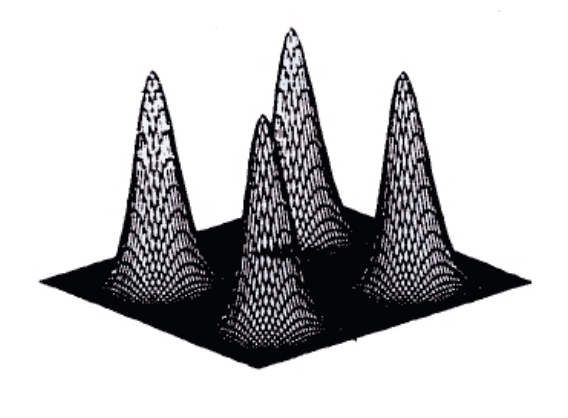
\includegraphics[width=8cm, keepaspectratio]{capitoli/immagini/imgs/puzzante.png}
    \caption{Nell'immagine possiamo osservare l'andamento pulsante della funzione campionante.}
\end{figure}

\section{Quantizzazione}
Per ottenere una completa discretizzazione di un'immagine è necessario
discretizzare, oltre al dominio, anche l'insieme immagine (insieme dei valori).
\begin{definition}
    Si definisce \textbf{quantizzazione} il procedimento di discretizzazione dei
    valori della funzione che rappresenta un'immagine, cioè il passaggio da
    valori continui a valori discreti.
\end{definition}
Per le immagini a toni di grigio si parla di \textbf{grey level quantization},
mentre per le immagini a colori si parla di \textbf{color depth}, in riferimento
al numero di bit utilizzati per ciascun canale di colore (8, 16, 24, 32 bit).
\begin{itemize}
    \item \textbf{Esempio 1:} Le immagini che siamo abituati a vedere tutti i giorni sui nostri cellulari
          sono immagini a colori a 8bit.
    \item \textbf{Esempio 2:} Nelle immagini mediche, di solito in formato
          \textbf{DICOM}, le immagini vengono rappresentate a 16bit ma gli
          ultimi 4 bit dell'immagine sono riservati ad informazioni personali
          che servono ad identificare il paziente che ha sostenuto l'esame.
\end{itemize}
\section{Immagine Digitale}
Tramite il campionamento e la quantizzazione è possibile definire un'immagine
digitale come segue:
\begin{definition}
    Una immagine digitale è una rappresentazione di matrici di elementi
    immagine, detti anche pixel (pixel = picture elements). Dove

    \begin{itemize}
        \item Il \textbf{pixel} costituisce la componente elementare della matrice,
              dove gli indici di riga e colonna indicano i valori delle due
              variabili spaziali, cioè la posizione di un punto nell'immagine.
        \item Ogni elemento della matrice contiene i valori che rappresentano
              l'intensità dei corrispondenti punti nell'immagine, anche detta
              \textbf{luminanza}.
    \end{itemize}
\end{definition}

\section{Campionamento per Immagini}
L'Immagine campionata è rappresentata tramite la seguente formula:

$$
    f_c(x,y) = f(x,y)s_c(x,y)=f(x,y)\sum_{j=-\infty}^{+\infty}
    \sum_{k=-\infty}^{+\infty} \delta (x-j \Delta x, y-k \Delta y)
$$

dove $s_c(x,y)$ è \textbf{la funzione campionante} e $\delta$ rappresenta
funzione \textbf{delta di Dirac} \TODO[]{Definire funzione di Dirac}.\\

Si può provare che c'è una relazione tra $\hat{f}_c$ e $\hat{f}$. Per questo è
importante assumere che lo spettro del segnale $f$ sia \textbf{a banda
    limitata}, cioè:

$$
    \hat{f}(\omega_x, \omega_y)=0 \text{ per } |\omega_x| > \bar{\omega}_x \text{ e } |\omega_y| > \bar{\omega}_y
$$
dove $\bar{\omega}_x$ e $\bar{\omega}_y$ definiscono la banda rettangolare dell'immagine.\\

Così lo spettro dell'immagine campionata consiste nello spettro dell'immagine
continua infinitamente ripetuta nel piano delle frequenze, in una griglia di
risoluzione ($\frac{2\pi}{\Delta x}, \frac{2 \pi}{\Delta y}$), dove:

$$
    (\frac{2\pi}{\Delta x}, \frac{2 \pi}{\Delta y}) = (w_{xc}, w_{yc})
$$

sono le \textbf{frequenze Sampling}.\\

Per ricostruire esattamente un segnale
campionato, la frequenza del campionamento non deve essere inferiore ad una
\textbf{frequenza minima (ovvero frequenza sampling)}, che corrisponde ad un
valore massimo per ciascuno degli intervalli $\Delta x$ , $\Delta y$.\\

Tale
valore minimo deve essere almeno pari al doppio della banda massima di $f$ ,
cioè:

\begin{equation}\label{eq:launo}
    \omega_{xc} \geq 2 \bar{\omega}_x \text{ e } \omega_{yc} \geq 2 \bar{\omega}_y
\end{equation}

o equivalentemente:

$$
    \frac{1}{\Delta x} \ge 2 \bar{\omega_x} \ \text{ e } \frac{1}{\Delta y} \ge 2 \bar{\omega_y}
$$
%% questa era LA UNO
Se nella (\ref{eq:launo}) vale l'uguaglianza, allora si dice che l'immagine è
\textbf{campionata alla sua frequenza di Nyquist.}\\

Se $\Delta x$ e $\Delta y$ sono più piccoli del richiesto criterio di
Nyquist, l'immagine risulta sovracampionata \textbf{(oversampling)}. Nel caso
contrario, l'immagine non può essere ricostruita esattamente: si parla di
sottocampionamento \textbf{(undersampling)} e si presenta un fenomeno di
distorsione detto \textbf{aliasing.}

\paragraph{Note:}
\begin{itemize}
    \item il valore minimo è un valore puramente teorico. Nella pratica, non
          potendo in generale determinare con precisione la banda massima del
          segnale, si utilizzano frequenze di campionamento più alte. Spesso
          si campiona con una frequenza pari a 4 volte quella misurata.
\end{itemize}

\begin{theorem}[Teorema del Campionamento per Immagini]
    Sia $f(x,y)$ un' immagine
    \begin{itemize}
        \item a banda limitata e ad energia finita, soddisfa quindi
              $$
                  \hat{f}(\omega_x,\omega_y) = 0 \text{ per } | \omega_x | >
                  \bar{\omega}_x \text{ e } | \omega_y | > \bar{\omega}_y;
              $$
        \item con $f$ uniformemente campionata in una
              griglia rettangolare con intervalli spaziali $\Delta x$, $\Delta y$,
        \item che abbia l'ordine di campionamento più grande dell'ordine di
              Nyquist, cioè
              $$
                  \omega_{xc} \geq 2 \bar{\omega}_x, \ \omega_{yc} \geq 2 \bar{\omega}_y
              $$
    \end{itemize}

    allora
    la $f$ può essere ricostruita dai suoi valori campione $f(j \Delta x, k
        \Delta y)$. Inoltre, l'immagine ricostruita è data dalla seguente formula di
    interpolazione:
\end{theorem}

$$
    f(x,y) = \sum_{j=-\infty}^{+\infty} \sum_{k=-\infty}^{+\infty} f(j \Delta
    x, k \Delta y) (\frac{\sin(xw_{xc}-j)\pi}{(xw_{xc}-j)\pi})
    (\frac{\sin(yw_{yc}-k)\pi}{(yw_{yc}-k)\pi})
$$

\section{L'aliasing}

Per ricostruire esattamente una immagine, è necessario limitare in banda
l'immagine che deve essere campionata, campionando all'ordine di campionamento
di Nyquist o più grande e interpolando appropriatamente i valori immagine.
\\\\Se c'è sovrapposizione di spettri, risultante dal sottocampionamento, vuol
dire che componenti spettrali spurie sono state introdotte nel processo di
ricostruzione. L'effetto che si ottiene è chiamato aliasing.

\begin{figure}[H]
    \centering
    \begin{tikzpicture}[x=0.75pt,y=0.75pt,yscale=-1,xscale=1]
        %uncomment if require: \path (0,300); %set diagram left start at 0, and has height of 300

        %Shape: Axis 2D [id:dp6614397845308091] 
        \draw  (204,230.75) -- (542.5,230.75)(306,82) -- (306,250.25) (535.5,225.75) -- (542.5,230.75) -- (535.5,235.75) (301,89) -- (306,82) -- (311,89)  ;
        %Straight Lines [id:da059819649685002974] 
        \draw    (424.6,225.95) -- (424.6,236.45) ;
        %Curve Lines [id:da1873728797992431] 
        \draw    (269.8,230.2) .. controls (290.2,149.8) and (320.6,150.6) .. (339.4,231) ;
        %Curve Lines [id:da5724817335486379] 
        \draw    (329.4,229.8) .. controls (349.8,149.4) and (380.2,150.2) .. (399,230.6) ;
        %Curve Lines [id:da36708092911214907] 
        \draw    (388.2,230.6) .. controls (408.6,150.2) and (439,151) .. (457.8,231.4) ;
        %Curve Lines [id:da8399376612652416] 
        \draw    (211,229.8) .. controls (231.4,149.4) and (261.8,150.2) .. (280.6,230.6) ;
        %Straight Lines [id:da03322400871511211] 
        \draw  [dash pattern={on 0.84pt off 2.51pt}]  (365,170.2) -- (364.8,230.35) ;
        %Straight Lines [id:da4711905178599287] 
        \draw  [dash pattern={on 0.84pt off 2.51pt}]  (424.6,171) -- (424.4,231.15) ;
        %Straight Lines [id:da6104769152801106] 
        \draw  [dash pattern={on 0.84pt off 2.51pt}]  (246.2,170.6) -- (246,230.75) ;
        %Straight Lines [id:da17157099933830633] 
        \draw    (364.8,225.15) -- (364.8,235.65) ;
        %Straight Lines [id:da303351675318031] 
        \draw    (246.2,224.75) -- (246.2,235.25) ;
        %Shape: Free Drawing [id:dp8099197566718934] 
        \draw  [color={rgb, 255:red, 255; green, 0; blue, 0 }  ,draw opacity=1 ][line width=0.75] [line join = round][line cap = round] (275.67,216.17) .. controls (275.67,216.17) and (275.67,216.17) .. (275.67,216.17) ;
        %Shape: Free Drawing [id:dp2110659887332691] 
        \draw  [color={rgb, 255:red, 255; green, 0; blue, 0 }  ,draw opacity=1 ][line width=0.75] [line join = round][line cap = round] (275,218.17) .. controls (275,218.28) and (275,218.39) .. (275,218.5) ;
        %Shape: Free Drawing [id:dp06278082285778552] 
        \draw  [color={rgb, 255:red, 255; green, 0; blue, 0 }  ,draw opacity=1 ][line width=0.75] [line join = round][line cap = round] (275.33,218.83) .. controls (275.44,218.94) and (275.56,219.06) .. (275.67,219.17) ;
        %Shape: Free Drawing [id:dp19051968150897824] 
        \draw  [color={rgb, 255:red, 255; green, 0; blue, 0 }  ,draw opacity=1 ][line width=0.75] [line join = round][line cap = round] (275.33,219.17) .. controls (275.56,219.83) and (275.78,220.5) .. (276,221.17) ;
        %Shape: Free Drawing [id:dp6214978798746364] 
        \draw  [color={rgb, 255:red, 255; green, 0; blue, 0 }  ,draw opacity=1 ][line width=0.75] [line join = round][line cap = round] (275.67,219.83) .. controls (276.11,220.39) and (276.56,220.94) .. (277,221.5) ;
        %Shape: Free Drawing [id:dp9117399273678792] 
        \draw  [color={rgb, 255:red, 255; green, 0; blue, 0 }  ,draw opacity=1 ][line width=0.75] [line join = round][line cap = round] (277.33,221.5) .. controls (278.33,222.17) and (278.86,223.4) .. (279.33,224.5) ;
        %Shape: Free Drawing [id:dp9439140035486251] 
        \draw  [color={rgb, 255:red, 255; green, 0; blue, 0 }  ,draw opacity=1 ][line width=0.75] [line join = round][line cap = round] (277.33,223.17) .. controls (277.22,223.17) and (277.11,223.17) .. (277,223.17) ;
        %Shape: Free Drawing [id:dp30388898253809615] 
        \draw  [color={rgb, 255:red, 255; green, 0; blue, 0 }  ,draw opacity=1 ][line width=0.75] [line join = round][line cap = round] (275,221.83) .. controls (274.89,222.72) and (274.78,223.61) .. (274.67,224.5) ;
        %Shape: Free Drawing [id:dp1381324474200707] 
        \draw  [color={rgb, 255:red, 255; green, 0; blue, 0 }  ,draw opacity=1 ][line width=0.75] [line join = round][line cap = round] (275.67,223.17) .. controls (276.22,223.72) and (276.78,224.28) .. (277.33,224.83) ;
        %Shape: Free Drawing [id:dp8005021491573696] 
        \draw  [color={rgb, 255:red, 255; green, 0; blue, 0 }  ,draw opacity=1 ][line width=0.75] [line join = round][line cap = round] (277.67,225.5) .. controls (277.67,226.61) and (277.67,227.72) .. (277.67,228.83) ;
        %Shape: Free Drawing [id:dp2674763078018507] 
        \draw  [color={rgb, 255:red, 255; green, 0; blue, 0 }  ,draw opacity=1 ][line width=0.75] [line join = round][line cap = round] (276.67,228.17) .. controls (276.33,227.83) and (276,227.5) .. (275.67,227.17) ;
        %Shape: Free Drawing [id:dp7006529540548063] 
        \draw  [color={rgb, 255:red, 255; green, 0; blue, 0 }  ,draw opacity=1 ][line width=0.75] [line join = round][line cap = round] (274.33,226.17) .. controls (274.33,225.94) and (274.33,225.72) .. (274.33,225.5) ;
        %Shape: Free Drawing [id:dp12114685025543515] 
        \draw  [color={rgb, 255:red, 255; green, 0; blue, 0 }  ,draw opacity=1 ][line width=0.75] [line join = round][line cap = round] (274.33,222.83) .. controls (274.33,222.94) and (274.33,223.06) .. (274.33,223.17) ;
        %Shape: Free Drawing [id:dp11181613935726564] 
        \draw  [color={rgb, 255:red, 255; green, 0; blue, 0 }  ,draw opacity=1 ][line width=0.75] [line join = round][line cap = round] (272.33,227.5) .. controls (272.44,227.61) and (272.56,227.72) .. (272.67,227.83) ;
        %Shape: Free Drawing [id:dp21874941104891454] 
        \draw  [color={rgb, 255:red, 255; green, 0; blue, 0 }  ,draw opacity=1 ][line width=0.75] [line join = round][line cap = round] (276.33,226.5) .. controls (276.33,226.5) and (276.33,226.5) .. (276.33,226.5) ;
        %Shape: Free Drawing [id:dp1551213334904571] 
        \draw  [color={rgb, 255:red, 255; green, 0; blue, 0 }  ,draw opacity=1 ][line width=0.75] [line join = round][line cap = round] (336,225.5) .. controls (336,225.5) and (336,225.5) .. (336,225.5) ;
        %Shape: Free Drawing [id:dp5552556558692121] 
        \draw  [color={rgb, 255:red, 255; green, 0; blue, 0 }  ,draw opacity=1 ][line width=0.75] [line join = round][line cap = round] (335.67,223.83) .. controls (335.44,223.61) and (335.22,223.39) .. (335,223.17) ;
        %Shape: Free Drawing [id:dp2680712522684394] 
        \draw  [color={rgb, 255:red, 255; green, 0; blue, 0 }  ,draw opacity=1 ][line width=0.75] [line join = round][line cap = round] (335,222.5) .. controls (334.78,222.06) and (334.56,221.61) .. (334.33,221.17) ;
        %Shape: Free Drawing [id:dp7973466921888765] 
        \draw  [color={rgb, 255:red, 255; green, 0; blue, 0 }  ,draw opacity=1 ][line width=0.75] [line join = round][line cap = round] (334,223.17) .. controls (333.67,223.72) and (333.33,224.28) .. (333,224.83) ;
        %Shape: Free Drawing [id:dp4217427243501193] 
        \draw  [color={rgb, 255:red, 255; green, 0; blue, 0 }  ,draw opacity=1 ][line width=0.75] [line join = round][line cap = round] (331.67,227.83) .. controls (331.67,227.83) and (331.67,227.83) .. (331.67,227.83) ;
        %Shape: Free Drawing [id:dp7263061231203432] 
        \draw  [color={rgb, 255:red, 255; green, 0; blue, 0 }  ,draw opacity=1 ][line width=0.75] [line join = round][line cap = round] (334,227.83) .. controls (334,227.83) and (334,227.83) .. (334,227.83) ;
        %Shape: Free Drawing [id:dp5942130285250151] 
        \draw  [color={rgb, 255:red, 255; green, 0; blue, 0 }  ,draw opacity=1 ][line width=0.75] [line join = round][line cap = round] (334.33,227.83) .. controls (334.33,227.83) and (334.33,227.83) .. (334.33,227.83) ;
        %Shape: Free Drawing [id:dp15743052029399962] 
        \draw  [color={rgb, 255:red, 255; green, 0; blue, 0 }  ,draw opacity=1 ][line width=0.75] [line join = round][line cap = round] (335.33,227.83) .. controls (335.78,228.06) and (336.22,228.28) .. (336.67,228.5) ;
        %Shape: Free Drawing [id:dp22495918083215116] 
        \draw  [color={rgb, 255:red, 255; green, 0; blue, 0 }  ,draw opacity=1 ][line width=0.75] [line join = round][line cap = round] (334.67,226.5) .. controls (334.67,226.5) and (334.67,226.5) .. (334.67,226.5) ;
        %Shape: Free Drawing [id:dp2784909236606581] 
        \draw  [color={rgb, 255:red, 255; green, 0; blue, 0 }  ,draw opacity=1 ][line width=0.75] [line join = round][line cap = round] (336.33,220.83) .. controls (336.33,220.94) and (336.33,221.06) .. (336.33,221.17) ;
        %Shape: Free Drawing [id:dp8706240640891032] 
        \draw  [color={rgb, 255:red, 255; green, 0; blue, 0 }  ,draw opacity=1 ][line width=0.75] [line join = round][line cap = round] (335.33,220.5) .. controls (335.22,220.5) and (335.11,220.5) .. (335,220.5) ;
        %Shape: Free Drawing [id:dp9329750308424989] 
        \draw  [color={rgb, 255:red, 255; green, 0; blue, 0 }  ,draw opacity=1 ][line width=0.75] [line join = round][line cap = round] (392.67,227.83) .. controls (393,228.06) and (393.33,228.28) .. (393.67,228.5) ;
        %Shape: Free Drawing [id:dp3882317480429962] 
        \draw  [color={rgb, 255:red, 255; green, 0; blue, 0 }  ,draw opacity=1 ][line width=0.75] [line join = round][line cap = round] (395,228.17) .. controls (395.63,228.8) and (395.3,228.46) .. (394.67,227.83) ;
        %Shape: Free Drawing [id:dp4131517984324593] 
        \draw  [color={rgb, 255:red, 255; green, 0; blue, 0 }  ,draw opacity=1 ][line width=0.75] [line join = round][line cap = round] (394.33,224.5) .. controls (395,224.83) and (395.67,225.17) .. (396.33,225.5) ;
        %Shape: Free Drawing [id:dp37363169850637656] 
        \draw  [color={rgb, 255:red, 255; green, 0; blue, 0 }  ,draw opacity=1 ][line width=0.75] [line join = round][line cap = round] (394,227.83) .. controls (393.78,227.5) and (393.56,227.17) .. (393.33,226.83) ;
        %Shape: Free Drawing [id:dp11367818680791109] 
        \draw  [color={rgb, 255:red, 255; green, 0; blue, 0 }  ,draw opacity=1 ][line width=0.75] [line join = round][line cap = round] (393,219.83) .. controls (392.89,219.5) and (392.78,219.17) .. (392.67,218.83) ;
        %Shape: Free Drawing [id:dp0009232964570280444] 
        \draw  [color={rgb, 255:red, 255; green, 0; blue, 0 }  ,draw opacity=1 ][line width=0.75] [line join = round][line cap = round] (394.33,220.5) .. controls (394.67,221.17) and (395,221.83) .. (395.33,222.5) ;
        %Shape: Free Drawing [id:dp980765288470274] 
        \draw  [color={rgb, 255:red, 255; green, 0; blue, 0 }  ,draw opacity=1 ][line width=0.75] [line join = round][line cap = round] (392.33,219.83) .. controls (392.33,221.28) and (392.33,222.72) .. (392.33,224.17) ;
        %Shape: Free Drawing [id:dp18690833347628333] 
        \draw  [color={rgb, 255:red, 255; green, 0; blue, 0 }  ,draw opacity=1 ][line width=0.75] [line join = round][line cap = round] (394,224.17) .. controls (394.11,224.17) and (394.22,224.17) .. (394.33,224.17) ;
        %Shape: Free Drawing [id:dp5757936876425502] 
        \draw  [color={rgb, 255:red, 255; green, 0; blue, 0 }  ,draw opacity=1 ][line width=0.75] [line join = round][line cap = round] (392.67,225.17) .. controls (392.67,225.17) and (392.67,225.17) .. (392.67,225.17) ;
        %Shape: Free Drawing [id:dp3612108432226979] 
        \draw  [color={rgb, 255:red, 255; green, 0; blue, 0 }  ,draw opacity=1 ][line width=0.75] [line join = round][line cap = round] (392.67,226.5) .. controls (392.89,226.61) and (393.11,226.72) .. (393.33,226.83) ;
        %Shape: Free Drawing [id:dp7648800367951516] 
        \draw  [color={rgb, 255:red, 255; green, 0; blue, 0 }  ,draw opacity=1 ][line width=0.75] [line join = round][line cap = round] (394.67,218.83) .. controls (394.67,218.83) and (394.67,218.83) .. (394.67,218.83) ;
        %Shape: Free Drawing [id:dp1400767539639749] 
        \draw  [color={rgb, 255:red, 255; green, 0; blue, 0 }  ,draw opacity=1 ][line width=0.75] [line join = round][line cap = round] (397.67,226.17) .. controls (397.67,226.5) and (397.67,226.83) .. (397.67,227.17) ;
        %Straight Lines [id:da9749345597918087] 
        \draw [color={rgb, 255:red, 0; green, 0; blue, 0 }  ,draw opacity=1 ]   (394.33,138.5) -- (394.33,197.83) ;
        \draw [shift={(394.33,199.83)}, rotate = 270] [color={rgb, 255:red, 0; green, 0; blue, 0 }  ,draw opacity=1 ][line width=0.75]    (10.93,-3.29) .. controls (6.95,-1.4) and (3.31,-0.3) .. (0,0) .. controls (3.31,0.3) and (6.95,1.4) .. (10.93,3.29)   ;
        %Straight Lines [id:da9406931472834237] 
        \draw    (394.33,138.5) -- (450.67,138.83) ;
        %Straight Lines [id:da7746905723182127] 
        \draw  [dash pattern={on 0.84pt off 2.51pt}]  (339.07,151) -- (339.4,231) ;
        %Straight Lines [id:da7675893385629211] 
        \draw    (305.67,150.17) -- (337.07,150.95) ;
        \draw [shift={(339.07,151)}, rotate = 181.43] [color={rgb, 255:red, 0; green, 0; blue, 0 }  ][line width=0.75]    (10.93,-3.29) .. controls (6.95,-1.4) and (3.31,-0.3) .. (0,0) .. controls (3.31,0.3) and (6.95,1.4) .. (10.93,3.29)   ;

        % Text Node
        \draw (308.8,231.8) node [anchor=north west][inner sep=0.75pt]   [align=left] {0};
        % Text Node
        \draw (356,239.4) node [anchor=north west][inner sep=0.75pt]    {$f_{S}$};
        % Text Node
        \draw (411.2,240.6) node [anchor=north west][inner sep=0.75pt]    {$2f_{S}$};
        % Text Node
        \draw (230.4,240.2) node [anchor=north west][inner sep=0.75pt]    {$-f_{S}$};
        % Text Node
        \draw (398.67,119.67) node [anchor=north west][inner sep=0.75pt]   [align=left] {Aliasing};
        % Text Node
        \draw (309.67,128.73) node [anchor=north west][inner sep=0.75pt]    {$f_{m}$};
    \end{tikzpicture}
    \caption{Visualizzazione della sovrapposizione degli spettri che genera aliasing}
\end{figure}

Quindi l'aliasing è la presenza di componenti spettrali (frequenze) indesiderate
nella ricostruzione dell'immagine, componenti che non erano presenti quando
l'immagine originale era stata campionata.

\begin{figure}[H]
    \centering
    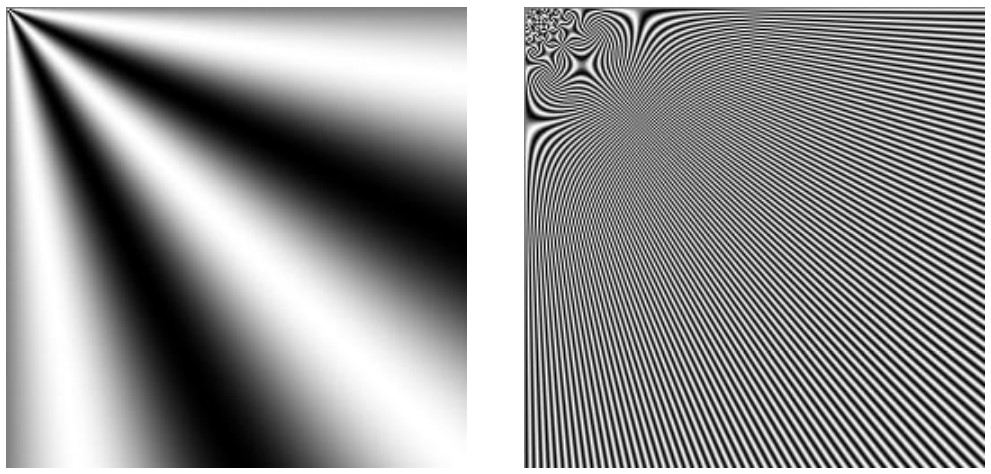
\includegraphics[width=10cm, keepaspectratio]{capitoli/immagini/imgs/aliasing_componenti_spettrali.jpg}
    \caption{Esempio di frequenze indesiderate prodotte dall'aliasing.}
\end{figure}

L'aliasing deriva dal sottocampionamento e causa perdita di risoluzione
dell'immagine campionata (effetto scacchiera).

\begin{figure}[H]
    \centering
    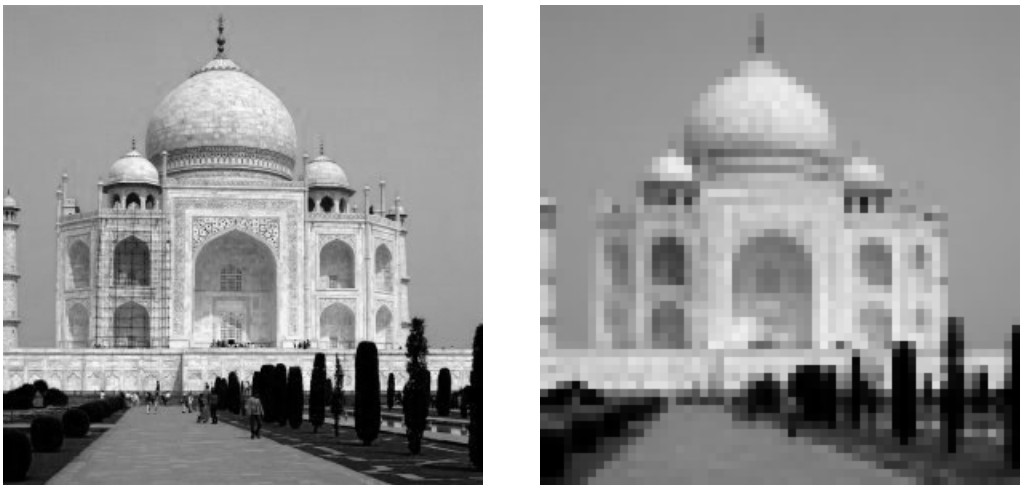
\includegraphics[width=10cm, keepaspectratio]{capitoli/immagini/imgs/aliasing_tajmahal.jpg}
    \caption{Esempio di effetto a scacchiera generato dall'aliasing}.
\end{figure}

\begin{itemize}
    \item Per prevenire aliasing di queste componenti, è possibile filtrarle via
          (eliminarle) prima di campionare il segnale. Eliminare certe frequenze
          e lasciare passare le basse frequenze, è una operazione nota come
          \textbf{filtraggio passa-basso}.
    \item Ogni attenuazione relativa a questo processo di filtraggio rappresenta
          una perdita di risoluzione dell'immagine campionata.
    \item Come risultato, mentre da un lato c'è una perdita della risoluzione
          dell'immagine campionata, dall'altro c'è una attenuazione
          dell'aliasing error.
    \item \textbf{Effetto Moirè:} ovvero la distorsione visiva che si manifesta
          quando due griglie si sovrappongono
          \begin{figure}[H]
              \centering
              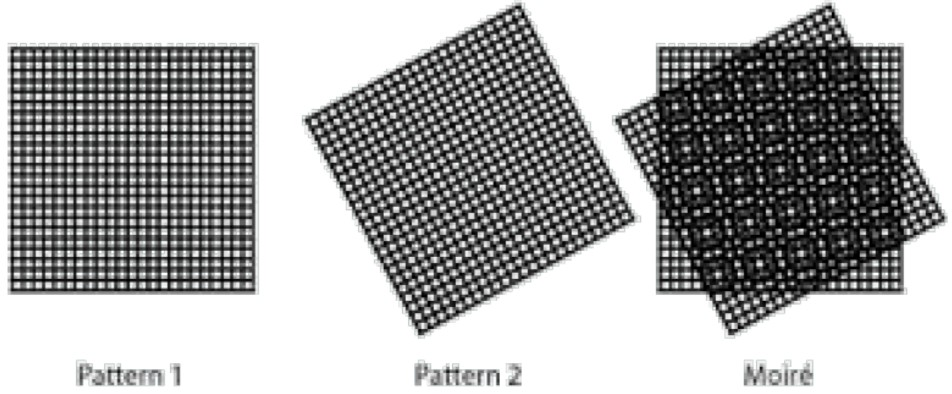
\includegraphics[width=8cm, keepaspectratio]{capitoli/immagini/imgs/effetto_moire.jpg}
          \end{figure}
\end{itemize}

\section{La risoluzione}
Il campionamento e la quantizzazione determinano la \textbf{risoluzione}
dell'immagine. \\

La \textbf{risoluzione} di un segnale è un indice del grado
di qualità dell'immagine: misura il grado di oggetti distinguibili
nell'immagine. Esistono differenti definizione di risoluzione:

\begin{definition}
    La \textbf{Risoluzione Spaziale} indica la densità dei campioni, ovvero è data dal numero di campioni
    per unità di area.
\end{definition}

Spesso è espressa come numero di pixel
nell'unità di lunghezza e viene misurata in pixel per pollice (ppi).
\\Un'immagine ad alta risoluzione contiene più pixel di una delle
stesse dimensioni con una risoluzione inferiore, quindi è in grado di
riprodurre un maggior numero di dettagli. Un'elevata risoluzione
comporta tuttavia un aumento considerevole delle dimensioni (quantità
di dati) dell'immagine.

\paragraph{Esempio:}

Un'immagine di $1cm \times 1cm$ con una risoluzione di 72 ppi
contiene 5184 pixel ($72 \times 72$). La stessa immagine di $1 cm \times
    1 cm$ a 300 ppi conterrebbe 90.000 pixel.

\begin{definition}
    La \textbf{Risoluzione spettrale} indica la banda passante del sensore.

\end{definition}


\begin{definition}
    \textbf{Risoluzione radiometrica} indica il numero di livelli di quantizzazione.

\end{definition}


\begin{definition}
    \textbf{Risoluzione temporale} indica la frequenza di acquisizione dei frames di un'immagine in
    movimento.
\end{definition}

\section{Alterazioni della risoluzione}

Alterando i vari tipi di risoluzione, l'immagine presenterà di volta in volta un
diverso tipo di distorsione.

\begin{trivlist}
    \item \textbf{Risoluzione spaziale:} diminuendo la risoluzione spaziale
    (nell'esempio di un quarto) si ottiene il tipico effetto ”quadrettato”,
    detto anche a scacchiera, dovuto all'aliasing.
    \begin{figure}[H]
        \centering
        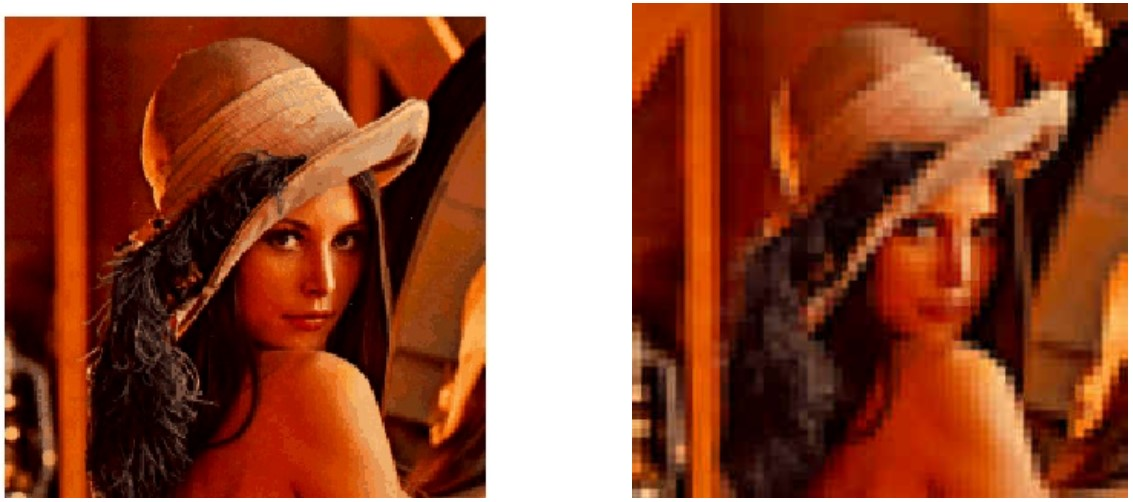
\includegraphics[width=10cm, keepaspectratio]{capitoli/immagini/imgs/esempio_risoluzione_spaziale.jpg}
    \end{figure}

    \item \textbf{Risoluzione spettrale:} Diminuendo la banda passante del
    sensore di acquisizione dell'immagine si ottiene un'immagine più ”sfocata”,
    in quanto i dettagli ad alta frequenza spaziale vanno persi.
    \begin{figure}[H]
        \centering
        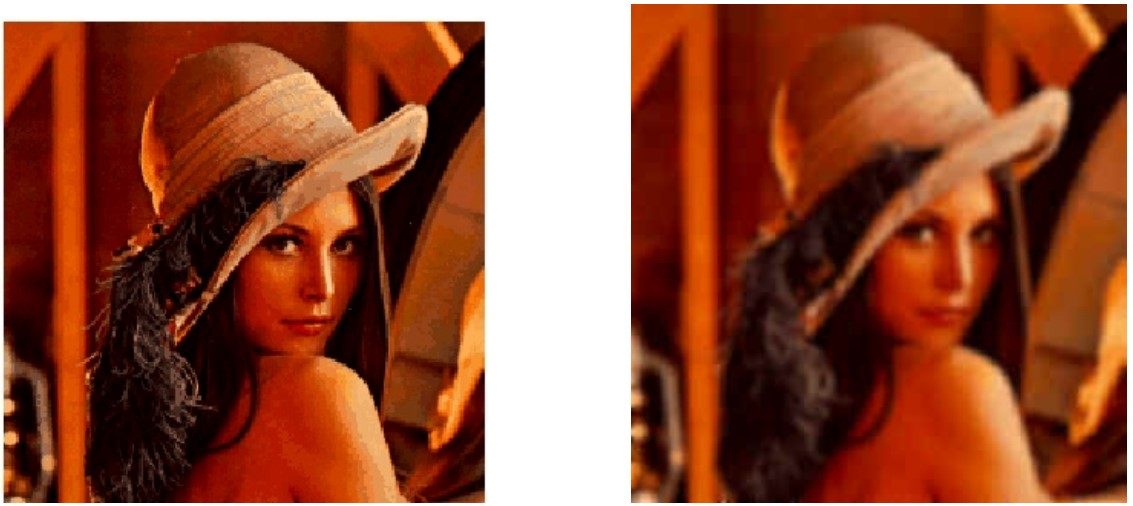
\includegraphics[width=10cm, keepaspectratio]{capitoli/immagini/imgs/esempio_risoluzione_spettrale.jpg}
    \end{figure}

    \item \textbf{Risoluzione radiometrica:} Diminuendo la profondità di colore,
    si distinguono in maniera più marcata i passaggi da un colore ad un altro;
    essi risultano pertanto sempre più accentuati e meno graduali, fino a
    produrre dei "falsi contorni" (variazioni di ombreggiatura).
    \begin{figure}[H]
        \centering
        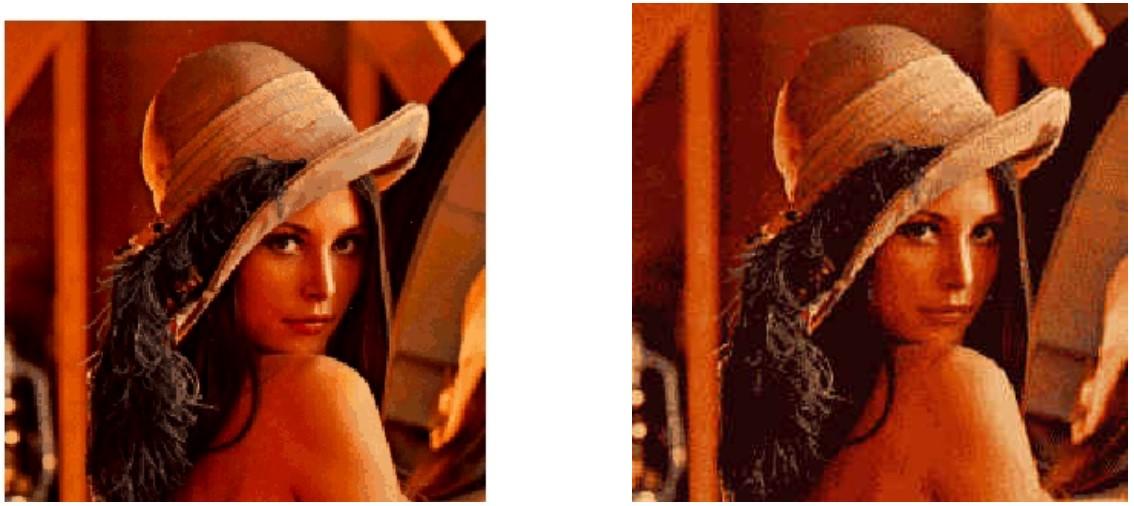
\includegraphics[width=10cm, keepaspectratio]{capitoli/immagini/imgs/esempio_risoluzione_radiometrica.jpg}
    \end{figure}
\end{trivlist}

\section{Immagini in bianco e nero e immagini a colori}

\subsection{Immagini in bianco e nero}

Un'\textbf{immagine in bianco e nero (b/w)} è caratterizzata da una
rappresentazione binaria, ovvero la funzione che la rappresenta in
ogni punto ($x$ , $y$) può assumere solo due valori: 0 e 1. In genere,
ad 1 si associa il bianco, mentre a 0 il nero.

\begin{figure}[H]
    \centering
    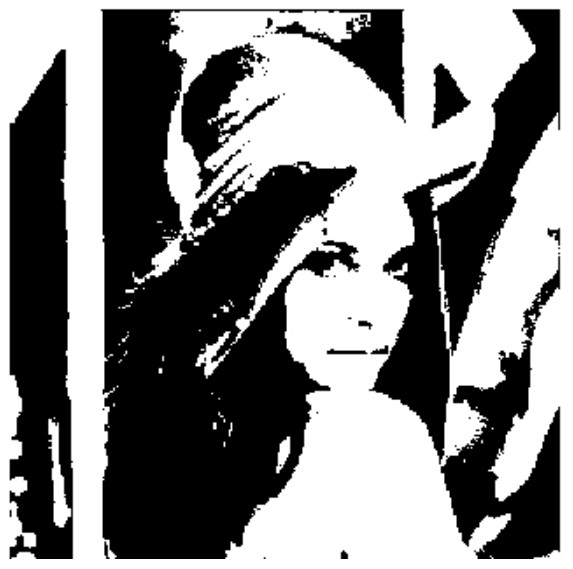
\includegraphics[width=4cm, keepaspectratio]{capitoli/immagini/imgs/immagine_binaria_bianco_nero.jpg}
    \caption{Esempio di un'immagine in bianco e nero (binaria).}
\end{figure}

\subsection{Immagini a toni di grigio}

Un'immagine a toni di grigio è rappresentata da una matrice le cui
entrate sono i valori che la funzione $f$ assume in ogni punto.

\begin{figure}[H]
    \centering
    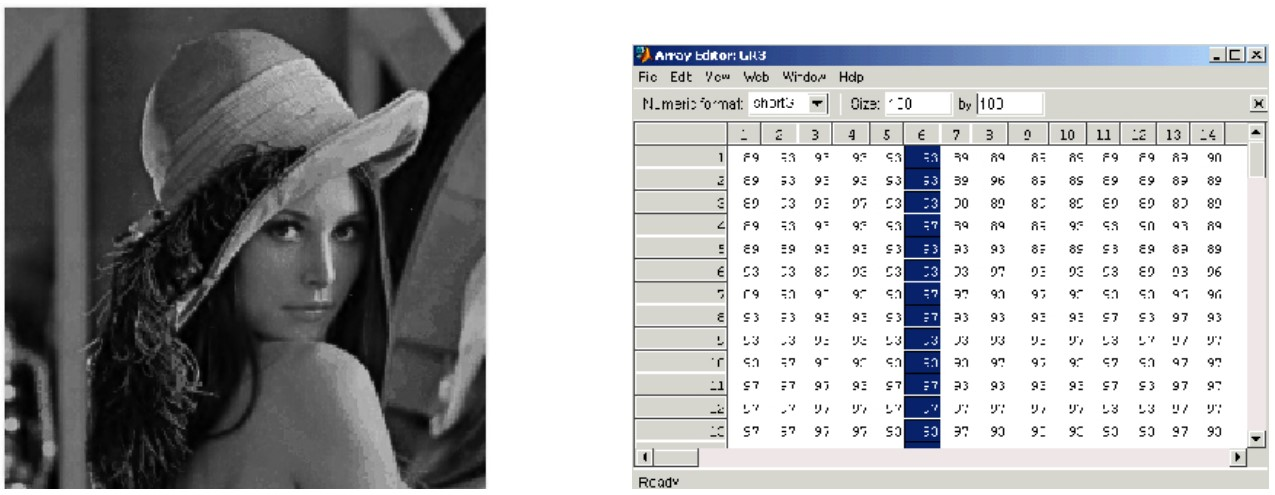
\includegraphics[width=12cm, keepaspectratio]{capitoli/immagini/imgs/rappresentazione_immagine_toni_grigio.jpg}
\end{figure}

In genere, si assume che i \textbf{livelli di grigio} siano discreti ed
equispaziati in un intervallo di valori normalmente \textbf{tra 0 e 255}:
esistono allora un massimo di 256 livelli di grigio.
\\
La funzione $f (x , y)$ può essere rappresentata come una superficie
nello spazio.

\begin{figure}[H]
    \centering
    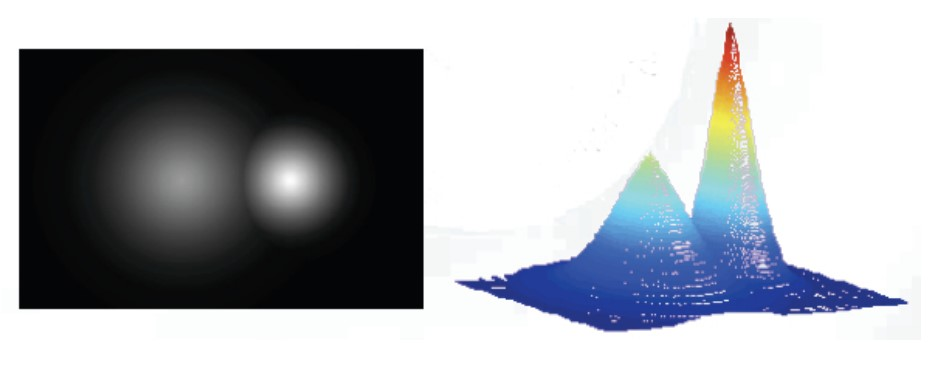
\includegraphics[width=10cm, keepaspectratio]{capitoli/immagini/imgs/funzione_toni_grigio.jpg}
\end{figure}

\subsection{Immagini a colori}

Per rappresentare un'\textbf{immagine a colori} è necessario ricorrere ad
una funzione vettoriale. Un colore infatti può essere sempre
decomposto come \textbf{somma dei tre colori fondamentali (rosso, verde,
    blu)}, ciascuno con un'opportuna intensità.
Un'immagine a colori, dunque, può essere rappresentata da una
funzione $f: \mathbb{R}^2 \rightarrow \mathbb{R}^3$ del tipo

$$
    f(x, y) = [R(x, y), G(x, y), B(x, y)]
$$

Questo tipo di rappresentazione viene detta \textbf{RGB (Red,Green,Blue)}.
\subsubsection{Lo spazio RGB}

Lo spazio RGB è uno spazio cartesiano, con tre assi ortogonali.
Il colore di ciascun pixel viene rappresentato da un vettore
$[R(x , y), G(x , y), B(x , y)]$ nello spazio RGB; ogni componente
indica la quantità di rosso, verde e blu, rispettivamente, necessari
ad ottenere quel colore.
In base alla rappresentazione RGB, un'immagine a colori viene
rappresentata da una terna di matrici, ognuna delle quali contiene i
valori relativi ad un canale di colore.\\
Ogni canale, preso a sè, non è altro che un'immagine a toni di
grigio.

\begin{figure}[H]
    \centering
    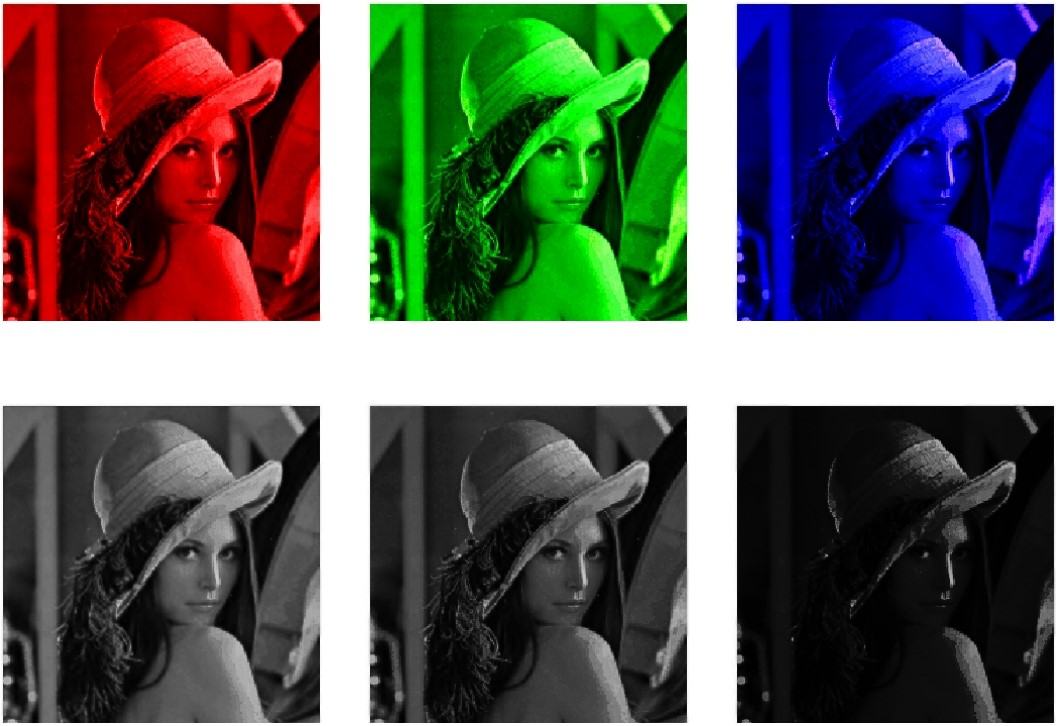
\includegraphics[width=12cm, keepaspectratio]{capitoli/immagini/imgs/canali_RGB_e_grigio.jpg}
\end{figure}

\subsubsection{Lo spazio HSV}

Oltre alla RGB esistono anche altri tipi di rappresentazioni (che
possono essere in genere derivate da essa).
Una di queste è la rappresentazione \textbf{HSV}. Lo spazio HSV ha un
sistema di coordinate cilindrico con due assi ortogonali ed un
angolo di rotazione intorno ad uno dei due assi.
L'altezza del cono rappresenta la \textbf{luminosità (Value)}, con valori da
0 (nero) a 1 (bianco). La \textbf{saturazione (Saturation)} indica l'intensità
e la purezza del colore, con valori da 0 (sull'asse del cono) a 1
(sulla superficie del cono). La terza coordinata rappresenta la
\textbf{tonalità di colore (Hue)} e viene misurata da un angolo intorno
all'asse verticale (rosso a 0 gradi, verde a 120 e blu a 240).

\begin{figure}[H]
    \centering
    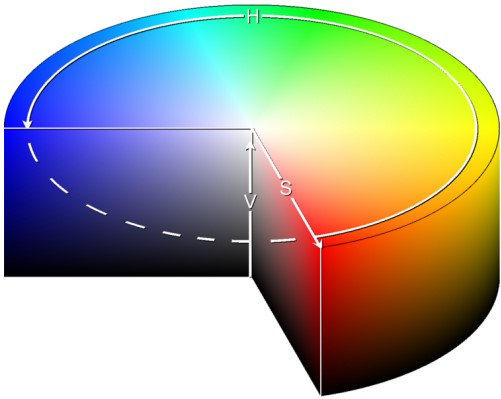
\includegraphics[width=5cm, keepaspectratio]{capitoli/immagini/imgs/cilindro_hsv.jpg}
\end{figure}


\section{Relazioni di base fra pixel}

\subsection{Intorni}

Un pixel $p$ di coordinate $(x,y)$ ha quattro \textbf{neighbors} (vicini) orizzontali e verticali:

\begin{center}
    $(x+1, y), (x-1, y), (x, y-1), (x, y+1)$
\end{center}

Questi punti formano il \textbf{4-intorno (4-neighboor)} di $(x,y)$ che indicheremo con $N_4(p)$
\\I quattro \textbf{neighbors (vicini) diagonali} di $p$ $(N_D(p))$ hanno invece coordinate

\begin{center}
    $(x+1, y+1), (x+1,y-1), (x-1, y+1), (x-1, y-1)$
\end{center}

I vicini diagonali, insieme a quelli orizzontali e verticali, formano l'\textbf{8-intorno (8-neighbor)} di $(x,y)$  che indicheremo con $N_8(p)$

\subsection{Connettività e adiacenza}

Due pixel sono connessi se sono vicini e presentano livelli di intensità con una certa relazione (ad esempio hanno lo stesso livello di grigio).
Fissato un insieme V di valori di intensità, due pixel $p$ e $q$ si dicono

\begin{itemize}
    \item \textbf{4-adiacenti} se i valori di entrambi appartengono a $V$ e $q \in N_4(p)$
    \item \textbf{8-adiacenti} se i valori di entrambi appartengono a $V$ e $q \in N_8(p)$
    \item \textbf{m-adiacenti} (adiacenza mista) se i valori di entrambi appartengono a $V$ e $q \in N_4(p)$ oppure $q \in N_D(p)$ e l'insieme $N_4(p) \cap N_4(q)$ non contiene pixel a valori in V.
\end{itemize}

\subsection{Cammini}

Un \textbf{cammino (path) digitale} dal pixel $p = (x,y)$ al pixel $q = (x',
    y')$ è una sequenza di pixel

\begin{center}
    $(x0, y0), (x1, y1), ... ,(x_n, y_n)$
\end{center}

dove $(x_0, y_0) = (x,y)$, $(x_n, y_n) = (x', y')$ e i pixel $(x_i, y_i)$,
$(x_{i+1}, y_{i+1})$ sono adiacenti per ogni $i=0, ... , n-1$, dove $n$ è la
\textbf{lunghezza del cammino}. $Se (x_0, y_0) = (x_n, y_n)$ si parla di
\textbf{cammino chiuso}. Si puo' definire in particolare un $4-$, $8-$, o
$m-$ cammino restringendo l'adiacenza alla corrispondente tipologia.

\subsection{Cammini e regioni}

Fissato un sottoinsieme $S$ di pixel di un'immagine digitale, due pixel p e q si
dicono \textbf{connessi} se esiste un cammino tra $p$ e $q$ che consiste di
pixel tutti contenuti in $S$. \\Se tutti i pixel di $S$ sono connessi, $S$ si
dice un insieme connesso: in tal caso diciamo che $S$ è una regione
dell'immagine. Il \textbf{bordo (boundary, border, contour)} di una regione $R$
è l'insieme dei pixel di $R$ che hanno uno o più vicini che non appartengono ad
R. Nel caso in cui $R$ sia l'intera immagine, il bordo si definisce come la
prima e l'ultima riga e la prima e l'ultima colonna. \\Se l'immagine contiene
$k$ regioni distinte $R_1,..., R_k$, nessuna delle quali tocca i bordi
dell'immagine, allora l'unione $R = \cup_{i=1}^n R_i$ si dice \textbf{primo
    piano (foreground)}, mentre il complementare $R^c$ viene detto
\textbf{sfondo(background)}.

\subsection{Distanza tra pixel}

Una distanza (o metrica) tra pixel è una funzione $D(p, q)$ tale che per ogni
$p, q, z$

\begin{itemize}
    \item $D(p, q) \ge 0$
    \item $D(p, q) = 0$ se e solo se $p = q$
    \item $D(p, q) = D(q, p)$
    \item $D(p, z) \le D(p, q) + D(q, z)$
\end{itemize}

\textbf{Esempi}

\begin{itemize}
    \item Distanza euclidea: $D_e(p, q) = \{(x_1 - x_2)^2 + (y_1 - y_2)^2\}^{\frac{1}{2}}$, se $p = (x_1, y_1), q=(x_2, y_2)$
    \item Distanza $D_4$, o city-block: $D_4(p, q) = |x_1 - x_2| + |y_1 - y_2|$.
    \item Distanza $D_8$, o a scacchiera: $D_s(p,q) = max\{|x_1 - x_2|, |y_1 - y_2|\}$
\end{itemize}

\chapter{Elaborazione con Filtri}

L'elaborazione delle immagini è una disciplina che prevede l'utilizzo
di algoritmi i quali operano sui pixel che compongono l'immagine
e, applicando trasformazioni numeriche, restituiscono un'immagine
modificata.\\
Le tecniche di elaborazione delle immagini hanno vari scopi, fra cui:

\begin{itemize}
    \item il miglioramento della qualità dell'immagine (\textbf{image enhancement})
    \item il ripristino della qualità dell'immagine (\textbf{image restoration})
    \item l'estrazione di informazioni sul contenuto dell'immagine (\textbf{image analysis})
\end{itemize}

\paragraph{Note:}

\begin{itemize}
    \item L'\textbf{image analysis} è una parte fondamentale della computer vision e
          precede l'\textbf{image recognition}.\\
          Essa può richiedere elaborazioni differenti a seconda del tipo di
          informazione che si vuole estrarre: tra queste, le elaborazioni nel
          dominio spaziale, nel dominio delle frequenze, con riduzione dei
          dati tra ingresso e uscita (compressione), etc.
\end{itemize}

\paragraph{Esempio:}

Un'elaborazione nel dominio spaziale, può essere
espressa come

$$
    g(x , y) = T(f (x , y))
$$

\begin{itemize}
    \item $f$ è l'immagine di ingresso
    \item $g$ è l'immagine di uscita
    \item $T$ è un operatore su f, definito in un intorno di $(x , y)$.
\end{itemize}

La natura dell'intorno definisce il tipo di elaborazione e si distingue,
in particolare, fra: \textbf{elaborazioni puntuali}, \textbf{locali} e \textbf{globali}.

\begin{definition}
    Le elaborazioni \textbf{puntuali} trasformano il valore di un pixel sulla
    base del valore del pixel stesso.
\end{definition}

\begin{definition}
    Le elaborazioni \textbf{locali} lavorano sulla base dei valori assunti dai pixel in
    un intorno di quello preso in esame.
\end{definition}

\begin{definition}
    Le elaborazioni \textbf{globali} trasformano il valore di un pixel sulla
    base dei valori assunti da tutti i pixel dell'immagine.
\end{definition}

\section{Elaborazioni Locali}

\subsection{Zoom}

Si crea una nuova griglia, ovvero delle nuove "locazioni" per i pixel,
sovrapponendola a quella originale; si assegnano poi i livelli di grigio a
queste nuove locazioni.

\begin{itemize}
    \item \textbf{Nearest Neighbor:} assegna ad ogni nuova locazione l'intensità
          del pixel più vicino dell'immagine originale

    \item \textbf{Interpolazione bilineare:} prevede l'utilizzo dei quattro
          pixel più vicini per stimare l'intensità da assegnare ad ogni nuova
          locazione

          \begin{figure}[H]
              \centering
              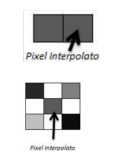
\includegraphics[width=3cm, keepaspectratio]{capitoli/immagini/imgs/esempio-interpolazione.png}
          \end{figure}

          $$
              f(x,y)=ax+by+cxy+d
          $$

          dove i coefficienti $a, b, c, d$ sono determinati dal seguente sistema
          lineare di 4 equazioni in 4 incognite:

          $$
              \left\{\begin{array}{l}
                  f\left(x_0, y_0\right)=a x_0+b y_0+c x_0 y_0+d \\
                  f\left(x_0, y_1\right)=a x_0+b y_1+c x_0 y_1+d \\
                  f\left(x_1, y_0\right)=a x_1+b y_0+c x_1 y_0+d \\
                  f\left(x_1, y_1\right)=a x_1+b y_1+c x_1 y_1+d
              \end{array}\right.
          $$

          \begin{figure}[H]
              \centering
              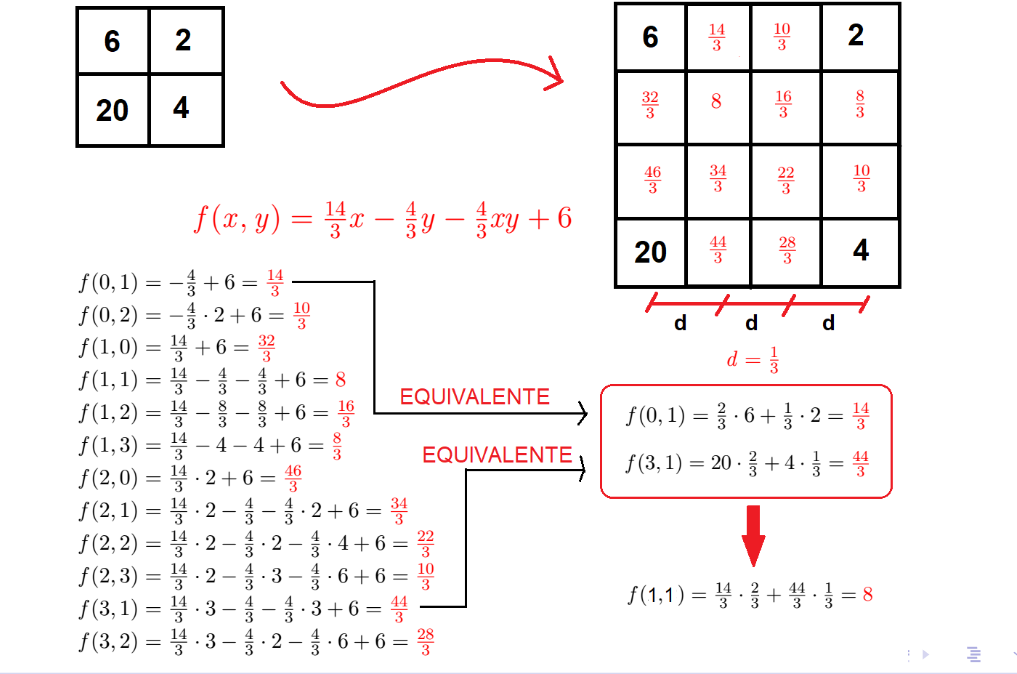
\includegraphics[width=10cm, keepaspectratio]{capitoli/immagini/imgs/calcolo_bilineare.png}
              \caption{Esempio di svolgimento di uno zoom con interpolazione bilineare.}
          \end{figure}

    \item \textbf{Interpolazione bicubica:} prevede l'utilizzo dei sedici pixel
          più vicini per stimare l'intensità da assegnare ad ogni nuova
          locazione.

          \begin{figure}[H]
              \centering
              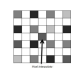
\includegraphics[width=3cm, keepaspectratio]{capitoli/immagini/imgs/interpolazione-bicubica.png}
          \end{figure}

\end{itemize}


\subsection{Shrink}

Lo stesso procedimento dello zoom, con una griglia immaginaria di dimensioni inferiori all'originale.
Per fattori interi si procede come nel caso dello zoom, ma per cancellazione di righe e colonne.

\begin{figure}[H]
    \centering
    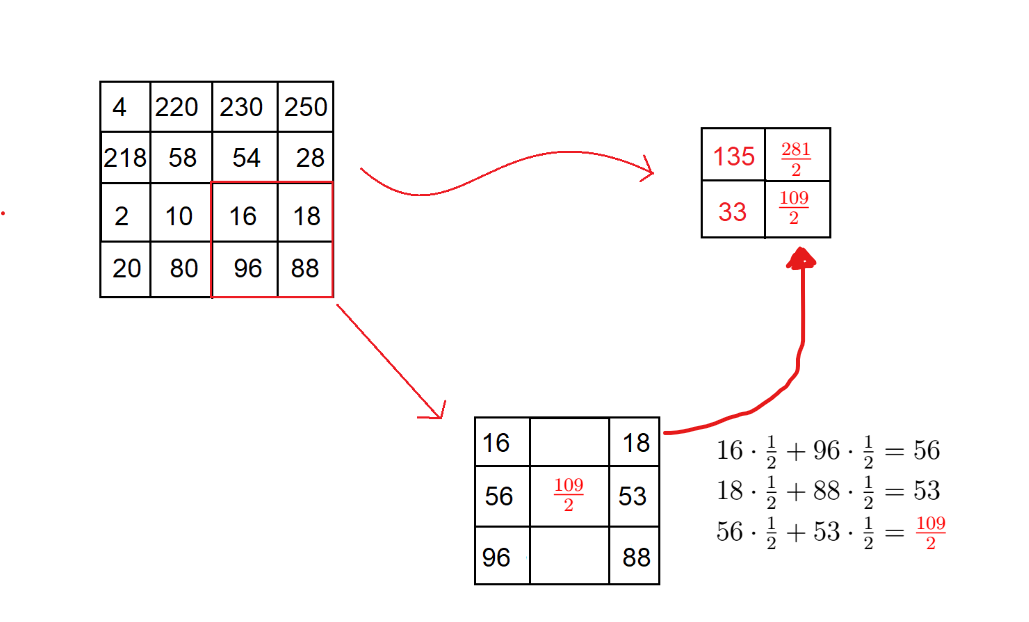
\includegraphics[width=10cm, keepaspectratio]{capitoli/immagini/imgs/calcolo_shrink.png}
    \caption{Esempio di svolgimento di uno shrink.}
\end{figure}

\section{Elaborazioni Puntuali}

\begin{definition}
    Un'elaborazione puntuale si dice \textbf{omogenea} se il risultato
    dipende solo dal valore (in scala di grigi) del pixel a cui è applicata.\\
    Se invece il risultato dipende anche dalla posizione del pixel,
    l'elaborazione puntuale è \textbf{non omogenea}.
\end{definition}

\paragraph{Note:}

\begin{itemize}
    \item Elaborazioni puntuali sono anche dette \textbf{manipolazioni della scala dei
              grigi}\\
          Un'elaborazione puntuale omogenea può essere rappresentata da
          una trasformazione

          $$
              s = T(r)
          $$

          dove:
          \begin{itemize}
              \item $r$ è il livello di grigio dell'immagine di ingresso
              \item $s$ è il livello di grigio dell'immagine in uscita
          \end{itemize}
    \item In base al tipo di funzione T si ottiene un tipo diverso di
          trasformazione: a \textbf{gradino (threshold)}, a \textbf{rampa},
          \textbf{lineare} a \textbf{tratti},...

          \begin{figure}[H]
              \centering
              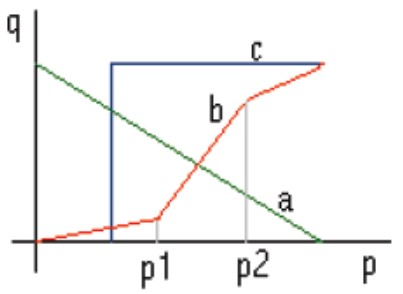
\includegraphics[width=5cm, keepaspectratio]{capitoli/immagini/imgs/elaborazioni_puntuali_immagine.jpg}
          \end{figure}

\end{itemize}

\subsection{Thresholding}

Consideriamo una funzione T a gradino, ottenendo così una
\textbf{elaborazione threshold (soglia)}.\\
Tale elaborazione fa sì che i valori dei pixel che non superano la
soglia fissata vengano portati a 0, mentre i valori dei pixel che
superano la soglia siano posti pari a 1.\\
Si produce così un'immagine \textbf{binaria}.

\begin{figure}[H]
    \centering
    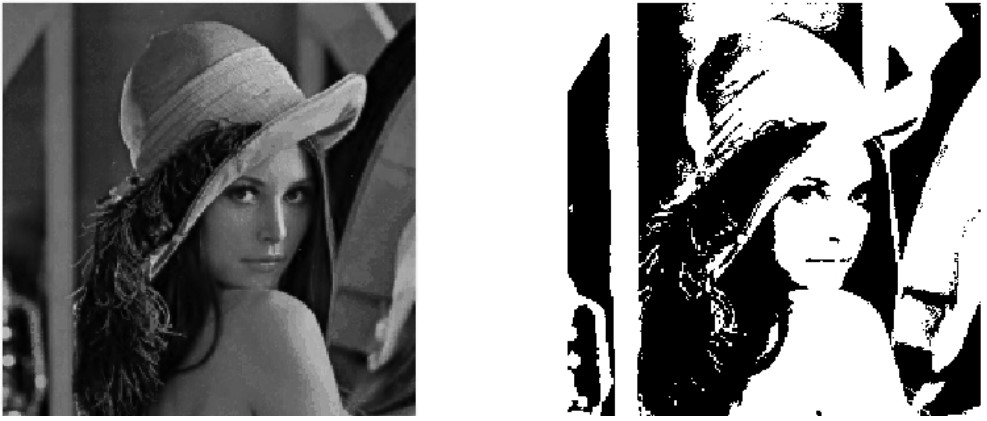
\includegraphics[width=10cm, keepaspectratio]{capitoli/immagini/imgs/foto_esempio_1.jpg}
\end{figure}

Questo è un tipico esempio di \textbf{binarizzazione}.
Si può ottenere una binarizzazione anche scegliendo una qualsiasi
altra \textbf{funzione di discriminazione}, invece di una soglia costante.

\subsection{Stiramento}

Consideriamo una $T$ del tipo:

\begin{figure}[H]
    \centering
    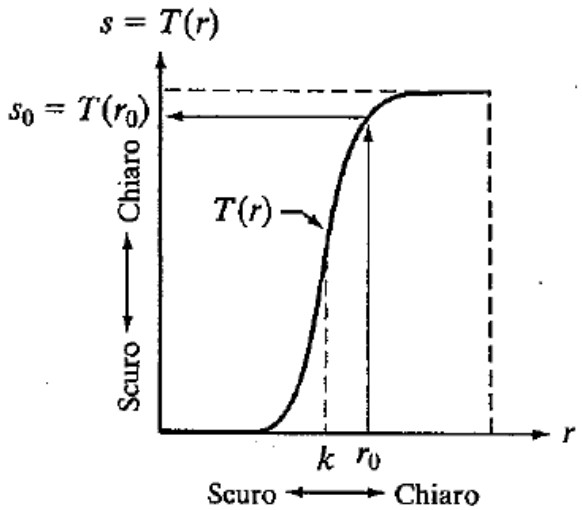
\includegraphics[width=6cm, keepaspectratio]{capitoli/immagini/imgs/trasformazione_esempio_2.jpg}
\end{figure}

Vengono scuriti i livelli di grigio al di sotto di $k$ e schiariti quelli al
di sopra di $k$. Si ottiene così uno \textbf{stiramento dell'immagine (image
    stretching)}. L'elaborazione threshold può essere riguardata come
caso limite di questo tipo di operazione.

\subsection{Negazione}

Consideriamo una $T$ del tipo:

$$
    T(r) = L - 1 - r
$$

se il range dinamico dell'immagine è $[0, L - 1]$
la scala di grigi viene invertita, ottenendo così una negazione.

\begin{figure}[H]
    \centering
    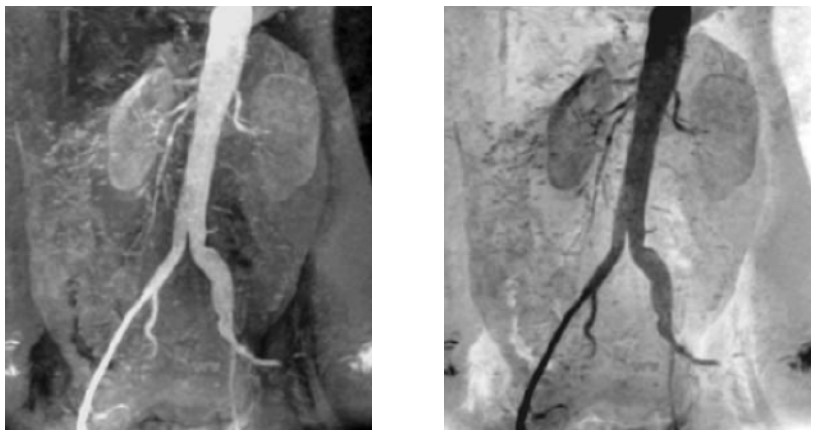
\includegraphics[width=8cm, keepaspectratio]{capitoli/immagini/imgs/angiografie_esempio_3.jpg}
\end{figure}

\subsection{Trasformazione Logaritmica}

Consideriamo una $T$ del tipo:

$$
    T(r) = c \log(1 + r), \ c \in  \mathbb{R}, r \geq 0
$$

che prende il nome di \textbf{trasformazione logaritmica}: associa ad una
stretta gamma di valori a bassa intensità dell'immagine originale
una più ampia gamma nell'immagine in output.\\
Per livelli ad alta intensità, invece, si verifica il contrario.\\
Un tipico caso in cui è utile applicare questa trasformazione è per
rappresentare la trasformata di Fourier, che spesso presenta una
gamma molto ampia di intensità, difficilmente riproducibile senza
perdere un significativo livello di dettaglio

\begin{figure}[H]
    \centering
    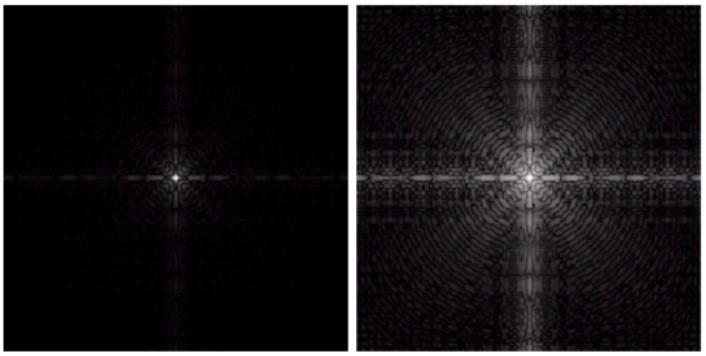
\includegraphics[width=10cm, keepaspectratio]{capitoli/immagini/imgs/trasformazione_logaritmica_esempio_4.jpg}
    \caption{Nella figura sinistra viene mostrato lo spettro di Fourier con valori in $[0, 1.5 \times 10^6]$. Mentre in quella di destra il risultato dell'applicazione della trasformazione logaritmica
        con $c = 1$ (valori in $[0, 6.2]$).
    }
\end{figure}

\subsection{Trasformazione di Potenza}

Consideriamo una $T$ del tipo:

$$
    T(r) = cr^\gamma, c, \gamma > 0,
$$

che prende il nome di \textbf{trasformazione di potenza (gamma)}
Se $\gamma < 1$ le curve potenza corrispondenti trasformano una stretta
gamma di valori scuri in una gamma più ampia di valori in output,
mentre se $\gamma > 1$, si verifica la trasformazione opposta.\\
La correzione tramite il fattore $\gamma$ è importante per la corretta
visualizzazione di immagini sullo schermo di un computer:
immagini non corrette nel modo giusto possono apparire sbiadite o,
al contrario, troppo scure.

\begin{figure}[H]
    \centering
    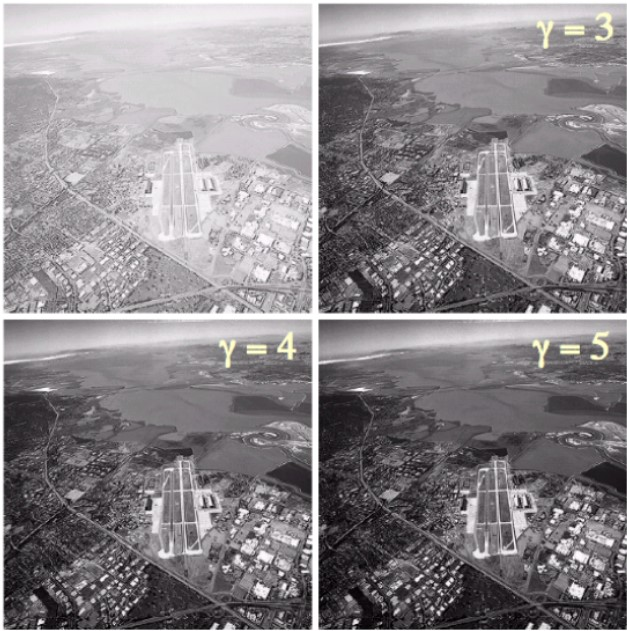
\includegraphics[width=6cm, keepaspectratio]{capitoli/immagini/imgs/foto_esempio_5.jpg}
\end{figure}

\subsection{Lineare a Tratti}

Considerando una $T$ \textbf{lineare a tratti} del tipo si ottiene uno
stretching del contrasto

\begin{figure}[H]
    \centering
    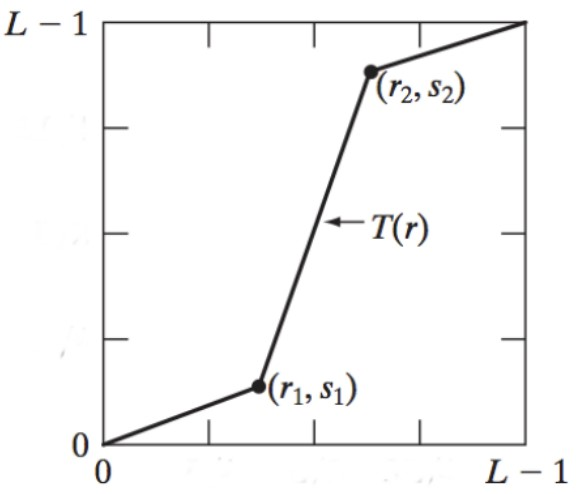
\includegraphics[width=5cm, keepaspectratio]{capitoli/immagini/imgs/lineare_a_tratti_esempio_6.jpg}
\end{figure}

In questo caso invece si ha uno stretching del contrasto differente perché si
sceglie come $(r_1, s_1) = (r_{min}, 0)$ e $(r_2, s_2) = (r_{max} , L - 1)$

\begin{figure}[H]
    \centering
    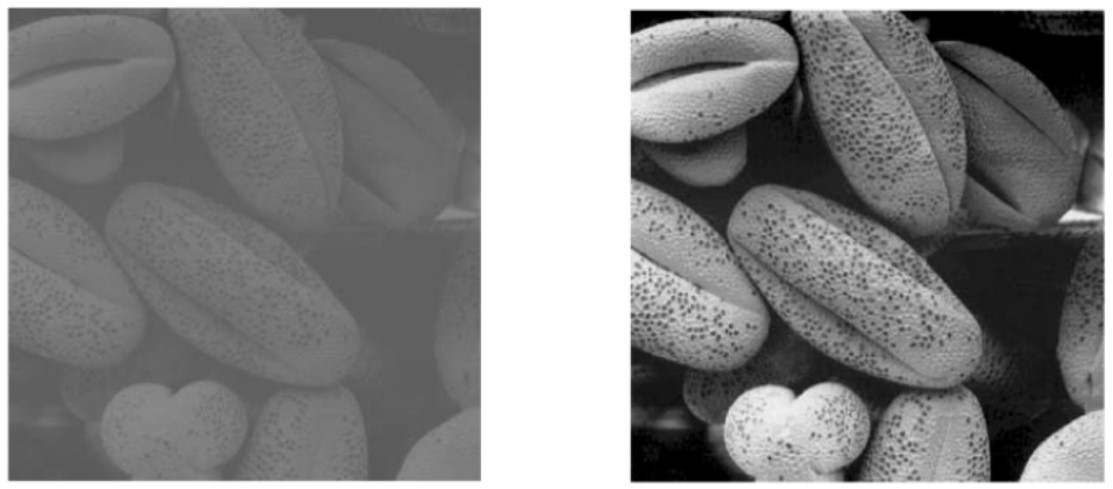
\includegraphics[width=10cm, keepaspectratio]{capitoli/immagini/imgs/globuli_rossi.jpg}
\end{figure}

\paragraph{Note:}
\begin{itemize}
    \item In questo caso $r_{min}$ e $r_{max}$ stanno ad indicare il più basso e alto valore
          nei livelli di grigio dell'immagine utilizzata.
\end{itemize}

\subsection{Altre Trasformazioni a Tratti}

\begin{figure}[H]
    \centering
    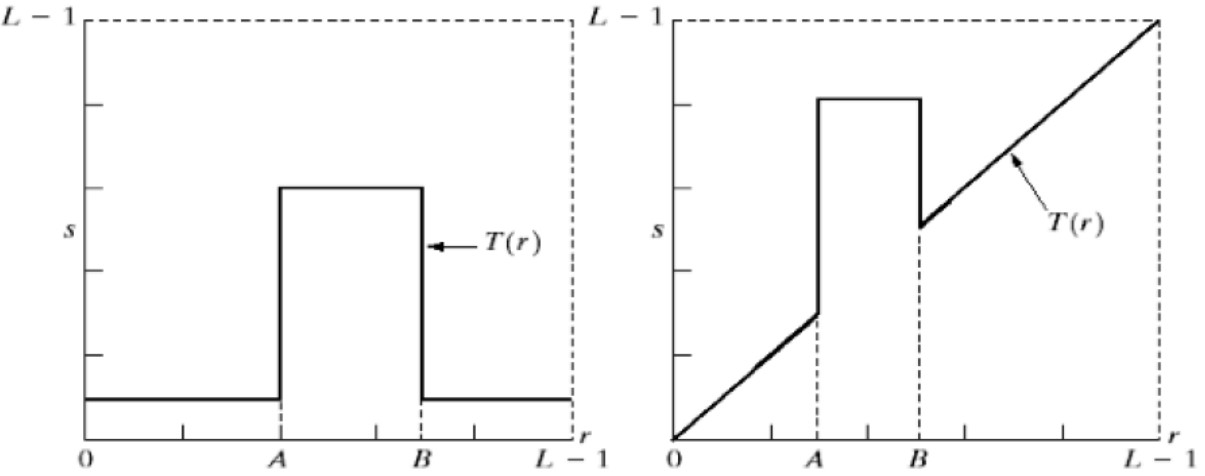
\includegraphics[width=\linewidth, keepaspectratio]{capitoli/immagini/imgs/trasformazioni_lineari_esempio_7.jpg}
\end{figure}

In questo caso prendiamo queste due diverse trasformazioni ed analizziamo il
loro effetto sull'immagine.

\begin{itemize}
    \item La prima crea una binarizzazione ma in questo caso utilizza due
          differenti gradazioni di grigio e sono precisamente bianco e nero.
    \item La seconda mette in \textbf{risalto} una porzione della scala di grigi
          alzandogli il livello e schiarendoli.
\end{itemize}

\begin{figure}[H]
    \centering
    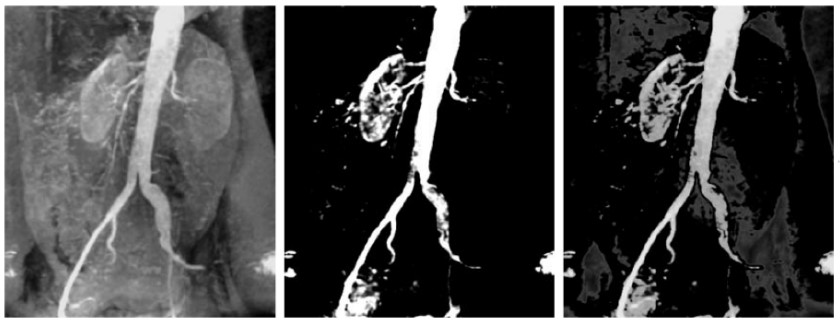
\includegraphics[width=\linewidth, keepaspectratio]{capitoli/immagini/imgs/angiografie_esempio_7.jpg}
\end{figure}

\begin{itemize}
    \item Nella prima immagine vediamo una normale Angiografia aortica.
    \item Nella seconda abbiamo il risultato della selezione di intensità del primo tipo (banda di
          interesse $[A, B]$ selezionata sulla parte alta della scala di grigi).
    \item Nella terza abbiamo il risultato della selezione di intensità del secondo tipo (banda
          $[A, B]$ sulle tonalità medio-grigie impostata sul nero, così da
          preservare le tonalità di grigio dei vasi e dei reni).
\end{itemize}

\subsection{Finestramento - Windowing}

\begin{definition}
    \textbf{Il windowing} consiste nel mostrare solo una parte del range dei valori di grigio dell'immagine.
\end{definition}

\begin{figure}[H]
    \centering
    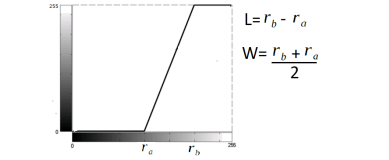
\includegraphics[width=\linewidth, keepaspectratio]{capitoli/immagini/imgs/win1.png}
\end{figure}

\textbf{Applicazione:} in molte immagini mediche il numero di valori della
scala dei grigi utili dal punto di vista diagnostico è sensibilmente
minore di tutti quelli disponibili. Usando sul monitor tutto il range
possibile si diminuisce il contrasto visibile nella zona di interesse.

\begin{figure}[H]
    \centering
    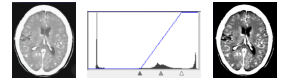
\includegraphics[width=\linewidth, keepaspectratio]{capitoli/immagini/imgs/windowing.png}
\end{figure}

\begin{itemize}
    \item Finestramento con $L = 169$ e $W = 97$
    \item Numero di grigio: $238$ (Immagine di sx) e $97$ (immagine di dx)
    \item Non viene aggiunta informazione, si aumenta solo il contrasto visibile
\end{itemize}

\section{Modelli delle Immagini}

In base al tipo di elaborazione che si vuole effettuare, può essere conveniente adottare diversi modelli per le immagini. Ad esempio:

\begin{itemize}
    \item \textbf{Modello Deterministico}
    \item \textbf{Modello Probabilistico}:
          \begin{itemize}
              \item sui \textbf{pixel} prevedendo che il loro valore sia
                    considerato una variabile aleatoria,
              \item sull'\textbf{immagine} riguardando cioè l'immagine stessa
                    come un processo stocastico

          \end{itemize}
\end{itemize}

\subsection{Il modello Probabilistico}

Nel modello probabilistico per i pixel, i valori assunti nei vari pixel ($N$ x
$M$) di un'immagine vengono considerati come valori assunti da una variabile
aleatoria in una successione di $N$ x $M$ esperimenti. Vado quini a modificare i
pixel in base ad un valore di probabilità. \\È dunque possibile analizzare ed
elaborare l'immagine utilizzando gli strumenti del calcolo delle probabilità e
del calcolo stocastico. Un esempio di questo processo è \textbf{l'analisi
    dell'istogramma}.

\subsubsection{L'istogramma dei toni di grigio}

\begin{definition}
    L'istogramma dei toni di grigio si ottiene contando, per ogni valore del
    codominio dell'immagine (spazio di tutti i valori che possono essere assunti
    dai pixel), il numero di volte che tale valore compare nell'immagine.
\end{definition}

Il grafico che si ricava è un istogramma, cioè un grafico a barre dove l'asse delle ascisse è suddiviso in tanti punti quanti sono i
possibili toni di grigio dell'immagine.\\

In termini probabilistici, l'istogramma rappresenta la distribuzione di probabilità della variabile
aleatoria $r$ ed indica il valore di grigio di un pixel, e quindi può essere visto come
la \textbf{carta d'identità di un'immagine}. Saper leggere l'istogramma ci
da un valore \textbf{qualitativo} dell'Immagine.

\begin{trivlist}
    \item \textbf{Esempio}: il codominio di un'immagine a 256 toni di grigio sarà formato da tutti i numeri interi da 0 a 255 $\rightarrow$ l'asse orizzontale sarà suddiviso in 256 parti.
\end{trivlist}

\begin{figure}[H]
    \centering
    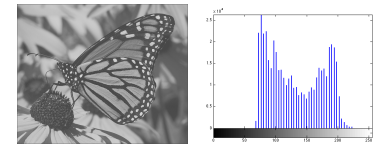
\includegraphics[width=\linewidth, keepaspectratio]{capitoli/immagini/imgs/esempio-istogramma.png}
\end{figure}

\begin{definition}
    In base alla definizione di distribuzione l'istogramma andrebbe normalizzato
    in modo da assumere valori tra 0 e 1. Se i toni di grigio sono $r_k$, $k =
        0, \ldots, 255$ allora l'altezza della barra in $r_k$ è pari alla frequenza
    relativa di $r_k$, ovvero:

    $$
        p(r_k) = \frac{n_k}{n}
    $$

    dove $n_k$ è il numero di pixel in cui viene assunto $r_k$, $n$ è il numero
    totale di pixel dell'immagine.
\end{definition}

L'istogramma quindi fornisce una raffigurazione sintetica del contenuto cromatico o di luminosità dell'immagine, dunque una descrizione
della qualità dell'immagine.

\begin{itemize}
    \item \textbf{Immagine troppo scura}
          la distribuzione è concentrata su toni bassi di grigio

          \begin{figure}[H]
              \centering
              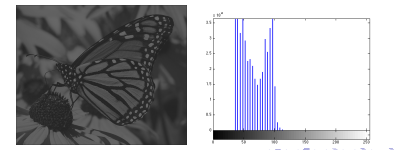
\includegraphics[width=\linewidth, keepaspectratio]{capitoli/immagini/imgs/isto-scuro.png}
          \end{figure}

    \item \textbf{Immagine troppo chiara}
          la distribuzione è concentrata su toni alti di grigio

          \begin{figure}[H]
              \centering
              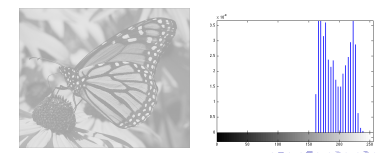
\includegraphics[width=\linewidth, keepaspectratio]{capitoli/immagini/imgs/isto-chiaro.png}
          \end{figure}

    \item \textbf{Immagine con alto contrasto}
          la distribuzione è concentrata su valori vicini a 0 e a 255. L'alto contrasto dell'immagine è quindi dovuto all'uniformità dell'istogramma.

          \begin{figure}[H]
              \centering
              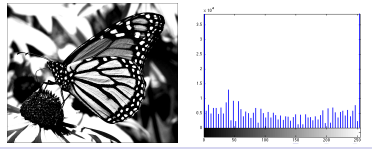
\includegraphics[width=\linewidth, keepaspectratio]{capitoli/immagini/imgs/alto-c.png}
          \end{figure}
\end{itemize}

\subsubsection{Interventi sull'istogramma}

Qualora le caratteristiche della distribuzione dei toni di grigio nell'immagine non siano ottimali, è consigliabile applicare
all'istogramma opportune trasformazioni, basate su sistemi stocastici.
\\Tra queste:

\paragraph{Equalizzazione dell'istogramma}

\begin{definition}
    Ha lo scopo di uniformare l'istogramma dell'immagine lungo tutto
    il suo dominio.
\end{definition}
Il risultato è un nuovo istogramma in cui il numero di pixel ad ogni
tono di grigio è il più possibile costante. \\\\
\textbf{Algoritmo:}

$$
    T(r_k) = (L-1)\sum_{j=0}^{k}p(r_j)=\frac{L-1}{n} \sum_{j=0}^{k}n_j = \frac{L-1}{MN}\sum_{j=0}^{k}n_j
$$

con $k=0,...,L-1$.
\\\\
\textbf{Il risultato} è l'aumento del contrasto.

\begin{figure}[H]
    \centering
    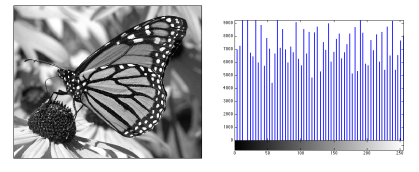
\includegraphics[width=\linewidth, keepaspectratio]{capitoli/immagini/imgs/eq-istogramma.png}
    \caption{L'immagine mostra il risultato dell'equalizzazione dell'istogramma.}
\end{figure}
\paragraph{Shift dell'istogramma}

\begin{definition}
    Lo Shift dell'istogramma consiste nel traslare i valori dell’istogramma.
\end{definition}
\textbf{Algoritmo:}

\begin{center}
    $T(r) = \alpha r$  $ \ \ \ \  0 < \alpha < 1$
    \\
    $T(r) = \alpha r + (L-1)(1-\alpha)$ $\ \ \ \ 0<\alpha<1$
\end{center}

Andrò quindi a shiftare verso sinistra o verso destra l'istogramma schiarendo o scurendo la mia immagine.
\\\\
Il \textbf{risultato} è un immagine più scura o schiarita.

\begin{figure}[H]
    \centering
    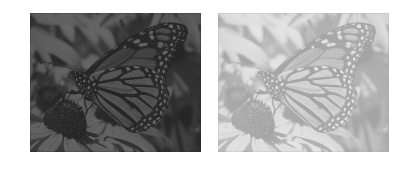
\includegraphics[width=\linewidth, keepaspectratio]{capitoli/immagini/imgs/shift-isto.png}
    \caption{L'immagine mostra il risultato dello Shift dell'isogramma.}
\end{figure}

\paragraph{Stretching dell'istogramma}

\begin{definition}
    Lo Stretching dell'istogramma consiste in uno $stiramento$ dell'istogramma, in modo da distanziarne i picchi.
\end{definition}

Si usa quando l'istogramma presenta dei picchi abbastanza ravvicinati, provocando un'immagine
piuttosto uniforme.
\\\\
\textbf{Algoritmo:}

$$
    T(r) =
    \begin{cases}
        0,                                         & 0 \le r \le r_{min}       \\
        (r - r_{min}) \frac{L-1}{r_{max}-r_{min}}, & r_{min} \le r \le r_{max} \\
        L-1,                                       & r_{max} \le r \le L-1
    \end{cases}
$$

dove $[r_{min}, r_{max} ]$ è il range osservato nell'immagine originale,
individuato dal minimo e dal massimo livello di grigio che presenta l'immagine.
\\Il risultato è \textbf{l'aumento di contrasto}

\begin{figure}[H]
    \centering
    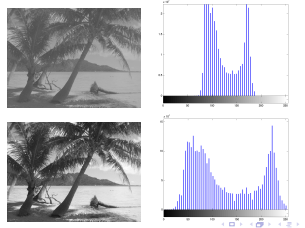
\includegraphics[width=\linewidth, keepaspectratio]{capitoli/immagini/imgs/stretch-isto.png}
\end{figure}

\section{Il Rumore}

\begin{definition}
    si intende l'insieme dei segnali indesiderati che si sovrappongono al segnale utile oggetto di studio (ad esempio un'immagine) causandone una degenerazione.
\end{definition}

Si possono avere diverse forme di degrado tra cui:
\begin{itemize}
    \item \textbf{Il rumore di quantizzazione}
    \item \textbf{Il rumore introdotto da condizioni esterne}
    \item \textbf{Il rumore introdotto dal sensore}
    \item \textbf{Il rumore introdotto dai dispositivi di
              amplificazione/condizionamento del segnale}
\end{itemize}

In base alle sue cause, il rumore si distingue tra:
\begin{itemize}
    \item \textbf{Rumore indipendente dal segnale} (additivo)
    \item \textbf{Rumore dipendente dal segnale} (la relazione tra il segnale
          corrotto e quello originale è non lineare)
\end{itemize}

\begin{trivlist}
    \item \textbf{Rumore indipendente dal segnale:} (caso più comune) la funzione
    che descrive il segnale corrotto è:

    $$
        f(x,y) = g(x,y)+v(x,y)
    $$
    dove $g(x,y)$ è il segnale e $v(x,y)$ è il rumore, che sarà di tipo
    \textbf{additivo}

    \item \textbf{Rumore dipendente dal segnale:} l'intensità del rumore dipende
    dal segnale. Supponendo anche che esso sia molto più grande del segnale, la
    funzione è

    $$
        f(x,y)=g(x,y)+v(x,y)g(x,y)=g(x,y)(1+v(x,y)) \approx g(x,y)v(x,y)
    $$

    dove $g(x,y)$ è il segnale e $v(x,y)$ è il rumore, che sarà di tipo
    \textbf{moltiplicativo}
\end{trivlist}

Essendo di natura intrinsecamente stocastica, il rumore viene in genere analizzato usando la teoria dei processi stocastici ed è
caratterizzato in base alla:

\begin{itemize}
    \item \textbf{Distribuzione:} descrive la probabilità che il rumore assuma
          certi valori di intensità
    \item \textbf{Distribuzione spettrale:} ha a che fare con l'energia ad esso
          associata, al variare della frequenza
\end{itemize}

\subsection{Il modello del rumore}

Per poter caratterizzare e studiare il rumore in un'immagine si fanno in genere delle ipotesi semplificative, in modo che il rumore abbia una qualche distribuzione di probabilità: si costruisce in
questo modo un modello del rumore.
\\Una modellizzazione tipica prevede che:

\begin{itemize}
    \item \textbf{lo spettro abbia distribuzione uniforme (rumore bianco)}
    \item \textbf{il rumore abbia distribuzione gaussiana, cioè}
          \begin{equation*}
              p(r)=\frac{1}{\sigma \sqrt{2 \pi}}e^{-\frac{(r-\mu)^2}{2\sigma^2}}
              \qquad
              \begin{gathered}
                  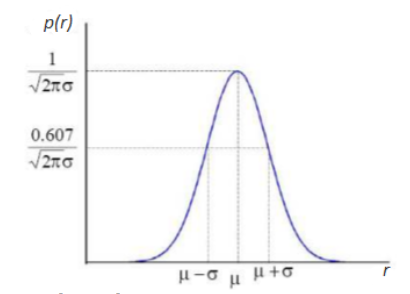
\includegraphics[width=6cm, keepaspectratio]{capitoli/immagini/imgs/campana.png}
              \end{gathered}
          \end{equation*}
          dove $\mu$ è il valor medio e $\sigma$ la deviazione standard.
\end{itemize}

\begin{figure}[H]
    \centering
    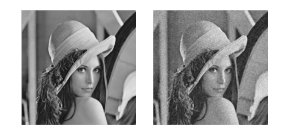
\includegraphics[width=8cm, keepaspectratio]{capitoli/immagini/imgs/esempio-rumore.png}
    \caption{Immagine originale e immagine corrotta da rumore gaussiano}
\end{figure}

\subsubsection{Il rumore Salt and Pepper}

Nel caso in cui il rumore abbia distribuzione spaziale di tipo impulsivo, si
parla di rumore salt and pepper (sale e pepe): agisce corrompendo in maniera
casuale i pixel dell'immagine, portandone il valore a $0$ (valore minimo)
oppure a $255$ (valore massimo).

\begin{equation*}
    p(r) = \begin{cases}
        p_a, & r = 0      \\
        p_b, & r = 255    \\
        0,   & altrimenti
    \end{cases}
    \qquad
    \begin{gathered}
        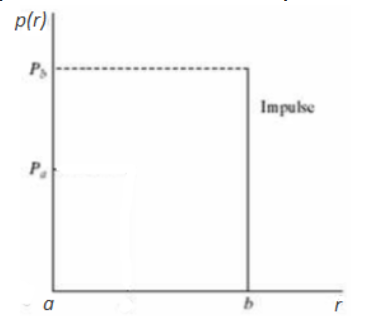
\includegraphics[width=6cm, keepaspectratio]{capitoli/immagini/imgs/salepepe.png}
    \end{gathered}
\end{equation*}

Ovviamente il rumore impulsivo, pur essendo additivo, \textbf{non è
    lineare.}

\begin{figure}[H]
    \centering
    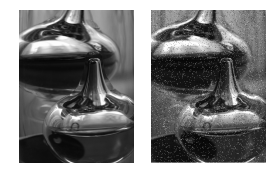
\includegraphics[width=10cm, keepaspectratio]{capitoli/immagini/imgs/esempio-salt-pepper.png}
    \caption{Immagine originale e immagine corrotta da rumore salt and pepper}
\end{figure}

\subsubsection{Rumore di Rayleigh}
Distribuzione del \textbf{rumore di Rayleigh}

\begin{equation*}
    p(r) = \begin{cases}
        \frac{2}{b}(r-a)e^{-{r-a}\frac{2}{b}}, & r \ge a \\
        0,                                     & r<a
    \end{cases}
    \qquad
    \begin{gathered}
        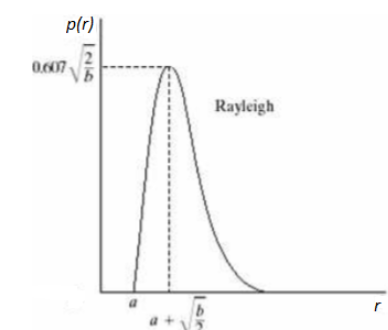
\includegraphics[width=6cm, keepaspectratio]{capitoli/immagini/imgs/raley.png}
    \end{gathered}
\end{equation*}

dove il valor medio e la deviazione standard sono dati da:

$$
    \mu = a + \sqrt{\pi b/4} \ \sigma = \sqrt{\frac{b(4-\pi)}{4}}
$$

Nel grafico lo scostamento dall'origine e la forma inclinata verso
destra rende questa densità utile per l'approssimazione di
istogrammi non simmetrici e può essere utilizzata per rappresentare
fenomeni di rumori tipici di alcuni sensori di range.

\begin{figure}[H]
    \centering
    
\includegraphics[width=8cm, keepaspectratio]{capitoli/immagini/imgs/rumore_raeli.png}
    \caption{Immagine originale e immagine corrotta da rumore Rayleigh}
\end{figure}

\subsubsection{Rumore Gamma}

Distribuzione del \textbf{rumore gamma}:

\begin{equation*}
    p(r) = \begin{cases}
        \frac{a^b r^{b-1}}{(b-1)!}e^-{ar}, & r \ge a \\
        0,                                 & r<a
    \end{cases}
    \qquad
    \begin{gathered}
        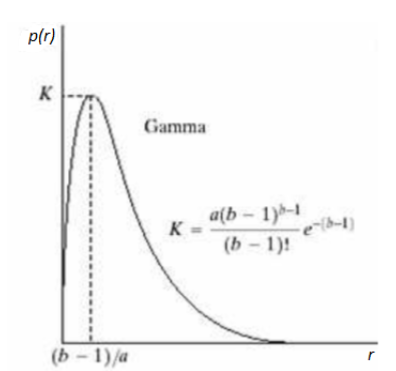
\includegraphics[width=6cm, keepaspectratio]{capitoli/immagini/imgs/gamma.png}
    \end{gathered}
\end{equation*}

dove $a > 0$, $b$ è un intero positivo e il valor medio e la deviazione standard sono dati da:

\begin{center}
    $\mu=\frac{b}{a}$ $\sigma=\frac{\sqrt{b}}{a}$
\end{center}

Questo rumore è presente nelle immagini laser.

\begin{figure}[H]
    \centering
    
\includegraphics[width=8cm, keepaspectratio]{capitoli/immagini/imgs/rumore_gamma.png}
    \caption{Immagine originale e immagine corrotta da rumore Gamma}
\end{figure}

\subsubsection{Rumore Esponenziale}

Distribuzione del \textbf{rumore Esponenziale}:

\begin{equation*}
    p(r) = \begin{cases}
        ae^{-ar}, & r \ge a \\
        0,        & r<0
    \end{cases}
    \qquad
    \begin{gathered}
        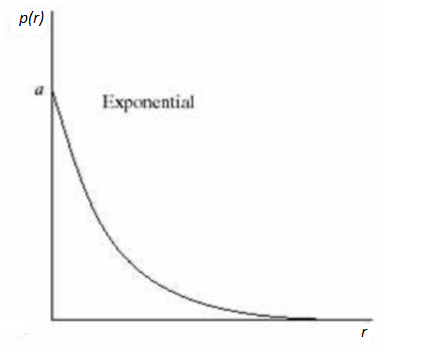
\includegraphics[width=6cm, keepaspectratio]{capitoli/immagini/imgs/esponenziale.png}
    \end{gathered}
\end{equation*}

dove $a > 0$, b e il valor medio e la deviazione standard sono dati da:

$$
    \mu = \frac{1}{a} \ \ \sigma = \frac{1}{a}
$$

Questo rumore è un caso particolare del rumore di Gamma con $b = 1$.


\begin{figure}[H]
    \centering
    
\includegraphics[width=8cm, keepaspectratio]{capitoli/immagini/imgs/esempio-esponenziale.png}
    \caption{Immagine originale e immagine corrotta da rumore Esponenziale}
\end{figure}

\subsection{Signal-Noise Ratio}

Per avere una valutazione numerica dell'entità del rumore associato ad una data immagine si può ricorrere al \textbf{rapporto segnale-rumore
    (Signal Noise Ratio - SNR)}, definito come:

\begin{center}
    $
        SNR = \frac{\sum_{(x,y)}^{}f^2(x,y)}{\sum_{(x,y)}^{}v^2(x,y)}
    $
\end{center}

dove $f(x, y)$ è l'intensità del pixel $(x, y)$ dell'immagine (già corrotta dal rumore), $v(x, y)$ è il rumore e le sommatorie sono al
variare di tutti i pixel $(x, y)$ dell'immagine.

\section{Filtri}

\begin{definition}
    Il rumore può essere corretto applicando opportune trasformazioni ai pixel dell'immagine, dette filtri.
\end{definition}
Per ogni tipo di rumore esiste un filtraggio differente, che risulterà il più
adatto ad attenuare o eliminare quel particolare rumore. In genere, la scelta
del filtro dipende dalla linearità o meno della relazione fra l'immagine
corrotta e quella originale. È possibile combinare più filtri, in modo da avere
effetti più complessi.

\subsection{Il filtraggio spaziale}

Un filtro spaziale è caratterizzato da:

\begin{itemize}
    \item Un intorno (\textbf{maschera}), in genere di dimensioni dispari;
    \item Un'operazione predefinita che viene applicata ai pixel nell'intorno
\end{itemize}
se l'operazione è lineare si parla di \textbf{filtro lineare}.
\\\\
L'intensità dell'immagine filtrata nel pixel (x,y) sarà:

\begin{center}
    $g(x,y) = \sum_{s=-a}^{a}\sum_{t=-b}^{b}w(s,t)f(x+s,y+t)$,
\end{center}

con $x=0,..,M-1$, $y=0,...,N-1$ (\textbf{correlazione di f e w}), dove i valori $w$ sono i \textbf{coefficienti della maschera}
avente dimensione $m$ x $n$, con $m = 2a+1$ e $n = 2b+1$
\\\\
Ad esempio, se la maschera ha dimensione 3 x 3, l'intensità dell'immagine filtrata nel pixel ($x,y$) sarà:
\begin{itemize}
    \item $g(x,y)=w(-1,-1)f(x-1,y-1)+w(-1,0)f(x-1,y)+...+w(0,0)f(x,y)+...+w(1,1)f(x+1,y+1)$
\end{itemize}

\subsection{Filtri lineari}

I filtri maggiormente utilizzati per la rimozione del rumore sono i cosiddetti
\textbf{filtri di smoothing}, i quali eliminano picchi e increspature
(passa-basso).

\subsubsection{Filtro medio}
Il filtro medio sostituisce il valore di ogni pixel prefissato con il
valor medio dei pixel in un suo intorno di dimensioni fissate.

\[
    \frac{1}{mn} \times
    \begin{bmatrix}
        1      & \ldots & 1      \\
        \vdots & \ddots & \vdots \\
        1      & \ldots & 1
    \end{bmatrix}
\]

Il \textbf{filtro medio} è molto utilizzato ad esempio per correggere il
\textbf{rumore gaussiano.}

\begin{figure}[H]
    \centering
    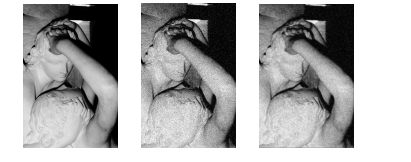
\includegraphics[width=\linewidth, keepaspectratio]{capitoli/immagini/imgs/filtro-medio-esempio2.png}
    \caption{Immagine originale, immagine corrotta da rumore gaussiano e immagine filtrata con filtro medio}
\end{figure}

\subsubsection{Filtro di media ponderata}
Il filtro media ponderata sostituisce il valore di ogni pixel prefissato con la media ponderata dei pixel in un suo
intorno di dimensioni fissate.

\begin{center}
    $g(x,y)=\frac{\sum_{s=-a}^{a}\sum_{t=-b}^{b}w(s,t)f(x+s,y+t)}{\sum_{s=-a}^{a}\sum_{t=-b}^{b}w(s,t)}$
\end{center}

\subsubsection{Filtro Gaussiano}
Il filtro gaussiano: sostituisce al valore di ogni pixel prefissato la
media pesata dei valori dei pixel in un suo intorno. I pesi sono distribuiti secondo una funzione gaussiana.

\[
    \frac{1}{16} \times
    \begin{bmatrix}
        1 & 2 & 1 \\
        2 & 4 & 2 \\
        1 & 2 & 1
    \end{bmatrix}
\]

\begin{figure}[H]
    \centering
    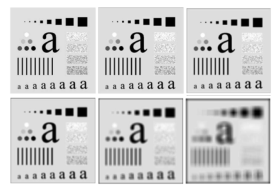
\includegraphics[width=10cm, keepaspectratio]{capitoli/immagini/imgs/filtri-l-esempio.png}
    \caption{Possiamo vedere l'applicazione della sfocatura con filtro medio
        tramite maschere di dimensioni 3, 5, 9, 15, 35 su un immagine di $500 \times 500$ pixel.}
\end{figure}

\subsection{Filtri non lineari}
I rumori non lineari (ad esempio quello impulsivo) non possono essere corretti con i filtri lineari.
Possono essere trattati invece efficacemente con \textbf{filtri non lineari}
\subsubsection{Filtro mediano}
Il filtro Mediano sostituisce al valore di ogni pixel prefissato la
mediana (valore centrale della lista ordinata) dei
valori dei pixel nell'intorno fissato.

Il filtro mediano risulta particolarmente adatto a correggere il rumore \textbf{salt and pepper}, a differenza del filtro medio che, come si
vede dall'esempio seguente, non risulta invece particolarmente efficace.

\begin{figure}[H]
    \centering
    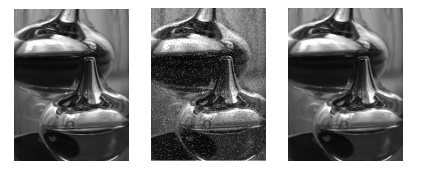
\includegraphics[keepaspectratio]{capitoli/immagini/imgs/esempio-filtro-mediano.png}
    \caption{Immagine originale, immagine corrotta da rumore \textbf{salt and pepper} e immagine filtrata con \textbf{filtro mediano}}
\end{figure}
\begin{figure}[H]
    \centering
    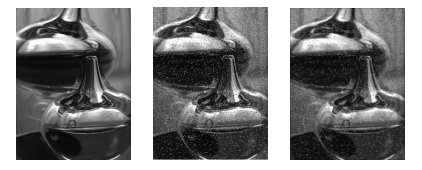
\includegraphics[keepaspectratio]{capitoli/immagini/imgs/esempio-filtro-medio.png}
    \caption{Immagine originale, immagine corrotta da rumore \textbf{salt and pepper} e immagine filtrata con \textbf{filtro medio}}
\end{figure}

\subsubsection{Filtro di massimo}

Sia $S_p$ una maschera di dimensioni $m $ x $n$, dove $p = (x,y)$ è il pixel centrale della maschera.
Il filtro di massimo sostituisce a p il massimo dei valori dei pixel in $S_p$, cioè

$$
    g_{max}(x,y)= \max_{(x,y) \in S_p} f(x,y)
$$

Questo filtro è utile per \textbf{diminuire il rumore di tipo "pepper"}.

\subsubsection{Filtro di minimo}

Il \textbf{filtro di minimo} sostituisce a $p$ il minimo dei valori dei pixel in $S_p$ cioè:

$$
    g_{min}(x,y) = \min_{(x,y) \in S_p} f(x,y)
$$

Questo filtro è utile \textbf{per diminuire il rumore di tipo "salt"}

\subsubsection{Filtro di Punto Medio}

Il filtro di punto medio sostituisce a $p$ il punto medio tra il massimo ed il minimo
dei valori dei pixel in $S_p$, cioè

$$
    g(x,y) = \frac{1}{2} \left[\max_{(x,y) \in S_p} f(x) + \min_{(x,y) \in S_p} f(x)\right]
$$

\subsubsection{Filtro medio alpha-trimmed}

Fissato un valore $0 \le d \le mn - 1$, supponiamo di cancellare in $S_p$ i $d/2$ valori più chiari e i $d/2$ valori più scuri; delle
restanti intensità ne calcoliamo la media aritmetica, cioè:

$$
    g(x,y) = \frac{1}{mn-d} \sum_{(x,y) \in \bar{S_p}} f(x,y)
$$

dove $\bar{S_p}$ è l'insieme dei pixel $S_p$ rimanenti.
Questo filtro risulta utile in situazioni in cui \textbf{si sovrappongono diversi tipi di rumore}, ad esempio nel caso di una combinazione tra
rumore salt an pepper e rumore gaussiano.

\section{Filtri di Sharpening}

L'obiettivo di questi filtri è quello di \textbf{marcare i bordi (edge
    detection)}, attribuendo meno importanza alle aree che hanno variazione lenta a
livello di intensità. Si basano sull'operatore di derivazione ed hanno l'effetto
di evidenziare soltanto i bordi dell'immagine. In forma discreta, se $f$
rappresenta l'intensità associata a ogni pixel $(x,y)$, le derivate possono
essere espresse come differenze finite:

\begin{center}
    $\frac{\partial{f}}{\partial{x}}(x,y) \sim f(x+1, y) - f(x, y)$, $\frac{\partial{f}}{\partial{y}}(x,y) \sim f(x,y+1) - f(x,y)$
    \\
    $\frac{\partial{f^2}}{\partial{x^2}}(x,y) \sim f(x+1,y) + f(x-1, y) - 2f(x,y)$
    \\
    $\frac{\partial{f^2}}{\partial{y^2}}(x,y) \sim f(x,y+1) + f(x, y-1) - 2f(x,y)$
\end{center}

Il filtro di sharpening ha l'effetto di evidenziare soltanto i bordi dell'immagine.
\begin{figure}[H]
    \centering
    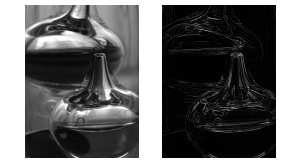
\includegraphics[width=8cm, keepaspectratio]{capitoli/immagini/imgs/sharpening.png}
    \caption{Applicazione di un filtro di sharpening}
\end{figure}

\TODO[inline]{Da ricontrollare e aggiungere spiegazioni}
\begin{figure}[H]
    \centering
    \includegraphics[width=11cm, keepaspectratio]{capitoli/immagini/imgs/sharpering2.png}
\end{figure}

\subsection{Filtro del Gradiente}

Operatore Gradiente:

\begin{center}
    $\nabla f=(\frac{\partial{f}}{\partial{x}}, \frac{\partial{f}}{\partial{y}})$,
\end{center}

Una comune implementazione della derivata prima nell'ambito dell'image processing è costituita dal modulo del gradiente

\begin{center}
    $| \nabla f(x,y) |$ $\sim$ $|\frac{\partial{f}}{\partial{x}}|$ $+$ $|\frac{\partial{f}}{\partial{y}}|$
\end{center}

Maschere:

\begin{center}
    \[
        \begin{bmatrix}
            0 & 0  & 0 \\
            0 & -1 & 0 \\
            0 & 1  & 0
        \end{bmatrix}
        \begin{bmatrix}
            0 & 0  & 0 \\
            0 & -1 & 1 \\
            0 & 0  & 0
        \end{bmatrix}
    \]
\end{center}

\begin{figure}[H]
    \centering
    \includegraphics[width=8cm, keepaspectratio]{capitoli/immagini/imgs/gradiente.png}
    \caption{Applicazione del Filtro del Gradiente}
\end{figure}

\subsection{Filtro di Sobel}
Un'altra approssimazione discreta del gradiente è data da:

\begin{align*}
    \nabla f(x,y) & \sim \frac{\partial{f}}{\partial{x}} + \frac{\partial{f}}{\partial{y}} \sim \\
                  & \sim  |[f(x+1,y-1) + 2f(x+1,y) + f(x+1 y+1)]  \ +                           \\
                  & - |[f(x-1, y-1)+2f(x-1,y) + f(x-1, y+1)]|     \ +                           \\
                  & + |[f(x-1, y+1) + 2f(x,y+1)+f(x+1,y+1)]       \ +                           \\
                  & - [f(x-1,y -1) + 2f(x,y-1) + f(x+1,y-1)]|
\end{align*}

Maschere:

\begin{center}
    \[
        \begin{bmatrix}
            -1 & -2 & -1 \\
            0  & 0  & 0  \\
            1  & 2  & 1
        \end{bmatrix}
        \begin{bmatrix}
            -1 & 0 & 1 \\
            -2 & 0 & 2 \\
            -1 & 0 & 1
        \end{bmatrix}
    \]
\end{center}

che sono detti \textbf{operatori di Sobel.}

\begin{figure}[H]
    \centering
    \includegraphics[width=8cm, keepaspectratio]{capitoli/immagini/imgs/sobel.png}
    \caption{Immagine originale e immagine filtrata tramite il gradiente di Sobel.}
\end{figure}

\subsection{Filtro di Prewitt}
Analogo a quello di Sobel eccetto per le maschere di convoluzione
che in questo caso sono:
\begin{center}
    \[
        \begin{bmatrix}
            -1 & 0 & 1 \\
            -1 & 0 & 1 \\
            -1 & 0 & 1
        \end{bmatrix}
        \begin{bmatrix}
            -1 & -1 & -1 \\
            0  & 0  & 0  \\
            1  & 1  & 1
        \end{bmatrix}
    \]
\end{center}


\begin{figure}[H]
    \centering
    \includegraphics[width=8cm, keepaspectratio]{capitoli/immagini/imgs/prewitt.png}
    \caption{Immagine originale e immagine filtrata tramite il gradiente
        di Prewitt.}
\end{figure}

\subsection{Filtro di Roberts}
Si ottiene mediante la seguente approssimazione del gradiente:

\begin{align*}
    |\nabla f(x,y)| & \sim |\frac{\partial{f}}{\partial{x}}| + |\frac{\partial{f}}{\partial{y}}| \sim \\
                    & \sim |f(x,y) - f(x+1, y+1)| + |f(x+1, y) - f(x,y+1)|
\end{align*}

Calcola il gradiente lungo le direzioni diagonali.
\\\\
Maschere:

\begin{center}
    \[
        \begin{bmatrix}
            0 & 0 & 0  \\
            0 & 1 & 0  \\
            0 & 0 & -1
        \end{bmatrix}
        \begin{bmatrix}
            0 & 0 & 0  \\
            0 & 0 & -1 \\
            0 & 1 & 0
        \end{bmatrix}
    \]
\end{center}

\begin{figure}[H]
    \centering
    \includegraphics[width=10cm, keepaspectratio]{capitoli/immagini/imgs/roberts.png}
    \caption{Nella figura possiamo osservare l'applicazione delle singole matrici $\nabla x$, $\nabla y$ e poi l'applicazione di tutte e due in contemporanea (filtro di Roberts).}
\end{figure}

\subsection{Filtro Laplaciano}

Operatore Laplaciano:

\begin{align*}
    \nabla^2 f & = \frac{\partial^2{f}}{\partial{x^2}} + \frac{\partial^2{f}}{\partial{y^2}} \sim \\
               & \sim f(x+1,y)+f(x-1,y)+f(x,y+1)+f(x,y-1)-4f(x,y)
\end{align*}

Maschera:

\begin{center}
    \[
        \begin{bmatrix}
            0 & 1  & 0 \\
            1 & -4 & 1 \\
            0 & 1  & 0
        \end{bmatrix}
    \]
\end{center}

oppure, tenendo conto delle direzioni diagonali:

\begin{center}
    \[
        \begin{bmatrix}
            1 & 1  & 1 \\
            1 & -8 & 1 \\
            1 & 1  & 1
        \end{bmatrix}
    \]
\end{center}

\begin{figure}[H]
    \centering
    \includegraphics[width=8cm, keepaspectratio]{capitoli/immagini/imgs/laplaciano.png}
    \caption{(a) Immagine originale, (b) con laplaciano, (c) con laplaciano con
        diagonali.}
\end{figure}

\subsection{Filtro Differenziale}

Sfrutta la proprietà di attraversamento dello zero della derivata seconda nelle varie direzioni, coordinate e diagonali, che ha come effetto quello di evidenziare direzionalmente i bordi di un'immagine lungo di esse.
\\Dalle approssimazioni:

\begin{align*}
    \frac{\partial^2{f}}{\partial{x}^2}(x,y) & \sim f(x+1,y)+f(x-1,y)-2f(x,y),                                \\
    \frac{\partial^2{f}}{\partial{y}^2}(x,y) & \sim f(x,y+1)+f(x,y-1)-2f(x,y),                                \\
    \frac{\partial^2{f}}{\partial{x,y}}(x,y) & \sim \frac{1}{4}[f(x-1,y-1)-f(x-1,y+1)-f(x+1,y-1)+f(x+1, y+1)]
\end{align*}

Si ottengono le maschere:
\begin{center}
    \[
        \begin{bmatrix}
            0 & 1  & 0 \\
            0 & -2 & 0 \\
            0 & 1  & 0
        \end{bmatrix}
        \begin{bmatrix}
            0 & 0  & 0 \\
            1 & -2 & 1 \\
            0 & 0  & 0
        \end{bmatrix}
        \begin{bmatrix}
            \frac{1}{4}  & 0 & -\frac{1}{4} \\
            0            & 0 & 0            \\
            -\frac{1}{4} & 0 & \frac{1}{4}
        \end{bmatrix}
    \]
\end{center}

\begin{figure}[H]
    \centering
    \includegraphics[width=8cm, keepaspectratio]{capitoli/immagini/imgs/digital-composing.png}
    \caption{Possiamo utilizzare il filtro differenziale per effettuare il Digital Compositing.}
\end{figure}

\section{Operazioni aritmetiche e Image Enhancement}

Date due immagini digitali $f(x,y)$ e $g(x,y)$ della stessa dimensione, si
possono definire le seguenti operazioni:

% \begin{align*}
%     s(x,y) = f(x,y) + g(x,y),
%     t(x,y) = f(x,y)-g(x,y),
%     p(x,y)=f(x,y) \cdot g(x,y),
%     d(x,y) = f(x,y)/g(x,y), (g(x,y) \neq 0, \forall(x,y)).
% \end{align*}

\begin{itemize}
    \item \textbf{Sommatoria di immagini:}
          date due immagini è possibile definire la loro somma come:

          $$
              s(x,y) = f(x,y) + g(x,y)
          $$

          Questa operazione è utile per effettuare l'enhancement con
          un'operazione di sommatoria.\\

          Siano $g_i(x,y)$ $K$ immagini corrotte da rumore additivo $\eta_i$ (eta),
          ovvero

          $$
              g_i(x,y) = f(x,y) + \eta_i(x,y), \ i=...K,
          $$

          dove $f(x,y)$ è l'immagine priva di rumore.\\
          Se $\bar{g}(x,y)$ è la loro media, ovvero

          $$
              \bar{g}(x,y)=\frac{1}{K} \sum_{i=1}^{K}g_i(x,y)
          $$

          allora sotto opportune ipotesi, risultata:

          $$
              E\left[\bar{g}(x,y)\right] = f(x,y) \ \text{ e } \ \sigma^2_{\bar{g}(x,y)}=\frac{1}{K}\sigma^2_{\eta(x,y)}
          $$

          \begin{figure}[H]
              \centering
              \includegraphics[width=10cm, keepaspectratio]{capitoli/immagini/imgs/sommatoria-immagini.png}
              \caption{a) Immagine originale affetta da rumore gaussiano
                  b)-f) Risultato della media di 5, 10, 20, 50 e 100 immagini
                  rumorose.}
          \end{figure}

    \item \textbf{Sottrazione di immagini}

          $$
              g(x,y) = f(x,y)-h(x,y)
          $$

          Si utilizza, ad esempio, quando si vogliono evidenziare le differenze
          fra due immagini, dove $h(x,y)$, detta maschera, è un'immagine della
          regione di interesse. Un esempio è la \textbf{Digital
              Subtraction Angiography (DSA)}.
          \begin{figure}[H]
              \centering
              \includegraphics[width=10cm, keepaspectratio]{capitoli/immagini/imgs/sottrazione.png}
          \end{figure}

    \item \textbf{Moltiplicazione e divisione di immagini}
          \TODO[inline]{Ricontrollare ed ampliare!}
          $$
              g(x,y) = f(x,y) \cdot h(x,y)
          $$
          \textbf{Esempi:}
          \begin{itemize}
              \item Correzzione dell'ombreggiatura(shading)
              \item Selezione di una ROI (Region of Interest)
          \end{itemize}

          \begin{figure}[H]
              \centering
              \includegraphics[width=10cm, keepaspectratio]{capitoli/immagini/imgs/moltiplicazione.png}
          \end{figure}
\end{itemize}


\chapter{Image Segmentation}

La segmentazione di un'immagine nell'elaborazione digitale è un processo di
partizione dell'immagine in regioni significative.

\begin{definition}
    E' il processo con il quale si classificano i pixel dell'immagine che hanno caratteristiche comuni: pertanto ciascun pixel in una regione
    è simile agli altri della stessa regione per una qualche proprietà o caratteristica (colore, intensità o texture).
\end{definition}

Matematicamente, il processo di segmentazione di un'immagine $f(x,y)$ in regioni
$R_1,...,R_n$ deve soddisfare le seguenti condizioni:

\begin{itemize}
    \item $\cup^n_{i=1}$ $R_i = f(x,y)$
    \item Ogni regione $R_i$ con $i=1,...,n$ è connessa;
    \item $R_i \cap R_j = \emptyset$ con $i \neq j$;
    \item Se $P(\cdot)$ è un predicato che indica la conformità di tutti i pixel
          di una regione $R_i$ ad un particolare modello della regione
          stessa, allora devono valere:
          \begin{itemize}
              \item $P(R_i) = vero$ $\forall i = 1...n$
              \item $P(R_i \cup R_j) = falso$ $\forall R_i, R_j$ regioni adiacenti
          \end{itemize}
\end{itemize}

La segmentazione dell'immagine ha molte applicazioni:

\TODO[inline]{Riorganizzare la visualizzazione delle immagini!}

\begin{figure}[H]
    \centering
    \includegraphics[width=9cm, keepaspectratio]{capitoli/immagini/imgs/biologia.png}
    \caption{Biologia}
\end{figure}

\begin{figure}[H]
    \centering
    \includegraphics[width=9cm, keepaspectratio]{capitoli/immagini/imgs/texture.png}
    \caption{Texture}
\end{figure}

\begin{figure}[H]
    \centering
    \includegraphics[width=6cm, keepaspectratio]{capitoli/immagini/imgs/medicina.png}
    \caption{Medicina}
\end{figure}


Le fondamentali metodologie di segmentazione sono:
\begin{itemize}
    \item \textbf{Thresholding Segmentation:} segmentazione mediante
          sogliatura;
    \item \textbf{Edge Segmentation:} edge based segmentation - localizzazione
          dei bordi;
    \item \textbf{Region Based Segmentation:} operatori morfologici;
    \item \textbf{Clustering Based Segmentation:} raggruppamento di oggetti
          sulla base della loro distanza reciproca;
    \item \textbf{Matching Techniques:} tecniche basate sulla conoscenza a
          priori.
\end{itemize}

\section{Thresholding Based Segmentation}

Singoli pixel dell'immagine sono catalogati come "pixel oggetto" se il loro
valore è maggiore di una certa soglia e come "pixel di sfondo" se il valore è
sotto la soglia. L'immagine binaria in uscita ha valore pari a 1 per ogni pixel
dell'oggetto e pari a 0 per lo sfondo.

\begin{trivlist}
    \item \textbf{Problema:} individuare il valore ottimo che minimizza l'errore dovuto all'oversegmentation (troppi oggetti) e
    all'undersegmentation (pochi oggetti).
    \item \textbf{Soluzione:} sogliatura locale $\rightarrow$ scelta di un valore di soglia diverso,
    adatto ad ogni regione esaminata.
\end{trivlist}

\subsection{Thresholding manuale}
\begin{itemize}
    \item Procedura supervisionata $\rightarrow$ dipendente dall'operatore
    \item Procedura NON automatica
\end{itemize}

\begin{figure}[H]
    \centering
    \includegraphics[width=9cm, keepaspectratio]{capitoli/immagini/imgs/trash-manuale.png}
\end{figure}

\subsection{Thresholding automatico basilare}

Separazione dei picchi negli istogrammi che rappresentano oggetti diversi nell'immagine.

\begin{figure}[H]
    \centering
    \includegraphics[width=8cm, keepaspectratio]{capitoli/immagini/imgs/trash-automatico-basilare.png}
\end{figure}

\textbf{Problema:} Cosa accade se le code si sovrappongono?

\begin{figure}[H]
    \centering
    \includegraphics[width=9cm, keepaspectratio]{capitoli/immagini/imgs/trash-automatico-basilare2.png}
\end{figure}

\subsection{Metodo di Otsu (1979)}

\textbf{Idea:} trovare la soglia ottimale massimizzando \textbf{la varianza
    interclasse} o, equivalentemente, minimizzando \textbf{la varianza intraclasse}.
\\\\\textbf{Vantaggi:}

\begin{itemize}
    \item procedura non parametrica;
    \item senza supervisione;
    \item automatica;
    \item facile da implementare e costo computazionale basso nel caso di
          immagine con istogramma bimodale.
\end{itemize}

\textbf{Limiti:}

\begin{itemize}
    \item è un metodo di sogliatura globale $\rightarrow$ non tiene conto delle
          piccole variazioni di livelli di grigio;
    \item si basa solamente sull'istogramma dell'immagine (e quindi sul livello
          di grigio dei pixel) e prevede che sia bimodale.
\end{itemize}

\subsubsection{Descrizione}

Si ipotizzi che un'immagine digitale di $M \times N$ pixel, abbia $L$ differenti
livelli di grigio e si indichi con $\eta_i$ il numero di pixel di intensità i.
L'istogramma normalizzato ha componenti $p_i = \eta_i/(M$ x $N)$ da cui si ha:

$$
    \sum_{i=0}^{L-1}p_i = 1, \ p_i \ge 0
$$

Ora si ipotizzi di selezionare una soglia $T(k) = k$, $0 < k < L - 1$ e di
utilizzarla come soglia sull'immagine di input ottenendo due classi $C_0$ e
$C_1$ La probabilità $\omega_0(k)$ che un pixel venga assegnato alla classe
$C_0$ è data dalla probabilità cumulativa

$$
    \omega_0(k) = \sum_{i=0}^{k}p_i,
$$

Analogamente per la classe $C_1$ si ha:

$$
    \omega_1(k) = \sum_{i=k+1}^{L-1}p_i=1-\omega_0(k)
$$

Il valore medio (valore atteso) di intensità dei pixel appartenenti a
$C_0$ è

$$
    \mu_0(k)=\frac{1}{\omega_0(k)} \sum_{i=0}^{k}ip_i
$$

Analogamente, il valore medio di intensità della seconda classe è

$$
    \mu_1(k)=\frac{1}{\omega_1(k)}\sum_{i=k+1}^{L-1}ip_i
$$

La media e la probabilità cumulativa fino al livello $k$ sono date da:

$$
    \mu(k)=\sum_{i=0}^{k}ip_i, \ \ \omega(k)=\sum_{i=0}^{k}p_i
$$

mentre la media globale, cioè l'intensità media dell'intera immagine, è

$$
    \mu_T=\mu(L)=\sum_{i=0}^{L-1}ip_i
$$

devono valere le seguenti relazioni:

\begin{itemize}
    \item $\omega_0 \mu_0 + \omega_1 \mu_1 = \mu_T$,
    \item $\omega_0 + \omega_1 = 1$
\end{itemize}

La varianza delle due classi è data da:

$$
    \sigma^2_0 = \frac{1}{\omega_0}\sum_{i=0}^{k}(i-\mu_0)^2p_i, \ \ \sigma^2_1 = \frac{1}{\omega_1}\sum_{i=0}^{k}(i-\mu_1)^2p_i
$$

La \textbf{la varianza interclasse} è definita come:

$$\sigma^2_W = \omega_0 \sigma^2_0 + \omega_1 \sigma^2_1
$$

ovvero la somma pesata delle varianze delle due classi.
\\\\Mentre la \textbf{varianza interclasse} è data da

$$
    \sigma^2_B = \omega_0(\mu_0 - \mu_T)^2 + \omega_1(\mu_1 - \mu_T)^2 = \omega_0\omega_1(\mu_1-\mu_0)^2 = \frac{\left[\mu_T \omega_k - \mu(k)\right]^2}{\omega(k)(1-\omega(k))}
$$

Da notare che $\sigma^2_B$  cresce all'aumentare della distanza tra i due valori medi $\mu_0$ e $\mu_1$, mettendo in evidenza che la varianza interclasse è la misura della separabilità tra le classi.
\\\\
La soglia ottimale è data dal valore $k^*$ che massimizza $\sigma^2_B(k)$, ovvero

$$
    \sigma^2_B(k) = \max_{0\le k \le L-1} \sigma^2_B(k)
$$

Una volta che è stato trovato $k^*$ l'immagine viene segmentata nel modo seguente:

$$
    g(x,y) = \begin{cases}
        1 & \ \text{ se } f(x,y) > k^*   \\
        0 & \ \text{ se } f(x,y) \le k^*
    \end{cases}
$$

L'algoritmo può essere riassunto come segue:

\begin{enumerate}
    \item calcolare l'istogramma normalizzato dell'immagine denotando le componenti $p_i$, $i=0,1,2,...,L-1$;
    \item calcolare la probabilità cumulativa $\omega(k)$;
    \item calcolare la media cumulativa $\mu(k)$;
    \item calcolare l'intensità media globale $\mu_T$;
    \item calcolare la varianza interclasse $\sigma^2_B$;
    \item  calcolare la soglia di Otsu $k^*$, cioè il valore di $k$ che rende massima la varianza interclasse;
\end{enumerate}

Esiste un'estensione del metodo di Otsu che prende il nome di metodo di \textbf{Phansalkar}


\begin{figure}[H]
    \centering
    \includegraphics[width=\linewidth, keepaspectratio]{capitoli/immagini/imgs/otsu.png}
    \caption{Immagine originale e immagine sogliata con l'algoritmo Otsu}
\end{figure}

\subsection{Edge-Gray Levels Histogram method (1977)}
\TODO[inline]{Da integrare!}
Testato per la prima volta su immagini
termografiche (FLIR Forward-Looking Infra Red). Sfrutta un vettore
multidimensionale di criteri piuttosto che un solo parametro
caratterizzante come il livello di grigio.

\begin{figure}[H]
    \centering
    \includegraphics[width=8cm, keepaspectratio]{capitoli/immagini/imgs/rosenfeld.png}
\end{figure}

È un metodo di segmentazione delle immagini in uno spazio bidimensionale di parametri, in cui i criteri considerati per ciascun
pixel sono da una parte il livello di grigio (grey level), dall'altra il valore ai bordi (edge value), rappresentativo nel mondo digitale del
modulo approssimato del valore puntuale del gradiente.

\begin{figure}[H]
    \centering
    \includegraphics[width=8cm, keepaspectratio]{capitoli/immagini/imgs/edgepanda.png}
\end{figure}

\section{Clustering Based Segmentation}
\subsection{Fuzzy Selection}

La Fuzzy selection seleziona tutti i pixel di un oggetto fra loro adiacenti e che abbiano un valore compreso in un certo intervallo di livelli di grigio.
Si tratta, anche in questo caso, di una selezione multiparametrica. L'algoritmo che la implementa dovrà attraversare l'immagine etichettando i vertici in base alla connettività ed ai valori relativi dei vicini.
Al termine della scansione tutti i polimini, fra loro disgiunti, saranno etichettati con label differenti.

\begin{figure}[H]
    \centering
    \includegraphics[width=6cm, keepaspectratio]{capitoli/immagini/imgs/fuzzy-selection.png}
\end{figure}

\paragraph{Note:}
\begin{itemize}
    \item \textbf{Polimini:} è definito come \textit{un insieme di quadrati che abbiano a due a due un lato in comune}. Volgarmente solo le forme del tetris.
\end{itemize}

\section{Region Based Segmentation}
\subsection{Operatori morfologici}

La parola morfologia denota comunemente lo studio della forma.
Gli operatori morfologici matematici effettuano elaborazioni dipendentemente dalla forma di un oggetto, estraendo
dall'immagine componenti utili alla rappresentazione e descrizione della forma di una regione (contorni, scheletro, ecc...).
La struttura dell'immagine viene "sondata" con un insieme di forma definibile dall'utente (elemento strutturante).
Ora analizzeremo i principali operatori morfologici.

\subsubsection{Erosione}

Sia $I$ l'immagine da analizzare ed $SE$ un elemento strutturante.
\\\\
L'erosione tra $I$ e $SE$ è definita come:

\begin{equation}\label{eq:erosione}
    I \ominus SE = \{z \ | \ (SE)_z \subset I\}
\end{equation}

dove $(SE)_z$ indica l'elemento strutturante centrato nel punto $z$.
Quando vado a fare l'erosione quindi vado ad \textbf{eliminare z}.
\\\\
Equivalentemente si usa

$$
    I \ominus SE = \{z \ | \ (SE)_z \cap I^c = \emptyset\}
$$

Quinti l'erosione fa si che il pixel, in cui $SE$ è centrato, diventi 0 se nell'intorno di quel pixel c'è almeno uno zero;

\begin{figure}[H]
    \centering
    \includegraphics[width=10cm, keepaspectratio]{capitoli/immagini/imgs/erosione-esempio.png}
\end{figure}

Nel caso in cui stiamo lavorando con un'immagine a scala di grigi l'erosione prende il minimo valore nell'elemento strutturante:

$$
    I \ominus SE = \min\{I(z) \ | \ z \in SE\}
$$


\paragraph{Note:}
\begin{itemize}
    \item Nella (\ref{eq:erosione}) si intende che l'intero kernel deve appartenere all'immagine, quindi se ho un kernel di tutti 1 e lo centro in un punto con vicinato di tutti 0, questo non appartiene all'immagine $I$.
\end{itemize}

\subsubsection{Dilatazione}

La dilatazione, detta anche addizione di Minkowsky, tra $I$ ed $SE$ è
definita come:

$$
    I \oplus SE = \{z \ | \ (SE)_z \cap I \neq \emptyset\}
$$

La formulazione appena riportata è equivalente a:

$$
    I \oplus SE = \{(z \ | \ (SE)_z \cup I) \subset I\}
$$

Quindi la dilatazione fa sì
che il pixel, in cui $SE$ è centrato, diventi 1 se nell'intorno di quel pixel
c'è almeno un 1.

\begin{figure}[H]
    \centering
    \includegraphics[width=10cm, keepaspectratio]{capitoli/immagini/imgs/dilatazione-esempio.png}
\end{figure}

Nel caso in cui stiamo lavorando con un'immagine a scala di grigi
la dilatazione prende il massimo valore nell'elemento strutturante:

$$
    I \oplus SE = \max\{I(z) \ | \ z \in SE\}
$$

%% TODO: sembra essere inutile, ricontrollare !
% \textbf{Dilatazione - Applicazione: riempimento}

% \begin{figure}[H]
%     \centering
%     \includegraphics[width=\linewidth, keepaspectratio]{capitoli/immagini/imgs/dilatazione-applicazione.png}
% \end{figure}


\subsubsection{Apertura}
L'apertura è una erosione seguita da una dilatazione, dove si considera sempre lo stesso elemento strutturante e non è commutativa.
È definita come:

$$
    I \circ SE = (I \ominus SE) \oplus SE
$$

L'effetto dell'apertura è di preservare il più possibile regioni di forma simile all'elemento strutturante, e di eliminare quelle
differenti.

\begin{figure}[H]
    \centering
    \includegraphics[width=10cm, keepaspectratio]{capitoli/immagini/imgs/apertura.png}
\end{figure}

\begin{figure}[H]
    \centering
    \includegraphics[width=10cm, keepaspectratio]{capitoli/immagini/imgs/apertura_bella.png}
\end{figure}

\subsubsection{Chiusura}

La chiusura è una dilatazione seguita da una erosione, dove si considera sempre lo stesso elemento strutturante e non è
commutativa. È definita come:

$$
    I \bullet SE = (I \oplus SE) \ominus SE
$$

L'effetto della chiusura è di chiudere gli eventuali buchi interni tenendo conto della forma dell'elemento strutturante.

\begin{figure}[H]
    \centering
    \includegraphics[width=10cm, keepaspectratio]{capitoli/immagini/imgs/chiusura.png}
\end{figure}

\begin{figure}[H]
    \centering
    \includegraphics[width=10cm, keepaspectratio]{capitoli/immagini/imgs/chiusura_bella.png}
\end{figure}

\subsubsection{Applicazioni}

E' importante osservare come la convoluzione dell'elemento strutturante modifichi l'immagine di partenza solo alla fine
dell'analisi di tutti i punti del dominio. Un esempio di applicazione degli operatori morfologici è il problema posto da Sternberg nel 1985, al fine di controllare, a
partire da una foto binaria, l'integrità dei denti degli ingranaggi prodotti in un'azienda di orologi.

\begin{figure}[H]
    \centering
    \includegraphics[width=10cm, keepaspectratio]{capitoli/immagini/imgs/orologi-esempio.png}
\end{figure}

Come primo passo è necessario riempire i “buchi” degli ingranaggi nell'immagine originale.
Si nega l'immagine di partenza $B$ ottenendo $B^c$ e si effettua un'erosione
con un $SE$ grande come i buchi centrali degli ingranaggi, ottenendo
l'immagine (b).

\begin{figure}[H]
    \centering
    \includegraphics[width=\linewidth, keepaspectratio]{capitoli/immagini/imgs/orologi2.png}
    \caption{L'immagine a sinistra (a) è l'immagine originale $B$. Quella a destra (b) è ottenuta come $B1=B^c \ominus$ hole\_ring}
\end{figure}

Si prende un $SE$ di dimensioni maggiori rispetto ai buchi degli ingranaggi di partenza e si opera una dilatazione: il risultato è
mostrato in (c). Quindi si opera un'operazione logica di OR fra B e B2 al fine di ottenere B3, figura (d)

\begin{figure}[H]
    \centering
    \includegraphics[width=\linewidth, keepaspectratio]{capitoli/immagini/imgs/orologi3.png}
    \caption*{L'immagine a sinistra (c) è ottenuta con $B2 = B1 \oplus$ hole\_mask. L'immagine a destra (d) è ottenuta con $B3 = B \text{ OR } B2$}
\end{figure}

A questo punto si può considerare un $SE$ che abbia una dimensione tale da includere soltanto i denti degli ingranaggi al suo interno,
B7 di figura (e). Tramite un'operazione di AND è facile ottenere un'immagine
binaria contenente solo i denti degli ingranaggi da analizzare (f).

\begin{figure}[H]
    \centering
    \includegraphics[width=\linewidth, keepaspectratio]{capitoli/immagini/imgs/orologi4.png}
    \caption{A sinistra l'immagine (e) $B7$ ottenuta dall'applicazione di un kernel che evidenzia solo i denti degli ingranaggi. A destra (f) l'immagine ottenuta con $Bs = B \text{ AND } B7$}
\end{figure}

Se si sceglie un SE circolare con diametro pari alla metà della distanza fra due denti successivi e se si applica una dilatazione, si
otterranno “buchi” in corrispondenza delle strutture dentate uscenti come in figura (g). Infine, un altro elemento strutturante di diametro superiore a
quello della distanza interdentale viene utilizzato per evidenziare i denti mancanti (h).

\TODO[inline]{Riscrivere caption!}
\begin{figure}[H]
    \centering
    \includegraphics[width=\linewidth, keepaspectratio]{capitoli/immagini/imgs/orologi5.png}
    \caption*{g) $B9=B8 \oplus$ Up\_spacing}
    \caption*{h) RESULT = $((B8 * B9) \oplus$ defect\_cue)$OR B9$ }
\end{figure}

\chapter{Indici di Similarità}

\section{Mean Square Error (MSE)}

Al fine di valutare matematicamente la differenza in termini di intensità fra due immagini A e B, viene introdotto il concetto di
\textbf{Errore Quadratico Medio (MSE)}.

$$
    MSE_{AB} = \sum_{i=1}^{N}\sum_{j=1}^{M}\frac{|I_A(i,j)-I_B(i,j)|^2}{NM}
$$

dove $I_A$ e $I_B$ sono le intensità dei livelli di grigio delle due immagini di dimensioni $M$ x $N$ di cui si calcola la differenza. Più il valore di questo indice è basso, minore sarà la differenza tra
le immagini sia numericamente in termini di bit, sia in termini di qualità visiva.

\section{Peak Signal to Noise Ratio (PSNR)}

Per quantificare l'entità del suddetto errore secondo un termine di paragone, viene introdotto un ulteriore indice di qualità delle
immagini. Si definisce come \textbf{Peak Signal to Noise Ratio (PSNR)}, il rapporto
tra la massima potenza ammisibile di un segnale e l'MSE.

$$
    PSNR_{AB} = 10 \log(\frac{255^2}{MSE_{AB}})
$$

Può anche essere espresso come:

\TODO[inline]{Ricontrollare se la formula seguente è vera !}
$$
    PSNR_{AB} = 20 \log(\frac{255}{\sqrt{MSE}})
$$

\chapter{Image Registration}

\begin{definition}
    La registratura d'immagini (image registration) è quel processo che permette la trasformazione di differenti insiemi di dati, presenti in diversi insiemi di coordinate, in un sistema dove ogni coordinata
    spaziale corrisponde.
\end{definition}

La registratura è necessaria per poter confrontare o integrare i dati ottenuti da diverse misure. Si prende una delle immagini come sorgente (source) e ci si
riferisce alla seconda immagine come bersaglio (target).

\begin{figure}[H]
    \centering
    \includegraphics[width=\linewidth, keepaspectratio]{capitoli/immagini/imgs/image-registration.png}
\end{figure}

Alcune possibili applicazioni di questa tecnica sono:

\begin{itemize}
    \item Rilevamento del movimento con telecamera non stazionaria

          \begin{figure}[H]
              \centering
              \includegraphics[width=10cm, keepaspectratio]{capitoli/immagini/imgs/image-registration-applicazioni.png}
          \end{figure}

    \item Ricostruzione 3D

          \begin{figure}[H]
              \centering
              \includegraphics[width=10cm, keepaspectratio]{capitoli/immagini/imgs/ricostruzione-3-d.png}
          \end{figure}
    \item Medical imaging
          \begin{figure}[H]
              \centering
              \includegraphics[width=10cm, keepaspectratio]{capitoli/immagini/imgs/medical-imaging.png}
          \end{figure}
\end{itemize}


Una classificazione dei metodi di registratura si basa su nove criteri:

\begin{enumerate}
    \item \textit{Dimensione del dominio dell'immagine:}
          si possono considerare:
          \begin{enumerate}
              \item solamente le dimensioni spaziali:
                    \begin{itemize}
                        \item 2D/2D
                        \item 2D/3D
                        \item 3D/3D
                    \end{itemize}
              \item immagini acquisite in tempi differenti, con dimensioni spaziali:
                    \begin{itemize}
                        \item 2D/2D
                        \item 2D/3D
                        \item 3D/3D
                    \end{itemize}
          \end{enumerate}
    \item \textit{Natura della registrazione:}
          \begin{itemize}
              \item \textbf{Estrinseca:}
                    I metodi estrinseci si fondano su oggetti artificiali che vengono attaccati sul paziente. Si dividono in:
                    \begin{itemize}
                        \item Invasivi
                              \begin{itemize}
                                  \item telaio stereotassico (stereotassic frame)
                                  \item marcatori a vite (screw mounted markers)
                              \end{itemize}
                        \item Non Invasivi
                              \begin{itemize}
                                  \item stampi, adattatori dentali
                                  \item marcatori su pelle
                              \end{itemize}
                    \end{itemize}
              \item \textbf{Intrinseca}
                    I metodi intrinseci si basano sul solo contenuto dell'immagine del paziente. Si dividono in:

                    \begin{itemize}
                        \item \textbf{Landmark based:} basata sui punti fiduciali: i punti di possono essere anatomici, cioè punti precisi e
                              localizzabili della morfologia dell'anatomia visibile, solitamente identificati in modo interattivo dall'utente.
                        \item \textbf{Segmentation based:} può essere \textbf{rigid model based}, dove si
                              individuano le stesse strutture anatomiche (principalmente superfici) estratte da entrambe le immagini da registrare e
                              utilizzate come unico input per la procedura di allineamento; oppure deformable model based, dove una struttura estratta
                              (principalmente superfici e curve) da un'immagine è deformata elasticamente per adattarsi alla seconda immagine
                        \item  \textbf{Voxel property based:} si basano solamente sui livelli di grigio
                              dell'immagine (metodo globale).
                    \end{itemize}
              \item \textbf{Non basata su immagini}
          \end{itemize}
    \item \textit{Tipo di Trasformazione:}
          \begin{itemize}
              \item \textbf{Rigida:} comprende solo traslazioni e rotazioni
              \item \textbf{Affine:} mappa linee parallele in linee parallele
              \item \textbf{Proiettiva:} mappa linee in linee
              \item \textbf{Elastica:} mappa linee in curve
          \end{itemize}
    \item \textit{Dominio della Trasformazione:}
          Una trasformazione è chiamata globale se è applicata all'intera immagine, locale se è applicata ad un sottoinsieme del'immagine.
    \item \textit{Interazione:}
          Fra gli algoritmi di registratura, si possono individuare tre livelli di interazione:

          \begin{itemize}
              \item \textbf{Automatica:} l'utente fornisce all'algoritmo solo i dati
                    dell'immagine ed eventualmente informazioni sull'acquisizione
                    dell'immagine.
              \item \textbf{Interattiva:} l'utente effettua personalmente la registrazione,
                    assistito da software.
              \item \textbf{Semi-autimatica:} l'utente deve inizializzare l'algoritmo, ad esempio, segmentando i dati o guidando l'algoritmo a rifiutare
                    o accettare le ipotesi di registrazione suggerite.
          \end{itemize}

    \item \textit{Procedura di ottimizzazione:}
          \begin{itemize}
              \item \textbf{Parameters computed:} i parametri che compongono la trasformazione della registrazione vengono calcolati direttamente, cioè determinato in maniera esplicita dai dati
                    disponibili
              \item \textbf{Parameters searched for:} i parametri che compongono la trasformazione della registrazione vengono ricercati, cioè
                    determinati trovando un massimo di qualche funzione definita nello spazio dei parametri.
          \end{itemize}
    \item \textit{Modalità:}
          \begin{itemize}
              \item \textbf{Monomodale:} le immagini da registrare appartengono alla
                    stessa modalità (radiografia, CT, MR, PET, SPECT, US,
                    raggi X o DSA, ecc..)
              \item \textbf{Multimodale:} le immagini da registrare derivano da due
                    diverse modalità (TC-MR, TC-PET, TC-SPECT, DSA-MR,
                    PET-MR, US-TC, raggi X-MR, ecc..).
          \end{itemize}
    \item \textit{Soggetto:}
          \begin{itemize}
              \item \textbf{Intrasubject:} tutte le immagini coinvolte nella registrazione
                    sono acquisite da un singolo paziente;
              \item \textbf{Intersubject:} la registrazione viene effettuata utilizzando due
                    immagini di diversi pazienti (o un paziente e un modello);
              \item \textbf{Atlas:} un'immagine viene acquisita da un singolo paziente e
                    l'altra immagine è in qualche modo costruita da un database
                    di informazioni su un'immagine ottenuta utilizzando l'imaging
                    di molti soggetti.
          \end{itemize}
    \item \textit{Oggetto:}
          \begin{itemize}
              \item \textbf{Testa:} cervello, occhio, denti.
              \item \textbf{Torace:} intero, cardiaco, seno.
              \item \textbf{Addome:} generale, rene, fegato.
              \item \textbf{Bacino e perineo}
              \item \textbf{Arti} generale, femorale, omero, mano
              \item \textbf{Colonna vertebrale e vertebre}
          \end{itemize}
\end{enumerate}

\TODO[inline]{Allineare e sistemare le immagini !}
\begin{figure}[H]
    \centering
    \includegraphics[width=6cm, keepaspectratio]{capitoli/immagini/imgs/dominio.png}
    \includegraphics[width=6cm, keepaspectratio]{capitoli/immagini/imgs/tipi-trasformazione.png}
\end{figure}

\chapter{Tomografia Computerizzata}

La \textbf{Tomografia Computerizzata (TC)} è una tecnica radiologica, non
invasiva, che fornisce una serie di immagini in sezione del corpo
consentendo di distinguere i vari organi e tessuti in base alla loro
densita. Effettua una misurazione dell'attenuazione di un fascio di raggi X
fatto ruotare in diverse traiettorie attraverso lo strato corporeo in studio.

\begin{figure}[H]
    \centering
    \includegraphics[width=6cm, keepaspectratio]{capitoli/immagini/imgs/tc1.png}
\end{figure}

I raggi X vengono generati dal \textbf{Tubo Radiogeno}, un tubo di vetro al
cui interno c'è il vuoto. È
formato da \textit{catodo} che emette elettroni
per effetto termoionico, e \textit{anodo}, un disco di
tungsteno ruotante. Gli elettroni vengono accelerati e, impattando
contro il disco di tungsteno, subiscono una brusca decelerazione: in
questo passaggio si producono fotoni ad elevata frequenza (\textbf{raggi
    X}), la cui energia dipenda dalla differenza di potenziale fra anodo e
catodo.

\begin{figure}[H]
    \centering
    \includegraphics[width=8cm, keepaspectratio]{capitoli/immagini/imgs/tubo.png}
\end{figure}

\section{Processo di formazione dell'immagine}

L'immagine del corpo del paziente viene creata misurando
l'attenuazione $\mu$ di un fascio di raggi X che lo attraversa. Questa
varia in modo proporzionale alla densità elettronica dei tessuti.

\begin{figure}[H]
    \centering
    \includegraphics[width=10cm, keepaspectratio]{capitoli/immagini/imgs/ossascala.png}
    \caption{Esempio di diverse densità elettroniche degli organi.}
\end{figure}

La scala di questi valori è detta \textit{Scala di Hounsfield}.
Questa scala comprende più di mille valori e quindi va normalizzata per
essere rappresentata in un'immagine a scala di grigi (valori da 0 a 255).
L'unità di Hounsfiled per il singolo tessuto è calcolata come segue:

$$
    HU(\mu) = 1000 \times \frac{\mu - \mu_{acqua}}{\mu_{acqua} - \mu_{aria}}
$$

dove $\mu$ è il coefficiente di attenuazione del tessuto di cui si vuole calcolare il valore,
$\mu_{acqua}$ è il coefficiente di attenuazione dell'acqua (0) e $\mu_{aria}$ è
quello dell'aria (-1000).\\

Per convenzione i valori che può assumere variano da $-1000$ fino a $3071$. Vengono
visualizzati con appositi formati a 12 bit. Per essere visualizzabili in formato
immagine standard, è necessario effettuare un'operazione di \textbf{Windowing} prendendo in
considerazione solo una parte della scala di Hounsfield.

\begin{figure}[H]
    \centering
    \includegraphics[width=10cm, keepaspectratio]{capitoli/immagini/imgs/hunsfield.png}
\end{figure}

\subsection{Assorbimento e Scattering}

Durante l'attraversamento dei tessuti, i raggi X, subiscono questi due fenomeni:

\begin{itemize}
    \item \textit{Assorbimento:} il fotone del raggio X incide con gli elettroni
          all'interno dei tessuti e viene parzialmente assorbito (attenuato).
          Questo fenomeno dipende dalla densità elettronica del tessuto.
    \item  \textit{Scattering:} il fotone del raggio X incidente trasferisce parte della
          sua energia all'elettrone e di conseguenza la sua traiettoria viene deviata.
\end{itemize}

Il primo fenomeno ci permette di andare a costruire le immagini tomografiche,
mentre il secondo è un fenomeno indesiderato che va eliminato, e per farlo si
usano dei collimatori centrati sul punto focale dei raggi X.

\subsection{Trasformata di Radon}

Per ricostruire l'immagine tomografica completa si può sfruttare la teoria
sviluppata da Radon, la quale afferma che:

\begin{definition}
    Un oggetto a due o tre dimensioni, può essere ricostruito mediante la serie
    di tutte le sue proiezioni (nel nostro caso 4).
\end{definition}

Essendo che il gantry \TODO[]{descrivere cos'è il gantry!} gira vogliamo convertire le coordinate del sistema
di riferimento del gantry a quelle di un immagine, quindi definiamo la seguente
trasformazione:

$$
    \begin{cases}
        x = r \cos \theta - s \sin \theta \\
        y = r \sin \theta + s \cos \theta
    \end{cases}
$$

dove:
\begin{itemize}
    \item $\theta$ è l'angolo che il fascio forma con l'asse delle $y$,
    \item $s$ e $r$ sono le coordinate del sistema di riferimento del gantry.
\end{itemize}

\begin{figure}[H]
    \centering
    \includegraphics[width=8cm, keepaspectratio]{capitoli/immagini/imgs/gantryref.png}
    \caption{Dall'immagine si vede chiaramente come le coordinate s-r grazie a $\theta$ vengono convertite in x-y.}
\end{figure}

Per calcolarci il coefficiente di attenuazione, partimo dalla misura dell'intensità
che è definita come:

$$
    I_\theta(r) = I_0 e^{-\int_{L_{r,\theta}} \mu(x,y) ds}
$$

dove $I_0$ è l'intensità all'ingresso del corpo e $\mu$ è il coefficiente di assorbimento lineare.\\

Dopo aver sostituito con le opportune trasformazioni definite sopra $x$ e $y$ ed aver
trascurato l'energia $E$ (si presuppone che il fascio sia monocromatico), possiamo
ottenerci il profilo di attenuazione che è definito come segue:

$$
    p_\theta(r) = -\ln \frac{I_\theta(r)}{I_0} = \int_{L_{r, \theta}} \mu(r \cos \theta - s \sin \theta, r \sin \theta + s \cos \theta) ds
$$

Quindi, $p_\theta(r)$ rappresenta la proeizione di $\mu(x,y)$ nella direzione
dell'angolo $\theta$. Per esprimere questa proiezione in funzione della variazione
dell'angolo, andremo a definire il suo \textbf{sinogramma} che matematicamente si
ottiene utilizzando la trasformata di Radon:

$$
    p(r, \theta) = \Re \{ f(x,y) \} = \int_{- \infty}^{+ \infty} f(r \cos \theta - s \sin \theta, r \sin \theta + s \cos \theta) ds
$$

Dato che noi partiamo dal sinogramma vogliamo essere in grado di ricostruirci la
funzione $f(x,y)$ dunque definiamo la procedura di \textbf{Retroproiezione}:

$$
    b(x,y) = \mathfrak{B} \{p(r, \theta)\} = \int_{0}^{\pi} p(x \cos \theta + y \sin \theta, \theta) d\theta
$$

Questo valore risulta essere continuo e quindi andrà discretizzato. Dunque è necessaria
un'interpolazione. Si usano due trasformate di Fourier, una unidimensionale e una bidimensionale espresse in
coordinate polari.

\section{Mezzo di contrasto}

A volte abbiamo la necessità di dover osservare alcuni organi o tessuti che non
risultano essere visibili tramite i raggi X. Possiamo risolvere questo problema iniettando
nel paziente un \textbf{Mezzo di Contrasto}. Questo, generalmente iodio o bario,
serve proprio per rendere radiopachi i vasi sanguigni e altri tessuti che altrimenti
risulterebbero essere invisibili alla Tomografica Computerizzata.

\begin{figure}[H]
    \centering
    \includegraphics[width=10cm, keepaspectratio]{capitoli/immagini/imgs/angiografia.png}
\end{figure}

\chapter{Termocamera}

La Termografia è una tecnica di analisi non invasiva che si basa
sull'acquisizione di immagini nell'infrarosso (IR). La termocamera IR è un
dispositivo che rileva l'energia termica emessa da un qualsiasi corpo.
Il suo funzionamento si basa sull'idea che tutti i corpi (solidi, liquidi, gas)
con una temperatura superiore a $-273,15$ C°, emettono energia termica sotto
forma di radiazione elettromagnetica (radiazione termica).

\section{Radiazione Incidente}

Quando l'energia termica, chiamata “incidente” ($W_{inc}$) colpisce la
superficie del soggetto posso verificarsi 3 situazioni:

\begin{itemize}
    \item Una parte $W_\alpha$ viene \textit{assorbita} trasmettendo energia all'oggetto,
    \item Una parte $W_\tau$ viene \textit{trasmessa} attraversando l'oggetto,
    \item Una parte $W_\rho$ viene \textit{riflessa}.
\end{itemize}

Vale quindi la seguente:

$$
    W_\alpha + W_\tau + W_\rho = W_{inc}
$$

\begin{figure}[H]
    \centering
    \includegraphics[width=8cm, keepaspectratio]{capitoli/immagini/imgs/termocamera.png}
\end{figure}

Ad ognuna di queste componenti è associato un parametro che corrisponde al
rapporto tra l'energia termica del parametro in questione fratto quella incidente.
Dunque abbaimo:

\begin{itemize}
    \item \textbf{L'assorbività:} $\alpha = \frac{W_\alpha}{W_{inc}}$ e indica la
          capacità del corpo di assorbire calore,
    \item \textbf{La riflessività:} $\rho = \frac{W_\rho}{W_{inc}}$ e indica la capacità
          del corpo di riflettere calore,
    \item \textbf{La trasmittività:} $\tau = \frac{W_\tau}{W_{inc}}$ e indica
          la capacità del corpo di trasmettere calore.
\end{itemize}

Quindi vale la seguente relazione:

$$
    \alpha + \rho + \tau = 1
$$

\section{Tipi di Copri}

In fisica esistono vari tipi di corpi ideali:

\begin{itemize}
    \item \textbf{Corpi neri:} sono materiali per cui $\alpha = 1$ e quindi assorbono
          tutta l'energia incidente.
    \item \textbf{Corpi trasparenti:} sono quelli per cui $\tau = 1$ e quindi non sono
          rilevabili dalla termocamera.
    \item \textbf{Copri completamente riflettenti:} sono quelli per cui $\rho = 1$.
    \item \textbf{Corpi opachi:} sono quelli per cui $\tau = 0$.
    \item \textbf{Corpi grigi:} sono quelli che emettono per ogni lunghezza
          d'onda, ad una temperatura uguale a quella del corpo nero,
          una frazione costante dell'energia emessa dal corpo nero.
\end{itemize}

Ovviamente, tutti questi corpi nel mondo reale non esistono ma avremmo altri copri
che presentano caratteristiche intermedie.

\section{Emissività}

L'energia emessa dai corpi reali può essere valutata introducendo
una proprietà nota come emissività $\epsilon$, definita come rapporto fra
l'energia emessa da una superficie e quella che, a parità di
condizioni, viene emessa da un corpo nero.

\begin{figure}[H]
    \centering
    \includegraphics[width=10cm, keepaspectratio]{capitoli/immagini/imgs/corpogrigio.png}
\end{figure}

L'emissività è compresa tra 0 e 1 ed è determinata principalmente dal materiale
e dalla struttura superficiale.
Dato che, quando si vanno a fare rilevazioni con la termocamera, la radiazione
che fuoriesce da un corpo non è composta solo dall'emissività ma anche dalla radiazione
riflessa, è importante inserire come parametro (specifico per ogni materiale) il corretto valore di emissività
affinchè il ruore della radiazione ambientale e di quella riflessa venga ridotto il
più possibile.\\

I fattori che influiscono maggiormente sull'emissività di un corpo sono:

\begin{itemize}
    \item \textbf{Geometria dell'oggetto:} gli oggetti concavi e le pareti forate hanno
          emissività maggiore.
    \item \textbf{Angolo di vista:} più la termocamera è perpendicolare all'oggetto, più
          alta sarà l'emissività
    \item \textbf{Rugosità superficiale:} la texture superficiale dell'oggetto. Può rendere più
          uniforme la radiazione dell'oggetto.
    \item \textbf{Temperatura:} a parità di temperatura o a temperature molto vicine,
          l'emissività e l'assorbività sono equivalenti.
    \item \textbf{Lunghezza d'onda}
\end{itemize}

\begin{figure}[H]
    \centering
    \includegraphics[width=10cm, keepaspectratio]{capitoli/immagini/imgs/temptemp.png}
\end{figure}

\section{Utilizzo della Termocamera}

Per effettuare delle misurazioni con la termocamera è importante impstare o la
temperatura dell'oggetto corretta o la giusta emissività. Per ricavarsi questi
parametri si possono usare le seguenti tecniche:

\begin{enumerate}
    \item \textit{Misurazione della radiazione riflessa (temperatura):} si prende
          un foglio di alluminio spiegazzato e nuovamente lisciato (ha un alto fattore di riflessione e
          grazie all'accartocciamento la radiazione diffusa è quasi perfetta), si pone
          sopra l'oggetto da misurare e si misura la temperatura impostando $\epsilon = 1$.
          La termocamera calcolerà la temperatura della radiazione incidente che sarà
          utilizzata come temperatura riflessa.
    \item \textit{Misurazione dell'emissività:} si incolla un pezzo di nastro
          isolante sull'oggetto da misurare, si aspetta che i due raggiungano l'equilbrio
          termico, si misura poi la temperatura del nastro con valore di emissività
          pari a $0,95$ (valore di emissività del nastro). Si punta poi la termocamera
          sull'oggetto regolando l'emissività fino a quando non raggiunge la temperatura
          di riferimento.
\end{enumerate}

\begin{figure}[H]
    \centering
    \includegraphics[width=10cm, keepaspectratio]{capitoli/immagini/imgs/termoesempio1.png}
\end{figure}

\begin{figure}[H]
    \centering
    \includegraphics[width=10cm, keepaspectratio]{capitoli/immagini/imgs/termoesempio2.png}
\end{figure}

\chapter{Approfondimenti}
In questo capitolo sono contenuti alcuni approfondimenti che possono essere ignorati in quando non necessari per sostenere l'esame.\\

Il successivo contenuto non è stato riletto e controllato !!

\section{Compressione di immagini}

La creazione di un'immagine digitale comporta la generazione di
una enorme quantità di dati, tanto più per immagini ad alta risoluzione e con molte sfumature di colore
\\Questo può essere un inconveniente per varie operazioni quali:

\begin{itemize}
    \item archiviazione dell'immagine
    \item processamento e trasferimento dell'immagine
    \item trasmissione in rete
\end{itemize}

\subsubsection*{Esempio}
Per acquisire tramite uno scanner a 300 dots per inch (dpi) una pagina quantizzata con 2 livelli di grigio vengono generati più di
8.000.000 di bits (1.000.000 di bytes, ovvero 1 MB). Per rappresentare in formato digitale l'Enciclopedia Britannica sono necessari dunque oltre 25 GB.
\textbf{NB:} le dimensioni di un Hard Disk si aggirano in media intorno agli
80 GB. Un'immagine di 512x480 pixel in \textbf{scala di grigi} occupa 512x480x1
bytes, ovvero 240 Kb, in quanto ogni pixel equivale ad un byte.

\begin{figure}[H]
    \centering
    \includegraphics[width=\linewidth, keepaspectratio]{capitoli/immagini/imgs/esempio-compressione-immagini.png}
\end{figure}

La stessa immagine, in \textbf{RGB}, occuperebbe 512x480x3 bytes, cioè 720 Kb (ogni pixel equivale a 3 bytes, uno per ogni canale).

\subsubsection*{Esempio - filmato}
Passando ai filmati video, la situazione diventa ancora più complessa: un filmato a 25fps (frame per secondo) occupa 99Kb x 25, ovvero 2.4 Mb al secondo.
\\Un filmato in RGB addirittura 7.2 Mb al secondo.

\subsection{Compressione}
In quest'ottica diventa fondamentale ridurre la quantità di dati, mantenendo però le informazioni essenziali. La tecnica è quella di
eliminare le eventuali ridondanze, lasciando soltanto le informazioni principali e necessarie.
Le tecniche che hanno lo scopo di ridurre la quantità di dati necessari a rappresentare l'immagine, vanno sotto il nome di compressione. La compressione può essere vista come una trasformazione matematica, applicata all'immagine di partenza,
che restituisce un'immagine priva di dati ridondanti. La compressione delle immagini ha importanti applicazioni, fra cui videoconferenze, trasmissione di immagini satellitari, trasmissioni FAX, controllo remoto di veicoli militari, etc.

\subsubsection{informazioni e dati}
I termini \textbf{dato} e informazione non indicano la stessa cosa.
\begin{trivlist}
    \item \textbf{Informazione:} è una parte di conoscenza.
    Acquisendo un'informazione si accresce la conoscenza e si riduce
    il livello di incertezza.
    \item \textbf{Dato: }attraverso il dato viene trasmessa l'informazione,
    presupponendone un'interpretazione.
\end{trivlist}
Un dato, in sè e per sè, non comporta interpretazione e pertanto
non apporta alcuna conoscenza.
\textbf{Un dato corredato di un opportuno significato costituisce un'informazione}

\section{Ridondanza}
La \textbf{ridondanza dei dati} è un punto centrale nella compressione di un'immagine digitale. Non si tratta di un concetto astratto, bensì di una vera e propria entità matematica quantificabile.
Più precisamente, la stessa informazione può essere rappresentata da diverse quantità di dati, ad esempio pari a $n_1$ e $n_2$: allora la
ridondanza relativa dei dati è definita come:

\begin{center}
    $R_D = 1 - \frac{1}{C_r}$
\end{center}

\textbf{Esempio}
Un rapporto di compressione $C_R = \frac{n_1}{n_2} = 10$ indica che a 10 dati (ad esempio bits) del primo insieme corrisponde 1 dato dell'insieme compresso.
La ridondanza relativa è allora $R_D = 1 - \frac{1}{C_R} = 0.9$ il che indica che il \textbf{90\%  dei dati presenti nel primo insieme sono ridondanti.}
\\Nel campo della compressione di immagini si possono individuare
tre tipi di ridondanza:
\begin{itemize}
    \item la ridondanza nella codifica
    \item la ridondanza interpixel
    \item la ridondanza psicovisuale
\end{itemize}

\subsubsection{Ridondanza nella codifica}
La \textbf{ridondanza nella codifica} deriva dalla scelta del codice (binario) adottato per rappresentare il colore oppure il livello di grigio
assunto da un pixel. Può essere causata da un numero eccessivo di bits per pixel, oppure dall'ipotesi, spesso non vera, che tutti i valori che un pixel può assumere sono equiprobabili.
\textbf{Esempio ridondanza nella codifica}
immagine costituita da punti casuali

\begin{figure}[H]
    \centering
    \includegraphics[width=\linewidth, keepaspectratio]{capitoli/immagini/imgs/ridondanza-codifica.png}
\end{figure}

e una figura naturale

\begin{figure}[H]
    \centering
    \includegraphics[width=\linewidth, keepaspectratio]{capitoli/immagini/imgs/ridondanza-codifica2.png}
\end{figure}

\subsubsection{Ridondanza interpixel}
La ridondanza interpixel (detta anche talvolta ridondanza spaziale, o geometrica, o interframe) si deve al fatto che in genere c'è una correlazione fra i valori assunti da pixel vicini:
è molto probabile che pixel vicini assumano valori di intensità o di colori piuttosto simili.

\subsubsection{Ridondanza psicovisuale}
La \textbf{ridondanza psicovisuale} nasce dal fatto che l'occhio umano non percepisce con la stessa sensibilità tutte le informazioni visive: alcune informazioni hanno minore importanza di altre.
Ad esempio, nel riconoscimento di un oggetto risultano più importanti i contorni che non il corpo dell'oggetto.

\textbf{Esempio}
La prima immagine presenta 256 livelli di grigio, mentre la seconda soltanto 64.
L'occhio umano non è in grado di percepire una differenza marcata, ma la seconda immagine utilizza
192 colori in meno rispetto alla prima.

\begin{figure}[H]
    \centering
    \includegraphics[width=\linewidth, keepaspectratio]{capitoli/immagini/imgs/ridondanza-psicovisuale.png}
    \caption{Immagine a profondità 8 (256 livelli di grigio) e immagine a
        profondità 6 (64 livelli)}
\end{figure}

\subsubsection{Ridondanza}
\begin{itemize}
    \item La ridondanza è molto utile nel processo di compressione in
          quanto consente di eliminare una certa quantità di dati.
    \item E' bene però tenere presente che, nell'eliminare ridondanza
          interpixel o psicovisuale, è possibile avere anche una perdita di
          qualità.
    \item Per questo motivo è utile avere dei criteri con cui valutare la
          natura e l'entità delle perdite durante la compressione (criteri
          oggettivi, che hanno una formulazione matematica, e criteri soggettivi, quali ad esempio i sondaggi).
\end{itemize}

\section{Il processo di compressione}
Nel processo di compressione, l'immagine originale viene compressa
attraverso un \textbf{coder}, il quale elimina in genere la ridondanza spaziale.
I dati ottenuti vengono trasmessi poi ad un \textbf{decoder} che
ricostruisce l'immagine di partenza, riaggiungendo alcuni dati ridondanti che risultano significativi.



\tableofcontents

\chapter{Le immagini digitali}

\section{Definizione di immagine}

\begin{definition}
    Un'immagine è una rappresentazione grafica di valori numerici.
\end{definition}

In dettaglio un'immagine è una funzione bi-dimensionale $f(x,y)$, dove le
variabili (spaziali) $x$ e $y$ sono valori reali che definiscono la posizione
dei punti nell'immagine e $f(x,y)$ è in genere un valore reale che definisce
l'intensità dell'immagine nel punto $(x,y)$.\\
Ad ogni punto che andiamo a definire con le coordinare $(x,y)$ viene associata,
a seconda del tipo dell'immagine, una tonalità di grigio o i livelli di intensità
dei tre colori principali: Rosso, Verde e Blu.

Tutti i colori rappresentati dal calcolatore possono essere scomposti
in combinazioni di 3 colori principali: \textbf{Rosso}, \textbf{Verde} e
\textbf{Blu} (\textbf{RGB}). Dove:

$$
    R = f_1, \ G = f_2, \ B = f_3
$$

\paragraph{Note:}
\begin{itemize}
    \item In natura i tutti i colori si ottengono a partire da \textbf{Rosso},
          \textbf{Giallo} e \textbf{Blu} (\textbf{RYB}), ma al computer possiamo ottenere
          un \textit{"giallo sintetico"} partendo dal Verde.
\end{itemize}

\section{Rappresentazione di un'immagine}
La funzione $f$ che rappresenta l'immagine può essere a valori in $\mathbb{R}$,
in $\mathbb{R}^2$ o in $\mathbb{R}^3$, a seconda del tipo di immagine.

\begin{itemize}
    \item \textbf{Immagine in scala di grigi:} $f:\mathbb{R}^2 \rightarrow \mathbb{R}$ (funzione
          scalare)
    \item \textbf{Immagine a colori:} $f:\mathbb{R}^2 \rightarrow \mathbb{R}^3$ (funzione
          vettoriale)
\end{itemize}

Ovvero:
\begin{center}
    $f(x,y) = [f_1(x,y), f_2(x,y), f_3(x,y)]$
\end{center}
dove le componenti $f_i$, con $i = 1,2,3$ si dicono canali. \\\\Se vogliamo
rappresentare una scena in movimento, ottenendo cioè un' \textbf{immagine
    dinamica}, è necessario introdurre una terza variabile, quella
\textbf{temporale} ($t$), per cui si lavora con una funzione $f: \mathbb{R}^3 \rightarrow
    \mathbb{R}^3$.

$$
    f(x,y,t) = [f_1(x,y,t), f_2(x ,y,t), f_3(x,y,t)].
$$

Nelle immagini \textbf{Analogiche} conosco l'intensità di ogni livello di grigio
in ogni punto. Le immagini mostrate al calcolatore invece vanno
\textbf{DISCRETIZZATE!}!


\section{Discretizzazione}
Se si vuole utilizzare un calcolatore elettronico per lo studio di un segnale, è
necessario \textbf{discretizzare} la funzione $s(t)$ che rappresenta il segnale.
Infatti un calcolatore elettronico è in grado di trattare solo segnali discreti,
cioè successioni di campioni i cui valori sono rappresentati con precisione
finita. \\Se si lavora con un segnale continuo $s(t)$, per implementarne lo
studio al calcolatore è necessario passare ad un opportuno segnale discreto.\\
Ciò avviene utilizzando il procedimento di \textbf{campionamento}, che consiste
nel discretizzare la variabile temporale $t$. Inoltre, è anche necessario
discretizzare i valori che la funzione $s(t)$ assume
(\textbf{quantizzazione}).\\

Nel caso delle immagini applicare i processi di \textbf{campionamento} e
\textbf{quantizzazione} significa passare da un'immagine \textbf{analogica} ad
un'immagine \textbf{digitale}.

\section{Campionamento di un segnale}
Il campionamento di un segnale può essere fatto in 2 diversi modi:
\begin{enumerate}
    \item \textbf{Nel tempo:} Il campionamento di un segnale si ottiene
          prelevando i valori che il segnale assume soltanto in istanti
          temporali fissati, in genere individuati tramite una funzione
          periodica \textbf{(funzione campionante)}. La successione dei valori
          campionati di $s$ fornisce una rappresentazione \textbf{discreta} (nel
          tempo) di $s(t)$.
    \item \textbf{Nello spazio:} Un'immagine può essere vista come una funzione
          $f(x,y,t)$ dello spazio e del tempo e dunque è necessario
          discretizzare anche le variabili spaziali. Si ottiene in questo modo
          una matrice a tre dimensioni, delle quali due sono spaziali ed una è
          temporale.
\end{enumerate}
\section{Funzione Campionante}
In genere, si assume che il campionamento sia \textbf{uniforme}, sia dal punto
di vista spaziale che temporale, ovvero che la funzione campionante sia
periodica di periodo costante. \\\\Fissiamo gli intervalli di campionamento
$\Delta x$ , $\Delta y$, $\Delta t$ appropriati (dal Teorema Sampling e dalla
teoria di Nyquist), ovvero la distanza tra due campioni successivi lungo le
coordinate $x$, $y$ e $t$.\\Indichiamo con $N$, $M$, $T$ le dimensioni della
matrice dei valori campionati dell'immagine. Infine possiamo dare le seguenti

\begin{definition}
    La \textbf{funzione campionante} è
    $$
        s_c(x,y,t) = \sum_{j=1}^{M} \sum_{k=1}^{N}\sum_{h=1}^{T} \delta (x-j\Delta x, y - k
        \Delta y, t - h  \Delta t )
    $$
\end{definition}

\begin{definition}
    L'\textbf{immagine campionata} è
    \begin{equation}
        \begin{aligned}
            s_c(x,y,t) & = f(x,y,t)s_c(x,y,t) =                                                                                         \\
                       & = f(x,y,t) \sum_{j=1}^{M} \sum_{k=1}^{N}\sum_{h=1}^{T} \delta (x-j \Delta x, y - k \Delta y, t - h  \Delta t )
        \end{aligned}
    \end{equation}
\end{definition}

Lo scopo della funzione campionante $s_c(x , y, t)$ è di prelevare i valori
campionati dal segnale continuo di partenza e pertanto ha un caratteristico
andamento \textbf{pulsante}.

\TODO[inline]{Ricontrollare le seguenti rihe!}
\begin{itemize}
    \item Il segnale \textbf{non va mai letto}
          quando $x$ cade nel nodo della funzione in quanto non si sarebbe in
          grado di leggerlo.
    \item Il segnale \textbf{va letto}
          soltanto in $\frac{j}{w}$ ovvero la funzione campionante parallela ai
          campioni.
          \TODO[]{Ricontrollare questi 2 punti.}
\end{itemize}

\begin{figure}[H]
    \centering
    \includegraphics[width=8cm, keepaspectratio]{capitoli/immagini/imgs/puzzante.png}
    \caption{Nell'immagine possiamo osservare l'andamento pulsante della funzione campionante.}
\end{figure}

\section{Quantizzazione}
Per ottenere una completa discretizzazione di un'immagine è necessario
discretizzare, oltre al dominio, anche l'insieme immagine (insieme dei valori).
\begin{definition}
    Si definisce \textbf{quantizzazione} il procedimento di discretizzazione dei
    valori della funzione che rappresenta un'immagine, cioè il passaggio da
    valori continui a valori discreti.
\end{definition}
Per le immagini a toni di grigio si parla di \textbf{grey level quantization},
mentre per le immagini a colori si parla di \textbf{color depth}, in riferimento
al numero di bit utilizzati per ciascun canale di colore (8, 16, 24, 32 bit).
\begin{itemize}
    \item \textbf{Esempio 1:} Le immagini che siamo abituati a vedere tutti i giorni sui nostri cellulari
          sono immagini a colori a 8bit.
    \item \textbf{Esempio 2:} Nelle immagini mediche, di solito in formato
          \textbf{DICOM}, le immagini vengono rappresentate a 16bit ma gli
          ultimi 4 bit dell'immagine sono riservati ad informazioni personali
          che servono ad identificare il paziente che ha sostenuto l'esame.
\end{itemize}
\section{Immagine Digitale}
Tramite il campionamento e la quantizzazione è possibile definire un'immagine
digitale come segue:
\begin{definition}
    Una immagine digitale è una rappresentazione di matrici di elementi
    immagine, detti anche pixel (pixel = picture elements). Dove

    \begin{itemize}
        \item Il \textbf{pixel} costituisce la componente elementare della matrice,
              dove gli indici di riga e colonna indicano i valori delle due
              variabili spaziali, cioè la posizione di un punto nell'immagine.
        \item Ogni elemento della matrice contiene i valori che rappresentano
              l'intensità dei corrispondenti punti nell'immagine, anche detta
              \textbf{luminanza}.
    \end{itemize}
\end{definition}

\section{Campionamento per Immagini}
L'Immagine campionata è rappresentata tramite la seguente formula:

$$
    f_c(x,y) = f(x,y)s_c(x,y)=f(x,y)\sum_{j=-\infty}^{+\infty}
    \sum_{k=-\infty}^{+\infty} \delta (x-j \Delta x, y-k \Delta y)
$$

dove $s_c(x,y)$ è \textbf{la funzione campionante} e $\delta$ rappresenta
funzione \textbf{delta di Dirac} \TODO[]{Definire funzione di Dirac}.\\

Si può provare che c'è una relazione tra $\hat{f}_c$ e $\hat{f}$. Per questo è
importante assumere che lo spettro del segnale $f$ sia \textbf{a banda
    limitata}, cioè:

$$
    \hat{f}(\omega_x, \omega_y)=0 \text{ per } |\omega_x| > \bar{\omega}_x \text{ e } |\omega_y| > \bar{\omega}_y
$$
dove $\bar{\omega}_x$ e $\bar{\omega}_y$ definiscono la banda rettangolare dell'immagine.\\

Così lo spettro dell'immagine campionata consiste nello spettro dell'immagine
continua infinitamente ripetuta nel piano delle frequenze, in una griglia di
risoluzione ($\frac{2\pi}{\Delta x}, \frac{2 \pi}{\Delta y}$), dove:

$$
    (\frac{2\pi}{\Delta x}, \frac{2 \pi}{\Delta y}) = (w_{xc}, w_{yc})
$$

sono le \textbf{frequenze Sampling}.\\

Per ricostruire esattamente un segnale
campionato, la frequenza del campionamento non deve essere inferiore ad una
\textbf{frequenza minima (ovvero frequenza sampling)}, che corrisponde ad un
valore massimo per ciascuno degli intervalli $\Delta x$ , $\Delta y$.\\

Tale
valore minimo deve essere almeno pari al doppio della banda massima di $f$ ,
cioè:

\begin{equation}\label{eq:launo}
    \omega_{xc} \geq 2 \bar{\omega}_x \text{ e } \omega_{yc} \geq 2 \bar{\omega}_y
\end{equation}

o equivalentemente:

$$
    \frac{1}{\Delta x} \ge 2 \bar{\omega_x} \ \text{ e } \frac{1}{\Delta y} \ge 2 \bar{\omega_y}
$$
%% questa era LA UNO
Se nella (\ref{eq:launo}) vale l'uguaglianza, allora si dice che l'immagine è
\textbf{campionata alla sua frequenza di Nyquist.}\\

Se $\Delta x$ e $\Delta y$ sono più piccoli del richiesto criterio di
Nyquist, l'immagine risulta sovracampionata \textbf{(oversampling)}. Nel caso
contrario, l'immagine non può essere ricostruita esattamente: si parla di
sottocampionamento \textbf{(undersampling)} e si presenta un fenomeno di
distorsione detto \textbf{aliasing.}

\paragraph{Note:}
\begin{itemize}
    \item il valore minimo è un valore puramente teorico. Nella pratica, non
          potendo in generale determinare con precisione la banda massima del
          segnale, si utilizzano frequenze di campionamento più alte. Spesso
          si campiona con una frequenza pari a 4 volte quella misurata.
\end{itemize}

\begin{theorem}[Teorema del Campionamento per Immagini]
    Sia $f(x,y)$ un' immagine
    \begin{itemize}
        \item a banda limitata e ad energia finita, soddisfa quindi
              $$
                  \hat{f}(\omega_x,\omega_y) = 0 \text{ per } | \omega_x | >
                  \bar{\omega}_x \text{ e } | \omega_y | > \bar{\omega}_y;
              $$
        \item con $f$ uniformemente campionata in una
              griglia rettangolare con intervalli spaziali $\Delta x$, $\Delta y$,
        \item che abbia l'ordine di campionamento più grande dell'ordine di
              Nyquist, cioè
              $$
                  \omega_{xc} \geq 2 \bar{\omega}_x, \ \omega_{yc} \geq 2 \bar{\omega}_y
              $$
    \end{itemize}

    allora
    la $f$ può essere ricostruita dai suoi valori campione $f(j \Delta x, k
        \Delta y)$. Inoltre, l'immagine ricostruita è data dalla seguente formula di
    interpolazione:
\end{theorem}

$$
    f(x,y) = \sum_{j=-\infty}^{+\infty} \sum_{k=-\infty}^{+\infty} f(j \Delta
    x, k \Delta y) (\frac{\sin(xw_{xc}-j)\pi}{(xw_{xc}-j)\pi})
    (\frac{\sin(yw_{yc}-k)\pi}{(yw_{yc}-k)\pi})
$$

\section{L'aliasing}

Per ricostruire esattamente una immagine, è necessario limitare in banda
l'immagine che deve essere campionata, campionando all'ordine di campionamento
di Nyquist o più grande e interpolando appropriatamente i valori immagine.
\\\\Se c'è sovrapposizione di spettri, risultante dal sottocampionamento, vuol
dire che componenti spettrali spurie sono state introdotte nel processo di
ricostruzione. L'effetto che si ottiene è chiamato aliasing.

\begin{figure}[H]
    \centering
    \begin{tikzpicture}[x=0.75pt,y=0.75pt,yscale=-1,xscale=1]
        %uncomment if require: \path (0,300); %set diagram left start at 0, and has height of 300

        %Shape: Axis 2D [id:dp6614397845308091] 
        \draw  (204,230.75) -- (542.5,230.75)(306,82) -- (306,250.25) (535.5,225.75) -- (542.5,230.75) -- (535.5,235.75) (301,89) -- (306,82) -- (311,89)  ;
        %Straight Lines [id:da059819649685002974] 
        \draw    (424.6,225.95) -- (424.6,236.45) ;
        %Curve Lines [id:da1873728797992431] 
        \draw    (269.8,230.2) .. controls (290.2,149.8) and (320.6,150.6) .. (339.4,231) ;
        %Curve Lines [id:da5724817335486379] 
        \draw    (329.4,229.8) .. controls (349.8,149.4) and (380.2,150.2) .. (399,230.6) ;
        %Curve Lines [id:da36708092911214907] 
        \draw    (388.2,230.6) .. controls (408.6,150.2) and (439,151) .. (457.8,231.4) ;
        %Curve Lines [id:da8399376612652416] 
        \draw    (211,229.8) .. controls (231.4,149.4) and (261.8,150.2) .. (280.6,230.6) ;
        %Straight Lines [id:da03322400871511211] 
        \draw  [dash pattern={on 0.84pt off 2.51pt}]  (365,170.2) -- (364.8,230.35) ;
        %Straight Lines [id:da4711905178599287] 
        \draw  [dash pattern={on 0.84pt off 2.51pt}]  (424.6,171) -- (424.4,231.15) ;
        %Straight Lines [id:da6104769152801106] 
        \draw  [dash pattern={on 0.84pt off 2.51pt}]  (246.2,170.6) -- (246,230.75) ;
        %Straight Lines [id:da17157099933830633] 
        \draw    (364.8,225.15) -- (364.8,235.65) ;
        %Straight Lines [id:da303351675318031] 
        \draw    (246.2,224.75) -- (246.2,235.25) ;
        %Shape: Free Drawing [id:dp8099197566718934] 
        \draw  [color={rgb, 255:red, 255; green, 0; blue, 0 }  ,draw opacity=1 ][line width=0.75] [line join = round][line cap = round] (275.67,216.17) .. controls (275.67,216.17) and (275.67,216.17) .. (275.67,216.17) ;
        %Shape: Free Drawing [id:dp2110659887332691] 
        \draw  [color={rgb, 255:red, 255; green, 0; blue, 0 }  ,draw opacity=1 ][line width=0.75] [line join = round][line cap = round] (275,218.17) .. controls (275,218.28) and (275,218.39) .. (275,218.5) ;
        %Shape: Free Drawing [id:dp06278082285778552] 
        \draw  [color={rgb, 255:red, 255; green, 0; blue, 0 }  ,draw opacity=1 ][line width=0.75] [line join = round][line cap = round] (275.33,218.83) .. controls (275.44,218.94) and (275.56,219.06) .. (275.67,219.17) ;
        %Shape: Free Drawing [id:dp19051968150897824] 
        \draw  [color={rgb, 255:red, 255; green, 0; blue, 0 }  ,draw opacity=1 ][line width=0.75] [line join = round][line cap = round] (275.33,219.17) .. controls (275.56,219.83) and (275.78,220.5) .. (276,221.17) ;
        %Shape: Free Drawing [id:dp6214978798746364] 
        \draw  [color={rgb, 255:red, 255; green, 0; blue, 0 }  ,draw opacity=1 ][line width=0.75] [line join = round][line cap = round] (275.67,219.83) .. controls (276.11,220.39) and (276.56,220.94) .. (277,221.5) ;
        %Shape: Free Drawing [id:dp9117399273678792] 
        \draw  [color={rgb, 255:red, 255; green, 0; blue, 0 }  ,draw opacity=1 ][line width=0.75] [line join = round][line cap = round] (277.33,221.5) .. controls (278.33,222.17) and (278.86,223.4) .. (279.33,224.5) ;
        %Shape: Free Drawing [id:dp9439140035486251] 
        \draw  [color={rgb, 255:red, 255; green, 0; blue, 0 }  ,draw opacity=1 ][line width=0.75] [line join = round][line cap = round] (277.33,223.17) .. controls (277.22,223.17) and (277.11,223.17) .. (277,223.17) ;
        %Shape: Free Drawing [id:dp30388898253809615] 
        \draw  [color={rgb, 255:red, 255; green, 0; blue, 0 }  ,draw opacity=1 ][line width=0.75] [line join = round][line cap = round] (275,221.83) .. controls (274.89,222.72) and (274.78,223.61) .. (274.67,224.5) ;
        %Shape: Free Drawing [id:dp1381324474200707] 
        \draw  [color={rgb, 255:red, 255; green, 0; blue, 0 }  ,draw opacity=1 ][line width=0.75] [line join = round][line cap = round] (275.67,223.17) .. controls (276.22,223.72) and (276.78,224.28) .. (277.33,224.83) ;
        %Shape: Free Drawing [id:dp8005021491573696] 
        \draw  [color={rgb, 255:red, 255; green, 0; blue, 0 }  ,draw opacity=1 ][line width=0.75] [line join = round][line cap = round] (277.67,225.5) .. controls (277.67,226.61) and (277.67,227.72) .. (277.67,228.83) ;
        %Shape: Free Drawing [id:dp2674763078018507] 
        \draw  [color={rgb, 255:red, 255; green, 0; blue, 0 }  ,draw opacity=1 ][line width=0.75] [line join = round][line cap = round] (276.67,228.17) .. controls (276.33,227.83) and (276,227.5) .. (275.67,227.17) ;
        %Shape: Free Drawing [id:dp7006529540548063] 
        \draw  [color={rgb, 255:red, 255; green, 0; blue, 0 }  ,draw opacity=1 ][line width=0.75] [line join = round][line cap = round] (274.33,226.17) .. controls (274.33,225.94) and (274.33,225.72) .. (274.33,225.5) ;
        %Shape: Free Drawing [id:dp12114685025543515] 
        \draw  [color={rgb, 255:red, 255; green, 0; blue, 0 }  ,draw opacity=1 ][line width=0.75] [line join = round][line cap = round] (274.33,222.83) .. controls (274.33,222.94) and (274.33,223.06) .. (274.33,223.17) ;
        %Shape: Free Drawing [id:dp11181613935726564] 
        \draw  [color={rgb, 255:red, 255; green, 0; blue, 0 }  ,draw opacity=1 ][line width=0.75] [line join = round][line cap = round] (272.33,227.5) .. controls (272.44,227.61) and (272.56,227.72) .. (272.67,227.83) ;
        %Shape: Free Drawing [id:dp21874941104891454] 
        \draw  [color={rgb, 255:red, 255; green, 0; blue, 0 }  ,draw opacity=1 ][line width=0.75] [line join = round][line cap = round] (276.33,226.5) .. controls (276.33,226.5) and (276.33,226.5) .. (276.33,226.5) ;
        %Shape: Free Drawing [id:dp1551213334904571] 
        \draw  [color={rgb, 255:red, 255; green, 0; blue, 0 }  ,draw opacity=1 ][line width=0.75] [line join = round][line cap = round] (336,225.5) .. controls (336,225.5) and (336,225.5) .. (336,225.5) ;
        %Shape: Free Drawing [id:dp5552556558692121] 
        \draw  [color={rgb, 255:red, 255; green, 0; blue, 0 }  ,draw opacity=1 ][line width=0.75] [line join = round][line cap = round] (335.67,223.83) .. controls (335.44,223.61) and (335.22,223.39) .. (335,223.17) ;
        %Shape: Free Drawing [id:dp2680712522684394] 
        \draw  [color={rgb, 255:red, 255; green, 0; blue, 0 }  ,draw opacity=1 ][line width=0.75] [line join = round][line cap = round] (335,222.5) .. controls (334.78,222.06) and (334.56,221.61) .. (334.33,221.17) ;
        %Shape: Free Drawing [id:dp7973466921888765] 
        \draw  [color={rgb, 255:red, 255; green, 0; blue, 0 }  ,draw opacity=1 ][line width=0.75] [line join = round][line cap = round] (334,223.17) .. controls (333.67,223.72) and (333.33,224.28) .. (333,224.83) ;
        %Shape: Free Drawing [id:dp4217427243501193] 
        \draw  [color={rgb, 255:red, 255; green, 0; blue, 0 }  ,draw opacity=1 ][line width=0.75] [line join = round][line cap = round] (331.67,227.83) .. controls (331.67,227.83) and (331.67,227.83) .. (331.67,227.83) ;
        %Shape: Free Drawing [id:dp7263061231203432] 
        \draw  [color={rgb, 255:red, 255; green, 0; blue, 0 }  ,draw opacity=1 ][line width=0.75] [line join = round][line cap = round] (334,227.83) .. controls (334,227.83) and (334,227.83) .. (334,227.83) ;
        %Shape: Free Drawing [id:dp5942130285250151] 
        \draw  [color={rgb, 255:red, 255; green, 0; blue, 0 }  ,draw opacity=1 ][line width=0.75] [line join = round][line cap = round] (334.33,227.83) .. controls (334.33,227.83) and (334.33,227.83) .. (334.33,227.83) ;
        %Shape: Free Drawing [id:dp15743052029399962] 
        \draw  [color={rgb, 255:red, 255; green, 0; blue, 0 }  ,draw opacity=1 ][line width=0.75] [line join = round][line cap = round] (335.33,227.83) .. controls (335.78,228.06) and (336.22,228.28) .. (336.67,228.5) ;
        %Shape: Free Drawing [id:dp22495918083215116] 
        \draw  [color={rgb, 255:red, 255; green, 0; blue, 0 }  ,draw opacity=1 ][line width=0.75] [line join = round][line cap = round] (334.67,226.5) .. controls (334.67,226.5) and (334.67,226.5) .. (334.67,226.5) ;
        %Shape: Free Drawing [id:dp2784909236606581] 
        \draw  [color={rgb, 255:red, 255; green, 0; blue, 0 }  ,draw opacity=1 ][line width=0.75] [line join = round][line cap = round] (336.33,220.83) .. controls (336.33,220.94) and (336.33,221.06) .. (336.33,221.17) ;
        %Shape: Free Drawing [id:dp8706240640891032] 
        \draw  [color={rgb, 255:red, 255; green, 0; blue, 0 }  ,draw opacity=1 ][line width=0.75] [line join = round][line cap = round] (335.33,220.5) .. controls (335.22,220.5) and (335.11,220.5) .. (335,220.5) ;
        %Shape: Free Drawing [id:dp9329750308424989] 
        \draw  [color={rgb, 255:red, 255; green, 0; blue, 0 }  ,draw opacity=1 ][line width=0.75] [line join = round][line cap = round] (392.67,227.83) .. controls (393,228.06) and (393.33,228.28) .. (393.67,228.5) ;
        %Shape: Free Drawing [id:dp3882317480429962] 
        \draw  [color={rgb, 255:red, 255; green, 0; blue, 0 }  ,draw opacity=1 ][line width=0.75] [line join = round][line cap = round] (395,228.17) .. controls (395.63,228.8) and (395.3,228.46) .. (394.67,227.83) ;
        %Shape: Free Drawing [id:dp4131517984324593] 
        \draw  [color={rgb, 255:red, 255; green, 0; blue, 0 }  ,draw opacity=1 ][line width=0.75] [line join = round][line cap = round] (394.33,224.5) .. controls (395,224.83) and (395.67,225.17) .. (396.33,225.5) ;
        %Shape: Free Drawing [id:dp37363169850637656] 
        \draw  [color={rgb, 255:red, 255; green, 0; blue, 0 }  ,draw opacity=1 ][line width=0.75] [line join = round][line cap = round] (394,227.83) .. controls (393.78,227.5) and (393.56,227.17) .. (393.33,226.83) ;
        %Shape: Free Drawing [id:dp11367818680791109] 
        \draw  [color={rgb, 255:red, 255; green, 0; blue, 0 }  ,draw opacity=1 ][line width=0.75] [line join = round][line cap = round] (393,219.83) .. controls (392.89,219.5) and (392.78,219.17) .. (392.67,218.83) ;
        %Shape: Free Drawing [id:dp0009232964570280444] 
        \draw  [color={rgb, 255:red, 255; green, 0; blue, 0 }  ,draw opacity=1 ][line width=0.75] [line join = round][line cap = round] (394.33,220.5) .. controls (394.67,221.17) and (395,221.83) .. (395.33,222.5) ;
        %Shape: Free Drawing [id:dp980765288470274] 
        \draw  [color={rgb, 255:red, 255; green, 0; blue, 0 }  ,draw opacity=1 ][line width=0.75] [line join = round][line cap = round] (392.33,219.83) .. controls (392.33,221.28) and (392.33,222.72) .. (392.33,224.17) ;
        %Shape: Free Drawing [id:dp18690833347628333] 
        \draw  [color={rgb, 255:red, 255; green, 0; blue, 0 }  ,draw opacity=1 ][line width=0.75] [line join = round][line cap = round] (394,224.17) .. controls (394.11,224.17) and (394.22,224.17) .. (394.33,224.17) ;
        %Shape: Free Drawing [id:dp5757936876425502] 
        \draw  [color={rgb, 255:red, 255; green, 0; blue, 0 }  ,draw opacity=1 ][line width=0.75] [line join = round][line cap = round] (392.67,225.17) .. controls (392.67,225.17) and (392.67,225.17) .. (392.67,225.17) ;
        %Shape: Free Drawing [id:dp3612108432226979] 
        \draw  [color={rgb, 255:red, 255; green, 0; blue, 0 }  ,draw opacity=1 ][line width=0.75] [line join = round][line cap = round] (392.67,226.5) .. controls (392.89,226.61) and (393.11,226.72) .. (393.33,226.83) ;
        %Shape: Free Drawing [id:dp7648800367951516] 
        \draw  [color={rgb, 255:red, 255; green, 0; blue, 0 }  ,draw opacity=1 ][line width=0.75] [line join = round][line cap = round] (394.67,218.83) .. controls (394.67,218.83) and (394.67,218.83) .. (394.67,218.83) ;
        %Shape: Free Drawing [id:dp1400767539639749] 
        \draw  [color={rgb, 255:red, 255; green, 0; blue, 0 }  ,draw opacity=1 ][line width=0.75] [line join = round][line cap = round] (397.67,226.17) .. controls (397.67,226.5) and (397.67,226.83) .. (397.67,227.17) ;
        %Straight Lines [id:da9749345597918087] 
        \draw [color={rgb, 255:red, 0; green, 0; blue, 0 }  ,draw opacity=1 ]   (394.33,138.5) -- (394.33,197.83) ;
        \draw [shift={(394.33,199.83)}, rotate = 270] [color={rgb, 255:red, 0; green, 0; blue, 0 }  ,draw opacity=1 ][line width=0.75]    (10.93,-3.29) .. controls (6.95,-1.4) and (3.31,-0.3) .. (0,0) .. controls (3.31,0.3) and (6.95,1.4) .. (10.93,3.29)   ;
        %Straight Lines [id:da9406931472834237] 
        \draw    (394.33,138.5) -- (450.67,138.83) ;
        %Straight Lines [id:da7746905723182127] 
        \draw  [dash pattern={on 0.84pt off 2.51pt}]  (339.07,151) -- (339.4,231) ;
        %Straight Lines [id:da7675893385629211] 
        \draw    (305.67,150.17) -- (337.07,150.95) ;
        \draw [shift={(339.07,151)}, rotate = 181.43] [color={rgb, 255:red, 0; green, 0; blue, 0 }  ][line width=0.75]    (10.93,-3.29) .. controls (6.95,-1.4) and (3.31,-0.3) .. (0,0) .. controls (3.31,0.3) and (6.95,1.4) .. (10.93,3.29)   ;

        % Text Node
        \draw (308.8,231.8) node [anchor=north west][inner sep=0.75pt]   [align=left] {0};
        % Text Node
        \draw (356,239.4) node [anchor=north west][inner sep=0.75pt]    {$f_{S}$};
        % Text Node
        \draw (411.2,240.6) node [anchor=north west][inner sep=0.75pt]    {$2f_{S}$};
        % Text Node
        \draw (230.4,240.2) node [anchor=north west][inner sep=0.75pt]    {$-f_{S}$};
        % Text Node
        \draw (398.67,119.67) node [anchor=north west][inner sep=0.75pt]   [align=left] {Aliasing};
        % Text Node
        \draw (309.67,128.73) node [anchor=north west][inner sep=0.75pt]    {$f_{m}$};
    \end{tikzpicture}
    \caption{Visualizzazione della sovrapposizione degli spettri che genera aliasing}
\end{figure}

Quindi l'aliasing è la presenza di componenti spettrali (frequenze) indesiderate
nella ricostruzione dell'immagine, componenti che non erano presenti quando
l'immagine originale era stata campionata.

\begin{figure}[H]
    \centering
    \includegraphics[width=10cm, keepaspectratio]{capitoli/immagini/imgs/aliasing_componenti_spettrali.jpg}
    \caption{Esempio di frequenze indesiderate prodotte dall'aliasing.}
\end{figure}

L'aliasing deriva dal sottocampionamento e causa perdita di risoluzione
dell'immagine campionata (effetto scacchiera).

\begin{figure}[H]
    \centering
    \includegraphics[width=10cm, keepaspectratio]{capitoli/immagini/imgs/aliasing_tajmahal.jpg}
    \caption{Esempio di effetto a scacchiera generato dall'aliasing}.
\end{figure}

\begin{itemize}
    \item Per prevenire aliasing di queste componenti, è possibile filtrarle via
          (eliminarle) prima di campionare il segnale. Eliminare certe frequenze
          e lasciare passare le basse frequenze, è una operazione nota come
          \textbf{filtraggio passa-basso}.
    \item Ogni attenuazione relativa a questo processo di filtraggio rappresenta
          una perdita di risoluzione dell'immagine campionata.
    \item Come risultato, mentre da un lato c'è una perdita della risoluzione
          dell'immagine campionata, dall'altro c'è una attenuazione
          dell'aliasing error.
    \item \textbf{Effetto Moirè:} ovvero la distorsione visiva che si manifesta
          quando due griglie si sovrappongono
          \begin{figure}[H]
              \centering
              \includegraphics[width=8cm, keepaspectratio]{capitoli/immagini/imgs/effetto_moire.jpg}
          \end{figure}
\end{itemize}

\section{La risoluzione}
Il campionamento e la quantizzazione determinano la \textbf{risoluzione}
dell'immagine. \\

La \textbf{risoluzione} di un segnale è un indice del grado
di qualità dell'immagine: misura il grado di oggetti distinguibili
nell'immagine. Esistono differenti definizione di risoluzione:

\begin{definition}
    La \textbf{Risoluzione Spaziale} indica la densità dei campioni, ovvero è data dal numero di campioni
    per unità di area.
\end{definition}

Spesso è espressa come numero di pixel
nell'unità di lunghezza e viene misurata in pixel per pollice (ppi).
\\Un'immagine ad alta risoluzione contiene più pixel di una delle
stesse dimensioni con una risoluzione inferiore, quindi è in grado di
riprodurre un maggior numero di dettagli. Un'elevata risoluzione
comporta tuttavia un aumento considerevole delle dimensioni (quantità
di dati) dell'immagine.

\paragraph{Esempio:}

Un'immagine di $1cm \times 1cm$ con una risoluzione di 72 ppi
contiene 5184 pixel ($72 \times 72$). La stessa immagine di $1 cm \times
    1 cm$ a 300 ppi conterrebbe 90.000 pixel.

\begin{definition}
    La \textbf{Risoluzione spettrale} indica la banda passante del sensore.

\end{definition}


\begin{definition}
    \textbf{Risoluzione radiometrica} indica il numero di livelli di quantizzazione.

\end{definition}


\begin{definition}
    \textbf{Risoluzione temporale} indica la frequenza di acquisizione dei frames di un'immagine in
    movimento.
\end{definition}

\section{Alterazioni della risoluzione}

Alterando i vari tipi di risoluzione, l'immagine presenterà di volta in volta un
diverso tipo di distorsione.

\begin{trivlist}
    \item \textbf{Risoluzione spaziale:} diminuendo la risoluzione spaziale
    (nell'esempio di un quarto) si ottiene il tipico effetto ”quadrettato”,
    detto anche a scacchiera, dovuto all'aliasing.
    \begin{figure}[H]
        \centering
        \includegraphics[width=10cm, keepaspectratio]{capitoli/immagini/imgs/esempio_risoluzione_spaziale.jpg}
    \end{figure}

    \item \textbf{Risoluzione spettrale:} Diminuendo la banda passante del
    sensore di acquisizione dell'immagine si ottiene un'immagine più ”sfocata”,
    in quanto i dettagli ad alta frequenza spaziale vanno persi.
    \begin{figure}[H]
        \centering
        \includegraphics[width=10cm, keepaspectratio]{capitoli/immagini/imgs/esempio_risoluzione_spettrale.jpg}
    \end{figure}

    \item \textbf{Risoluzione radiometrica:} Diminuendo la profondità di colore,
    si distinguono in maniera più marcata i passaggi da un colore ad un altro;
    essi risultano pertanto sempre più accentuati e meno graduali, fino a
    produrre dei "falsi contorni" (variazioni di ombreggiatura).
    \begin{figure}[H]
        \centering
        \includegraphics[width=10cm, keepaspectratio]{capitoli/immagini/imgs/esempio_risoluzione_radiometrica.jpg}
    \end{figure}
\end{trivlist}

\section{Immagini in bianco e nero e immagini a colori}

\subsection{Immagini in bianco e nero}

Un'\textbf{immagine in bianco e nero (b/w)} è caratterizzata da una
rappresentazione binaria, ovvero la funzione che la rappresenta in
ogni punto ($x$ , $y$) può assumere solo due valori: 0 e 1. In genere,
ad 1 si associa il bianco, mentre a 0 il nero.

\begin{figure}[H]
    \centering
    \includegraphics[width=4cm, keepaspectratio]{capitoli/immagini/imgs/immagine_binaria_bianco_nero.jpg}
    \caption{Esempio di un'immagine in bianco e nero (binaria).}
\end{figure}

\subsection{Immagini a toni di grigio}

Un'immagine a toni di grigio è rappresentata da una matrice le cui
entrate sono i valori che la funzione $f$ assume in ogni punto.

\begin{figure}[H]
    \centering
    \includegraphics[width=12cm, keepaspectratio]{capitoli/immagini/imgs/rappresentazione_immagine_toni_grigio.jpg}
\end{figure}

In genere, si assume che i \textbf{livelli di grigio} siano discreti ed
equispaziati in un intervallo di valori normalmente \textbf{tra 0 e 255}:
esistono allora un massimo di 256 livelli di grigio.
\\
La funzione $f (x , y)$ può essere rappresentata come una superficie
nello spazio.

\begin{figure}[H]
    \centering
    \includegraphics[width=10cm, keepaspectratio]{capitoli/immagini/imgs/funzione_toni_grigio.jpg}
\end{figure}

\subsection{Immagini a colori}

Per rappresentare un'\textbf{immagine a colori} è necessario ricorrere ad
una funzione vettoriale. Un colore infatti può essere sempre
decomposto come \textbf{somma dei tre colori fondamentali (rosso, verde,
    blu)}, ciascuno con un'opportuna intensità.
Un'immagine a colori, dunque, può essere rappresentata da una
funzione $f: \mathbb{R}^2 \rightarrow \mathbb{R}^3$ del tipo

$$
    f(x, y) = [R(x, y), G(x, y), B(x, y)]
$$

Questo tipo di rappresentazione viene detta \textbf{RGB (Red,Green,Blue)}.
\subsubsection{Lo spazio RGB}

Lo spazio RGB è uno spazio cartesiano, con tre assi ortogonali.
Il colore di ciascun pixel viene rappresentato da un vettore
$[R(x , y), G(x , y), B(x , y)]$ nello spazio RGB; ogni componente
indica la quantità di rosso, verde e blu, rispettivamente, necessari
ad ottenere quel colore.
In base alla rappresentazione RGB, un'immagine a colori viene
rappresentata da una terna di matrici, ognuna delle quali contiene i
valori relativi ad un canale di colore.\\
Ogni canale, preso a sè, non è altro che un'immagine a toni di
grigio.

\begin{figure}[H]
    \centering
    \includegraphics[width=12cm, keepaspectratio]{capitoli/immagini/imgs/canali_RGB_e_grigio.jpg}
\end{figure}

\subsubsection{Lo spazio HSV}

Oltre alla RGB esistono anche altri tipi di rappresentazioni (che
possono essere in genere derivate da essa).
Una di queste è la rappresentazione \textbf{HSV}. Lo spazio HSV ha un
sistema di coordinate cilindrico con due assi ortogonali ed un
angolo di rotazione intorno ad uno dei due assi.
L'altezza del cono rappresenta la \textbf{luminosità (Value)}, con valori da
0 (nero) a 1 (bianco). La \textbf{saturazione (Saturation)} indica l'intensità
e la purezza del colore, con valori da 0 (sull'asse del cono) a 1
(sulla superficie del cono). La terza coordinata rappresenta la
\textbf{tonalità di colore (Hue)} e viene misurata da un angolo intorno
all'asse verticale (rosso a 0 gradi, verde a 120 e blu a 240).

\begin{figure}[H]
    \centering
    \includegraphics[width=5cm, keepaspectratio]{capitoli/immagini/imgs/cilindro_hsv.jpg}
\end{figure}


\section{Relazioni di base fra pixel}

\subsection{Intorni}

Un pixel $p$ di coordinate $(x,y)$ ha quattro \textbf{neighbors} (vicini) orizzontali e verticali:

\begin{center}
    $(x+1, y), (x-1, y), (x, y-1), (x, y+1)$
\end{center}

Questi punti formano il \textbf{4-intorno (4-neighboor)} di $(x,y)$ che indicheremo con $N_4(p)$
\\I quattro \textbf{neighbors (vicini) diagonali} di $p$ $(N_D(p))$ hanno invece coordinate

\begin{center}
    $(x+1, y+1), (x+1,y-1), (x-1, y+1), (x-1, y-1)$
\end{center}

I vicini diagonali, insieme a quelli orizzontali e verticali, formano l'\textbf{8-intorno (8-neighbor)} di $(x,y)$  che indicheremo con $N_8(p)$

\subsection{Connettività e adiacenza}

Due pixel sono connessi se sono vicini e presentano livelli di intensità con una certa relazione (ad esempio hanno lo stesso livello di grigio).
Fissato un insieme V di valori di intensità, due pixel $p$ e $q$ si dicono

\begin{itemize}
    \item \textbf{4-adiacenti} se i valori di entrambi appartengono a $V$ e $q \in N_4(p)$
    \item \textbf{8-adiacenti} se i valori di entrambi appartengono a $V$ e $q \in N_8(p)$
    \item \textbf{m-adiacenti} (adiacenza mista) se i valori di entrambi appartengono a $V$ e $q \in N_4(p)$ oppure $q \in N_D(p)$ e l'insieme $N_4(p) \cap N_4(q)$ non contiene pixel a valori in V.
\end{itemize}

\subsection{Cammini}

Un \textbf{cammino (path) digitale} dal pixel $p = (x,y)$ al pixel $q = (x',
    y')$ è una sequenza di pixel

\begin{center}
    $(x0, y0), (x1, y1), ... ,(x_n, y_n)$
\end{center}

dove $(x_0, y_0) = (x,y)$, $(x_n, y_n) = (x', y')$ e i pixel $(x_i, y_i)$,
$(x_{i+1}, y_{i+1})$ sono adiacenti per ogni $i=0, ... , n-1$, dove $n$ è la
\textbf{lunghezza del cammino}. $Se (x_0, y_0) = (x_n, y_n)$ si parla di
\textbf{cammino chiuso}. Si puo' definire in particolare un $4-$, $8-$, o
$m-$ cammino restringendo l'adiacenza alla corrispondente tipologia.

\subsection{Cammini e regioni}

Fissato un sottoinsieme $S$ di pixel di un'immagine digitale, due pixel p e q si
dicono \textbf{connessi} se esiste un cammino tra $p$ e $q$ che consiste di
pixel tutti contenuti in $S$. \\Se tutti i pixel di $S$ sono connessi, $S$ si
dice un insieme connesso: in tal caso diciamo che $S$ è una regione
dell'immagine. Il \textbf{bordo (boundary, border, contour)} di una regione $R$
è l'insieme dei pixel di $R$ che hanno uno o più vicini che non appartengono ad
R. Nel caso in cui $R$ sia l'intera immagine, il bordo si definisce come la
prima e l'ultima riga e la prima e l'ultima colonna. \\Se l'immagine contiene
$k$ regioni distinte $R_1,..., R_k$, nessuna delle quali tocca i bordi
dell'immagine, allora l'unione $R = \cup_{i=1}^n R_i$ si dice \textbf{primo
    piano (foreground)}, mentre il complementare $R^c$ viene detto
\textbf{sfondo(background)}.

\subsection{Distanza tra pixel}

Una distanza (o metrica) tra pixel è una funzione $D(p, q)$ tale che per ogni
$p, q, z$

\begin{itemize}
    \item $D(p, q) \ge 0$
    \item $D(p, q) = 0$ se e solo se $p = q$
    \item $D(p, q) = D(q, p)$
    \item $D(p, z) \le D(p, q) + D(q, z)$
\end{itemize}

\textbf{Esempi}

\begin{itemize}
    \item Distanza euclidea: $D_e(p, q) = \{(x_1 - x_2)^2 + (y_1 - y_2)^2\}^{\frac{1}{2}}$, se $p = (x_1, y_1), q=(x_2, y_2)$
    \item Distanza $D_4$, o city-block: $D_4(p, q) = |x_1 - x_2| + |y_1 - y_2|$.
    \item Distanza $D_8$, o a scacchiera: $D_s(p,q) = max\{|x_1 - x_2|, |y_1 - y_2|\}$
\end{itemize}

\chapter{Elaborazione con Filtri}

L'elaborazione delle immagini è una disciplina che prevede l'utilizzo
di algoritmi i quali operano sui pixel che compongono l'immagine
e, applicando trasformazioni numeriche, restituiscono un'immagine
modificata.\\
Le tecniche di elaborazione delle immagini hanno vari scopi, fra cui:

\begin{itemize}
    \item il miglioramento della qualità dell'immagine (\textbf{image enhancement})
    \item il ripristino della qualità dell'immagine (\textbf{image restoration})
    \item l'estrazione di informazioni sul contenuto dell'immagine (\textbf{image analysis})
\end{itemize}

\paragraph{Note:}

\begin{itemize}
    \item L'\textbf{image analysis} è una parte fondamentale della computer vision e
          precede l'\textbf{image recognition}.\\
          Essa può richiedere elaborazioni differenti a seconda del tipo di
          informazione che si vuole estrarre: tra queste, le elaborazioni nel
          dominio spaziale, nel dominio delle frequenze, con riduzione dei
          dati tra ingresso e uscita (compressione), etc.
\end{itemize}

\paragraph{Esempio:}

Un'elaborazione nel dominio spaziale, può essere
espressa come

$$
    g(x , y) = T(f (x , y))
$$

\begin{itemize}
    \item $f$ è l'immagine di ingresso
    \item $g$ è l'immagine di uscita
    \item $T$ è un operatore su f, definito in un intorno di $(x , y)$.
\end{itemize}

La natura dell'intorno definisce il tipo di elaborazione e si distingue,
in particolare, fra: \textbf{elaborazioni puntuali}, \textbf{locali} e \textbf{globali}.

\begin{definition}
    Le elaborazioni \textbf{puntuali} trasformano il valore di un pixel sulla
    base del valore del pixel stesso.
\end{definition}

\begin{definition}
    Le elaborazioni \textbf{locali} lavorano sulla base dei valori assunti dai pixel in
    un intorno di quello preso in esame.
\end{definition}

\begin{definition}
    Le elaborazioni \textbf{globali} trasformano il valore di un pixel sulla
    base dei valori assunti da tutti i pixel dell'immagine.
\end{definition}

\section{Elaborazioni Locali}

\subsection{Zoom}

Si crea una nuova griglia, ovvero delle nuove "locazioni" per i pixel,
sovrapponendola a quella originale; si assegnano poi i livelli di grigio a
queste nuove locazioni.

\begin{itemize}
    \item \textbf{Nearest Neighbor:} assegna ad ogni nuova locazione l'intensità
          del pixel più vicino dell'immagine originale

    \item \textbf{Interpolazione bilineare:} prevede l'utilizzo dei quattro
          pixel più vicini per stimare l'intensità da assegnare ad ogni nuova
          locazione

          \begin{figure}[H]
              \centering
              \includegraphics[width=3cm, keepaspectratio]{capitoli/immagini/imgs/esempio-interpolazione.png}
          \end{figure}

          $$
              f(x,y)=ax+by+cxy+d
          $$

          dove i coefficienti $a, b, c, d$ sono determinati dal seguente sistema
          lineare di 4 equazioni in 4 incognite:

          $$
              \left\{\begin{array}{l}
                  f\left(x_0, y_0\right)=a x_0+b y_0+c x_0 y_0+d \\
                  f\left(x_0, y_1\right)=a x_0+b y_1+c x_0 y_1+d \\
                  f\left(x_1, y_0\right)=a x_1+b y_0+c x_1 y_0+d \\
                  f\left(x_1, y_1\right)=a x_1+b y_1+c x_1 y_1+d
              \end{array}\right.
          $$

          \begin{figure}[H]
              \centering
              \includegraphics[width=10cm, keepaspectratio]{capitoli/immagini/imgs/calcolo_bilineare.png}
              \caption{Esempio di svolgimento di uno zoom con interpolazione bilineare.}
          \end{figure}

    \item \textbf{Interpolazione bicubica:} prevede l'utilizzo dei sedici pixel
          più vicini per stimare l'intensità da assegnare ad ogni nuova
          locazione.

          \begin{figure}[H]
              \centering
              \includegraphics[width=3cm, keepaspectratio]{capitoli/immagini/imgs/interpolazione-bicubica.png}
          \end{figure}

\end{itemize}


\subsection{Shrink}

Lo stesso procedimento dello zoom, con una griglia immaginaria di dimensioni inferiori all'originale.
Per fattori interi si procede come nel caso dello zoom, ma per cancellazione di righe e colonne.

\begin{figure}[H]
    \centering
    \includegraphics[width=10cm, keepaspectratio]{capitoli/immagini/imgs/calcolo_shrink.png}
    \caption{Esempio di svolgimento di uno shrink.}
\end{figure}

\section{Elaborazioni Puntuali}

\begin{definition}
    Un'elaborazione puntuale si dice \textbf{omogenea} se il risultato
    dipende solo dal valore (in scala di grigi) del pixel a cui è applicata.\\
    Se invece il risultato dipende anche dalla posizione del pixel,
    l'elaborazione puntuale è \textbf{non omogenea}.
\end{definition}

\paragraph{Note:}

\begin{itemize}
    \item Elaborazioni puntuali sono anche dette \textbf{manipolazioni della scala dei
              grigi}\\
          Un'elaborazione puntuale omogenea può essere rappresentata da
          una trasformazione

          $$
              s = T(r)
          $$

          dove:
          \begin{itemize}
              \item $r$ è il livello di grigio dell'immagine di ingresso
              \item $s$ è il livello di grigio dell'immagine in uscita
          \end{itemize}
    \item In base al tipo di funzione T si ottiene un tipo diverso di
          trasformazione: a \textbf{gradino (threshold)}, a \textbf{rampa},
          \textbf{lineare} a \textbf{tratti},...

          \begin{figure}[H]
              \centering
              \includegraphics[width=5cm, keepaspectratio]{capitoli/immagini/imgs/elaborazioni_puntuali_immagine.jpg}
          \end{figure}

\end{itemize}

\subsection{Thresholding}

Consideriamo una funzione T a gradino, ottenendo così una
\textbf{elaborazione threshold (soglia)}.\\
Tale elaborazione fa sì che i valori dei pixel che non superano la
soglia fissata vengano portati a 0, mentre i valori dei pixel che
superano la soglia siano posti pari a 1.\\
Si produce così un'immagine \textbf{binaria}.

\begin{figure}[H]
    \centering
    \includegraphics[width=10cm, keepaspectratio]{capitoli/immagini/imgs/foto_esempio_1.jpg}
\end{figure}

Questo è un tipico esempio di \textbf{binarizzazione}.
Si può ottenere una binarizzazione anche scegliendo una qualsiasi
altra \textbf{funzione di discriminazione}, invece di una soglia costante.

\subsection{Stiramento}

Consideriamo una $T$ del tipo:

\begin{figure}[H]
    \centering
    \includegraphics[width=6cm, keepaspectratio]{capitoli/immagini/imgs/trasformazione_esempio_2.jpg}
\end{figure}

Vengono scuriti i livelli di grigio al di sotto di $k$ e schiariti quelli al
di sopra di $k$. Si ottiene così uno \textbf{stiramento dell'immagine (image
    stretching)}. L'elaborazione threshold può essere riguardata come
caso limite di questo tipo di operazione.

\subsection{Negazione}

Consideriamo una $T$ del tipo:

$$
    T(r) = L - 1 - r
$$

se il range dinamico dell'immagine è $[0, L - 1]$
la scala di grigi viene invertita, ottenendo così una negazione.

\begin{figure}[H]
    \centering
    \includegraphics[width=8cm, keepaspectratio]{capitoli/immagini/imgs/angiografie_esempio_3.jpg}
\end{figure}

\subsection{Trasformazione Logaritmica}

Consideriamo una $T$ del tipo:

$$
    T(r) = c \log(1 + r), \ c \in  \mathbb{R}, r \geq 0
$$

che prende il nome di \textbf{trasformazione logaritmica}: associa ad una
stretta gamma di valori a bassa intensità dell'immagine originale
una più ampia gamma nell'immagine in output.\\
Per livelli ad alta intensità, invece, si verifica il contrario.\\
Un tipico caso in cui è utile applicare questa trasformazione è per
rappresentare la trasformata di Fourier, che spesso presenta una
gamma molto ampia di intensità, difficilmente riproducibile senza
perdere un significativo livello di dettaglio

\begin{figure}[H]
    \centering
    \includegraphics[width=10cm, keepaspectratio]{capitoli/immagini/imgs/trasformazione_logaritmica_esempio_4.jpg}
    \caption{Nella figura sinistra viene mostrato lo spettro di Fourier con valori in $[0, 1.5 \times 10^6]$. Mentre in quella di destra il risultato dell'applicazione della trasformazione logaritmica
        con $c = 1$ (valori in $[0, 6.2]$).
    }
\end{figure}

\subsection{Trasformazione di Potenza}

Consideriamo una $T$ del tipo:

$$
    T(r) = cr^\gamma, c, \gamma > 0,
$$

che prende il nome di \textbf{trasformazione di potenza (gamma)}
Se $\gamma < 1$ le curve potenza corrispondenti trasformano una stretta
gamma di valori scuri in una gamma più ampia di valori in output,
mentre se $\gamma > 1$, si verifica la trasformazione opposta.\\
La correzione tramite il fattore $\gamma$ è importante per la corretta
visualizzazione di immagini sullo schermo di un computer:
immagini non corrette nel modo giusto possono apparire sbiadite o,
al contrario, troppo scure.

\begin{figure}[H]
    \centering
    \includegraphics[width=6cm, keepaspectratio]{capitoli/immagini/imgs/foto_esempio_5.jpg}
\end{figure}

\subsection{Lineare a Tratti}

Considerando una $T$ \textbf{lineare a tratti} del tipo si ottiene uno
stretching del contrasto

\begin{figure}[H]
    \centering
    \includegraphics[width=5cm, keepaspectratio]{capitoli/immagini/imgs/lineare_a_tratti_esempio_6.jpg}
\end{figure}

In questo caso invece si ha uno stretching del contrasto differente perché si
sceglie come $(r_1, s_1) = (r_{min}, 0)$ e $(r_2, s_2) = (r_{max} , L - 1)$

\begin{figure}[H]
    \centering
    \includegraphics[width=10cm, keepaspectratio]{capitoli/immagini/imgs/globuli_rossi.jpg}
\end{figure}

\paragraph{Note:}
\begin{itemize}
    \item In questo caso $r_{min}$ e $r_{max}$ stanno ad indicare il più basso e alto valore
          nei livelli di grigio dell'immagine utilizzata.
\end{itemize}

\subsection{Altre Trasformazioni a Tratti}

\begin{figure}[H]
    \centering
    \includegraphics[width=\linewidth, keepaspectratio]{capitoli/immagini/imgs/trasformazioni_lineari_esempio_7.jpg}
\end{figure}

In questo caso prendiamo queste due diverse trasformazioni ed analizziamo il
loro effetto sull'immagine.

\begin{itemize}
    \item La prima crea una binarizzazione ma in questo caso utilizza due
          differenti gradazioni di grigio e sono precisamente bianco e nero.
    \item La seconda mette in \textbf{risalto} una porzione della scala di grigi
          alzandogli il livello e schiarendoli.
\end{itemize}

\begin{figure}[H]
    \centering
    \includegraphics[width=\linewidth, keepaspectratio]{capitoli/immagini/imgs/angiografie_esempio_7.jpg}
\end{figure}

\begin{itemize}
    \item Nella prima immagine vediamo una normale Angiografia aortica.
    \item Nella seconda abbiamo il risultato della selezione di intensità del primo tipo (banda di
          interesse $[A, B]$ selezionata sulla parte alta della scala di grigi).
    \item Nella terza abbiamo il risultato della selezione di intensità del secondo tipo (banda
          $[A, B]$ sulle tonalità medio-grigie impostata sul nero, così da
          preservare le tonalità di grigio dei vasi e dei reni).
\end{itemize}

\subsection{Finestramento - Windowing}

\begin{definition}
    \textbf{Il windowing} consiste nel mostrare solo una parte del range dei valori di grigio dell'immagine.
\end{definition}

\begin{figure}[H]
    \centering
    \includegraphics[width=\linewidth, keepaspectratio]{capitoli/immagini/imgs/win1.png}
\end{figure}

\textbf{Applicazione:} in molte immagini mediche il numero di valori della
scala dei grigi utili dal punto di vista diagnostico è sensibilmente
minore di tutti quelli disponibili. Usando sul monitor tutto il range
possibile si diminuisce il contrasto visibile nella zona di interesse.

\begin{figure}[H]
    \centering
    \includegraphics[width=\linewidth, keepaspectratio]{capitoli/immagini/imgs/windowing.png}
\end{figure}

\begin{itemize}
    \item Finestramento con $L = 169$ e $W = 97$
    \item Numero di grigio: $238$ (Immagine di sx) e $97$ (immagine di dx)
    \item Non viene aggiunta informazione, si aumenta solo il contrasto visibile
\end{itemize}

\section{Modelli delle Immagini}

In base al tipo di elaborazione che si vuole effettuare, può essere conveniente adottare diversi modelli per le immagini. Ad esempio:

\begin{itemize}
    \item \textbf{Modello Deterministico}
    \item \textbf{Modello Probabilistico}:
          \begin{itemize}
              \item sui \textbf{pixel} prevedendo che il loro valore sia
                    considerato una variabile aleatoria,
              \item sull'\textbf{immagine} riguardando cioè l'immagine stessa
                    come un processo stocastico

          \end{itemize}
\end{itemize}

\subsection{Il modello Probabilistico}

Nel modello probabilistico per i pixel, i valori assunti nei vari pixel ($N$ x
$M$) di un'immagine vengono considerati come valori assunti da una variabile
aleatoria in una successione di $N$ x $M$ esperimenti. Vado quini a modificare i
pixel in base ad un valore di probabilità. \\È dunque possibile analizzare ed
elaborare l'immagine utilizzando gli strumenti del calcolo delle probabilità e
del calcolo stocastico. Un esempio di questo processo è \textbf{l'analisi
    dell'istogramma}.

\subsubsection{L'istogramma dei toni di grigio}

\begin{definition}
    L'istogramma dei toni di grigio si ottiene contando, per ogni valore del
    codominio dell'immagine (spazio di tutti i valori che possono essere assunti
    dai pixel), il numero di volte che tale valore compare nell'immagine.
\end{definition}

Il grafico che si ricava è un istogramma, cioè un grafico a barre dove l'asse delle ascisse è suddiviso in tanti punti quanti sono i
possibili toni di grigio dell'immagine.\\

In termini probabilistici, l'istogramma rappresenta la distribuzione di probabilità della variabile
aleatoria $r$ ed indica il valore di grigio di un pixel, e quindi può essere visto come
la \textbf{carta d'identità di un'immagine}. Saper leggere l'istogramma ci
da un valore \textbf{qualitativo} dell'Immagine.

\begin{trivlist}
    \item \textbf{Esempio}: il codominio di un'immagine a 256 toni di grigio sarà formato da tutti i numeri interi da 0 a 255 $\rightarrow$ l'asse orizzontale sarà suddiviso in 256 parti.
\end{trivlist}

\begin{figure}[H]
    \centering
    \includegraphics[width=\linewidth, keepaspectratio]{capitoli/immagini/imgs/esempio-istogramma.png}
\end{figure}

\begin{definition}
    In base alla definizione di distribuzione l'istogramma andrebbe normalizzato
    in modo da assumere valori tra 0 e 1. Se i toni di grigio sono $r_k$, $k =
        0, \ldots, 255$ allora l'altezza della barra in $r_k$ è pari alla frequenza
    relativa di $r_k$, ovvero:

    $$
        p(r_k) = \frac{n_k}{n}
    $$

    dove $n_k$ è il numero di pixel in cui viene assunto $r_k$, $n$ è il numero
    totale di pixel dell'immagine.
\end{definition}

L'istogramma quindi fornisce una raffigurazione sintetica del contenuto cromatico o di luminosità dell'immagine, dunque una descrizione
della qualità dell'immagine.

\begin{itemize}
    \item \textbf{Immagine troppo scura}
          la distribuzione è concentrata su toni bassi di grigio

          \begin{figure}[H]
              \centering
              \includegraphics[width=\linewidth, keepaspectratio]{capitoli/immagini/imgs/isto-scuro.png}
          \end{figure}

    \item \textbf{Immagine troppo chiara}
          la distribuzione è concentrata su toni alti di grigio

          \begin{figure}[H]
              \centering
              \includegraphics[width=\linewidth, keepaspectratio]{capitoli/immagini/imgs/isto-chiaro.png}
          \end{figure}

    \item \textbf{Immagine con alto contrasto}
          la distribuzione è concentrata su valori vicini a 0 e a 255. L'alto contrasto dell'immagine è quindi dovuto all'uniformità dell'istogramma.

          \begin{figure}[H]
              \centering
              \includegraphics[width=\linewidth, keepaspectratio]{capitoli/immagini/imgs/alto-c.png}
          \end{figure}
\end{itemize}

\subsubsection{Interventi sull'istogramma}

Qualora le caratteristiche della distribuzione dei toni di grigio nell'immagine non siano ottimali, è consigliabile applicare
all'istogramma opportune trasformazioni, basate su sistemi stocastici.
\\Tra queste:

\paragraph{Equalizzazione dell'istogramma}

\begin{definition}
    Ha lo scopo di uniformare l'istogramma dell'immagine lungo tutto
    il suo dominio.
\end{definition}
Il risultato è un nuovo istogramma in cui il numero di pixel ad ogni
tono di grigio è il più possibile costante. \\\\
\textbf{Algoritmo:}

$$
    T(r_k) = (L-1)\sum_{j=0}^{k}p(r_j)=\frac{L-1}{n} \sum_{j=0}^{k}n_j = \frac{L-1}{MN}\sum_{j=0}^{k}n_j
$$

con $k=0,...,L-1$.
\\\\
\textbf{Il risultato} è l'aumento del contrasto.

\begin{figure}[H]
    \centering
    \includegraphics[width=\linewidth, keepaspectratio]{capitoli/immagini/imgs/eq-istogramma.png}
    \caption{L'immagine mostra il risultato dell'equalizzazione dell'istogramma.}
\end{figure}
\paragraph{Shift dell'istogramma}

\begin{definition}
    Lo Shift dell'istogramma consiste nel traslare i valori dell’istogramma.
\end{definition}
\textbf{Algoritmo:}

\begin{center}
    $T(r) = \alpha r$  $ \ \ \ \  0 < \alpha < 1$
    \\
    $T(r) = \alpha r + (L-1)(1-\alpha)$ $\ \ \ \ 0<\alpha<1$
\end{center}

Andrò quindi a shiftare verso sinistra o verso destra l'istogramma schiarendo o scurendo la mia immagine.
\\\\
Il \textbf{risultato} è un immagine più scura o schiarita.

\begin{figure}[H]
    \centering
    \includegraphics[width=\linewidth, keepaspectratio]{capitoli/immagini/imgs/shift-isto.png}
    \caption{L'immagine mostra il risultato dello Shift dell'isogramma.}
\end{figure}

\paragraph{Stretching dell'istogramma}

\begin{definition}
    Lo Stretching dell'istogramma consiste in uno $stiramento$ dell'istogramma, in modo da distanziarne i picchi.
\end{definition}

Si usa quando l'istogramma presenta dei picchi abbastanza ravvicinati, provocando un'immagine
piuttosto uniforme.
\\\\
\textbf{Algoritmo:}

$$
    T(r) =
    \begin{cases}
        0,                                         & 0 \le r \le r_{min}       \\
        (r - r_{min}) \frac{L-1}{r_{max}-r_{min}}, & r_{min} \le r \le r_{max} \\
        L-1,                                       & r_{max} \le r \le L-1
    \end{cases}
$$

dove $[r_{min}, r_{max} ]$ è il range osservato nell'immagine originale,
individuato dal minimo e dal massimo livello di grigio che presenta l'immagine.
\\Il risultato è \textbf{l'aumento di contrasto}

\begin{figure}[H]
    \centering
    \includegraphics[width=\linewidth, keepaspectratio]{capitoli/immagini/imgs/stretch-isto.png}
\end{figure}

\section{Il Rumore}

\begin{definition}
    si intende l'insieme dei segnali indesiderati che si sovrappongono al segnale utile oggetto di studio (ad esempio un'immagine) causandone una degenerazione.
\end{definition}

Si possono avere diverse forme di degrado tra cui:
\begin{itemize}
    \item \textbf{Il rumore di quantizzazione}
    \item \textbf{Il rumore introdotto da condizioni esterne}
    \item \textbf{Il rumore introdotto dal sensore}
    \item \textbf{Il rumore introdotto dai dispositivi di
              amplificazione/condizionamento del segnale}
\end{itemize}

In base alle sue cause, il rumore si distingue tra:
\begin{itemize}
    \item \textbf{Rumore indipendente dal segnale} (additivo)
    \item \textbf{Rumore dipendente dal segnale} (la relazione tra il segnale
          corrotto e quello originale è non lineare)
\end{itemize}

\begin{trivlist}
    \item \textbf{Rumore indipendente dal segnale:} (caso più comune) la funzione
    che descrive il segnale corrotto è:

    $$
        f(x,y) = g(x,y)+v(x,y)
    $$
    dove $g(x,y)$ è il segnale e $v(x,y)$ è il rumore, che sarà di tipo
    \textbf{additivo}

    \item \textbf{Rumore dipendente dal segnale:} l'intensità del rumore dipende
    dal segnale. Supponendo anche che esso sia molto più grande del segnale, la
    funzione è

    $$
        f(x,y)=g(x,y)+v(x,y)g(x,y)=g(x,y)(1+v(x,y)) \approx g(x,y)v(x,y)
    $$

    dove $g(x,y)$ è il segnale e $v(x,y)$ è il rumore, che sarà di tipo
    \textbf{moltiplicativo}
\end{trivlist}

Essendo di natura intrinsecamente stocastica, il rumore viene in genere analizzato usando la teoria dei processi stocastici ed è
caratterizzato in base alla:

\begin{itemize}
    \item \textbf{Distribuzione:} descrive la probabilità che il rumore assuma
          certi valori di intensità
    \item \textbf{Distribuzione spettrale:} ha a che fare con l'energia ad esso
          associata, al variare della frequenza
\end{itemize}

\subsection{Il modello del rumore}

Per poter caratterizzare e studiare il rumore in un'immagine si fanno in genere delle ipotesi semplificative, in modo che il rumore abbia una qualche distribuzione di probabilità: si costruisce in
questo modo un modello del rumore.
\\Una modellizzazione tipica prevede che:

\begin{itemize}
    \item \textbf{lo spettro abbia distribuzione uniforme (rumore bianco)}
    \item \textbf{il rumore abbia distribuzione gaussiana, cioè}
          \begin{equation*}
              p(r)=\frac{1}{\sigma \sqrt{2 \pi}}e^{-\frac{(r-\mu)^2}{2\sigma^2}}
              \qquad
              \begin{gathered}
                  \includegraphics[width=6cm, keepaspectratio]{capitoli/immagini/imgs/campana.png}
              \end{gathered}
          \end{equation*}
          dove $\mu$ è il valor medio e $\sigma$ la deviazione standard.
\end{itemize}

\begin{figure}[H]
    \centering
    \includegraphics[width=8cm, keepaspectratio]{capitoli/immagini/imgs/esempio-rumore.png}
    \caption{Immagine originale e immagine corrotta da rumore gaussiano}
\end{figure}

\subsubsection{Il rumore Salt and Pepper}

Nel caso in cui il rumore abbia distribuzione spaziale di tipo impulsivo, si
parla di rumore salt and pepper (sale e pepe): agisce corrompendo in maniera
casuale i pixel dell'immagine, portandone il valore a $0$ (valore minimo)
oppure a $255$ (valore massimo).

\begin{equation*}
    p(r) = \begin{cases}
        p_a, & r = 0      \\
        p_b, & r = 255    \\
        0,   & altrimenti
    \end{cases}
    \qquad
    \begin{gathered}
        \includegraphics[width=6cm, keepaspectratio]{capitoli/immagini/imgs/salepepe.png}
    \end{gathered}
\end{equation*}

Ovviamente il rumore impulsivo, pur essendo additivo, \textbf{non è
    lineare.}

\begin{figure}[H]
    \centering
    \includegraphics[width=10cm, keepaspectratio]{capitoli/immagini/imgs/esempio-salt-pepper.png}
    \caption{Immagine originale e immagine corrotta da rumore salt and pepper}
\end{figure}

\subsubsection{Rumore di Rayleigh}
Distribuzione del \textbf{rumore di Rayleigh}

\begin{equation*}
    p(r) = \begin{cases}
        \frac{2}{b}(r-a)e^{-{r-a}\frac{2}{b}}, & r \ge a \\
        0,                                     & r<a
    \end{cases}
    \qquad
    \begin{gathered}
        \includegraphics[width=6cm, keepaspectratio]{capitoli/immagini/imgs/raley.png}
    \end{gathered}
\end{equation*}

dove il valor medio e la deviazione standard sono dati da:

$$
    \mu = a + \sqrt{\pi b/4} \ \sigma = \sqrt{\frac{b(4-\pi)}{4}}
$$

Nel grafico lo scostamento dall'origine e la forma inclinata verso
destra rende questa densità utile per l'approssimazione di
istogrammi non simmetrici e può essere utilizzata per rappresentare
fenomeni di rumori tipici di alcuni sensori di range.

\begin{figure}[H]
    \centering
    \includegraphics[width=8cm, keepaspectratio]{capitoli/immagini/imgs/rumore_raeli.png}
    \caption{Immagine originale e immagine corrotta da rumore Rayleigh}
\end{figure}

\subsubsection{Rumore Gamma}

Distribuzione del \textbf{rumore gamma}:

\begin{equation*}
    p(r) = \begin{cases}
        \frac{a^b r^{b-1}}{(b-1)!}e^-{ar}, & r \ge a \\
        0,                                 & r<a
    \end{cases}
    \qquad
    \begin{gathered}
        \includegraphics[width=6cm, keepaspectratio]{capitoli/immagini/imgs/gamma.png}
    \end{gathered}
\end{equation*}

dove $a > 0$, $b$ è un intero positivo e il valor medio e la deviazione standard sono dati da:

\begin{center}
    $\mu=\frac{b}{a}$ $\sigma=\frac{\sqrt{b}}{a}$
\end{center}

Questo rumore è presente nelle immagini laser.

\begin{figure}[H]
    \centering
    \includegraphics[width=8cm, keepaspectratio]{capitoli/immagini/imgs/rumore_gamma.png}
    \caption{Immagine originale e immagine corrotta da rumore Gamma}
\end{figure}

\subsubsection{Rumore Esponenziale}

Distribuzione del \textbf{rumore Esponenziale}:

\begin{equation*}
    p(r) = \begin{cases}
        ae^{-ar}, & r \ge a \\
        0,        & r<0
    \end{cases}
    \qquad
    \begin{gathered}
        \includegraphics[width=6cm, keepaspectratio]{capitoli/immagini/imgs/esponenziale.png}
    \end{gathered}
\end{equation*}

dove $a > 0$, b e il valor medio e la deviazione standard sono dati da:

$$
    \mu = \frac{1}{a} \ \ \sigma = \frac{1}{a}
$$

Questo rumore è un caso particolare del rumore di Gamma con $b = 1$.


\begin{figure}[H]
    \centering
    \includegraphics[width=8cm, keepaspectratio]{capitoli/immagini/imgs/esempio-esponenziale.png}
    \caption{Immagine originale e immagine corrotta da rumore Esponenziale}
\end{figure}

\subsection{Signal-Noise Ratio}

Per avere una valutazione numerica dell'entità del rumore associato ad una data immagine si può ricorrere al \textbf{rapporto segnale-rumore
    (Signal Noise Ratio - SNR)}, definito come:

\begin{center}
    $
        SNR = \frac{\sum_{(x,y)}^{}f^2(x,y)}{\sum_{(x,y)}^{}v^2(x,y)}
    $
\end{center}

dove $f(x, y)$ è l'intensità del pixel $(x, y)$ dell'immagine (già corrotta dal rumore), $v(x, y)$ è il rumore e le sommatorie sono al
variare di tutti i pixel $(x, y)$ dell'immagine.

\section{Filtri}

\begin{definition}
    Il rumore può essere corretto applicando opportune trasformazioni ai pixel dell'immagine, dette filtri.
\end{definition}
Per ogni tipo di rumore esiste un filtraggio differente, che risulterà il più
adatto ad attenuare o eliminare quel particolare rumore. In genere, la scelta
del filtro dipende dalla linearità o meno della relazione fra l'immagine
corrotta e quella originale. È possibile combinare più filtri, in modo da avere
effetti più complessi.

\subsection{Il filtraggio spaziale}

Un filtro spaziale è caratterizzato da:

\begin{itemize}
    \item Un intorno (\textbf{maschera}), in genere di dimensioni dispari;
    \item Un'operazione predefinita che viene applicata ai pixel nell'intorno
\end{itemize}
se l'operazione è lineare si parla di \textbf{filtro lineare}.
\\\\
L'intensità dell'immagine filtrata nel pixel (x,y) sarà:

\begin{center}
    $g(x,y) = \sum_{s=-a}^{a}\sum_{t=-b}^{b}w(s,t)f(x+s,y+t)$,
\end{center}

con $x=0,..,M-1$, $y=0,...,N-1$ (\textbf{correlazione di f e w}), dove i valori $w$ sono i \textbf{coefficienti della maschera}
avente dimensione $m$ x $n$, con $m = 2a+1$ e $n = 2b+1$
\\\\
Ad esempio, se la maschera ha dimensione 3 x 3, l'intensità dell'immagine filtrata nel pixel ($x,y$) sarà:
\begin{itemize}
    \item $g(x,y)=w(-1,-1)f(x-1,y-1)+w(-1,0)f(x-1,y)+...+w(0,0)f(x,y)+...+w(1,1)f(x+1,y+1)$
\end{itemize}

\subsection{Filtri lineari}

I filtri maggiormente utilizzati per la rimozione del rumore sono i cosiddetti
\textbf{filtri di smoothing}, i quali eliminano picchi e increspature
(passa-basso).

\subsubsection{Filtro medio}
Il filtro medio sostituisce il valore di ogni pixel prefissato con il
valor medio dei pixel in un suo intorno di dimensioni fissate.

\[
    \frac{1}{mn} \times
    \begin{bmatrix}
        1      & \ldots & 1      \\
        \vdots & \ddots & \vdots \\
        1      & \ldots & 1
    \end{bmatrix}
\]

Il \textbf{filtro medio} è molto utilizzato ad esempio per correggere il
\textbf{rumore gaussiano.}

\begin{figure}[H]
    \centering
    \includegraphics[width=\linewidth, keepaspectratio]{capitoli/immagini/imgs/filtro-medio-esempio2.png}
    \caption{Immagine originale, immagine corrotta da rumore gaussiano e immagine filtrata con filtro medio}
\end{figure}

\subsubsection{Filtro di media ponderata}
Il filtro media ponderata sostituisce il valore di ogni pixel prefissato con la media ponderata dei pixel in un suo
intorno di dimensioni fissate.

\begin{center}
    $g(x,y)=\frac{\sum_{s=-a}^{a}\sum_{t=-b}^{b}w(s,t)f(x+s,y+t)}{\sum_{s=-a}^{a}\sum_{t=-b}^{b}w(s,t)}$
\end{center}

\subsubsection{Filtro Gaussiano}
Il filtro gaussiano: sostituisce al valore di ogni pixel prefissato la
media pesata dei valori dei pixel in un suo intorno. I pesi sono distribuiti secondo una funzione gaussiana.

\[
    \frac{1}{16} \times
    \begin{bmatrix}
        1 & 2 & 1 \\
        2 & 4 & 2 \\
        1 & 2 & 1
    \end{bmatrix}
\]

\begin{figure}[H]
    \centering
    \includegraphics[width=10cm, keepaspectratio]{capitoli/immagini/imgs/filtri-l-esempio.png}
    \caption{Possiamo vedere l'applicazione della sfocatura con filtro medio
        tramite maschere di dimensioni 3, 5, 9, 15, 35 su un immagine di $500 \times 500$ pixel.}
\end{figure}

\subsection{Filtri non lineari}
I rumori non lineari (ad esempio quello impulsivo) non possono essere corretti con i filtri lineari.
Possono essere trattati invece efficacemente con \textbf{filtri non lineari}
\subsubsection{Filtro mediano}
Il filtro Mediano sostituisce al valore di ogni pixel prefissato la
mediana (valore centrale della lista ordinata) dei
valori dei pixel nell'intorno fissato.

Il filtro mediano risulta particolarmente adatto a correggere il rumore \textbf{salt and pepper}, a differenza del filtro medio che, come si
vede dall'esempio seguente, non risulta invece particolarmente efficace.

\begin{figure}[H]
    \centering
    \includegraphics[keepaspectratio]{capitoli/immagini/imgs/esempio-filtro-mediano.png}
    \caption{Immagine originale, immagine corrotta da rumore \textbf{salt and pepper} e immagine filtrata con \textbf{filtro mediano}}
\end{figure}
\begin{figure}[H]
    \centering
    \includegraphics[keepaspectratio]{capitoli/immagini/imgs/esempio-filtro-medio.png}
    \caption{Immagine originale, immagine corrotta da rumore \textbf{salt and pepper} e immagine filtrata con \textbf{filtro medio}}
\end{figure}

\subsubsection{Filtro di massimo}

Sia $S_p$ una maschera di dimensioni $m $ x $n$, dove $p = (x,y)$ è il pixel centrale della maschera.
Il filtro di massimo sostituisce a p il massimo dei valori dei pixel in $S_p$, cioè

$$
    g_{max}(x,y)= \max_{(x,y) \in S_p} f(x,y)
$$

Questo filtro è utile per \textbf{diminuire il rumore di tipo "pepper"}.

\subsubsection{Filtro di minimo}

Il \textbf{filtro di minimo} sostituisce a $p$ il minimo dei valori dei pixel in $S_p$ cioè:

$$
    g_{min}(x,y) = \min_{(x,y) \in S_p} f(x,y)
$$

Questo filtro è utile \textbf{per diminuire il rumore di tipo "salt"}

\subsubsection{Filtro di Punto Medio}

Il filtro di punto medio sostituisce a $p$ il punto medio tra il massimo ed il minimo
dei valori dei pixel in $S_p$, cioè

$$
    g(x,y) = \frac{1}{2} \left[\max_{(x,y) \in S_p} f(x) + \min_{(x,y) \in S_p} f(x)\right]
$$

\subsubsection{Filtro medio alpha-trimmed}

Fissato un valore $0 \le d \le mn - 1$, supponiamo di cancellare in $S_p$ i $d/2$ valori più chiari e i $d/2$ valori più scuri; delle
restanti intensità ne calcoliamo la media aritmetica, cioè:

$$
    g(x,y) = \frac{1}{mn-d} \sum_{(x,y) \in \bar{S_p}} f(x,y)
$$

dove $\bar{S_p}$ è l'insieme dei pixel $S_p$ rimanenti.
Questo filtro risulta utile in situazioni in cui \textbf{si sovrappongono diversi tipi di rumore}, ad esempio nel caso di una combinazione tra
rumore salt an pepper e rumore gaussiano.

\section{Filtri di Sharpening}

L'obiettivo di questi filtri è quello di \textbf{marcare i bordi (edge
    detection)}, attribuendo meno importanza alle aree che hanno variazione lenta a
livello di intensità. Si basano sull'operatore di derivazione ed hanno l'effetto
di evidenziare soltanto i bordi dell'immagine. In forma discreta, se $f$
rappresenta l'intensità associata a ogni pixel $(x,y)$, le derivate possono
essere espresse come differenze finite:

\begin{center}
    $\frac{\partial{f}}{\partial{x}}(x,y) \sim f(x+1, y) - f(x, y)$, $\frac{\partial{f}}{\partial{y}}(x,y) \sim f(x,y+1) - f(x,y)$
    \\
    $\frac{\partial{f^2}}{\partial{x^2}}(x,y) \sim f(x+1,y) + f(x-1, y) - 2f(x,y)$
    \\
    $\frac{\partial{f^2}}{\partial{y^2}}(x,y) \sim f(x,y+1) + f(x, y-1) - 2f(x,y)$
\end{center}

Il filtro di sharpening ha l'effetto di evidenziare soltanto i bordi dell'immagine.
\begin{figure}[H]
    \centering
    \includegraphics[width=8cm, keepaspectratio]{capitoli/immagini/imgs/sharpening.png}
    \caption{Applicazione di un filtro di sharpening}
\end{figure}

\TODO[inline]{Da ricontrollare e aggiungere spiegazioni}
\begin{figure}[H]
    \centering
    \includegraphics[width=11cm, keepaspectratio]{capitoli/immagini/imgs/sharpering2.png}
\end{figure}

\subsection{Filtro del Gradiente}

Operatore Gradiente:

\begin{center}
    $\nabla f=(\frac{\partial{f}}{\partial{x}}, \frac{\partial{f}}{\partial{y}})$,
\end{center}

Una comune implementazione della derivata prima nell'ambito dell'image processing è costituita dal modulo del gradiente

\begin{center}
    $| \nabla f(x,y) |$ $\sim$ $|\frac{\partial{f}}{\partial{x}}|$ $+$ $|\frac{\partial{f}}{\partial{y}}|$
\end{center}

Maschere:

\begin{center}
    \[
        \begin{bmatrix}
            0 & 0  & 0 \\
            0 & -1 & 0 \\
            0 & 1  & 0
        \end{bmatrix}
        \begin{bmatrix}
            0 & 0  & 0 \\
            0 & -1 & 1 \\
            0 & 0  & 0
        \end{bmatrix}
    \]
\end{center}

\begin{figure}[H]
    \centering
    \includegraphics[width=8cm, keepaspectratio]{capitoli/immagini/imgs/gradiente.png}
    \caption{Applicazione del Filtro del Gradiente}
\end{figure}

\subsection{Filtro di Sobel}
Un'altra approssimazione discreta del gradiente è data da:

\begin{align*}
    \nabla f(x,y) & \sim \frac{\partial{f}}{\partial{x}} + \frac{\partial{f}}{\partial{y}} \sim \\
                  & \sim  |[f(x+1,y-1) + 2f(x+1,y) + f(x+1 y+1)]  \ +                           \\
                  & - |[f(x-1, y-1)+2f(x-1,y) + f(x-1, y+1)]|     \ +                           \\
                  & + |[f(x-1, y+1) + 2f(x,y+1)+f(x+1,y+1)]       \ +                           \\
                  & - [f(x-1,y -1) + 2f(x,y-1) + f(x+1,y-1)]|
\end{align*}

Maschere:

\begin{center}
    \[
        \begin{bmatrix}
            -1 & -2 & -1 \\
            0  & 0  & 0  \\
            1  & 2  & 1
        \end{bmatrix}
        \begin{bmatrix}
            -1 & 0 & 1 \\
            -2 & 0 & 2 \\
            -1 & 0 & 1
        \end{bmatrix}
    \]
\end{center}

che sono detti \textbf{operatori di Sobel.}

\begin{figure}[H]
    \centering
    \includegraphics[width=8cm, keepaspectratio]{capitoli/immagini/imgs/sobel.png}
    \caption{Immagine originale e immagine filtrata tramite il gradiente di Sobel.}
\end{figure}

\subsection{Filtro di Prewitt}
Analogo a quello di Sobel eccetto per le maschere di convoluzione
che in questo caso sono:
\begin{center}
    \[
        \begin{bmatrix}
            -1 & 0 & 1 \\
            -1 & 0 & 1 \\
            -1 & 0 & 1
        \end{bmatrix}
        \begin{bmatrix}
            -1 & -1 & -1 \\
            0  & 0  & 0  \\
            1  & 1  & 1
        \end{bmatrix}
    \]
\end{center}


\begin{figure}[H]
    \centering
    \includegraphics[width=8cm, keepaspectratio]{capitoli/immagini/imgs/prewitt.png}
    \caption{Immagine originale e immagine filtrata tramite il gradiente
        di Prewitt.}
\end{figure}

\subsection{Filtro di Roberts}
Si ottiene mediante la seguente approssimazione del gradiente:

\begin{align*}
    |\nabla f(x,y)| & \sim |\frac{\partial{f}}{\partial{x}}| + |\frac{\partial{f}}{\partial{y}}| \sim \\
                    & \sim |f(x,y) - f(x+1, y+1)| + |f(x+1, y) - f(x,y+1)|
\end{align*}

Calcola il gradiente lungo le direzioni diagonali.
\\\\
Maschere:

\begin{center}
    \[
        \begin{bmatrix}
            0 & 0 & 0  \\
            0 & 1 & 0  \\
            0 & 0 & -1
        \end{bmatrix}
        \begin{bmatrix}
            0 & 0 & 0  \\
            0 & 0 & -1 \\
            0 & 1 & 0
        \end{bmatrix}
    \]
\end{center}

\begin{figure}[H]
    \centering
    \includegraphics[width=10cm, keepaspectratio]{capitoli/immagini/imgs/roberts.png}
    \caption{Nella figura possiamo osservare l'applicazione delle singole matrici $\nabla x$, $\nabla y$ e poi l'applicazione di tutte e due in contemporanea (filtro di Roberts).}
\end{figure}

\subsection{Filtro Laplaciano}

Operatore Laplaciano:

\begin{align*}
    \nabla^2 f & = \frac{\partial^2{f}}{\partial{x^2}} + \frac{\partial^2{f}}{\partial{y^2}} \sim \\
               & \sim f(x+1,y)+f(x-1,y)+f(x,y+1)+f(x,y-1)-4f(x,y)
\end{align*}

Maschera:

\begin{center}
    \[
        \begin{bmatrix}
            0 & 1  & 0 \\
            1 & -4 & 1 \\
            0 & 1  & 0
        \end{bmatrix}
    \]
\end{center}

oppure, tenendo conto delle direzioni diagonali:

\begin{center}
    \[
        \begin{bmatrix}
            1 & 1  & 1 \\
            1 & -8 & 1 \\
            1 & 1  & 1
        \end{bmatrix}
    \]
\end{center}

\begin{figure}[H]
    \centering
    \includegraphics[width=8cm, keepaspectratio]{capitoli/immagini/imgs/laplaciano.png}
    \caption{(a) Immagine originale, (b) con laplaciano, (c) con laplaciano con
        diagonali.}
\end{figure}

\subsection{Filtro Differenziale}

Sfrutta la proprietà di attraversamento dello zero della derivata seconda nelle varie direzioni, coordinate e diagonali, che ha come effetto quello di evidenziare direzionalmente i bordi di un'immagine lungo di esse.
\\Dalle approssimazioni:

\begin{align*}
    \frac{\partial^2{f}}{\partial{x}^2}(x,y) & \sim f(x+1,y)+f(x-1,y)-2f(x,y),                                \\
    \frac{\partial^2{f}}{\partial{y}^2}(x,y) & \sim f(x,y+1)+f(x,y-1)-2f(x,y),                                \\
    \frac{\partial^2{f}}{\partial{x,y}}(x,y) & \sim \frac{1}{4}[f(x-1,y-1)-f(x-1,y+1)-f(x+1,y-1)+f(x+1, y+1)]
\end{align*}

Si ottengono le maschere:
\begin{center}
    \[
        \begin{bmatrix}
            0 & 1  & 0 \\
            0 & -2 & 0 \\
            0 & 1  & 0
        \end{bmatrix}
        \begin{bmatrix}
            0 & 0  & 0 \\
            1 & -2 & 1 \\
            0 & 0  & 0
        \end{bmatrix}
        \begin{bmatrix}
            \frac{1}{4}  & 0 & -\frac{1}{4} \\
            0            & 0 & 0            \\
            -\frac{1}{4} & 0 & \frac{1}{4}
        \end{bmatrix}
    \]
\end{center}

\begin{figure}[H]
    \centering
    \includegraphics[width=8cm, keepaspectratio]{capitoli/immagini/imgs/digital-composing.png}
    \caption{Possiamo utilizzare il filtro differenziale per effettuare il Digital Compositing.}
\end{figure}

\section{Operazioni aritmetiche e Image Enhancement}

Date due immagini digitali $f(x,y)$ e $g(x,y)$ della stessa dimensione, si
possono definire le seguenti operazioni:

% \begin{align*}
%     s(x,y) = f(x,y) + g(x,y),
%     t(x,y) = f(x,y)-g(x,y),
%     p(x,y)=f(x,y) \cdot g(x,y),
%     d(x,y) = f(x,y)/g(x,y), (g(x,y) \neq 0, \forall(x,y)).
% \end{align*}

\begin{itemize}
    \item \textbf{Sommatoria di immagini:}
          date due immagini è possibile definire la loro somma come:

          $$
              s(x,y) = f(x,y) + g(x,y)
          $$

          Questa operazione è utile per effettuare l'enhancement con
          un'operazione di sommatoria.\\

          Siano $g_i(x,y)$ $K$ immagini corrotte da rumore additivo $\eta_i$ (eta),
          ovvero

          $$
              g_i(x,y) = f(x,y) + \eta_i(x,y), \ i=...K,
          $$

          dove $f(x,y)$ è l'immagine priva di rumore.\\
          Se $\bar{g}(x,y)$ è la loro media, ovvero

          $$
              \bar{g}(x,y)=\frac{1}{K} \sum_{i=1}^{K}g_i(x,y)
          $$

          allora sotto opportune ipotesi, risultata:

          $$
              E\left[\bar{g}(x,y)\right] = f(x,y) \ \text{ e } \ \sigma^2_{\bar{g}(x,y)}=\frac{1}{K}\sigma^2_{\eta(x,y)}
          $$

          \begin{figure}[H]
              \centering
              \includegraphics[width=10cm, keepaspectratio]{capitoli/immagini/imgs/sommatoria-immagini.png}
              \caption{a) Immagine originale affetta da rumore gaussiano
                  b)-f) Risultato della media di 5, 10, 20, 50 e 100 immagini
                  rumorose.}
          \end{figure}

    \item \textbf{Sottrazione di immagini}

          $$
              g(x,y) = f(x,y)-h(x,y)
          $$

          Si utilizza, ad esempio, quando si vogliono evidenziare le differenze
          fra due immagini, dove $h(x,y)$, detta maschera, è un'immagine della
          regione di interesse. Un esempio è la \textbf{Digital
              Subtraction Angiography (DSA)}.
          \begin{figure}[H]
              \centering
              \includegraphics[width=10cm, keepaspectratio]{capitoli/immagini/imgs/sottrazione.png}
          \end{figure}

    \item \textbf{Moltiplicazione e divisione di immagini}
          \TODO[inline]{Ricontrollare ed ampliare!}
          $$
              g(x,y) = f(x,y) \cdot h(x,y)
          $$
          \textbf{Esempi:}
          \begin{itemize}
              \item Correzzione dell'ombreggiatura(shading)
              \item Selezione di una ROI (Region of Interest)
          \end{itemize}

          \begin{figure}[H]
              \centering
              \includegraphics[width=10cm, keepaspectratio]{capitoli/immagini/imgs/moltiplicazione.png}
          \end{figure}
\end{itemize}


\chapter{Image Segmentation}

La segmentazione di un'immagine nell'elaborazione digitale è un processo di
partizione dell'immagine in regioni significative.

\begin{definition}
    E' il processo con il quale si classificano i pixel dell'immagine che hanno caratteristiche comuni: pertanto ciascun pixel in una regione
    è simile agli altri della stessa regione per una qualche proprietà o caratteristica (colore, intensità o texture).
\end{definition}

Matematicamente, il processo di segmentazione di un'immagine $f(x,y)$ in regioni
$R_1,...,R_n$ deve soddisfare le seguenti condizioni:

\begin{itemize}
    \item $\cup^n_{i=1}$ $R_i = f(x,y)$
    \item Ogni regione $R_i$ con $i=1,...,n$ è connessa;
    \item $R_i \cap R_j = \emptyset$ con $i \neq j$;
    \item Se $P(\cdot)$ è un predicato che indica la conformità di tutti i pixel
          di una regione $R_i$ ad un particolare modello della regione
          stessa, allora devono valere:
          \begin{itemize}
              \item $P(R_i) = vero$ $\forall i = 1...n$
              \item $P(R_i \cup R_j) = falso$ $\forall R_i, R_j$ regioni adiacenti
          \end{itemize}
\end{itemize}

La segmentazione dell'immagine ha molte applicazioni:

\TODO[inline]{Riorganizzare la visualizzazione delle immagini!}

\begin{figure}[H]
    \centering
    \includegraphics[width=9cm, keepaspectratio]{capitoli/immagini/imgs/biologia.png}
    \caption{Biologia}
\end{figure}

\begin{figure}[H]
    \centering
    \includegraphics[width=9cm, keepaspectratio]{capitoli/immagini/imgs/texture.png}
    \caption{Texture}
\end{figure}

\begin{figure}[H]
    \centering
    \includegraphics[width=6cm, keepaspectratio]{capitoli/immagini/imgs/medicina.png}
    \caption{Medicina}
\end{figure}


Le fondamentali metodologie di segmentazione sono:
\begin{itemize}
    \item \textbf{Thresholding Segmentation:} segmentazione mediante
          sogliatura;
    \item \textbf{Edge Segmentation:} edge based segmentation - localizzazione
          dei bordi;
    \item \textbf{Region Based Segmentation:} operatori morfologici;
    \item \textbf{Clustering Based Segmentation:} raggruppamento di oggetti
          sulla base della loro distanza reciproca;
    \item \textbf{Matching Techniques:} tecniche basate sulla conoscenza a
          priori.
\end{itemize}

\section{Thresholding Based Segmentation}

Singoli pixel dell'immagine sono catalogati come "pixel oggetto" se il loro
valore è maggiore di una certa soglia e come "pixel di sfondo" se il valore è
sotto la soglia. L'immagine binaria in uscita ha valore pari a 1 per ogni pixel
dell'oggetto e pari a 0 per lo sfondo.

\begin{trivlist}
    \item \textbf{Problema:} individuare il valore ottimo che minimizza l'errore dovuto all'oversegmentation (troppi oggetti) e
    all'undersegmentation (pochi oggetti).
    \item \textbf{Soluzione:} sogliatura locale $\rightarrow$ scelta di un valore di soglia diverso,
    adatto ad ogni regione esaminata.
\end{trivlist}

\subsection{Thresholding manuale}
\begin{itemize}
    \item Procedura supervisionata $\rightarrow$ dipendente dall'operatore
    \item Procedura NON automatica
\end{itemize}

\begin{figure}[H]
    \centering
    \includegraphics[width=9cm, keepaspectratio]{capitoli/immagini/imgs/trash-manuale.png}
\end{figure}

\subsection{Thresholding automatico basilare}

Separazione dei picchi negli istogrammi che rappresentano oggetti diversi nell'immagine.

\begin{figure}[H]
    \centering
    \includegraphics[width=8cm, keepaspectratio]{capitoli/immagini/imgs/trash-automatico-basilare.png}
\end{figure}

\textbf{Problema:} Cosa accade se le code si sovrappongono?

\begin{figure}[H]
    \centering
    \includegraphics[width=9cm, keepaspectratio]{capitoli/immagini/imgs/trash-automatico-basilare2.png}
\end{figure}

\subsection{Metodo di Otsu (1979)}

\textbf{Idea:} trovare la soglia ottimale massimizzando \textbf{la varianza
    interclasse} o, equivalentemente, minimizzando \textbf{la varianza intraclasse}.
\\\\\textbf{Vantaggi:}

\begin{itemize}
    \item procedura non parametrica;
    \item senza supervisione;
    \item automatica;
    \item facile da implementare e costo computazionale basso nel caso di
          immagine con istogramma bimodale.
\end{itemize}

\textbf{Limiti:}

\begin{itemize}
    \item è un metodo di sogliatura globale $\rightarrow$ non tiene conto delle
          piccole variazioni di livelli di grigio;
    \item si basa solamente sull'istogramma dell'immagine (e quindi sul livello
          di grigio dei pixel) e prevede che sia bimodale.
\end{itemize}

\subsubsection{Descrizione}

Si ipotizzi che un'immagine digitale di $M \times N$ pixel, abbia $L$ differenti
livelli di grigio e si indichi con $\eta_i$ il numero di pixel di intensità i.
L'istogramma normalizzato ha componenti $p_i = \eta_i/(M$ x $N)$ da cui si ha:

$$
    \sum_{i=0}^{L-1}p_i = 1, \ p_i \ge 0
$$

Ora si ipotizzi di selezionare una soglia $T(k) = k$, $0 < k < L - 1$ e di
utilizzarla come soglia sull'immagine di input ottenendo due classi $C_0$ e
$C_1$ La probabilità $\omega_0(k)$ che un pixel venga assegnato alla classe
$C_0$ è data dalla probabilità cumulativa

$$
    \omega_0(k) = \sum_{i=0}^{k}p_i,
$$

Analogamente per la classe $C_1$ si ha:

$$
    \omega_1(k) = \sum_{i=k+1}^{L-1}p_i=1-\omega_0(k)
$$

Il valore medio (valore atteso) di intensità dei pixel appartenenti a
$C_0$ è

$$
    \mu_0(k)=\frac{1}{\omega_0(k)} \sum_{i=0}^{k}ip_i
$$

Analogamente, il valore medio di intensità della seconda classe è

$$
    \mu_1(k)=\frac{1}{\omega_1(k)}\sum_{i=k+1}^{L-1}ip_i
$$

La media e la probabilità cumulativa fino al livello $k$ sono date da:

$$
    \mu(k)=\sum_{i=0}^{k}ip_i, \ \ \omega(k)=\sum_{i=0}^{k}p_i
$$

mentre la media globale, cioè l'intensità media dell'intera immagine, è

$$
    \mu_T=\mu(L)=\sum_{i=0}^{L-1}ip_i
$$

devono valere le seguenti relazioni:

\begin{itemize}
    \item $\omega_0 \mu_0 + \omega_1 \mu_1 = \mu_T$,
    \item $\omega_0 + \omega_1 = 1$
\end{itemize}

La varianza delle due classi è data da:

$$
    \sigma^2_0 = \frac{1}{\omega_0}\sum_{i=0}^{k}(i-\mu_0)^2p_i, \ \ \sigma^2_1 = \frac{1}{\omega_1}\sum_{i=0}^{k}(i-\mu_1)^2p_i
$$

La \textbf{la varianza interclasse} è definita come:

$$\sigma^2_W = \omega_0 \sigma^2_0 + \omega_1 \sigma^2_1
$$

ovvero la somma pesata delle varianze delle due classi.
\\\\Mentre la \textbf{varianza interclasse} è data da

$$
    \sigma^2_B = \omega_0(\mu_0 - \mu_T)^2 + \omega_1(\mu_1 - \mu_T)^2 = \omega_0\omega_1(\mu_1-\mu_0)^2 = \frac{\left[\mu_T \omega_k - \mu(k)\right]^2}{\omega(k)(1-\omega(k))}
$$

Da notare che $\sigma^2_B$  cresce all'aumentare della distanza tra i due valori medi $\mu_0$ e $\mu_1$, mettendo in evidenza che la varianza interclasse è la misura della separabilità tra le classi.
\\\\
La soglia ottimale è data dal valore $k^*$ che massimizza $\sigma^2_B(k)$, ovvero

$$
    \sigma^2_B(k) = \max_{0\le k \le L-1} \sigma^2_B(k)
$$

Una volta che è stato trovato $k^*$ l'immagine viene segmentata nel modo seguente:

$$
    g(x,y) = \begin{cases}
        1 & \ \text{ se } f(x,y) > k^*   \\
        0 & \ \text{ se } f(x,y) \le k^*
    \end{cases}
$$

L'algoritmo può essere riassunto come segue:

\begin{enumerate}
    \item calcolare l'istogramma normalizzato dell'immagine denotando le componenti $p_i$, $i=0,1,2,...,L-1$;
    \item calcolare la probabilità cumulativa $\omega(k)$;
    \item calcolare la media cumulativa $\mu(k)$;
    \item calcolare l'intensità media globale $\mu_T$;
    \item calcolare la varianza interclasse $\sigma^2_B$;
    \item  calcolare la soglia di Otsu $k^*$, cioè il valore di $k$ che rende massima la varianza interclasse;
\end{enumerate}

Esiste un'estensione del metodo di Otsu che prende il nome di metodo di \textbf{Phansalkar}


\begin{figure}[H]
    \centering
    \includegraphics[width=\linewidth, keepaspectratio]{capitoli/immagini/imgs/otsu.png}
    \caption{Immagine originale e immagine sogliata con l'algoritmo Otsu}
\end{figure}

\subsection{Edge-Gray Levels Histogram method (1977)}
\TODO[inline]{Da integrare!}
Testato per la prima volta su immagini
termografiche (FLIR Forward-Looking Infra Red). Sfrutta un vettore
multidimensionale di criteri piuttosto che un solo parametro
caratterizzante come il livello di grigio.

\begin{figure}[H]
    \centering
    \includegraphics[width=8cm, keepaspectratio]{capitoli/immagini/imgs/rosenfeld.png}
\end{figure}

È un metodo di segmentazione delle immagini in uno spazio bidimensionale di parametri, in cui i criteri considerati per ciascun
pixel sono da una parte il livello di grigio (grey level), dall'altra il valore ai bordi (edge value), rappresentativo nel mondo digitale del
modulo approssimato del valore puntuale del gradiente.

\begin{figure}[H]
    \centering
    \includegraphics[width=8cm, keepaspectratio]{capitoli/immagini/imgs/edgepanda.png}
\end{figure}

\section{Clustering Based Segmentation}
\subsection{Fuzzy Selection}

La Fuzzy selection seleziona tutti i pixel di un oggetto fra loro adiacenti e che abbiano un valore compreso in un certo intervallo di livelli di grigio.
Si tratta, anche in questo caso, di una selezione multiparametrica. L'algoritmo che la implementa dovrà attraversare l'immagine etichettando i vertici in base alla connettività ed ai valori relativi dei vicini.
Al termine della scansione tutti i polimini, fra loro disgiunti, saranno etichettati con label differenti.

\begin{figure}[H]
    \centering
    \includegraphics[width=6cm, keepaspectratio]{capitoli/immagini/imgs/fuzzy-selection.png}
\end{figure}

\paragraph{Note:}
\begin{itemize}
    \item \textbf{Polimini:} è definito come \textit{un insieme di quadrati che abbiano a due a due un lato in comune}. Volgarmente solo le forme del tetris.
\end{itemize}

\section{Region Based Segmentation}
\subsection{Operatori morfologici}

La parola morfologia denota comunemente lo studio della forma.
Gli operatori morfologici matematici effettuano elaborazioni dipendentemente dalla forma di un oggetto, estraendo
dall'immagine componenti utili alla rappresentazione e descrizione della forma di una regione (contorni, scheletro, ecc...).
La struttura dell'immagine viene "sondata" con un insieme di forma definibile dall'utente (elemento strutturante).
Ora analizzeremo i principali operatori morfologici.

\subsubsection{Erosione}

Sia $I$ l'immagine da analizzare ed $SE$ un elemento strutturante.
\\\\
L'erosione tra $I$ e $SE$ è definita come:

\begin{equation}\label{eq:erosione}
    I \ominus SE = \{z \ | \ (SE)_z \subset I\}
\end{equation}

dove $(SE)_z$ indica l'elemento strutturante centrato nel punto $z$.
Quando vado a fare l'erosione quindi vado ad \textbf{eliminare z}.
\\\\
Equivalentemente si usa

$$
    I \ominus SE = \{z \ | \ (SE)_z \cap I^c = \emptyset\}
$$

Quinti l'erosione fa si che il pixel, in cui $SE$ è centrato, diventi 0 se nell'intorno di quel pixel c'è almeno uno zero;

\begin{figure}[H]
    \centering
    \includegraphics[width=10cm, keepaspectratio]{capitoli/immagini/imgs/erosione-esempio.png}
\end{figure}

Nel caso in cui stiamo lavorando con un'immagine a scala di grigi l'erosione prende il minimo valore nell'elemento strutturante:

$$
    I \ominus SE = \min\{I(z) \ | \ z \in SE\}
$$


\paragraph{Note:}
\begin{itemize}
    \item Nella (\ref{eq:erosione}) si intende che l'intero kernel deve appartenere all'immagine, quindi se ho un kernel di tutti 1 e lo centro in un punto con vicinato di tutti 0, questo non appartiene all'immagine $I$.
\end{itemize}

\subsubsection{Dilatazione}

La dilatazione, detta anche addizione di Minkowsky, tra $I$ ed $SE$ è
definita come:

$$
    I \oplus SE = \{z \ | \ (SE)_z \cap I \neq \emptyset\}
$$

La formulazione appena riportata è equivalente a:

$$
    I \oplus SE = \{(z \ | \ (SE)_z \cup I) \subset I\}
$$

Quindi la dilatazione fa sì
che il pixel, in cui $SE$ è centrato, diventi 1 se nell'intorno di quel pixel
c'è almeno un 1.

\begin{figure}[H]
    \centering
    \includegraphics[width=10cm, keepaspectratio]{capitoli/immagini/imgs/dilatazione-esempio.png}
\end{figure}

Nel caso in cui stiamo lavorando con un'immagine a scala di grigi
la dilatazione prende il massimo valore nell'elemento strutturante:

$$
    I \oplus SE = \max\{I(z) \ | \ z \in SE\}
$$

%% TODO: sembra essere inutile, ricontrollare !
% \textbf{Dilatazione - Applicazione: riempimento}

% \begin{figure}[H]
%     \centering
%     \includegraphics[width=\linewidth, keepaspectratio]{capitoli/immagini/imgs/dilatazione-applicazione.png}
% \end{figure}


\subsubsection{Apertura}
L'apertura è una erosione seguita da una dilatazione, dove si considera sempre lo stesso elemento strutturante e non è commutativa.
È definita come:

$$
    I \circ SE = (I \ominus SE) \oplus SE
$$

L'effetto dell'apertura è di preservare il più possibile regioni di forma simile all'elemento strutturante, e di eliminare quelle
differenti.

\begin{figure}[H]
    \centering
    \includegraphics[width=10cm, keepaspectratio]{capitoli/immagini/imgs/apertura.png}
\end{figure}

\begin{figure}[H]
    \centering
    \includegraphics[width=10cm, keepaspectratio]{capitoli/immagini/imgs/apertura_bella.png}
\end{figure}

\subsubsection{Chiusura}

La chiusura è una dilatazione seguita da una erosione, dove si considera sempre lo stesso elemento strutturante e non è
commutativa. È definita come:

$$
    I \bullet SE = (I \oplus SE) \ominus SE
$$

L'effetto della chiusura è di chiudere gli eventuali buchi interni tenendo conto della forma dell'elemento strutturante.

\begin{figure}[H]
    \centering
    \includegraphics[width=10cm, keepaspectratio]{capitoli/immagini/imgs/chiusura.png}
\end{figure}

\begin{figure}[H]
    \centering
    \includegraphics[width=10cm, keepaspectratio]{capitoli/immagini/imgs/chiusura_bella.png}
\end{figure}

\subsubsection{Applicazioni}

E' importante osservare come la convoluzione dell'elemento strutturante modifichi l'immagine di partenza solo alla fine
dell'analisi di tutti i punti del dominio. Un esempio di applicazione degli operatori morfologici è il problema posto da Sternberg nel 1985, al fine di controllare, a
partire da una foto binaria, l'integrità dei denti degli ingranaggi prodotti in un'azienda di orologi.

\begin{figure}[H]
    \centering
    \includegraphics[width=10cm, keepaspectratio]{capitoli/immagini/imgs/orologi-esempio.png}
\end{figure}

Come primo passo è necessario riempire i “buchi” degli ingranaggi nell'immagine originale.
Si nega l'immagine di partenza $B$ ottenendo $B^c$ e si effettua un'erosione
con un $SE$ grande come i buchi centrali degli ingranaggi, ottenendo
l'immagine (b).

\begin{figure}[H]
    \centering
    \includegraphics[width=\linewidth, keepaspectratio]{capitoli/immagini/imgs/orologi2.png}
    \caption{L'immagine a sinistra (a) è l'immagine originale $B$. Quella a destra (b) è ottenuta come $B1=B^c \ominus$ hole\_ring}
\end{figure}

Si prende un $SE$ di dimensioni maggiori rispetto ai buchi degli ingranaggi di partenza e si opera una dilatazione: il risultato è
mostrato in (c). Quindi si opera un'operazione logica di OR fra B e B2 al fine di ottenere B3, figura (d)

\begin{figure}[H]
    \centering
    \includegraphics[width=\linewidth, keepaspectratio]{capitoli/immagini/imgs/orologi3.png}
    \caption*{L'immagine a sinistra (c) è ottenuta con $B2 = B1 \oplus$ hole\_mask. L'immagine a destra (d) è ottenuta con $B3 = B \text{ OR } B2$}
\end{figure}

A questo punto si può considerare un $SE$ che abbia una dimensione tale da includere soltanto i denti degli ingranaggi al suo interno,
B7 di figura (e). Tramite un'operazione di AND è facile ottenere un'immagine
binaria contenente solo i denti degli ingranaggi da analizzare (f).

\begin{figure}[H]
    \centering
    \includegraphics[width=\linewidth, keepaspectratio]{capitoli/immagini/imgs/orologi4.png}
    \caption{A sinistra l'immagine (e) $B7$ ottenuta dall'applicazione di un kernel che evidenzia solo i denti degli ingranaggi. A destra (f) l'immagine ottenuta con $Bs = B \text{ AND } B7$}
\end{figure}

Se si sceglie un SE circolare con diametro pari alla metà della distanza fra due denti successivi e se si applica una dilatazione, si
otterranno “buchi” in corrispondenza delle strutture dentate uscenti come in figura (g). Infine, un altro elemento strutturante di diametro superiore a
quello della distanza interdentale viene utilizzato per evidenziare i denti mancanti (h).

\TODO[inline]{Riscrivere caption!}
\begin{figure}[H]
    \centering
    \includegraphics[width=\linewidth, keepaspectratio]{capitoli/immagini/imgs/orologi5.png}
    \caption*{g) $B9=B8 \oplus$ Up\_spacing}
    \caption*{h) RESULT = $((B8 * B9) \oplus$ defect\_cue)$OR B9$ }
\end{figure}

\chapter{Indici di Similarità}

\section{Mean Square Error (MSE)}

Al fine di valutare matematicamente la differenza in termini di intensità fra due immagini A e B, viene introdotto il concetto di
\textbf{Errore Quadratico Medio (MSE)}.

$$
    MSE_{AB} = \sum_{i=1}^{N}\sum_{j=1}^{M}\frac{|I_A(i,j)-I_B(i,j)|^2}{NM}
$$

dove $I_A$ e $I_B$ sono le intensità dei livelli di grigio delle due immagini di dimensioni $M$ x $N$ di cui si calcola la differenza. Più il valore di questo indice è basso, minore sarà la differenza tra
le immagini sia numericamente in termini di bit, sia in termini di qualità visiva.

\section{Peak Signal to Noise Ratio (PSNR)}

Per quantificare l'entità del suddetto errore secondo un termine di paragone, viene introdotto un ulteriore indice di qualità delle
immagini. Si definisce come \textbf{Peak Signal to Noise Ratio (PSNR)}, il rapporto
tra la massima potenza ammisibile di un segnale e l'MSE.

$$
    PSNR_{AB} = 10 \log(\frac{255^2}{MSE_{AB}})
$$

Può anche essere espresso come:

\TODO[inline]{Ricontrollare se la formula seguente è vera !}
$$
    PSNR_{AB} = 20 \log(\frac{255}{\sqrt{MSE}})
$$

\chapter{Image Registration}

\begin{definition}
    La registratura d'immagini (image registration) è quel processo che permette la trasformazione di differenti insiemi di dati, presenti in diversi insiemi di coordinate, in un sistema dove ogni coordinata
    spaziale corrisponde.
\end{definition}

La registratura è necessaria per poter confrontare o integrare i dati ottenuti da diverse misure. Si prende una delle immagini come sorgente (source) e ci si
riferisce alla seconda immagine come bersaglio (target).

\begin{figure}[H]
    \centering
    \includegraphics[width=\linewidth, keepaspectratio]{capitoli/immagini/imgs/image-registration.png}
\end{figure}

Alcune possibili applicazioni di questa tecnica sono:

\begin{itemize}
    \item Rilevamento del movimento con telecamera non stazionaria

          \begin{figure}[H]
              \centering
              \includegraphics[width=10cm, keepaspectratio]{capitoli/immagini/imgs/image-registration-applicazioni.png}
          \end{figure}

    \item Ricostruzione 3D

          \begin{figure}[H]
              \centering
              \includegraphics[width=10cm, keepaspectratio]{capitoli/immagini/imgs/ricostruzione-3-d.png}
          \end{figure}
    \item Medical imaging
          \begin{figure}[H]
              \centering
              \includegraphics[width=10cm, keepaspectratio]{capitoli/immagini/imgs/medical-imaging.png}
          \end{figure}
\end{itemize}


Una classificazione dei metodi di registratura si basa su nove criteri:

\begin{enumerate}
    \item \textit{Dimensione del dominio dell'immagine:}
          si possono considerare:
          \begin{enumerate}
              \item solamente le dimensioni spaziali:
                    \begin{itemize}
                        \item 2D/2D
                        \item 2D/3D
                        \item 3D/3D
                    \end{itemize}
              \item immagini acquisite in tempi differenti, con dimensioni spaziali:
                    \begin{itemize}
                        \item 2D/2D
                        \item 2D/3D
                        \item 3D/3D
                    \end{itemize}
          \end{enumerate}
    \item \textit{Natura della registrazione:}
          \begin{itemize}
              \item \textbf{Estrinseca:}
                    I metodi estrinseci si fondano su oggetti artificiali che vengono attaccati sul paziente. Si dividono in:
                    \begin{itemize}
                        \item Invasivi
                              \begin{itemize}
                                  \item telaio stereotassico (stereotassic frame)
                                  \item marcatori a vite (screw mounted markers)
                              \end{itemize}
                        \item Non Invasivi
                              \begin{itemize}
                                  \item stampi, adattatori dentali
                                  \item marcatori su pelle
                              \end{itemize}
                    \end{itemize}
              \item \textbf{Intrinseca}
                    I metodi intrinseci si basano sul solo contenuto dell'immagine del paziente. Si dividono in:

                    \begin{itemize}
                        \item \textbf{Landmark based:} basata sui punti fiduciali: i punti di possono essere anatomici, cioè punti precisi e
                              localizzabili della morfologia dell'anatomia visibile, solitamente identificati in modo interattivo dall'utente.
                        \item \textbf{Segmentation based:} può essere \textbf{rigid model based}, dove si
                              individuano le stesse strutture anatomiche (principalmente superfici) estratte da entrambe le immagini da registrare e
                              utilizzate come unico input per la procedura di allineamento; oppure deformable model based, dove una struttura estratta
                              (principalmente superfici e curve) da un'immagine è deformata elasticamente per adattarsi alla seconda immagine
                        \item  \textbf{Voxel property based:} si basano solamente sui livelli di grigio
                              dell'immagine (metodo globale).
                    \end{itemize}
              \item \textbf{Non basata su immagini}
          \end{itemize}
    \item \textit{Tipo di Trasformazione:}
          \begin{itemize}
              \item \textbf{Rigida:} comprende solo traslazioni e rotazioni
              \item \textbf{Affine:} mappa linee parallele in linee parallele
              \item \textbf{Proiettiva:} mappa linee in linee
              \item \textbf{Elastica:} mappa linee in curve
          \end{itemize}
    \item \textit{Dominio della Trasformazione:}
          Una trasformazione è chiamata globale se è applicata all'intera immagine, locale se è applicata ad un sottoinsieme del'immagine.
    \item \textit{Interazione:}
          Fra gli algoritmi di registratura, si possono individuare tre livelli di interazione:

          \begin{itemize}
              \item \textbf{Automatica:} l'utente fornisce all'algoritmo solo i dati
                    dell'immagine ed eventualmente informazioni sull'acquisizione
                    dell'immagine.
              \item \textbf{Interattiva:} l'utente effettua personalmente la registrazione,
                    assistito da software.
              \item \textbf{Semi-autimatica:} l'utente deve inizializzare l'algoritmo, ad esempio, segmentando i dati o guidando l'algoritmo a rifiutare
                    o accettare le ipotesi di registrazione suggerite.
          \end{itemize}

    \item \textit{Procedura di ottimizzazione:}
          \begin{itemize}
              \item \textbf{Parameters computed:} i parametri che compongono la trasformazione della registrazione vengono calcolati direttamente, cioè determinato in maniera esplicita dai dati
                    disponibili
              \item \textbf{Parameters searched for:} i parametri che compongono la trasformazione della registrazione vengono ricercati, cioè
                    determinati trovando un massimo di qualche funzione definita nello spazio dei parametri.
          \end{itemize}
    \item \textit{Modalità:}
          \begin{itemize}
              \item \textbf{Monomodale:} le immagini da registrare appartengono alla
                    stessa modalità (radiografia, CT, MR, PET, SPECT, US,
                    raggi X o DSA, ecc..)
              \item \textbf{Multimodale:} le immagini da registrare derivano da due
                    diverse modalità (TC-MR, TC-PET, TC-SPECT, DSA-MR,
                    PET-MR, US-TC, raggi X-MR, ecc..).
          \end{itemize}
    \item \textit{Soggetto:}
          \begin{itemize}
              \item \textbf{Intrasubject:} tutte le immagini coinvolte nella registrazione
                    sono acquisite da un singolo paziente;
              \item \textbf{Intersubject:} la registrazione viene effettuata utilizzando due
                    immagini di diversi pazienti (o un paziente e un modello);
              \item \textbf{Atlas:} un'immagine viene acquisita da un singolo paziente e
                    l'altra immagine è in qualche modo costruita da un database
                    di informazioni su un'immagine ottenuta utilizzando l'imaging
                    di molti soggetti.
          \end{itemize}
    \item \textit{Oggetto:}
          \begin{itemize}
              \item \textbf{Testa:} cervello, occhio, denti.
              \item \textbf{Torace:} intero, cardiaco, seno.
              \item \textbf{Addome:} generale, rene, fegato.
              \item \textbf{Bacino e perineo}
              \item \textbf{Arti} generale, femorale, omero, mano
              \item \textbf{Colonna vertebrale e vertebre}
          \end{itemize}
\end{enumerate}

\TODO[inline]{Allineare e sistemare le immagini !}
\begin{figure}[H]
    \centering
    \includegraphics[width=6cm, keepaspectratio]{capitoli/immagini/imgs/dominio.png}
    \includegraphics[width=6cm, keepaspectratio]{capitoli/immagini/imgs/tipi-trasformazione.png}
\end{figure}

\chapter{Tomografia Computerizzata}

La \textbf{Tomografia Computerizzata (TC)} è una tecnica radiologica, non
invasiva, che fornisce una serie di immagini in sezione del corpo
consentendo di distinguere i vari organi e tessuti in base alla loro
densita. Effettua una misurazione dell'attenuazione di un fascio di raggi X
fatto ruotare in diverse traiettorie attraverso lo strato corporeo in studio.

\begin{figure}[H]
    \centering
    \includegraphics[width=6cm, keepaspectratio]{capitoli/immagini/imgs/tc1.png}
\end{figure}

I raggi X vengono generati dal \textbf{Tubo Radiogeno}, un tubo di vetro al
cui interno c'è il vuoto. È
formato da \textit{catodo} che emette elettroni
per effetto termoionico, e \textit{anodo}, un disco di
tungsteno ruotante. Gli elettroni vengono accelerati e, impattando
contro il disco di tungsteno, subiscono una brusca decelerazione: in
questo passaggio si producono fotoni ad elevata frequenza (\textbf{raggi
    X}), la cui energia dipenda dalla differenza di potenziale fra anodo e
catodo.

\begin{figure}[H]
    \centering
    \includegraphics[width=8cm, keepaspectratio]{capitoli/immagini/imgs/tubo.png}
\end{figure}

\section{Processo di formazione dell'immagine}

L'immagine del corpo del paziente viene creata misurando
l'attenuazione $\mu$ di un fascio di raggi X che lo attraversa. Questa
varia in modo proporzionale alla densità elettronica dei tessuti.

\begin{figure}[H]
    \centering
    \includegraphics[width=10cm, keepaspectratio]{capitoli/immagini/imgs/ossascala.png}
    \caption{Esempio di diverse densità elettroniche degli organi.}
\end{figure}

La scala di questi valori è detta \textit{Scala di Hounsfield}.
Questa scala comprende più di mille valori e quindi va normalizzata per
essere rappresentata in un'immagine a scala di grigi (valori da 0 a 255).
L'unità di Hounsfiled per il singolo tessuto è calcolata come segue:

$$
    HU(\mu) = 1000 \times \frac{\mu - \mu_{acqua}}{\mu_{acqua} - \mu_{aria}}
$$

dove $\mu$ è il coefficiente di attenuazione del tessuto di cui si vuole calcolare il valore,
$\mu_{acqua}$ è il coefficiente di attenuazione dell'acqua (0) e $\mu_{aria}$ è
quello dell'aria (-1000).\\

Per convenzione i valori che può assumere variano da $-1000$ fino a $3071$. Vengono
visualizzati con appositi formati a 12 bit. Per essere visualizzabili in formato
immagine standard, è necessario effettuare un'operazione di \textbf{Windowing} prendendo in
considerazione solo una parte della scala di Hounsfield.

\begin{figure}[H]
    \centering
    \includegraphics[width=10cm, keepaspectratio]{capitoli/immagini/imgs/hunsfield.png}
\end{figure}

\subsection{Assorbimento e Scattering}

Durante l'attraversamento dei tessuti, i raggi X, subiscono questi due fenomeni:

\begin{itemize}
    \item \textit{Assorbimento:} il fotone del raggio X incide con gli elettroni
          all'interno dei tessuti e viene parzialmente assorbito (attenuato).
          Questo fenomeno dipende dalla densità elettronica del tessuto.
    \item  \textit{Scattering:} il fotone del raggio X incidente trasferisce parte della
          sua energia all'elettrone e di conseguenza la sua traiettoria viene deviata.
\end{itemize}

Il primo fenomeno ci permette di andare a costruire le immagini tomografiche,
mentre il secondo è un fenomeno indesiderato che va eliminato, e per farlo si
usano dei collimatori centrati sul punto focale dei raggi X.

\subsection{Trasformata di Radon}

Per ricostruire l'immagine tomografica completa si può sfruttare la teoria
sviluppata da Radon, la quale afferma che:

\begin{definition}
    Un oggetto a due o tre dimensioni, può essere ricostruito mediante la serie
    di tutte le sue proiezioni (nel nostro caso 4).
\end{definition}

Essendo che il gantry \TODO[]{descrivere cos'è il gantry!} gira vogliamo convertire le coordinate del sistema
di riferimento del gantry a quelle di un immagine, quindi definiamo la seguente
trasformazione:

$$
    \begin{cases}
        x = r \cos \theta - s \sin \theta \\
        y = r \sin \theta + s \cos \theta
    \end{cases}
$$

dove:
\begin{itemize}
    \item $\theta$ è l'angolo che il fascio forma con l'asse delle $y$,
    \item $s$ e $r$ sono le coordinate del sistema di riferimento del gantry.
\end{itemize}

\begin{figure}[H]
    \centering
    \includegraphics[width=8cm, keepaspectratio]{capitoli/immagini/imgs/gantryref.png}
    \caption{Dall'immagine si vede chiaramente come le coordinate s-r grazie a $\theta$ vengono convertite in x-y.}
\end{figure}

Per calcolarci il coefficiente di attenuazione, partimo dalla misura dell'intensità
che è definita come:

$$
    I_\theta(r) = I_0 e^{-\int_{L_{r,\theta}} \mu(x,y) ds}
$$

dove $I_0$ è l'intensità all'ingresso del corpo e $\mu$ è il coefficiente di assorbimento lineare.\\

Dopo aver sostituito con le opportune trasformazioni definite sopra $x$ e $y$ ed aver
trascurato l'energia $E$ (si presuppone che il fascio sia monocromatico), possiamo
ottenerci il profilo di attenuazione che è definito come segue:

$$
    p_\theta(r) = -\ln \frac{I_\theta(r)}{I_0} = \int_{L_{r, \theta}} \mu(r \cos \theta - s \sin \theta, r \sin \theta + s \cos \theta) ds
$$

Quindi, $p_\theta(r)$ rappresenta la proeizione di $\mu(x,y)$ nella direzione
dell'angolo $\theta$. Per esprimere questa proiezione in funzione della variazione
dell'angolo, andremo a definire il suo \textbf{sinogramma} che matematicamente si
ottiene utilizzando la trasformata di Radon:

$$
    p(r, \theta) = \Re \{ f(x,y) \} = \int_{- \infty}^{+ \infty} f(r \cos \theta - s \sin \theta, r \sin \theta + s \cos \theta) ds
$$

Dato che noi partiamo dal sinogramma vogliamo essere in grado di ricostruirci la
funzione $f(x,y)$ dunque definiamo la procedura di \textbf{Retroproiezione}:

$$
    b(x,y) = \mathfrak{B} \{p(r, \theta)\} = \int_{0}^{\pi} p(x \cos \theta + y \sin \theta, \theta) d\theta
$$

Questo valore risulta essere continuo e quindi andrà discretizzato. Dunque è necessaria
un'interpolazione. Si usano due trasformate di Fourier, una unidimensionale e una bidimensionale espresse in
coordinate polari.

\section{Mezzo di contrasto}

A volte abbiamo la necessità di dover osservare alcuni organi o tessuti che non
risultano essere visibili tramite i raggi X. Possiamo risolvere questo problema iniettando
nel paziente un \textbf{Mezzo di Contrasto}. Questo, generalmente iodio o bario,
serve proprio per rendere radiopachi i vasi sanguigni e altri tessuti che altrimenti
risulterebbero essere invisibili alla Tomografica Computerizzata.

\begin{figure}[H]
    \centering
    \includegraphics[width=10cm, keepaspectratio]{capitoli/immagini/imgs/angiografia.png}
\end{figure}

\chapter{Termocamera}

La Termografia è una tecnica di analisi non invasiva che si basa
sull'acquisizione di immagini nell'infrarosso (IR). La termocamera IR è un
dispositivo che rileva l'energia termica emessa da un qualsiasi corpo.
Il suo funzionamento si basa sull'idea che tutti i corpi (solidi, liquidi, gas)
con una temperatura superiore a $-273,15$ C°, emettono energia termica sotto
forma di radiazione elettromagnetica (radiazione termica).

\section{Radiazione Incidente}

Quando l'energia termica, chiamata “incidente” ($W_{inc}$) colpisce la
superficie del soggetto posso verificarsi 3 situazioni:

\begin{itemize}
    \item Una parte $W_\alpha$ viene \textit{assorbita} trasmettendo energia all'oggetto,
    \item Una parte $W_\tau$ viene \textit{trasmessa} attraversando l'oggetto,
    \item Una parte $W_\rho$ viene \textit{riflessa}.
\end{itemize}

Vale quindi la seguente:

$$
    W_\alpha + W_\tau + W_\rho = W_{inc}
$$

\begin{figure}[H]
    \centering
    \includegraphics[width=8cm, keepaspectratio]{capitoli/immagini/imgs/termocamera.png}
\end{figure}

Ad ognuna di queste componenti è associato un parametro che corrisponde al
rapporto tra l'energia termica del parametro in questione fratto quella incidente.
Dunque abbaimo:

\begin{itemize}
    \item \textbf{L'assorbività:} $\alpha = \frac{W_\alpha}{W_{inc}}$ e indica la
          capacità del corpo di assorbire calore,
    \item \textbf{La riflessività:} $\rho = \frac{W_\rho}{W_{inc}}$ e indica la capacità
          del corpo di riflettere calore,
    \item \textbf{La trasmittività:} $\tau = \frac{W_\tau}{W_{inc}}$ e indica
          la capacità del corpo di trasmettere calore.
\end{itemize}

Quindi vale la seguente relazione:

$$
    \alpha + \rho + \tau = 1
$$

\section{Tipi di Copri}

In fisica esistono vari tipi di corpi ideali:

\begin{itemize}
    \item \textbf{Corpi neri:} sono materiali per cui $\alpha = 1$ e quindi assorbono
          tutta l'energia incidente.
    \item \textbf{Corpi trasparenti:} sono quelli per cui $\tau = 1$ e quindi non sono
          rilevabili dalla termocamera.
    \item \textbf{Copri completamente riflettenti:} sono quelli per cui $\rho = 1$.
    \item \textbf{Corpi opachi:} sono quelli per cui $\tau = 0$.
    \item \textbf{Corpi grigi:} sono quelli che emettono per ogni lunghezza
          d'onda, ad una temperatura uguale a quella del corpo nero,
          una frazione costante dell'energia emessa dal corpo nero.
\end{itemize}

Ovviamente, tutti questi corpi nel mondo reale non esistono ma avremmo altri copri
che presentano caratteristiche intermedie.

\section{Emissività}

L'energia emessa dai corpi reali può essere valutata introducendo
una proprietà nota come emissività $\epsilon$, definita come rapporto fra
l'energia emessa da una superficie e quella che, a parità di
condizioni, viene emessa da un corpo nero.

\begin{figure}[H]
    \centering
    \includegraphics[width=10cm, keepaspectratio]{capitoli/immagini/imgs/corpogrigio.png}
\end{figure}

L'emissività è compresa tra 0 e 1 ed è determinata principalmente dal materiale
e dalla struttura superficiale.
Dato che, quando si vanno a fare rilevazioni con la termocamera, la radiazione
che fuoriesce da un corpo non è composta solo dall'emissività ma anche dalla radiazione
riflessa, è importante inserire come parametro (specifico per ogni materiale) il corretto valore di emissività
affinchè il ruore della radiazione ambientale e di quella riflessa venga ridotto il
più possibile.\\

I fattori che influiscono maggiormente sull'emissività di un corpo sono:

\begin{itemize}
    \item \textbf{Geometria dell'oggetto:} gli oggetti concavi e le pareti forate hanno
          emissività maggiore.
    \item \textbf{Angolo di vista:} più la termocamera è perpendicolare all'oggetto, più
          alta sarà l'emissività
    \item \textbf{Rugosità superficiale:} la texture superficiale dell'oggetto. Può rendere più
          uniforme la radiazione dell'oggetto.
    \item \textbf{Temperatura:} a parità di temperatura o a temperature molto vicine,
          l'emissività e l'assorbività sono equivalenti.
    \item \textbf{Lunghezza d'onda}
\end{itemize}

\begin{figure}[H]
    \centering
    \includegraphics[width=10cm, keepaspectratio]{capitoli/immagini/imgs/temptemp.png}
\end{figure}

\section{Utilizzo della Termocamera}

Per effettuare delle misurazioni con la termocamera è importante impstare o la
temperatura dell'oggetto corretta o la giusta emissività. Per ricavarsi questi
parametri si possono usare le seguenti tecniche:

\begin{enumerate}
    \item \textit{Misurazione della radiazione riflessa (temperatura):} si prende
          un foglio di alluminio spiegazzato e nuovamente lisciato (ha un alto fattore di riflessione e
          grazie all'accartocciamento la radiazione diffusa è quasi perfetta), si pone
          sopra l'oggetto da misurare e si misura la temperatura impostando $\epsilon = 1$.
          La termocamera calcolerà la temperatura della radiazione incidente che sarà
          utilizzata come temperatura riflessa.
    \item \textit{Misurazione dell'emissività:} si incolla un pezzo di nastro
          isolante sull'oggetto da misurare, si aspetta che i due raggiungano l'equilbrio
          termico, si misura poi la temperatura del nastro con valore di emissività
          pari a $0,95$ (valore di emissività del nastro). Si punta poi la termocamera
          sull'oggetto regolando l'emissività fino a quando non raggiunge la temperatura
          di riferimento.
\end{enumerate}

\begin{figure}[H]
    \centering
    \includegraphics[width=10cm, keepaspectratio]{capitoli/immagini/imgs/termoesempio1.png}
\end{figure}

\begin{figure}[H]
    \centering
    \includegraphics[width=10cm, keepaspectratio]{capitoli/immagini/imgs/termoesempio2.png}
\end{figure}

\chapter{Approfondimenti}
In questo capitolo sono contenuti alcuni approfondimenti che possono essere ignorati in quando non necessari per sostenere l'esame.\\

Il successivo contenuto non è stato riletto e controllato !!

\section{Compressione di immagini}

La creazione di un'immagine digitale comporta la generazione di
una enorme quantità di dati, tanto più per immagini ad alta risoluzione e con molte sfumature di colore
\\Questo può essere un inconveniente per varie operazioni quali:

\begin{itemize}
    \item archiviazione dell'immagine
    \item processamento e trasferimento dell'immagine
    \item trasmissione in rete
\end{itemize}

\subsubsection*{Esempio}
Per acquisire tramite uno scanner a 300 dots per inch (dpi) una pagina quantizzata con 2 livelli di grigio vengono generati più di
8.000.000 di bits (1.000.000 di bytes, ovvero 1 MB). Per rappresentare in formato digitale l'Enciclopedia Britannica sono necessari dunque oltre 25 GB.
\textbf{NB:} le dimensioni di un Hard Disk si aggirano in media intorno agli
80 GB. Un'immagine di 512x480 pixel in \textbf{scala di grigi} occupa 512x480x1
bytes, ovvero 240 Kb, in quanto ogni pixel equivale ad un byte.

\begin{figure}[H]
    \centering
    \includegraphics[width=\linewidth, keepaspectratio]{capitoli/immagini/imgs/esempio-compressione-immagini.png}
\end{figure}

La stessa immagine, in \textbf{RGB}, occuperebbe 512x480x3 bytes, cioè 720 Kb (ogni pixel equivale a 3 bytes, uno per ogni canale).

\subsubsection*{Esempio - filmato}
Passando ai filmati video, la situazione diventa ancora più complessa: un filmato a 25fps (frame per secondo) occupa 99Kb x 25, ovvero 2.4 Mb al secondo.
\\Un filmato in RGB addirittura 7.2 Mb al secondo.

\subsection{Compressione}
In quest'ottica diventa fondamentale ridurre la quantità di dati, mantenendo però le informazioni essenziali. La tecnica è quella di
eliminare le eventuali ridondanze, lasciando soltanto le informazioni principali e necessarie.
Le tecniche che hanno lo scopo di ridurre la quantità di dati necessari a rappresentare l'immagine, vanno sotto il nome di compressione. La compressione può essere vista come una trasformazione matematica, applicata all'immagine di partenza,
che restituisce un'immagine priva di dati ridondanti. La compressione delle immagini ha importanti applicazioni, fra cui videoconferenze, trasmissione di immagini satellitari, trasmissioni FAX, controllo remoto di veicoli militari, etc.

\subsubsection{informazioni e dati}
I termini \textbf{dato} e informazione non indicano la stessa cosa.
\begin{trivlist}
    \item \textbf{Informazione:} è una parte di conoscenza.
    Acquisendo un'informazione si accresce la conoscenza e si riduce
    il livello di incertezza.
    \item \textbf{Dato: }attraverso il dato viene trasmessa l'informazione,
    presupponendone un'interpretazione.
\end{trivlist}
Un dato, in sè e per sè, non comporta interpretazione e pertanto
non apporta alcuna conoscenza.
\textbf{Un dato corredato di un opportuno significato costituisce un'informazione}

\section{Ridondanza}
La \textbf{ridondanza dei dati} è un punto centrale nella compressione di un'immagine digitale. Non si tratta di un concetto astratto, bensì di una vera e propria entità matematica quantificabile.
Più precisamente, la stessa informazione può essere rappresentata da diverse quantità di dati, ad esempio pari a $n_1$ e $n_2$: allora la
ridondanza relativa dei dati è definita come:

\begin{center}
    $R_D = 1 - \frac{1}{C_r}$
\end{center}

\textbf{Esempio}
Un rapporto di compressione $C_R = \frac{n_1}{n_2} = 10$ indica che a 10 dati (ad esempio bits) del primo insieme corrisponde 1 dato dell'insieme compresso.
La ridondanza relativa è allora $R_D = 1 - \frac{1}{C_R} = 0.9$ il che indica che il \textbf{90\%  dei dati presenti nel primo insieme sono ridondanti.}
\\Nel campo della compressione di immagini si possono individuare
tre tipi di ridondanza:
\begin{itemize}
    \item la ridondanza nella codifica
    \item la ridondanza interpixel
    \item la ridondanza psicovisuale
\end{itemize}

\subsubsection{Ridondanza nella codifica}
La \textbf{ridondanza nella codifica} deriva dalla scelta del codice (binario) adottato per rappresentare il colore oppure il livello di grigio
assunto da un pixel. Può essere causata da un numero eccessivo di bits per pixel, oppure dall'ipotesi, spesso non vera, che tutti i valori che un pixel può assumere sono equiprobabili.
\textbf{Esempio ridondanza nella codifica}
immagine costituita da punti casuali

\begin{figure}[H]
    \centering
    \includegraphics[width=\linewidth, keepaspectratio]{capitoli/immagini/imgs/ridondanza-codifica.png}
\end{figure}

e una figura naturale

\begin{figure}[H]
    \centering
    \includegraphics[width=\linewidth, keepaspectratio]{capitoli/immagini/imgs/ridondanza-codifica2.png}
\end{figure}

\subsubsection{Ridondanza interpixel}
La ridondanza interpixel (detta anche talvolta ridondanza spaziale, o geometrica, o interframe) si deve al fatto che in genere c'è una correlazione fra i valori assunti da pixel vicini:
è molto probabile che pixel vicini assumano valori di intensità o di colori piuttosto simili.

\subsubsection{Ridondanza psicovisuale}
La \textbf{ridondanza psicovisuale} nasce dal fatto che l'occhio umano non percepisce con la stessa sensibilità tutte le informazioni visive: alcune informazioni hanno minore importanza di altre.
Ad esempio, nel riconoscimento di un oggetto risultano più importanti i contorni che non il corpo dell'oggetto.

\textbf{Esempio}
La prima immagine presenta 256 livelli di grigio, mentre la seconda soltanto 64.
L'occhio umano non è in grado di percepire una differenza marcata, ma la seconda immagine utilizza
192 colori in meno rispetto alla prima.

\begin{figure}[H]
    \centering
    \includegraphics[width=\linewidth, keepaspectratio]{capitoli/immagini/imgs/ridondanza-psicovisuale.png}
    \caption{Immagine a profondità 8 (256 livelli di grigio) e immagine a
        profondità 6 (64 livelli)}
\end{figure}

\subsubsection{Ridondanza}
\begin{itemize}
    \item La ridondanza è molto utile nel processo di compressione in
          quanto consente di eliminare una certa quantità di dati.
    \item E' bene però tenere presente che, nell'eliminare ridondanza
          interpixel o psicovisuale, è possibile avere anche una perdita di
          qualità.
    \item Per questo motivo è utile avere dei criteri con cui valutare la
          natura e l'entità delle perdite durante la compressione (criteri
          oggettivi, che hanno una formulazione matematica, e criteri soggettivi, quali ad esempio i sondaggi).
\end{itemize}

\section{Il processo di compressione}
Nel processo di compressione, l'immagine originale viene compressa
attraverso un \textbf{coder}, il quale elimina in genere la ridondanza spaziale.
I dati ottenuti vengono trasmessi poi ad un \textbf{decoder} che
ricostruisce l'immagine di partenza, riaggiungendo alcuni dati ridondanti che risultano significativi.



%% Aggiungere i capitoli qui sotto
\chapter{Le immagini digitali}

\section{Definizione di immagine}

\begin{definition}
    Un'immagine è una rappresentazione grafica di valori numerici.
\end{definition}

In dettaglio un'immagine è una funzione bi-dimensionale $f(x,y)$, dove le
variabili (spaziali) $x$ e $y$ sono valori reali che definiscono la posizione
dei punti nell'immagine e $f(x,y)$ è in genere un valore reale che definisce
l'intensità dell'immagine nel punto $(x,y)$.\\
Ad ogni punto che andiamo a definire con le coordinare $(x,y)$ viene associata,
a seconda del tipo dell'immagine, una tonalità di grigio o i livelli di intensità
dei tre colori principali: Rosso, Verde e Blu.

Tutti i colori rappresentati dal calcolatore possono essere scomposti
in combinazioni di 3 colori principali: \textbf{Rosso}, \textbf{Verde} e
\textbf{Blu} (\textbf{RGB}). Dove:

$$
    R = f_1, \ G = f_2, \ B = f_3
$$

\paragraph{Note:}
\begin{itemize}
    \item In natura i tutti i colori si ottengono a partire da \textbf{Rosso},
          \textbf{Giallo} e \textbf{Blu} (\textbf{RYB}), ma al computer possiamo ottenere
          un \textit{"giallo sintetico"} partendo dal Verde.
\end{itemize}

\section{Rappresentazione di un'immagine}
La funzione $f$ che rappresenta l'immagine può essere a valori in $\mathbb{R}$,
in $\mathbb{R}^2$ o in $\mathbb{R}^3$, a seconda del tipo di immagine.

\begin{itemize}
    \item \textbf{Immagine in scala di grigi:} $f:\mathbb{R}^2 \rightarrow \mathbb{R}$ (funzione
          scalare)
    \item \textbf{Immagine a colori:} $f:\mathbb{R}^2 \rightarrow \mathbb{R}^3$ (funzione
          vettoriale)
\end{itemize}

Ovvero:
\begin{center}
    $f(x,y) = [f_1(x,y), f_2(x,y), f_3(x,y)]$
\end{center}
dove le componenti $f_i$, con $i = 1,2,3$ si dicono canali. \\\\Se vogliamo
rappresentare una scena in movimento, ottenendo cioè un' \textbf{immagine
    dinamica}, è necessario introdurre una terza variabile, quella
\textbf{temporale} ($t$), per cui si lavora con una funzione $f: \mathbb{R}^3 \rightarrow
    \mathbb{R}^3$.

$$
    f(x,y,t) = [f_1(x,y,t), f_2(x ,y,t), f_3(x,y,t)].
$$

Nelle immagini \textbf{Analogiche} conosco l'intensità di ogni livello di grigio
in ogni punto. Le immagini mostrate al calcolatore invece vanno
\textbf{DISCRETIZZATE!}!


\section{Discretizzazione}
Se si vuole utilizzare un calcolatore elettronico per lo studio di un segnale, è
necessario \textbf{discretizzare} la funzione $s(t)$ che rappresenta il segnale.
Infatti un calcolatore elettronico è in grado di trattare solo segnali discreti,
cioè successioni di campioni i cui valori sono rappresentati con precisione
finita. \\Se si lavora con un segnale continuo $s(t)$, per implementarne lo
studio al calcolatore è necessario passare ad un opportuno segnale discreto.\\
Ciò avviene utilizzando il procedimento di \textbf{campionamento}, che consiste
nel discretizzare la variabile temporale $t$. Inoltre, è anche necessario
discretizzare i valori che la funzione $s(t)$ assume
(\textbf{quantizzazione}).\\

Nel caso delle immagini applicare i processi di \textbf{campionamento} e
\textbf{quantizzazione} significa passare da un'immagine \textbf{analogica} ad
un'immagine \textbf{digitale}.

\section{Campionamento di un segnale}
Il campionamento di un segnale può essere fatto in 2 diversi modi:
\begin{enumerate}
    \item \textbf{Nel tempo:} Il campionamento di un segnale si ottiene
          prelevando i valori che il segnale assume soltanto in istanti
          temporali fissati, in genere individuati tramite una funzione
          periodica \textbf{(funzione campionante)}. La successione dei valori
          campionati di $s$ fornisce una rappresentazione \textbf{discreta} (nel
          tempo) di $s(t)$.
    \item \textbf{Nello spazio:} Un'immagine può essere vista come una funzione
          $f(x,y,t)$ dello spazio e del tempo e dunque è necessario
          discretizzare anche le variabili spaziali. Si ottiene in questo modo
          una matrice a tre dimensioni, delle quali due sono spaziali ed una è
          temporale.
\end{enumerate}
\section{Funzione Campionante}
In genere, si assume che il campionamento sia \textbf{uniforme}, sia dal punto
di vista spaziale che temporale, ovvero che la funzione campionante sia
periodica di periodo costante. \\\\Fissiamo gli intervalli di campionamento
$\Delta x$ , $\Delta y$, $\Delta t$ appropriati (dal Teorema Sampling e dalla
teoria di Nyquist), ovvero la distanza tra due campioni successivi lungo le
coordinate $x$, $y$ e $t$.\\Indichiamo con $N$, $M$, $T$ le dimensioni della
matrice dei valori campionati dell'immagine. Infine possiamo dare le seguenti

\begin{definition}
    La \textbf{funzione campionante} è
    $$
        s_c(x,y,t) = \sum_{j=1}^{M} \sum_{k=1}^{N}\sum_{h=1}^{T} \delta (x-j\Delta x, y - k
        \Delta y, t - h  \Delta t )
    $$
\end{definition}

\begin{definition}
    L'\textbf{immagine campionata} è
    \begin{equation}
        \begin{aligned}
            s_c(x,y,t) & = f(x,y,t)s_c(x,y,t) =                                                                                         \\
                       & = f(x,y,t) \sum_{j=1}^{M} \sum_{k=1}^{N}\sum_{h=1}^{T} \delta (x-j \Delta x, y - k \Delta y, t - h  \Delta t )
        \end{aligned}
    \end{equation}
\end{definition}

Lo scopo della funzione campionante $s_c(x , y, t)$ è di prelevare i valori
campionati dal segnale continuo di partenza e pertanto ha un caratteristico
andamento \textbf{pulsante}.

\TODO[inline]{Ricontrollare le seguenti rihe!}
\begin{itemize}
    \item Il segnale \textbf{non va mai letto}
          quando $x$ cade nel nodo della funzione in quanto non si sarebbe in
          grado di leggerlo.
    \item Il segnale \textbf{va letto}
          soltanto in $\frac{j}{w}$ ovvero la funzione campionante parallela ai
          campioni.
          \TODO[]{Ricontrollare questi 2 punti.}
\end{itemize}

\begin{figure}[H]
    \centering
    \includegraphics[width=8cm, keepaspectratio]{capitoli/immagini/imgs/puzzante.png}
    \caption{Nell'immagine possiamo osservare l'andamento pulsante della funzione campionante.}
\end{figure}

\section{Quantizzazione}
Per ottenere una completa discretizzazione di un'immagine è necessario
discretizzare, oltre al dominio, anche l'insieme immagine (insieme dei valori).
\begin{definition}
    Si definisce \textbf{quantizzazione} il procedimento di discretizzazione dei
    valori della funzione che rappresenta un'immagine, cioè il passaggio da
    valori continui a valori discreti.
\end{definition}
Per le immagini a toni di grigio si parla di \textbf{grey level quantization},
mentre per le immagini a colori si parla di \textbf{color depth}, in riferimento
al numero di bit utilizzati per ciascun canale di colore (8, 16, 24, 32 bit).
\begin{itemize}
    \item \textbf{Esempio 1:} Le immagini che siamo abituati a vedere tutti i giorni sui nostri cellulari
          sono immagini a colori a 8bit.
    \item \textbf{Esempio 2:} Nelle immagini mediche, di solito in formato
          \textbf{DICOM}, le immagini vengono rappresentate a 16bit ma gli
          ultimi 4 bit dell'immagine sono riservati ad informazioni personali
          che servono ad identificare il paziente che ha sostenuto l'esame.
\end{itemize}
\section{Immagine Digitale}
Tramite il campionamento e la quantizzazione è possibile definire un'immagine
digitale come segue:
\begin{definition}
    Una immagine digitale è una rappresentazione di matrici di elementi
    immagine, detti anche pixel (pixel = picture elements). Dove

    \begin{itemize}
        \item Il \textbf{pixel} costituisce la componente elementare della matrice,
              dove gli indici di riga e colonna indicano i valori delle due
              variabili spaziali, cioè la posizione di un punto nell'immagine.
        \item Ogni elemento della matrice contiene i valori che rappresentano
              l'intensità dei corrispondenti punti nell'immagine, anche detta
              \textbf{luminanza}.
    \end{itemize}
\end{definition}

\section{Campionamento per Immagini}
L'Immagine campionata è rappresentata tramite la seguente formula:

$$
    f_c(x,y) = f(x,y)s_c(x,y)=f(x,y)\sum_{j=-\infty}^{+\infty}
    \sum_{k=-\infty}^{+\infty} \delta (x-j \Delta x, y-k \Delta y)
$$

dove $s_c(x,y)$ è \textbf{la funzione campionante} e $\delta$ rappresenta
funzione \textbf{delta di Dirac} \TODO[]{Definire funzione di Dirac}.\\

Si può provare che c'è una relazione tra $\hat{f}_c$ e $\hat{f}$. Per questo è
importante assumere che lo spettro del segnale $f$ sia \textbf{a banda
    limitata}, cioè:

$$
    \hat{f}(\omega_x, \omega_y)=0 \text{ per } |\omega_x| > \bar{\omega}_x \text{ e } |\omega_y| > \bar{\omega}_y
$$
dove $\bar{\omega}_x$ e $\bar{\omega}_y$ definiscono la banda rettangolare dell'immagine.\\

Così lo spettro dell'immagine campionata consiste nello spettro dell'immagine
continua infinitamente ripetuta nel piano delle frequenze, in una griglia di
risoluzione ($\frac{2\pi}{\Delta x}, \frac{2 \pi}{\Delta y}$), dove:

$$
    (\frac{2\pi}{\Delta x}, \frac{2 \pi}{\Delta y}) = (w_{xc}, w_{yc})
$$

sono le \textbf{frequenze Sampling}.\\

Per ricostruire esattamente un segnale
campionato, la frequenza del campionamento non deve essere inferiore ad una
\textbf{frequenza minima (ovvero frequenza sampling)}, che corrisponde ad un
valore massimo per ciascuno degli intervalli $\Delta x$ , $\Delta y$.\\

Tale
valore minimo deve essere almeno pari al doppio della banda massima di $f$ ,
cioè:

\begin{equation}\label{eq:launo}
    \omega_{xc} \geq 2 \bar{\omega}_x \text{ e } \omega_{yc} \geq 2 \bar{\omega}_y
\end{equation}

o equivalentemente:

$$
    \frac{1}{\Delta x} \ge 2 \bar{\omega_x} \ \text{ e } \frac{1}{\Delta y} \ge 2 \bar{\omega_y}
$$
%% questa era LA UNO
Se nella (\ref{eq:launo}) vale l'uguaglianza, allora si dice che l'immagine è
\textbf{campionata alla sua frequenza di Nyquist.}\\

Se $\Delta x$ e $\Delta y$ sono più piccoli del richiesto criterio di
Nyquist, l'immagine risulta sovracampionata \textbf{(oversampling)}. Nel caso
contrario, l'immagine non può essere ricostruita esattamente: si parla di
sottocampionamento \textbf{(undersampling)} e si presenta un fenomeno di
distorsione detto \textbf{aliasing.}

\paragraph{Note:}
\begin{itemize}
    \item il valore minimo è un valore puramente teorico. Nella pratica, non
          potendo in generale determinare con precisione la banda massima del
          segnale, si utilizzano frequenze di campionamento più alte. Spesso
          si campiona con una frequenza pari a 4 volte quella misurata.
\end{itemize}

\begin{theorem}[Teorema del Campionamento per Immagini]
    Sia $f(x,y)$ un' immagine
    \begin{itemize}
        \item a banda limitata e ad energia finita, soddisfa quindi
              $$
                  \hat{f}(\omega_x,\omega_y) = 0 \text{ per } | \omega_x | >
                  \bar{\omega}_x \text{ e } | \omega_y | > \bar{\omega}_y;
              $$
        \item con $f$ uniformemente campionata in una
              griglia rettangolare con intervalli spaziali $\Delta x$, $\Delta y$,
        \item che abbia l'ordine di campionamento più grande dell'ordine di
              Nyquist, cioè
              $$
                  \omega_{xc} \geq 2 \bar{\omega}_x, \ \omega_{yc} \geq 2 \bar{\omega}_y
              $$
    \end{itemize}

    allora
    la $f$ può essere ricostruita dai suoi valori campione $f(j \Delta x, k
        \Delta y)$. Inoltre, l'immagine ricostruita è data dalla seguente formula di
    interpolazione:
\end{theorem}

$$
    f(x,y) = \sum_{j=-\infty}^{+\infty} \sum_{k=-\infty}^{+\infty} f(j \Delta
    x, k \Delta y) (\frac{\sin(xw_{xc}-j)\pi}{(xw_{xc}-j)\pi})
    (\frac{\sin(yw_{yc}-k)\pi}{(yw_{yc}-k)\pi})
$$

\section{L'aliasing}

Per ricostruire esattamente una immagine, è necessario limitare in banda
l'immagine che deve essere campionata, campionando all'ordine di campionamento
di Nyquist o più grande e interpolando appropriatamente i valori immagine.
\\\\Se c'è sovrapposizione di spettri, risultante dal sottocampionamento, vuol
dire che componenti spettrali spurie sono state introdotte nel processo di
ricostruzione. L'effetto che si ottiene è chiamato aliasing.

\begin{figure}[H]
    \centering
    \begin{tikzpicture}[x=0.75pt,y=0.75pt,yscale=-1,xscale=1]
        %uncomment if require: \path (0,300); %set diagram left start at 0, and has height of 300

        %Shape: Axis 2D [id:dp6614397845308091] 
        \draw  (204,230.75) -- (542.5,230.75)(306,82) -- (306,250.25) (535.5,225.75) -- (542.5,230.75) -- (535.5,235.75) (301,89) -- (306,82) -- (311,89)  ;
        %Straight Lines [id:da059819649685002974] 
        \draw    (424.6,225.95) -- (424.6,236.45) ;
        %Curve Lines [id:da1873728797992431] 
        \draw    (269.8,230.2) .. controls (290.2,149.8) and (320.6,150.6) .. (339.4,231) ;
        %Curve Lines [id:da5724817335486379] 
        \draw    (329.4,229.8) .. controls (349.8,149.4) and (380.2,150.2) .. (399,230.6) ;
        %Curve Lines [id:da36708092911214907] 
        \draw    (388.2,230.6) .. controls (408.6,150.2) and (439,151) .. (457.8,231.4) ;
        %Curve Lines [id:da8399376612652416] 
        \draw    (211,229.8) .. controls (231.4,149.4) and (261.8,150.2) .. (280.6,230.6) ;
        %Straight Lines [id:da03322400871511211] 
        \draw  [dash pattern={on 0.84pt off 2.51pt}]  (365,170.2) -- (364.8,230.35) ;
        %Straight Lines [id:da4711905178599287] 
        \draw  [dash pattern={on 0.84pt off 2.51pt}]  (424.6,171) -- (424.4,231.15) ;
        %Straight Lines [id:da6104769152801106] 
        \draw  [dash pattern={on 0.84pt off 2.51pt}]  (246.2,170.6) -- (246,230.75) ;
        %Straight Lines [id:da17157099933830633] 
        \draw    (364.8,225.15) -- (364.8,235.65) ;
        %Straight Lines [id:da303351675318031] 
        \draw    (246.2,224.75) -- (246.2,235.25) ;
        %Shape: Free Drawing [id:dp8099197566718934] 
        \draw  [color={rgb, 255:red, 255; green, 0; blue, 0 }  ,draw opacity=1 ][line width=0.75] [line join = round][line cap = round] (275.67,216.17) .. controls (275.67,216.17) and (275.67,216.17) .. (275.67,216.17) ;
        %Shape: Free Drawing [id:dp2110659887332691] 
        \draw  [color={rgb, 255:red, 255; green, 0; blue, 0 }  ,draw opacity=1 ][line width=0.75] [line join = round][line cap = round] (275,218.17) .. controls (275,218.28) and (275,218.39) .. (275,218.5) ;
        %Shape: Free Drawing [id:dp06278082285778552] 
        \draw  [color={rgb, 255:red, 255; green, 0; blue, 0 }  ,draw opacity=1 ][line width=0.75] [line join = round][line cap = round] (275.33,218.83) .. controls (275.44,218.94) and (275.56,219.06) .. (275.67,219.17) ;
        %Shape: Free Drawing [id:dp19051968150897824] 
        \draw  [color={rgb, 255:red, 255; green, 0; blue, 0 }  ,draw opacity=1 ][line width=0.75] [line join = round][line cap = round] (275.33,219.17) .. controls (275.56,219.83) and (275.78,220.5) .. (276,221.17) ;
        %Shape: Free Drawing [id:dp6214978798746364] 
        \draw  [color={rgb, 255:red, 255; green, 0; blue, 0 }  ,draw opacity=1 ][line width=0.75] [line join = round][line cap = round] (275.67,219.83) .. controls (276.11,220.39) and (276.56,220.94) .. (277,221.5) ;
        %Shape: Free Drawing [id:dp9117399273678792] 
        \draw  [color={rgb, 255:red, 255; green, 0; blue, 0 }  ,draw opacity=1 ][line width=0.75] [line join = round][line cap = round] (277.33,221.5) .. controls (278.33,222.17) and (278.86,223.4) .. (279.33,224.5) ;
        %Shape: Free Drawing [id:dp9439140035486251] 
        \draw  [color={rgb, 255:red, 255; green, 0; blue, 0 }  ,draw opacity=1 ][line width=0.75] [line join = round][line cap = round] (277.33,223.17) .. controls (277.22,223.17) and (277.11,223.17) .. (277,223.17) ;
        %Shape: Free Drawing [id:dp30388898253809615] 
        \draw  [color={rgb, 255:red, 255; green, 0; blue, 0 }  ,draw opacity=1 ][line width=0.75] [line join = round][line cap = round] (275,221.83) .. controls (274.89,222.72) and (274.78,223.61) .. (274.67,224.5) ;
        %Shape: Free Drawing [id:dp1381324474200707] 
        \draw  [color={rgb, 255:red, 255; green, 0; blue, 0 }  ,draw opacity=1 ][line width=0.75] [line join = round][line cap = round] (275.67,223.17) .. controls (276.22,223.72) and (276.78,224.28) .. (277.33,224.83) ;
        %Shape: Free Drawing [id:dp8005021491573696] 
        \draw  [color={rgb, 255:red, 255; green, 0; blue, 0 }  ,draw opacity=1 ][line width=0.75] [line join = round][line cap = round] (277.67,225.5) .. controls (277.67,226.61) and (277.67,227.72) .. (277.67,228.83) ;
        %Shape: Free Drawing [id:dp2674763078018507] 
        \draw  [color={rgb, 255:red, 255; green, 0; blue, 0 }  ,draw opacity=1 ][line width=0.75] [line join = round][line cap = round] (276.67,228.17) .. controls (276.33,227.83) and (276,227.5) .. (275.67,227.17) ;
        %Shape: Free Drawing [id:dp7006529540548063] 
        \draw  [color={rgb, 255:red, 255; green, 0; blue, 0 }  ,draw opacity=1 ][line width=0.75] [line join = round][line cap = round] (274.33,226.17) .. controls (274.33,225.94) and (274.33,225.72) .. (274.33,225.5) ;
        %Shape: Free Drawing [id:dp12114685025543515] 
        \draw  [color={rgb, 255:red, 255; green, 0; blue, 0 }  ,draw opacity=1 ][line width=0.75] [line join = round][line cap = round] (274.33,222.83) .. controls (274.33,222.94) and (274.33,223.06) .. (274.33,223.17) ;
        %Shape: Free Drawing [id:dp11181613935726564] 
        \draw  [color={rgb, 255:red, 255; green, 0; blue, 0 }  ,draw opacity=1 ][line width=0.75] [line join = round][line cap = round] (272.33,227.5) .. controls (272.44,227.61) and (272.56,227.72) .. (272.67,227.83) ;
        %Shape: Free Drawing [id:dp21874941104891454] 
        \draw  [color={rgb, 255:red, 255; green, 0; blue, 0 }  ,draw opacity=1 ][line width=0.75] [line join = round][line cap = round] (276.33,226.5) .. controls (276.33,226.5) and (276.33,226.5) .. (276.33,226.5) ;
        %Shape: Free Drawing [id:dp1551213334904571] 
        \draw  [color={rgb, 255:red, 255; green, 0; blue, 0 }  ,draw opacity=1 ][line width=0.75] [line join = round][line cap = round] (336,225.5) .. controls (336,225.5) and (336,225.5) .. (336,225.5) ;
        %Shape: Free Drawing [id:dp5552556558692121] 
        \draw  [color={rgb, 255:red, 255; green, 0; blue, 0 }  ,draw opacity=1 ][line width=0.75] [line join = round][line cap = round] (335.67,223.83) .. controls (335.44,223.61) and (335.22,223.39) .. (335,223.17) ;
        %Shape: Free Drawing [id:dp2680712522684394] 
        \draw  [color={rgb, 255:red, 255; green, 0; blue, 0 }  ,draw opacity=1 ][line width=0.75] [line join = round][line cap = round] (335,222.5) .. controls (334.78,222.06) and (334.56,221.61) .. (334.33,221.17) ;
        %Shape: Free Drawing [id:dp7973466921888765] 
        \draw  [color={rgb, 255:red, 255; green, 0; blue, 0 }  ,draw opacity=1 ][line width=0.75] [line join = round][line cap = round] (334,223.17) .. controls (333.67,223.72) and (333.33,224.28) .. (333,224.83) ;
        %Shape: Free Drawing [id:dp4217427243501193] 
        \draw  [color={rgb, 255:red, 255; green, 0; blue, 0 }  ,draw opacity=1 ][line width=0.75] [line join = round][line cap = round] (331.67,227.83) .. controls (331.67,227.83) and (331.67,227.83) .. (331.67,227.83) ;
        %Shape: Free Drawing [id:dp7263061231203432] 
        \draw  [color={rgb, 255:red, 255; green, 0; blue, 0 }  ,draw opacity=1 ][line width=0.75] [line join = round][line cap = round] (334,227.83) .. controls (334,227.83) and (334,227.83) .. (334,227.83) ;
        %Shape: Free Drawing [id:dp5942130285250151] 
        \draw  [color={rgb, 255:red, 255; green, 0; blue, 0 }  ,draw opacity=1 ][line width=0.75] [line join = round][line cap = round] (334.33,227.83) .. controls (334.33,227.83) and (334.33,227.83) .. (334.33,227.83) ;
        %Shape: Free Drawing [id:dp15743052029399962] 
        \draw  [color={rgb, 255:red, 255; green, 0; blue, 0 }  ,draw opacity=1 ][line width=0.75] [line join = round][line cap = round] (335.33,227.83) .. controls (335.78,228.06) and (336.22,228.28) .. (336.67,228.5) ;
        %Shape: Free Drawing [id:dp22495918083215116] 
        \draw  [color={rgb, 255:red, 255; green, 0; blue, 0 }  ,draw opacity=1 ][line width=0.75] [line join = round][line cap = round] (334.67,226.5) .. controls (334.67,226.5) and (334.67,226.5) .. (334.67,226.5) ;
        %Shape: Free Drawing [id:dp2784909236606581] 
        \draw  [color={rgb, 255:red, 255; green, 0; blue, 0 }  ,draw opacity=1 ][line width=0.75] [line join = round][line cap = round] (336.33,220.83) .. controls (336.33,220.94) and (336.33,221.06) .. (336.33,221.17) ;
        %Shape: Free Drawing [id:dp8706240640891032] 
        \draw  [color={rgb, 255:red, 255; green, 0; blue, 0 }  ,draw opacity=1 ][line width=0.75] [line join = round][line cap = round] (335.33,220.5) .. controls (335.22,220.5) and (335.11,220.5) .. (335,220.5) ;
        %Shape: Free Drawing [id:dp9329750308424989] 
        \draw  [color={rgb, 255:red, 255; green, 0; blue, 0 }  ,draw opacity=1 ][line width=0.75] [line join = round][line cap = round] (392.67,227.83) .. controls (393,228.06) and (393.33,228.28) .. (393.67,228.5) ;
        %Shape: Free Drawing [id:dp3882317480429962] 
        \draw  [color={rgb, 255:red, 255; green, 0; blue, 0 }  ,draw opacity=1 ][line width=0.75] [line join = round][line cap = round] (395,228.17) .. controls (395.63,228.8) and (395.3,228.46) .. (394.67,227.83) ;
        %Shape: Free Drawing [id:dp4131517984324593] 
        \draw  [color={rgb, 255:red, 255; green, 0; blue, 0 }  ,draw opacity=1 ][line width=0.75] [line join = round][line cap = round] (394.33,224.5) .. controls (395,224.83) and (395.67,225.17) .. (396.33,225.5) ;
        %Shape: Free Drawing [id:dp37363169850637656] 
        \draw  [color={rgb, 255:red, 255; green, 0; blue, 0 }  ,draw opacity=1 ][line width=0.75] [line join = round][line cap = round] (394,227.83) .. controls (393.78,227.5) and (393.56,227.17) .. (393.33,226.83) ;
        %Shape: Free Drawing [id:dp11367818680791109] 
        \draw  [color={rgb, 255:red, 255; green, 0; blue, 0 }  ,draw opacity=1 ][line width=0.75] [line join = round][line cap = round] (393,219.83) .. controls (392.89,219.5) and (392.78,219.17) .. (392.67,218.83) ;
        %Shape: Free Drawing [id:dp0009232964570280444] 
        \draw  [color={rgb, 255:red, 255; green, 0; blue, 0 }  ,draw opacity=1 ][line width=0.75] [line join = round][line cap = round] (394.33,220.5) .. controls (394.67,221.17) and (395,221.83) .. (395.33,222.5) ;
        %Shape: Free Drawing [id:dp980765288470274] 
        \draw  [color={rgb, 255:red, 255; green, 0; blue, 0 }  ,draw opacity=1 ][line width=0.75] [line join = round][line cap = round] (392.33,219.83) .. controls (392.33,221.28) and (392.33,222.72) .. (392.33,224.17) ;
        %Shape: Free Drawing [id:dp18690833347628333] 
        \draw  [color={rgb, 255:red, 255; green, 0; blue, 0 }  ,draw opacity=1 ][line width=0.75] [line join = round][line cap = round] (394,224.17) .. controls (394.11,224.17) and (394.22,224.17) .. (394.33,224.17) ;
        %Shape: Free Drawing [id:dp5757936876425502] 
        \draw  [color={rgb, 255:red, 255; green, 0; blue, 0 }  ,draw opacity=1 ][line width=0.75] [line join = round][line cap = round] (392.67,225.17) .. controls (392.67,225.17) and (392.67,225.17) .. (392.67,225.17) ;
        %Shape: Free Drawing [id:dp3612108432226979] 
        \draw  [color={rgb, 255:red, 255; green, 0; blue, 0 }  ,draw opacity=1 ][line width=0.75] [line join = round][line cap = round] (392.67,226.5) .. controls (392.89,226.61) and (393.11,226.72) .. (393.33,226.83) ;
        %Shape: Free Drawing [id:dp7648800367951516] 
        \draw  [color={rgb, 255:red, 255; green, 0; blue, 0 }  ,draw opacity=1 ][line width=0.75] [line join = round][line cap = round] (394.67,218.83) .. controls (394.67,218.83) and (394.67,218.83) .. (394.67,218.83) ;
        %Shape: Free Drawing [id:dp1400767539639749] 
        \draw  [color={rgb, 255:red, 255; green, 0; blue, 0 }  ,draw opacity=1 ][line width=0.75] [line join = round][line cap = round] (397.67,226.17) .. controls (397.67,226.5) and (397.67,226.83) .. (397.67,227.17) ;
        %Straight Lines [id:da9749345597918087] 
        \draw [color={rgb, 255:red, 0; green, 0; blue, 0 }  ,draw opacity=1 ]   (394.33,138.5) -- (394.33,197.83) ;
        \draw [shift={(394.33,199.83)}, rotate = 270] [color={rgb, 255:red, 0; green, 0; blue, 0 }  ,draw opacity=1 ][line width=0.75]    (10.93,-3.29) .. controls (6.95,-1.4) and (3.31,-0.3) .. (0,0) .. controls (3.31,0.3) and (6.95,1.4) .. (10.93,3.29)   ;
        %Straight Lines [id:da9406931472834237] 
        \draw    (394.33,138.5) -- (450.67,138.83) ;
        %Straight Lines [id:da7746905723182127] 
        \draw  [dash pattern={on 0.84pt off 2.51pt}]  (339.07,151) -- (339.4,231) ;
        %Straight Lines [id:da7675893385629211] 
        \draw    (305.67,150.17) -- (337.07,150.95) ;
        \draw [shift={(339.07,151)}, rotate = 181.43] [color={rgb, 255:red, 0; green, 0; blue, 0 }  ][line width=0.75]    (10.93,-3.29) .. controls (6.95,-1.4) and (3.31,-0.3) .. (0,0) .. controls (3.31,0.3) and (6.95,1.4) .. (10.93,3.29)   ;

        % Text Node
        \draw (308.8,231.8) node [anchor=north west][inner sep=0.75pt]   [align=left] {0};
        % Text Node
        \draw (356,239.4) node [anchor=north west][inner sep=0.75pt]    {$f_{S}$};
        % Text Node
        \draw (411.2,240.6) node [anchor=north west][inner sep=0.75pt]    {$2f_{S}$};
        % Text Node
        \draw (230.4,240.2) node [anchor=north west][inner sep=0.75pt]    {$-f_{S}$};
        % Text Node
        \draw (398.67,119.67) node [anchor=north west][inner sep=0.75pt]   [align=left] {Aliasing};
        % Text Node
        \draw (309.67,128.73) node [anchor=north west][inner sep=0.75pt]    {$f_{m}$};
    \end{tikzpicture}
    \caption{Visualizzazione della sovrapposizione degli spettri che genera aliasing}
\end{figure}

Quindi l'aliasing è la presenza di componenti spettrali (frequenze) indesiderate
nella ricostruzione dell'immagine, componenti che non erano presenti quando
l'immagine originale era stata campionata.

\begin{figure}[H]
    \centering
    \includegraphics[width=10cm, keepaspectratio]{capitoli/immagini/imgs/aliasing_componenti_spettrali.jpg}
    \caption{Esempio di frequenze indesiderate prodotte dall'aliasing.}
\end{figure}

L'aliasing deriva dal sottocampionamento e causa perdita di risoluzione
dell'immagine campionata (effetto scacchiera).

\begin{figure}[H]
    \centering
    \includegraphics[width=10cm, keepaspectratio]{capitoli/immagini/imgs/aliasing_tajmahal.jpg}
    \caption{Esempio di effetto a scacchiera generato dall'aliasing}.
\end{figure}

\begin{itemize}
    \item Per prevenire aliasing di queste componenti, è possibile filtrarle via
          (eliminarle) prima di campionare il segnale. Eliminare certe frequenze
          e lasciare passare le basse frequenze, è una operazione nota come
          \textbf{filtraggio passa-basso}.
    \item Ogni attenuazione relativa a questo processo di filtraggio rappresenta
          una perdita di risoluzione dell'immagine campionata.
    \item Come risultato, mentre da un lato c'è una perdita della risoluzione
          dell'immagine campionata, dall'altro c'è una attenuazione
          dell'aliasing error.
    \item \textbf{Effetto Moirè:} ovvero la distorsione visiva che si manifesta
          quando due griglie si sovrappongono
          \begin{figure}[H]
              \centering
              \includegraphics[width=8cm, keepaspectratio]{capitoli/immagini/imgs/effetto_moire.jpg}
          \end{figure}
\end{itemize}

\section{La risoluzione}
Il campionamento e la quantizzazione determinano la \textbf{risoluzione}
dell'immagine. \\

La \textbf{risoluzione} di un segnale è un indice del grado
di qualità dell'immagine: misura il grado di oggetti distinguibili
nell'immagine. Esistono differenti definizione di risoluzione:

\begin{definition}
    La \textbf{Risoluzione Spaziale} indica la densità dei campioni, ovvero è data dal numero di campioni
    per unità di area.
\end{definition}

Spesso è espressa come numero di pixel
nell'unità di lunghezza e viene misurata in pixel per pollice (ppi).
\\Un'immagine ad alta risoluzione contiene più pixel di una delle
stesse dimensioni con una risoluzione inferiore, quindi è in grado di
riprodurre un maggior numero di dettagli. Un'elevata risoluzione
comporta tuttavia un aumento considerevole delle dimensioni (quantità
di dati) dell'immagine.

\paragraph{Esempio:}

Un'immagine di $1cm \times 1cm$ con una risoluzione di 72 ppi
contiene 5184 pixel ($72 \times 72$). La stessa immagine di $1 cm \times
    1 cm$ a 300 ppi conterrebbe 90.000 pixel.

\begin{definition}
    La \textbf{Risoluzione spettrale} indica la banda passante del sensore.

\end{definition}


\begin{definition}
    \textbf{Risoluzione radiometrica} indica il numero di livelli di quantizzazione.

\end{definition}


\begin{definition}
    \textbf{Risoluzione temporale} indica la frequenza di acquisizione dei frames di un'immagine in
    movimento.
\end{definition}

\section{Alterazioni della risoluzione}

Alterando i vari tipi di risoluzione, l'immagine presenterà di volta in volta un
diverso tipo di distorsione.

\begin{trivlist}
    \item \textbf{Risoluzione spaziale:} diminuendo la risoluzione spaziale
    (nell'esempio di un quarto) si ottiene il tipico effetto ”quadrettato”,
    detto anche a scacchiera, dovuto all'aliasing.
    \begin{figure}[H]
        \centering
        \includegraphics[width=10cm, keepaspectratio]{capitoli/immagini/imgs/esempio_risoluzione_spaziale.jpg}
    \end{figure}

    \item \textbf{Risoluzione spettrale:} Diminuendo la banda passante del
    sensore di acquisizione dell'immagine si ottiene un'immagine più ”sfocata”,
    in quanto i dettagli ad alta frequenza spaziale vanno persi.
    \begin{figure}[H]
        \centering
        \includegraphics[width=10cm, keepaspectratio]{capitoli/immagini/imgs/esempio_risoluzione_spettrale.jpg}
    \end{figure}

    \item \textbf{Risoluzione radiometrica:} Diminuendo la profondità di colore,
    si distinguono in maniera più marcata i passaggi da un colore ad un altro;
    essi risultano pertanto sempre più accentuati e meno graduali, fino a
    produrre dei "falsi contorni" (variazioni di ombreggiatura).
    \begin{figure}[H]
        \centering
        \includegraphics[width=10cm, keepaspectratio]{capitoli/immagini/imgs/esempio_risoluzione_radiometrica.jpg}
    \end{figure}
\end{trivlist}

\section{Immagini in bianco e nero e immagini a colori}

\subsection{Immagini in bianco e nero}

Un'\textbf{immagine in bianco e nero (b/w)} è caratterizzata da una
rappresentazione binaria, ovvero la funzione che la rappresenta in
ogni punto ($x$ , $y$) può assumere solo due valori: 0 e 1. In genere,
ad 1 si associa il bianco, mentre a 0 il nero.

\begin{figure}[H]
    \centering
    \includegraphics[width=4cm, keepaspectratio]{capitoli/immagini/imgs/immagine_binaria_bianco_nero.jpg}
    \caption{Esempio di un'immagine in bianco e nero (binaria).}
\end{figure}

\subsection{Immagini a toni di grigio}

Un'immagine a toni di grigio è rappresentata da una matrice le cui
entrate sono i valori che la funzione $f$ assume in ogni punto.

\begin{figure}[H]
    \centering
    \includegraphics[width=12cm, keepaspectratio]{capitoli/immagini/imgs/rappresentazione_immagine_toni_grigio.jpg}
\end{figure}

In genere, si assume che i \textbf{livelli di grigio} siano discreti ed
equispaziati in un intervallo di valori normalmente \textbf{tra 0 e 255}:
esistono allora un massimo di 256 livelli di grigio.
\\
La funzione $f (x , y)$ può essere rappresentata come una superficie
nello spazio.

\begin{figure}[H]
    \centering
    \includegraphics[width=10cm, keepaspectratio]{capitoli/immagini/imgs/funzione_toni_grigio.jpg}
\end{figure}

\subsection{Immagini a colori}

Per rappresentare un'\textbf{immagine a colori} è necessario ricorrere ad
una funzione vettoriale. Un colore infatti può essere sempre
decomposto come \textbf{somma dei tre colori fondamentali (rosso, verde,
    blu)}, ciascuno con un'opportuna intensità.
Un'immagine a colori, dunque, può essere rappresentata da una
funzione $f: \mathbb{R}^2 \rightarrow \mathbb{R}^3$ del tipo

$$
    f(x, y) = [R(x, y), G(x, y), B(x, y)]
$$

Questo tipo di rappresentazione viene detta \textbf{RGB (Red,Green,Blue)}.
\subsubsection{Lo spazio RGB}

Lo spazio RGB è uno spazio cartesiano, con tre assi ortogonali.
Il colore di ciascun pixel viene rappresentato da un vettore
$[R(x , y), G(x , y), B(x , y)]$ nello spazio RGB; ogni componente
indica la quantità di rosso, verde e blu, rispettivamente, necessari
ad ottenere quel colore.
In base alla rappresentazione RGB, un'immagine a colori viene
rappresentata da una terna di matrici, ognuna delle quali contiene i
valori relativi ad un canale di colore.\\
Ogni canale, preso a sè, non è altro che un'immagine a toni di
grigio.

\begin{figure}[H]
    \centering
    \includegraphics[width=12cm, keepaspectratio]{capitoli/immagini/imgs/canali_RGB_e_grigio.jpg}
\end{figure}

\subsubsection{Lo spazio HSV}

Oltre alla RGB esistono anche altri tipi di rappresentazioni (che
possono essere in genere derivate da essa).
Una di queste è la rappresentazione \textbf{HSV}. Lo spazio HSV ha un
sistema di coordinate cilindrico con due assi ortogonali ed un
angolo di rotazione intorno ad uno dei due assi.
L'altezza del cono rappresenta la \textbf{luminosità (Value)}, con valori da
0 (nero) a 1 (bianco). La \textbf{saturazione (Saturation)} indica l'intensità
e la purezza del colore, con valori da 0 (sull'asse del cono) a 1
(sulla superficie del cono). La terza coordinata rappresenta la
\textbf{tonalità di colore (Hue)} e viene misurata da un angolo intorno
all'asse verticale (rosso a 0 gradi, verde a 120 e blu a 240).

\begin{figure}[H]
    \centering
    \includegraphics[width=5cm, keepaspectratio]{capitoli/immagini/imgs/cilindro_hsv.jpg}
\end{figure}


\section{Relazioni di base fra pixel}

\subsection{Intorni}

Un pixel $p$ di coordinate $(x,y)$ ha quattro \textbf{neighbors} (vicini) orizzontali e verticali:

\begin{center}
    $(x+1, y), (x-1, y), (x, y-1), (x, y+1)$
\end{center}

Questi punti formano il \textbf{4-intorno (4-neighboor)} di $(x,y)$ che indicheremo con $N_4(p)$
\\I quattro \textbf{neighbors (vicini) diagonali} di $p$ $(N_D(p))$ hanno invece coordinate

\begin{center}
    $(x+1, y+1), (x+1,y-1), (x-1, y+1), (x-1, y-1)$
\end{center}

I vicini diagonali, insieme a quelli orizzontali e verticali, formano l'\textbf{8-intorno (8-neighbor)} di $(x,y)$  che indicheremo con $N_8(p)$

\subsection{Connettività e adiacenza}

Due pixel sono connessi se sono vicini e presentano livelli di intensità con una certa relazione (ad esempio hanno lo stesso livello di grigio).
Fissato un insieme V di valori di intensità, due pixel $p$ e $q$ si dicono

\begin{itemize}
    \item \textbf{4-adiacenti} se i valori di entrambi appartengono a $V$ e $q \in N_4(p)$
    \item \textbf{8-adiacenti} se i valori di entrambi appartengono a $V$ e $q \in N_8(p)$
    \item \textbf{m-adiacenti} (adiacenza mista) se i valori di entrambi appartengono a $V$ e $q \in N_4(p)$ oppure $q \in N_D(p)$ e l'insieme $N_4(p) \cap N_4(q)$ non contiene pixel a valori in V.
\end{itemize}

\subsection{Cammini}

Un \textbf{cammino (path) digitale} dal pixel $p = (x,y)$ al pixel $q = (x',
    y')$ è una sequenza di pixel

\begin{center}
    $(x0, y0), (x1, y1), ... ,(x_n, y_n)$
\end{center}

dove $(x_0, y_0) = (x,y)$, $(x_n, y_n) = (x', y')$ e i pixel $(x_i, y_i)$,
$(x_{i+1}, y_{i+1})$ sono adiacenti per ogni $i=0, ... , n-1$, dove $n$ è la
\textbf{lunghezza del cammino}. $Se (x_0, y_0) = (x_n, y_n)$ si parla di
\textbf{cammino chiuso}. Si puo' definire in particolare un $4-$, $8-$, o
$m-$ cammino restringendo l'adiacenza alla corrispondente tipologia.

\subsection{Cammini e regioni}

Fissato un sottoinsieme $S$ di pixel di un'immagine digitale, due pixel p e q si
dicono \textbf{connessi} se esiste un cammino tra $p$ e $q$ che consiste di
pixel tutti contenuti in $S$. \\Se tutti i pixel di $S$ sono connessi, $S$ si
dice un insieme connesso: in tal caso diciamo che $S$ è una regione
dell'immagine. Il \textbf{bordo (boundary, border, contour)} di una regione $R$
è l'insieme dei pixel di $R$ che hanno uno o più vicini che non appartengono ad
R. Nel caso in cui $R$ sia l'intera immagine, il bordo si definisce come la
prima e l'ultima riga e la prima e l'ultima colonna. \\Se l'immagine contiene
$k$ regioni distinte $R_1,..., R_k$, nessuna delle quali tocca i bordi
dell'immagine, allora l'unione $R = \cup_{i=1}^n R_i$ si dice \textbf{primo
    piano (foreground)}, mentre il complementare $R^c$ viene detto
\textbf{sfondo(background)}.

\subsection{Distanza tra pixel}

Una distanza (o metrica) tra pixel è una funzione $D(p, q)$ tale che per ogni
$p, q, z$

\begin{itemize}
    \item $D(p, q) \ge 0$
    \item $D(p, q) = 0$ se e solo se $p = q$
    \item $D(p, q) = D(q, p)$
    \item $D(p, z) \le D(p, q) + D(q, z)$
\end{itemize}

\textbf{Esempi}

\begin{itemize}
    \item Distanza euclidea: $D_e(p, q) = \{(x_1 - x_2)^2 + (y_1 - y_2)^2\}^{\frac{1}{2}}$, se $p = (x_1, y_1), q=(x_2, y_2)$
    \item Distanza $D_4$, o city-block: $D_4(p, q) = |x_1 - x_2| + |y_1 - y_2|$.
    \item Distanza $D_8$, o a scacchiera: $D_s(p,q) = max\{|x_1 - x_2|, |y_1 - y_2|\}$
\end{itemize}

\chapter{Elaborazione con Filtri}

L'elaborazione delle immagini è una disciplina che prevede l'utilizzo
di algoritmi i quali operano sui pixel che compongono l'immagine
e, applicando trasformazioni numeriche, restituiscono un'immagine
modificata.\\
Le tecniche di elaborazione delle immagini hanno vari scopi, fra cui:

\begin{itemize}
    \item il miglioramento della qualità dell'immagine (\textbf{image enhancement})
    \item il ripristino della qualità dell'immagine (\textbf{image restoration})
    \item l'estrazione di informazioni sul contenuto dell'immagine (\textbf{image analysis})
\end{itemize}

\paragraph{Note:}

\begin{itemize}
    \item L'\textbf{image analysis} è una parte fondamentale della computer vision e
          precede l'\textbf{image recognition}.\\
          Essa può richiedere elaborazioni differenti a seconda del tipo di
          informazione che si vuole estrarre: tra queste, le elaborazioni nel
          dominio spaziale, nel dominio delle frequenze, con riduzione dei
          dati tra ingresso e uscita (compressione), etc.
\end{itemize}

\paragraph{Esempio:}

Un'elaborazione nel dominio spaziale, può essere
espressa come

$$
    g(x , y) = T(f (x , y))
$$

\begin{itemize}
    \item $f$ è l'immagine di ingresso
    \item $g$ è l'immagine di uscita
    \item $T$ è un operatore su f, definito in un intorno di $(x , y)$.
\end{itemize}

La natura dell'intorno definisce il tipo di elaborazione e si distingue,
in particolare, fra: \textbf{elaborazioni puntuali}, \textbf{locali} e \textbf{globali}.

\begin{definition}
    Le elaborazioni \textbf{puntuali} trasformano il valore di un pixel sulla
    base del valore del pixel stesso.
\end{definition}

\begin{definition}
    Le elaborazioni \textbf{locali} lavorano sulla base dei valori assunti dai pixel in
    un intorno di quello preso in esame.
\end{definition}

\begin{definition}
    Le elaborazioni \textbf{globali} trasformano il valore di un pixel sulla
    base dei valori assunti da tutti i pixel dell'immagine.
\end{definition}

\section{Elaborazioni Locali}

\subsection{Zoom}

Si crea una nuova griglia, ovvero delle nuove "locazioni" per i pixel,
sovrapponendola a quella originale; si assegnano poi i livelli di grigio a
queste nuove locazioni.

\begin{itemize}
    \item \textbf{Nearest Neighbor:} assegna ad ogni nuova locazione l'intensità
          del pixel più vicino dell'immagine originale

    \item \textbf{Interpolazione bilineare:} prevede l'utilizzo dei quattro
          pixel più vicini per stimare l'intensità da assegnare ad ogni nuova
          locazione

          \begin{figure}[H]
              \centering
              \includegraphics[width=3cm, keepaspectratio]{capitoli/immagini/imgs/esempio-interpolazione.png}
          \end{figure}

          $$
              f(x,y)=ax+by+cxy+d
          $$

          dove i coefficienti $a, b, c, d$ sono determinati dal seguente sistema
          lineare di 4 equazioni in 4 incognite:

          $$
              \left\{\begin{array}{l}
                  f\left(x_0, y_0\right)=a x_0+b y_0+c x_0 y_0+d \\
                  f\left(x_0, y_1\right)=a x_0+b y_1+c x_0 y_1+d \\
                  f\left(x_1, y_0\right)=a x_1+b y_0+c x_1 y_0+d \\
                  f\left(x_1, y_1\right)=a x_1+b y_1+c x_1 y_1+d
              \end{array}\right.
          $$

          \begin{figure}[H]
              \centering
              \includegraphics[width=10cm, keepaspectratio]{capitoli/immagini/imgs/calcolo_bilineare.png}
              \caption{Esempio di svolgimento di uno zoom con interpolazione bilineare.}
          \end{figure}

    \item \textbf{Interpolazione bicubica:} prevede l'utilizzo dei sedici pixel
          più vicini per stimare l'intensità da assegnare ad ogni nuova
          locazione.

          \begin{figure}[H]
              \centering
              \includegraphics[width=3cm, keepaspectratio]{capitoli/immagini/imgs/interpolazione-bicubica.png}
          \end{figure}

\end{itemize}


\subsection{Shrink}

Lo stesso procedimento dello zoom, con una griglia immaginaria di dimensioni inferiori all'originale.
Per fattori interi si procede come nel caso dello zoom, ma per cancellazione di righe e colonne.

\begin{figure}[H]
    \centering
    \includegraphics[width=10cm, keepaspectratio]{capitoli/immagini/imgs/calcolo_shrink.png}
    \caption{Esempio di svolgimento di uno shrink.}
\end{figure}

\section{Elaborazioni Puntuali}

\begin{definition}
    Un'elaborazione puntuale si dice \textbf{omogenea} se il risultato
    dipende solo dal valore (in scala di grigi) del pixel a cui è applicata.\\
    Se invece il risultato dipende anche dalla posizione del pixel,
    l'elaborazione puntuale è \textbf{non omogenea}.
\end{definition}

\paragraph{Note:}

\begin{itemize}
    \item Elaborazioni puntuali sono anche dette \textbf{manipolazioni della scala dei
              grigi}\\
          Un'elaborazione puntuale omogenea può essere rappresentata da
          una trasformazione

          $$
              s = T(r)
          $$

          dove:
          \begin{itemize}
              \item $r$ è il livello di grigio dell'immagine di ingresso
              \item $s$ è il livello di grigio dell'immagine in uscita
          \end{itemize}
    \item In base al tipo di funzione T si ottiene un tipo diverso di
          trasformazione: a \textbf{gradino (threshold)}, a \textbf{rampa},
          \textbf{lineare} a \textbf{tratti},...

          \begin{figure}[H]
              \centering
              \includegraphics[width=5cm, keepaspectratio]{capitoli/immagini/imgs/elaborazioni_puntuali_immagine.jpg}
          \end{figure}

\end{itemize}

\subsection{Thresholding}

Consideriamo una funzione T a gradino, ottenendo così una
\textbf{elaborazione threshold (soglia)}.\\
Tale elaborazione fa sì che i valori dei pixel che non superano la
soglia fissata vengano portati a 0, mentre i valori dei pixel che
superano la soglia siano posti pari a 1.\\
Si produce così un'immagine \textbf{binaria}.

\begin{figure}[H]
    \centering
    \includegraphics[width=10cm, keepaspectratio]{capitoli/immagini/imgs/foto_esempio_1.jpg}
\end{figure}

Questo è un tipico esempio di \textbf{binarizzazione}.
Si può ottenere una binarizzazione anche scegliendo una qualsiasi
altra \textbf{funzione di discriminazione}, invece di una soglia costante.

\subsection{Stiramento}

Consideriamo una $T$ del tipo:

\begin{figure}[H]
    \centering
    \includegraphics[width=6cm, keepaspectratio]{capitoli/immagini/imgs/trasformazione_esempio_2.jpg}
\end{figure}

Vengono scuriti i livelli di grigio al di sotto di $k$ e schiariti quelli al
di sopra di $k$. Si ottiene così uno \textbf{stiramento dell'immagine (image
    stretching)}. L'elaborazione threshold può essere riguardata come
caso limite di questo tipo di operazione.

\subsection{Negazione}

Consideriamo una $T$ del tipo:

$$
    T(r) = L - 1 - r
$$

se il range dinamico dell'immagine è $[0, L - 1]$
la scala di grigi viene invertita, ottenendo così una negazione.

\begin{figure}[H]
    \centering
    \includegraphics[width=8cm, keepaspectratio]{capitoli/immagini/imgs/angiografie_esempio_3.jpg}
\end{figure}

\subsection{Trasformazione Logaritmica}

Consideriamo una $T$ del tipo:

$$
    T(r) = c \log(1 + r), \ c \in  \mathbb{R}, r \geq 0
$$

che prende il nome di \textbf{trasformazione logaritmica}: associa ad una
stretta gamma di valori a bassa intensità dell'immagine originale
una più ampia gamma nell'immagine in output.\\
Per livelli ad alta intensità, invece, si verifica il contrario.\\
Un tipico caso in cui è utile applicare questa trasformazione è per
rappresentare la trasformata di Fourier, che spesso presenta una
gamma molto ampia di intensità, difficilmente riproducibile senza
perdere un significativo livello di dettaglio

\begin{figure}[H]
    \centering
    \includegraphics[width=10cm, keepaspectratio]{capitoli/immagini/imgs/trasformazione_logaritmica_esempio_4.jpg}
    \caption{Nella figura sinistra viene mostrato lo spettro di Fourier con valori in $[0, 1.5 \times 10^6]$. Mentre in quella di destra il risultato dell'applicazione della trasformazione logaritmica
        con $c = 1$ (valori in $[0, 6.2]$).
    }
\end{figure}

\subsection{Trasformazione di Potenza}

Consideriamo una $T$ del tipo:

$$
    T(r) = cr^\gamma, c, \gamma > 0,
$$

che prende il nome di \textbf{trasformazione di potenza (gamma)}
Se $\gamma < 1$ le curve potenza corrispondenti trasformano una stretta
gamma di valori scuri in una gamma più ampia di valori in output,
mentre se $\gamma > 1$, si verifica la trasformazione opposta.\\
La correzione tramite il fattore $\gamma$ è importante per la corretta
visualizzazione di immagini sullo schermo di un computer:
immagini non corrette nel modo giusto possono apparire sbiadite o,
al contrario, troppo scure.

\begin{figure}[H]
    \centering
    \includegraphics[width=6cm, keepaspectratio]{capitoli/immagini/imgs/foto_esempio_5.jpg}
\end{figure}

\subsection{Lineare a Tratti}

Considerando una $T$ \textbf{lineare a tratti} del tipo si ottiene uno
stretching del contrasto

\begin{figure}[H]
    \centering
    \includegraphics[width=5cm, keepaspectratio]{capitoli/immagini/imgs/lineare_a_tratti_esempio_6.jpg}
\end{figure}

In questo caso invece si ha uno stretching del contrasto differente perché si
sceglie come $(r_1, s_1) = (r_{min}, 0)$ e $(r_2, s_2) = (r_{max} , L - 1)$

\begin{figure}[H]
    \centering
    \includegraphics[width=10cm, keepaspectratio]{capitoli/immagini/imgs/globuli_rossi.jpg}
\end{figure}

\paragraph{Note:}
\begin{itemize}
    \item In questo caso $r_{min}$ e $r_{max}$ stanno ad indicare il più basso e alto valore
          nei livelli di grigio dell'immagine utilizzata.
\end{itemize}

\subsection{Altre Trasformazioni a Tratti}

\begin{figure}[H]
    \centering
    \includegraphics[width=\linewidth, keepaspectratio]{capitoli/immagini/imgs/trasformazioni_lineari_esempio_7.jpg}
\end{figure}

In questo caso prendiamo queste due diverse trasformazioni ed analizziamo il
loro effetto sull'immagine.

\begin{itemize}
    \item La prima crea una binarizzazione ma in questo caso utilizza due
          differenti gradazioni di grigio e sono precisamente bianco e nero.
    \item La seconda mette in \textbf{risalto} una porzione della scala di grigi
          alzandogli il livello e schiarendoli.
\end{itemize}

\begin{figure}[H]
    \centering
    \includegraphics[width=\linewidth, keepaspectratio]{capitoli/immagini/imgs/angiografie_esempio_7.jpg}
\end{figure}

\begin{itemize}
    \item Nella prima immagine vediamo una normale Angiografia aortica.
    \item Nella seconda abbiamo il risultato della selezione di intensità del primo tipo (banda di
          interesse $[A, B]$ selezionata sulla parte alta della scala di grigi).
    \item Nella terza abbiamo il risultato della selezione di intensità del secondo tipo (banda
          $[A, B]$ sulle tonalità medio-grigie impostata sul nero, così da
          preservare le tonalità di grigio dei vasi e dei reni).
\end{itemize}

\subsection{Finestramento - Windowing}

\begin{definition}
    \textbf{Il windowing} consiste nel mostrare solo una parte del range dei valori di grigio dell'immagine.
\end{definition}

\begin{figure}[H]
    \centering
    \includegraphics[width=\linewidth, keepaspectratio]{capitoli/immagini/imgs/win1.png}
\end{figure}

\textbf{Applicazione:} in molte immagini mediche il numero di valori della
scala dei grigi utili dal punto di vista diagnostico è sensibilmente
minore di tutti quelli disponibili. Usando sul monitor tutto il range
possibile si diminuisce il contrasto visibile nella zona di interesse.

\begin{figure}[H]
    \centering
    \includegraphics[width=\linewidth, keepaspectratio]{capitoli/immagini/imgs/windowing.png}
\end{figure}

\begin{itemize}
    \item Finestramento con $L = 169$ e $W = 97$
    \item Numero di grigio: $238$ (Immagine di sx) e $97$ (immagine di dx)
    \item Non viene aggiunta informazione, si aumenta solo il contrasto visibile
\end{itemize}

\section{Modelli delle Immagini}

In base al tipo di elaborazione che si vuole effettuare, può essere conveniente adottare diversi modelli per le immagini. Ad esempio:

\begin{itemize}
    \item \textbf{Modello Deterministico}
    \item \textbf{Modello Probabilistico}:
          \begin{itemize}
              \item sui \textbf{pixel} prevedendo che il loro valore sia
                    considerato una variabile aleatoria,
              \item sull'\textbf{immagine} riguardando cioè l'immagine stessa
                    come un processo stocastico

          \end{itemize}
\end{itemize}

\subsection{Il modello Probabilistico}

Nel modello probabilistico per i pixel, i valori assunti nei vari pixel ($N$ x
$M$) di un'immagine vengono considerati come valori assunti da una variabile
aleatoria in una successione di $N$ x $M$ esperimenti. Vado quini a modificare i
pixel in base ad un valore di probabilità. \\È dunque possibile analizzare ed
elaborare l'immagine utilizzando gli strumenti del calcolo delle probabilità e
del calcolo stocastico. Un esempio di questo processo è \textbf{l'analisi
    dell'istogramma}.

\subsubsection{L'istogramma dei toni di grigio}

\begin{definition}
    L'istogramma dei toni di grigio si ottiene contando, per ogni valore del
    codominio dell'immagine (spazio di tutti i valori che possono essere assunti
    dai pixel), il numero di volte che tale valore compare nell'immagine.
\end{definition}

Il grafico che si ricava è un istogramma, cioè un grafico a barre dove l'asse delle ascisse è suddiviso in tanti punti quanti sono i
possibili toni di grigio dell'immagine.\\

In termini probabilistici, l'istogramma rappresenta la distribuzione di probabilità della variabile
aleatoria $r$ ed indica il valore di grigio di un pixel, e quindi può essere visto come
la \textbf{carta d'identità di un'immagine}. Saper leggere l'istogramma ci
da un valore \textbf{qualitativo} dell'Immagine.

\begin{trivlist}
    \item \textbf{Esempio}: il codominio di un'immagine a 256 toni di grigio sarà formato da tutti i numeri interi da 0 a 255 $\rightarrow$ l'asse orizzontale sarà suddiviso in 256 parti.
\end{trivlist}

\begin{figure}[H]
    \centering
    \includegraphics[width=\linewidth, keepaspectratio]{capitoli/immagini/imgs/esempio-istogramma.png}
\end{figure}

\begin{definition}
    In base alla definizione di distribuzione l'istogramma andrebbe normalizzato
    in modo da assumere valori tra 0 e 1. Se i toni di grigio sono $r_k$, $k =
        0, \ldots, 255$ allora l'altezza della barra in $r_k$ è pari alla frequenza
    relativa di $r_k$, ovvero:

    $$
        p(r_k) = \frac{n_k}{n}
    $$

    dove $n_k$ è il numero di pixel in cui viene assunto $r_k$, $n$ è il numero
    totale di pixel dell'immagine.
\end{definition}

L'istogramma quindi fornisce una raffigurazione sintetica del contenuto cromatico o di luminosità dell'immagine, dunque una descrizione
della qualità dell'immagine.

\begin{itemize}
    \item \textbf{Immagine troppo scura}
          la distribuzione è concentrata su toni bassi di grigio

          \begin{figure}[H]
              \centering
              \includegraphics[width=\linewidth, keepaspectratio]{capitoli/immagini/imgs/isto-scuro.png}
          \end{figure}

    \item \textbf{Immagine troppo chiara}
          la distribuzione è concentrata su toni alti di grigio

          \begin{figure}[H]
              \centering
              \includegraphics[width=\linewidth, keepaspectratio]{capitoli/immagini/imgs/isto-chiaro.png}
          \end{figure}

    \item \textbf{Immagine con alto contrasto}
          la distribuzione è concentrata su valori vicini a 0 e a 255. L'alto contrasto dell'immagine è quindi dovuto all'uniformità dell'istogramma.

          \begin{figure}[H]
              \centering
              \includegraphics[width=\linewidth, keepaspectratio]{capitoli/immagini/imgs/alto-c.png}
          \end{figure}
\end{itemize}

\subsubsection{Interventi sull'istogramma}

Qualora le caratteristiche della distribuzione dei toni di grigio nell'immagine non siano ottimali, è consigliabile applicare
all'istogramma opportune trasformazioni, basate su sistemi stocastici.
\\Tra queste:

\paragraph{Equalizzazione dell'istogramma}

\begin{definition}
    Ha lo scopo di uniformare l'istogramma dell'immagine lungo tutto
    il suo dominio.
\end{definition}
Il risultato è un nuovo istogramma in cui il numero di pixel ad ogni
tono di grigio è il più possibile costante. \\\\
\textbf{Algoritmo:}

$$
    T(r_k) = (L-1)\sum_{j=0}^{k}p(r_j)=\frac{L-1}{n} \sum_{j=0}^{k}n_j = \frac{L-1}{MN}\sum_{j=0}^{k}n_j
$$

con $k=0,...,L-1$.
\\\\
\textbf{Il risultato} è l'aumento del contrasto.

\begin{figure}[H]
    \centering
    \includegraphics[width=\linewidth, keepaspectratio]{capitoli/immagini/imgs/eq-istogramma.png}
    \caption{L'immagine mostra il risultato dell'equalizzazione dell'istogramma.}
\end{figure}
\paragraph{Shift dell'istogramma}

\begin{definition}
    Lo Shift dell'istogramma consiste nel traslare i valori dell’istogramma.
\end{definition}
\textbf{Algoritmo:}

\begin{center}
    $T(r) = \alpha r$  $ \ \ \ \  0 < \alpha < 1$
    \\
    $T(r) = \alpha r + (L-1)(1-\alpha)$ $\ \ \ \ 0<\alpha<1$
\end{center}

Andrò quindi a shiftare verso sinistra o verso destra l'istogramma schiarendo o scurendo la mia immagine.
\\\\
Il \textbf{risultato} è un immagine più scura o schiarita.

\begin{figure}[H]
    \centering
    \includegraphics[width=\linewidth, keepaspectratio]{capitoli/immagini/imgs/shift-isto.png}
    \caption{L'immagine mostra il risultato dello Shift dell'isogramma.}
\end{figure}

\paragraph{Stretching dell'istogramma}

\begin{definition}
    Lo Stretching dell'istogramma consiste in uno $stiramento$ dell'istogramma, in modo da distanziarne i picchi.
\end{definition}

Si usa quando l'istogramma presenta dei picchi abbastanza ravvicinati, provocando un'immagine
piuttosto uniforme.
\\\\
\textbf{Algoritmo:}

$$
    T(r) =
    \begin{cases}
        0,                                         & 0 \le r \le r_{min}       \\
        (r - r_{min}) \frac{L-1}{r_{max}-r_{min}}, & r_{min} \le r \le r_{max} \\
        L-1,                                       & r_{max} \le r \le L-1
    \end{cases}
$$

dove $[r_{min}, r_{max} ]$ è il range osservato nell'immagine originale,
individuato dal minimo e dal massimo livello di grigio che presenta l'immagine.
\\Il risultato è \textbf{l'aumento di contrasto}

\begin{figure}[H]
    \centering
    \includegraphics[width=\linewidth, keepaspectratio]{capitoli/immagini/imgs/stretch-isto.png}
\end{figure}

\section{Il Rumore}

\begin{definition}
    si intende l'insieme dei segnali indesiderati che si sovrappongono al segnale utile oggetto di studio (ad esempio un'immagine) causandone una degenerazione.
\end{definition}

Si possono avere diverse forme di degrado tra cui:
\begin{itemize}
    \item \textbf{Il rumore di quantizzazione}
    \item \textbf{Il rumore introdotto da condizioni esterne}
    \item \textbf{Il rumore introdotto dal sensore}
    \item \textbf{Il rumore introdotto dai dispositivi di
              amplificazione/condizionamento del segnale}
\end{itemize}

In base alle sue cause, il rumore si distingue tra:
\begin{itemize}
    \item \textbf{Rumore indipendente dal segnale} (additivo)
    \item \textbf{Rumore dipendente dal segnale} (la relazione tra il segnale
          corrotto e quello originale è non lineare)
\end{itemize}

\begin{trivlist}
    \item \textbf{Rumore indipendente dal segnale:} (caso più comune) la funzione
    che descrive il segnale corrotto è:

    $$
        f(x,y) = g(x,y)+v(x,y)
    $$
    dove $g(x,y)$ è il segnale e $v(x,y)$ è il rumore, che sarà di tipo
    \textbf{additivo}

    \item \textbf{Rumore dipendente dal segnale:} l'intensità del rumore dipende
    dal segnale. Supponendo anche che esso sia molto più grande del segnale, la
    funzione è

    $$
        f(x,y)=g(x,y)+v(x,y)g(x,y)=g(x,y)(1+v(x,y)) \approx g(x,y)v(x,y)
    $$

    dove $g(x,y)$ è il segnale e $v(x,y)$ è il rumore, che sarà di tipo
    \textbf{moltiplicativo}
\end{trivlist}

Essendo di natura intrinsecamente stocastica, il rumore viene in genere analizzato usando la teoria dei processi stocastici ed è
caratterizzato in base alla:

\begin{itemize}
    \item \textbf{Distribuzione:} descrive la probabilità che il rumore assuma
          certi valori di intensità
    \item \textbf{Distribuzione spettrale:} ha a che fare con l'energia ad esso
          associata, al variare della frequenza
\end{itemize}

\subsection{Il modello del rumore}

Per poter caratterizzare e studiare il rumore in un'immagine si fanno in genere delle ipotesi semplificative, in modo che il rumore abbia una qualche distribuzione di probabilità: si costruisce in
questo modo un modello del rumore.
\\Una modellizzazione tipica prevede che:

\begin{itemize}
    \item \textbf{lo spettro abbia distribuzione uniforme (rumore bianco)}
    \item \textbf{il rumore abbia distribuzione gaussiana, cioè}
          \begin{equation*}
              p(r)=\frac{1}{\sigma \sqrt{2 \pi}}e^{-\frac{(r-\mu)^2}{2\sigma^2}}
              \qquad
              \begin{gathered}
                  \includegraphics[width=6cm, keepaspectratio]{capitoli/immagini/imgs/campana.png}
              \end{gathered}
          \end{equation*}
          dove $\mu$ è il valor medio e $\sigma$ la deviazione standard.
\end{itemize}

\begin{figure}[H]
    \centering
    \includegraphics[width=8cm, keepaspectratio]{capitoli/immagini/imgs/esempio-rumore.png}
    \caption{Immagine originale e immagine corrotta da rumore gaussiano}
\end{figure}

\subsubsection{Il rumore Salt and Pepper}

Nel caso in cui il rumore abbia distribuzione spaziale di tipo impulsivo, si
parla di rumore salt and pepper (sale e pepe): agisce corrompendo in maniera
casuale i pixel dell'immagine, portandone il valore a $0$ (valore minimo)
oppure a $255$ (valore massimo).

\begin{equation*}
    p(r) = \begin{cases}
        p_a, & r = 0      \\
        p_b, & r = 255    \\
        0,   & altrimenti
    \end{cases}
    \qquad
    \begin{gathered}
        \includegraphics[width=6cm, keepaspectratio]{capitoli/immagini/imgs/salepepe.png}
    \end{gathered}
\end{equation*}

Ovviamente il rumore impulsivo, pur essendo additivo, \textbf{non è
    lineare.}

\begin{figure}[H]
    \centering
    \includegraphics[width=10cm, keepaspectratio]{capitoli/immagini/imgs/esempio-salt-pepper.png}
    \caption{Immagine originale e immagine corrotta da rumore salt and pepper}
\end{figure}

\subsubsection{Rumore di Rayleigh}
Distribuzione del \textbf{rumore di Rayleigh}

\begin{equation*}
    p(r) = \begin{cases}
        \frac{2}{b}(r-a)e^{-{r-a}\frac{2}{b}}, & r \ge a \\
        0,                                     & r<a
    \end{cases}
    \qquad
    \begin{gathered}
        \includegraphics[width=6cm, keepaspectratio]{capitoli/immagini/imgs/raley.png}
    \end{gathered}
\end{equation*}

dove il valor medio e la deviazione standard sono dati da:

$$
    \mu = a + \sqrt{\pi b/4} \ \sigma = \sqrt{\frac{b(4-\pi)}{4}}
$$

Nel grafico lo scostamento dall'origine e la forma inclinata verso
destra rende questa densità utile per l'approssimazione di
istogrammi non simmetrici e può essere utilizzata per rappresentare
fenomeni di rumori tipici di alcuni sensori di range.

\begin{figure}[H]
    \centering
    \includegraphics[width=8cm, keepaspectratio]{capitoli/immagini/imgs/rumore_raeli.png}
    \caption{Immagine originale e immagine corrotta da rumore Rayleigh}
\end{figure}

\subsubsection{Rumore Gamma}

Distribuzione del \textbf{rumore gamma}:

\begin{equation*}
    p(r) = \begin{cases}
        \frac{a^b r^{b-1}}{(b-1)!}e^-{ar}, & r \ge a \\
        0,                                 & r<a
    \end{cases}
    \qquad
    \begin{gathered}
        \includegraphics[width=6cm, keepaspectratio]{capitoli/immagini/imgs/gamma.png}
    \end{gathered}
\end{equation*}

dove $a > 0$, $b$ è un intero positivo e il valor medio e la deviazione standard sono dati da:

\begin{center}
    $\mu=\frac{b}{a}$ $\sigma=\frac{\sqrt{b}}{a}$
\end{center}

Questo rumore è presente nelle immagini laser.

\begin{figure}[H]
    \centering
    \includegraphics[width=8cm, keepaspectratio]{capitoli/immagini/imgs/rumore_gamma.png}
    \caption{Immagine originale e immagine corrotta da rumore Gamma}
\end{figure}

\subsubsection{Rumore Esponenziale}

Distribuzione del \textbf{rumore Esponenziale}:

\begin{equation*}
    p(r) = \begin{cases}
        ae^{-ar}, & r \ge a \\
        0,        & r<0
    \end{cases}
    \qquad
    \begin{gathered}
        \includegraphics[width=6cm, keepaspectratio]{capitoli/immagini/imgs/esponenziale.png}
    \end{gathered}
\end{equation*}

dove $a > 0$, b e il valor medio e la deviazione standard sono dati da:

$$
    \mu = \frac{1}{a} \ \ \sigma = \frac{1}{a}
$$

Questo rumore è un caso particolare del rumore di Gamma con $b = 1$.


\begin{figure}[H]
    \centering
    \includegraphics[width=8cm, keepaspectratio]{capitoli/immagini/imgs/esempio-esponenziale.png}
    \caption{Immagine originale e immagine corrotta da rumore Esponenziale}
\end{figure}

\subsection{Signal-Noise Ratio}

Per avere una valutazione numerica dell'entità del rumore associato ad una data immagine si può ricorrere al \textbf{rapporto segnale-rumore
    (Signal Noise Ratio - SNR)}, definito come:

\begin{center}
    $
        SNR = \frac{\sum_{(x,y)}^{}f^2(x,y)}{\sum_{(x,y)}^{}v^2(x,y)}
    $
\end{center}

dove $f(x, y)$ è l'intensità del pixel $(x, y)$ dell'immagine (già corrotta dal rumore), $v(x, y)$ è il rumore e le sommatorie sono al
variare di tutti i pixel $(x, y)$ dell'immagine.

\section{Filtri}

\begin{definition}
    Il rumore può essere corretto applicando opportune trasformazioni ai pixel dell'immagine, dette filtri.
\end{definition}
Per ogni tipo di rumore esiste un filtraggio differente, che risulterà il più
adatto ad attenuare o eliminare quel particolare rumore. In genere, la scelta
del filtro dipende dalla linearità o meno della relazione fra l'immagine
corrotta e quella originale. È possibile combinare più filtri, in modo da avere
effetti più complessi.

\subsection{Il filtraggio spaziale}

Un filtro spaziale è caratterizzato da:

\begin{itemize}
    \item Un intorno (\textbf{maschera}), in genere di dimensioni dispari;
    \item Un'operazione predefinita che viene applicata ai pixel nell'intorno
\end{itemize}
se l'operazione è lineare si parla di \textbf{filtro lineare}.
\\\\
L'intensità dell'immagine filtrata nel pixel (x,y) sarà:

\begin{center}
    $g(x,y) = \sum_{s=-a}^{a}\sum_{t=-b}^{b}w(s,t)f(x+s,y+t)$,
\end{center}

con $x=0,..,M-1$, $y=0,...,N-1$ (\textbf{correlazione di f e w}), dove i valori $w$ sono i \textbf{coefficienti della maschera}
avente dimensione $m$ x $n$, con $m = 2a+1$ e $n = 2b+1$
\\\\
Ad esempio, se la maschera ha dimensione 3 x 3, l'intensità dell'immagine filtrata nel pixel ($x,y$) sarà:
\begin{itemize}
    \item $g(x,y)=w(-1,-1)f(x-1,y-1)+w(-1,0)f(x-1,y)+...+w(0,0)f(x,y)+...+w(1,1)f(x+1,y+1)$
\end{itemize}

\subsection{Filtri lineari}

I filtri maggiormente utilizzati per la rimozione del rumore sono i cosiddetti
\textbf{filtri di smoothing}, i quali eliminano picchi e increspature
(passa-basso).

\subsubsection{Filtro medio}
Il filtro medio sostituisce il valore di ogni pixel prefissato con il
valor medio dei pixel in un suo intorno di dimensioni fissate.

\[
    \frac{1}{mn} \times
    \begin{bmatrix}
        1      & \ldots & 1      \\
        \vdots & \ddots & \vdots \\
        1      & \ldots & 1
    \end{bmatrix}
\]

Il \textbf{filtro medio} è molto utilizzato ad esempio per correggere il
\textbf{rumore gaussiano.}

\begin{figure}[H]
    \centering
    \includegraphics[width=\linewidth, keepaspectratio]{capitoli/immagini/imgs/filtro-medio-esempio2.png}
    \caption{Immagine originale, immagine corrotta da rumore gaussiano e immagine filtrata con filtro medio}
\end{figure}

\subsubsection{Filtro di media ponderata}
Il filtro media ponderata sostituisce il valore di ogni pixel prefissato con la media ponderata dei pixel in un suo
intorno di dimensioni fissate.

\begin{center}
    $g(x,y)=\frac{\sum_{s=-a}^{a}\sum_{t=-b}^{b}w(s,t)f(x+s,y+t)}{\sum_{s=-a}^{a}\sum_{t=-b}^{b}w(s,t)}$
\end{center}

\subsubsection{Filtro Gaussiano}
Il filtro gaussiano: sostituisce al valore di ogni pixel prefissato la
media pesata dei valori dei pixel in un suo intorno. I pesi sono distribuiti secondo una funzione gaussiana.

\[
    \frac{1}{16} \times
    \begin{bmatrix}
        1 & 2 & 1 \\
        2 & 4 & 2 \\
        1 & 2 & 1
    \end{bmatrix}
\]

\begin{figure}[H]
    \centering
    \includegraphics[width=10cm, keepaspectratio]{capitoli/immagini/imgs/filtri-l-esempio.png}
    \caption{Possiamo vedere l'applicazione della sfocatura con filtro medio
        tramite maschere di dimensioni 3, 5, 9, 15, 35 su un immagine di $500 \times 500$ pixel.}
\end{figure}

\subsection{Filtri non lineari}
I rumori non lineari (ad esempio quello impulsivo) non possono essere corretti con i filtri lineari.
Possono essere trattati invece efficacemente con \textbf{filtri non lineari}
\subsubsection{Filtro mediano}
Il filtro Mediano sostituisce al valore di ogni pixel prefissato la
mediana (valore centrale della lista ordinata) dei
valori dei pixel nell'intorno fissato.

Il filtro mediano risulta particolarmente adatto a correggere il rumore \textbf{salt and pepper}, a differenza del filtro medio che, come si
vede dall'esempio seguente, non risulta invece particolarmente efficace.

\begin{figure}[H]
    \centering
    \includegraphics[keepaspectratio]{capitoli/immagini/imgs/esempio-filtro-mediano.png}
    \caption{Immagine originale, immagine corrotta da rumore \textbf{salt and pepper} e immagine filtrata con \textbf{filtro mediano}}
\end{figure}
\begin{figure}[H]
    \centering
    \includegraphics[keepaspectratio]{capitoli/immagini/imgs/esempio-filtro-medio.png}
    \caption{Immagine originale, immagine corrotta da rumore \textbf{salt and pepper} e immagine filtrata con \textbf{filtro medio}}
\end{figure}

\subsubsection{Filtro di massimo}

Sia $S_p$ una maschera di dimensioni $m $ x $n$, dove $p = (x,y)$ è il pixel centrale della maschera.
Il filtro di massimo sostituisce a p il massimo dei valori dei pixel in $S_p$, cioè

$$
    g_{max}(x,y)= \max_{(x,y) \in S_p} f(x,y)
$$

Questo filtro è utile per \textbf{diminuire il rumore di tipo "pepper"}.

\subsubsection{Filtro di minimo}

Il \textbf{filtro di minimo} sostituisce a $p$ il minimo dei valori dei pixel in $S_p$ cioè:

$$
    g_{min}(x,y) = \min_{(x,y) \in S_p} f(x,y)
$$

Questo filtro è utile \textbf{per diminuire il rumore di tipo "salt"}

\subsubsection{Filtro di Punto Medio}

Il filtro di punto medio sostituisce a $p$ il punto medio tra il massimo ed il minimo
dei valori dei pixel in $S_p$, cioè

$$
    g(x,y) = \frac{1}{2} \left[\max_{(x,y) \in S_p} f(x) + \min_{(x,y) \in S_p} f(x)\right]
$$

\subsubsection{Filtro medio alpha-trimmed}

Fissato un valore $0 \le d \le mn - 1$, supponiamo di cancellare in $S_p$ i $d/2$ valori più chiari e i $d/2$ valori più scuri; delle
restanti intensità ne calcoliamo la media aritmetica, cioè:

$$
    g(x,y) = \frac{1}{mn-d} \sum_{(x,y) \in \bar{S_p}} f(x,y)
$$

dove $\bar{S_p}$ è l'insieme dei pixel $S_p$ rimanenti.
Questo filtro risulta utile in situazioni in cui \textbf{si sovrappongono diversi tipi di rumore}, ad esempio nel caso di una combinazione tra
rumore salt an pepper e rumore gaussiano.

\section{Filtri di Sharpening}

L'obiettivo di questi filtri è quello di \textbf{marcare i bordi (edge
    detection)}, attribuendo meno importanza alle aree che hanno variazione lenta a
livello di intensità. Si basano sull'operatore di derivazione ed hanno l'effetto
di evidenziare soltanto i bordi dell'immagine. In forma discreta, se $f$
rappresenta l'intensità associata a ogni pixel $(x,y)$, le derivate possono
essere espresse come differenze finite:

\begin{center}
    $\frac{\partial{f}}{\partial{x}}(x,y) \sim f(x+1, y) - f(x, y)$, $\frac{\partial{f}}{\partial{y}}(x,y) \sim f(x,y+1) - f(x,y)$
    \\
    $\frac{\partial{f^2}}{\partial{x^2}}(x,y) \sim f(x+1,y) + f(x-1, y) - 2f(x,y)$
    \\
    $\frac{\partial{f^2}}{\partial{y^2}}(x,y) \sim f(x,y+1) + f(x, y-1) - 2f(x,y)$
\end{center}

Il filtro di sharpening ha l'effetto di evidenziare soltanto i bordi dell'immagine.
\begin{figure}[H]
    \centering
    \includegraphics[width=8cm, keepaspectratio]{capitoli/immagini/imgs/sharpening.png}
    \caption{Applicazione di un filtro di sharpening}
\end{figure}

\TODO[inline]{Da ricontrollare e aggiungere spiegazioni}
\begin{figure}[H]
    \centering
    \includegraphics[width=11cm, keepaspectratio]{capitoli/immagini/imgs/sharpering2.png}
\end{figure}

\subsection{Filtro del Gradiente}

Operatore Gradiente:

\begin{center}
    $\nabla f=(\frac{\partial{f}}{\partial{x}}, \frac{\partial{f}}{\partial{y}})$,
\end{center}

Una comune implementazione della derivata prima nell'ambito dell'image processing è costituita dal modulo del gradiente

\begin{center}
    $| \nabla f(x,y) |$ $\sim$ $|\frac{\partial{f}}{\partial{x}}|$ $+$ $|\frac{\partial{f}}{\partial{y}}|$
\end{center}

Maschere:

\begin{center}
    \[
        \begin{bmatrix}
            0 & 0  & 0 \\
            0 & -1 & 0 \\
            0 & 1  & 0
        \end{bmatrix}
        \begin{bmatrix}
            0 & 0  & 0 \\
            0 & -1 & 1 \\
            0 & 0  & 0
        \end{bmatrix}
    \]
\end{center}

\begin{figure}[H]
    \centering
    \includegraphics[width=8cm, keepaspectratio]{capitoli/immagini/imgs/gradiente.png}
    \caption{Applicazione del Filtro del Gradiente}
\end{figure}

\subsection{Filtro di Sobel}
Un'altra approssimazione discreta del gradiente è data da:

\begin{align*}
    \nabla f(x,y) & \sim \frac{\partial{f}}{\partial{x}} + \frac{\partial{f}}{\partial{y}} \sim \\
                  & \sim  |[f(x+1,y-1) + 2f(x+1,y) + f(x+1 y+1)]  \ +                           \\
                  & - |[f(x-1, y-1)+2f(x-1,y) + f(x-1, y+1)]|     \ +                           \\
                  & + |[f(x-1, y+1) + 2f(x,y+1)+f(x+1,y+1)]       \ +                           \\
                  & - [f(x-1,y -1) + 2f(x,y-1) + f(x+1,y-1)]|
\end{align*}

Maschere:

\begin{center}
    \[
        \begin{bmatrix}
            -1 & -2 & -1 \\
            0  & 0  & 0  \\
            1  & 2  & 1
        \end{bmatrix}
        \begin{bmatrix}
            -1 & 0 & 1 \\
            -2 & 0 & 2 \\
            -1 & 0 & 1
        \end{bmatrix}
    \]
\end{center}

che sono detti \textbf{operatori di Sobel.}

\begin{figure}[H]
    \centering
    \includegraphics[width=8cm, keepaspectratio]{capitoli/immagini/imgs/sobel.png}
    \caption{Immagine originale e immagine filtrata tramite il gradiente di Sobel.}
\end{figure}

\subsection{Filtro di Prewitt}
Analogo a quello di Sobel eccetto per le maschere di convoluzione
che in questo caso sono:
\begin{center}
    \[
        \begin{bmatrix}
            -1 & 0 & 1 \\
            -1 & 0 & 1 \\
            -1 & 0 & 1
        \end{bmatrix}
        \begin{bmatrix}
            -1 & -1 & -1 \\
            0  & 0  & 0  \\
            1  & 1  & 1
        \end{bmatrix}
    \]
\end{center}


\begin{figure}[H]
    \centering
    \includegraphics[width=8cm, keepaspectratio]{capitoli/immagini/imgs/prewitt.png}
    \caption{Immagine originale e immagine filtrata tramite il gradiente
        di Prewitt.}
\end{figure}

\subsection{Filtro di Roberts}
Si ottiene mediante la seguente approssimazione del gradiente:

\begin{align*}
    |\nabla f(x,y)| & \sim |\frac{\partial{f}}{\partial{x}}| + |\frac{\partial{f}}{\partial{y}}| \sim \\
                    & \sim |f(x,y) - f(x+1, y+1)| + |f(x+1, y) - f(x,y+1)|
\end{align*}

Calcola il gradiente lungo le direzioni diagonali.
\\\\
Maschere:

\begin{center}
    \[
        \begin{bmatrix}
            0 & 0 & 0  \\
            0 & 1 & 0  \\
            0 & 0 & -1
        \end{bmatrix}
        \begin{bmatrix}
            0 & 0 & 0  \\
            0 & 0 & -1 \\
            0 & 1 & 0
        \end{bmatrix}
    \]
\end{center}

\begin{figure}[H]
    \centering
    \includegraphics[width=10cm, keepaspectratio]{capitoli/immagini/imgs/roberts.png}
    \caption{Nella figura possiamo osservare l'applicazione delle singole matrici $\nabla x$, $\nabla y$ e poi l'applicazione di tutte e due in contemporanea (filtro di Roberts).}
\end{figure}

\subsection{Filtro Laplaciano}

Operatore Laplaciano:

\begin{align*}
    \nabla^2 f & = \frac{\partial^2{f}}{\partial{x^2}} + \frac{\partial^2{f}}{\partial{y^2}} \sim \\
               & \sim f(x+1,y)+f(x-1,y)+f(x,y+1)+f(x,y-1)-4f(x,y)
\end{align*}

Maschera:

\begin{center}
    \[
        \begin{bmatrix}
            0 & 1  & 0 \\
            1 & -4 & 1 \\
            0 & 1  & 0
        \end{bmatrix}
    \]
\end{center}

oppure, tenendo conto delle direzioni diagonali:

\begin{center}
    \[
        \begin{bmatrix}
            1 & 1  & 1 \\
            1 & -8 & 1 \\
            1 & 1  & 1
        \end{bmatrix}
    \]
\end{center}

\begin{figure}[H]
    \centering
    \includegraphics[width=8cm, keepaspectratio]{capitoli/immagini/imgs/laplaciano.png}
    \caption{(a) Immagine originale, (b) con laplaciano, (c) con laplaciano con
        diagonali.}
\end{figure}

\subsection{Filtro Differenziale}

Sfrutta la proprietà di attraversamento dello zero della derivata seconda nelle varie direzioni, coordinate e diagonali, che ha come effetto quello di evidenziare direzionalmente i bordi di un'immagine lungo di esse.
\\Dalle approssimazioni:

\begin{align*}
    \frac{\partial^2{f}}{\partial{x}^2}(x,y) & \sim f(x+1,y)+f(x-1,y)-2f(x,y),                                \\
    \frac{\partial^2{f}}{\partial{y}^2}(x,y) & \sim f(x,y+1)+f(x,y-1)-2f(x,y),                                \\
    \frac{\partial^2{f}}{\partial{x,y}}(x,y) & \sim \frac{1}{4}[f(x-1,y-1)-f(x-1,y+1)-f(x+1,y-1)+f(x+1, y+1)]
\end{align*}

Si ottengono le maschere:
\begin{center}
    \[
        \begin{bmatrix}
            0 & 1  & 0 \\
            0 & -2 & 0 \\
            0 & 1  & 0
        \end{bmatrix}
        \begin{bmatrix}
            0 & 0  & 0 \\
            1 & -2 & 1 \\
            0 & 0  & 0
        \end{bmatrix}
        \begin{bmatrix}
            \frac{1}{4}  & 0 & -\frac{1}{4} \\
            0            & 0 & 0            \\
            -\frac{1}{4} & 0 & \frac{1}{4}
        \end{bmatrix}
    \]
\end{center}

\begin{figure}[H]
    \centering
    \includegraphics[width=8cm, keepaspectratio]{capitoli/immagini/imgs/digital-composing.png}
    \caption{Possiamo utilizzare il filtro differenziale per effettuare il Digital Compositing.}
\end{figure}

\section{Operazioni aritmetiche e Image Enhancement}

Date due immagini digitali $f(x,y)$ e $g(x,y)$ della stessa dimensione, si
possono definire le seguenti operazioni:

% \begin{align*}
%     s(x,y) = f(x,y) + g(x,y),
%     t(x,y) = f(x,y)-g(x,y),
%     p(x,y)=f(x,y) \cdot g(x,y),
%     d(x,y) = f(x,y)/g(x,y), (g(x,y) \neq 0, \forall(x,y)).
% \end{align*}

\begin{itemize}
    \item \textbf{Sommatoria di immagini:}
          date due immagini è possibile definire la loro somma come:

          $$
              s(x,y) = f(x,y) + g(x,y)
          $$

          Questa operazione è utile per effettuare l'enhancement con
          un'operazione di sommatoria.\\

          Siano $g_i(x,y)$ $K$ immagini corrotte da rumore additivo $\eta_i$ (eta),
          ovvero

          $$
              g_i(x,y) = f(x,y) + \eta_i(x,y), \ i=...K,
          $$

          dove $f(x,y)$ è l'immagine priva di rumore.\\
          Se $\bar{g}(x,y)$ è la loro media, ovvero

          $$
              \bar{g}(x,y)=\frac{1}{K} \sum_{i=1}^{K}g_i(x,y)
          $$

          allora sotto opportune ipotesi, risultata:

          $$
              E\left[\bar{g}(x,y)\right] = f(x,y) \ \text{ e } \ \sigma^2_{\bar{g}(x,y)}=\frac{1}{K}\sigma^2_{\eta(x,y)}
          $$

          \begin{figure}[H]
              \centering
              \includegraphics[width=10cm, keepaspectratio]{capitoli/immagini/imgs/sommatoria-immagini.png}
              \caption{a) Immagine originale affetta da rumore gaussiano
                  b)-f) Risultato della media di 5, 10, 20, 50 e 100 immagini
                  rumorose.}
          \end{figure}

    \item \textbf{Sottrazione di immagini}

          $$
              g(x,y) = f(x,y)-h(x,y)
          $$

          Si utilizza, ad esempio, quando si vogliono evidenziare le differenze
          fra due immagini, dove $h(x,y)$, detta maschera, è un'immagine della
          regione di interesse. Un esempio è la \textbf{Digital
              Subtraction Angiography (DSA)}.
          \begin{figure}[H]
              \centering
              \includegraphics[width=10cm, keepaspectratio]{capitoli/immagini/imgs/sottrazione.png}
          \end{figure}

    \item \textbf{Moltiplicazione e divisione di immagini}
          \TODO[inline]{Ricontrollare ed ampliare!}
          $$
              g(x,y) = f(x,y) \cdot h(x,y)
          $$
          \textbf{Esempi:}
          \begin{itemize}
              \item Correzzione dell'ombreggiatura(shading)
              \item Selezione di una ROI (Region of Interest)
          \end{itemize}

          \begin{figure}[H]
              \centering
              \includegraphics[width=10cm, keepaspectratio]{capitoli/immagini/imgs/moltiplicazione.png}
          \end{figure}
\end{itemize}


\chapter{Image Segmentation}

La segmentazione di un'immagine nell'elaborazione digitale è un processo di
partizione dell'immagine in regioni significative.

\begin{definition}
    E' il processo con il quale si classificano i pixel dell'immagine che hanno caratteristiche comuni: pertanto ciascun pixel in una regione
    è simile agli altri della stessa regione per una qualche proprietà o caratteristica (colore, intensità o texture).
\end{definition}

Matematicamente, il processo di segmentazione di un'immagine $f(x,y)$ in regioni
$R_1,...,R_n$ deve soddisfare le seguenti condizioni:

\begin{itemize}
    \item $\cup^n_{i=1}$ $R_i = f(x,y)$
    \item Ogni regione $R_i$ con $i=1,...,n$ è connessa;
    \item $R_i \cap R_j = \emptyset$ con $i \neq j$;
    \item Se $P(\cdot)$ è un predicato che indica la conformità di tutti i pixel
          di una regione $R_i$ ad un particolare modello della regione
          stessa, allora devono valere:
          \begin{itemize}
              \item $P(R_i) = vero$ $\forall i = 1...n$
              \item $P(R_i \cup R_j) = falso$ $\forall R_i, R_j$ regioni adiacenti
          \end{itemize}
\end{itemize}

La segmentazione dell'immagine ha molte applicazioni:

\TODO[inline]{Riorganizzare la visualizzazione delle immagini!}

\begin{figure}[H]
    \centering
    \includegraphics[width=9cm, keepaspectratio]{capitoli/immagini/imgs/biologia.png}
    \caption{Biologia}
\end{figure}

\begin{figure}[H]
    \centering
    \includegraphics[width=9cm, keepaspectratio]{capitoli/immagini/imgs/texture.png}
    \caption{Texture}
\end{figure}

\begin{figure}[H]
    \centering
    \includegraphics[width=6cm, keepaspectratio]{capitoli/immagini/imgs/medicina.png}
    \caption{Medicina}
\end{figure}


Le fondamentali metodologie di segmentazione sono:
\begin{itemize}
    \item \textbf{Thresholding Segmentation:} segmentazione mediante
          sogliatura;
    \item \textbf{Edge Segmentation:} edge based segmentation - localizzazione
          dei bordi;
    \item \textbf{Region Based Segmentation:} operatori morfologici;
    \item \textbf{Clustering Based Segmentation:} raggruppamento di oggetti
          sulla base della loro distanza reciproca;
    \item \textbf{Matching Techniques:} tecniche basate sulla conoscenza a
          priori.
\end{itemize}

\section{Thresholding Based Segmentation}

Singoli pixel dell'immagine sono catalogati come "pixel oggetto" se il loro
valore è maggiore di una certa soglia e come "pixel di sfondo" se il valore è
sotto la soglia. L'immagine binaria in uscita ha valore pari a 1 per ogni pixel
dell'oggetto e pari a 0 per lo sfondo.

\begin{trivlist}
    \item \textbf{Problema:} individuare il valore ottimo che minimizza l'errore dovuto all'oversegmentation (troppi oggetti) e
    all'undersegmentation (pochi oggetti).
    \item \textbf{Soluzione:} sogliatura locale $\rightarrow$ scelta di un valore di soglia diverso,
    adatto ad ogni regione esaminata.
\end{trivlist}

\subsection{Thresholding manuale}
\begin{itemize}
    \item Procedura supervisionata $\rightarrow$ dipendente dall'operatore
    \item Procedura NON automatica
\end{itemize}

\begin{figure}[H]
    \centering
    \includegraphics[width=9cm, keepaspectratio]{capitoli/immagini/imgs/trash-manuale.png}
\end{figure}

\subsection{Thresholding automatico basilare}

Separazione dei picchi negli istogrammi che rappresentano oggetti diversi nell'immagine.

\begin{figure}[H]
    \centering
    \includegraphics[width=8cm, keepaspectratio]{capitoli/immagini/imgs/trash-automatico-basilare.png}
\end{figure}

\textbf{Problema:} Cosa accade se le code si sovrappongono?

\begin{figure}[H]
    \centering
    \includegraphics[width=9cm, keepaspectratio]{capitoli/immagini/imgs/trash-automatico-basilare2.png}
\end{figure}

\subsection{Metodo di Otsu (1979)}

\textbf{Idea:} trovare la soglia ottimale massimizzando \textbf{la varianza
    interclasse} o, equivalentemente, minimizzando \textbf{la varianza intraclasse}.
\\\\\textbf{Vantaggi:}

\begin{itemize}
    \item procedura non parametrica;
    \item senza supervisione;
    \item automatica;
    \item facile da implementare e costo computazionale basso nel caso di
          immagine con istogramma bimodale.
\end{itemize}

\textbf{Limiti:}

\begin{itemize}
    \item è un metodo di sogliatura globale $\rightarrow$ non tiene conto delle
          piccole variazioni di livelli di grigio;
    \item si basa solamente sull'istogramma dell'immagine (e quindi sul livello
          di grigio dei pixel) e prevede che sia bimodale.
\end{itemize}

\subsubsection{Descrizione}

Si ipotizzi che un'immagine digitale di $M \times N$ pixel, abbia $L$ differenti
livelli di grigio e si indichi con $\eta_i$ il numero di pixel di intensità i.
L'istogramma normalizzato ha componenti $p_i = \eta_i/(M$ x $N)$ da cui si ha:

$$
    \sum_{i=0}^{L-1}p_i = 1, \ p_i \ge 0
$$

Ora si ipotizzi di selezionare una soglia $T(k) = k$, $0 < k < L - 1$ e di
utilizzarla come soglia sull'immagine di input ottenendo due classi $C_0$ e
$C_1$ La probabilità $\omega_0(k)$ che un pixel venga assegnato alla classe
$C_0$ è data dalla probabilità cumulativa

$$
    \omega_0(k) = \sum_{i=0}^{k}p_i,
$$

Analogamente per la classe $C_1$ si ha:

$$
    \omega_1(k) = \sum_{i=k+1}^{L-1}p_i=1-\omega_0(k)
$$

Il valore medio (valore atteso) di intensità dei pixel appartenenti a
$C_0$ è

$$
    \mu_0(k)=\frac{1}{\omega_0(k)} \sum_{i=0}^{k}ip_i
$$

Analogamente, il valore medio di intensità della seconda classe è

$$
    \mu_1(k)=\frac{1}{\omega_1(k)}\sum_{i=k+1}^{L-1}ip_i
$$

La media e la probabilità cumulativa fino al livello $k$ sono date da:

$$
    \mu(k)=\sum_{i=0}^{k}ip_i, \ \ \omega(k)=\sum_{i=0}^{k}p_i
$$

mentre la media globale, cioè l'intensità media dell'intera immagine, è

$$
    \mu_T=\mu(L)=\sum_{i=0}^{L-1}ip_i
$$

devono valere le seguenti relazioni:

\begin{itemize}
    \item $\omega_0 \mu_0 + \omega_1 \mu_1 = \mu_T$,
    \item $\omega_0 + \omega_1 = 1$
\end{itemize}

La varianza delle due classi è data da:

$$
    \sigma^2_0 = \frac{1}{\omega_0}\sum_{i=0}^{k}(i-\mu_0)^2p_i, \ \ \sigma^2_1 = \frac{1}{\omega_1}\sum_{i=0}^{k}(i-\mu_1)^2p_i
$$

La \textbf{la varianza interclasse} è definita come:

$$\sigma^2_W = \omega_0 \sigma^2_0 + \omega_1 \sigma^2_1
$$

ovvero la somma pesata delle varianze delle due classi.
\\\\Mentre la \textbf{varianza interclasse} è data da

$$
    \sigma^2_B = \omega_0(\mu_0 - \mu_T)^2 + \omega_1(\mu_1 - \mu_T)^2 = \omega_0\omega_1(\mu_1-\mu_0)^2 = \frac{\left[\mu_T \omega_k - \mu(k)\right]^2}{\omega(k)(1-\omega(k))}
$$

Da notare che $\sigma^2_B$  cresce all'aumentare della distanza tra i due valori medi $\mu_0$ e $\mu_1$, mettendo in evidenza che la varianza interclasse è la misura della separabilità tra le classi.
\\\\
La soglia ottimale è data dal valore $k^*$ che massimizza $\sigma^2_B(k)$, ovvero

$$
    \sigma^2_B(k) = \max_{0\le k \le L-1} \sigma^2_B(k)
$$

Una volta che è stato trovato $k^*$ l'immagine viene segmentata nel modo seguente:

$$
    g(x,y) = \begin{cases}
        1 & \ \text{ se } f(x,y) > k^*   \\
        0 & \ \text{ se } f(x,y) \le k^*
    \end{cases}
$$

L'algoritmo può essere riassunto come segue:

\begin{enumerate}
    \item calcolare l'istogramma normalizzato dell'immagine denotando le componenti $p_i$, $i=0,1,2,...,L-1$;
    \item calcolare la probabilità cumulativa $\omega(k)$;
    \item calcolare la media cumulativa $\mu(k)$;
    \item calcolare l'intensità media globale $\mu_T$;
    \item calcolare la varianza interclasse $\sigma^2_B$;
    \item  calcolare la soglia di Otsu $k^*$, cioè il valore di $k$ che rende massima la varianza interclasse;
\end{enumerate}

Esiste un'estensione del metodo di Otsu che prende il nome di metodo di \textbf{Phansalkar}


\begin{figure}[H]
    \centering
    \includegraphics[width=\linewidth, keepaspectratio]{capitoli/immagini/imgs/otsu.png}
    \caption{Immagine originale e immagine sogliata con l'algoritmo Otsu}
\end{figure}

\subsection{Edge-Gray Levels Histogram method (1977)}
\TODO[inline]{Da integrare!}
Testato per la prima volta su immagini
termografiche (FLIR Forward-Looking Infra Red). Sfrutta un vettore
multidimensionale di criteri piuttosto che un solo parametro
caratterizzante come il livello di grigio.

\begin{figure}[H]
    \centering
    \includegraphics[width=8cm, keepaspectratio]{capitoli/immagini/imgs/rosenfeld.png}
\end{figure}

È un metodo di segmentazione delle immagini in uno spazio bidimensionale di parametri, in cui i criteri considerati per ciascun
pixel sono da una parte il livello di grigio (grey level), dall'altra il valore ai bordi (edge value), rappresentativo nel mondo digitale del
modulo approssimato del valore puntuale del gradiente.

\begin{figure}[H]
    \centering
    \includegraphics[width=8cm, keepaspectratio]{capitoli/immagini/imgs/edgepanda.png}
\end{figure}

\section{Clustering Based Segmentation}
\subsection{Fuzzy Selection}

La Fuzzy selection seleziona tutti i pixel di un oggetto fra loro adiacenti e che abbiano un valore compreso in un certo intervallo di livelli di grigio.
Si tratta, anche in questo caso, di una selezione multiparametrica. L'algoritmo che la implementa dovrà attraversare l'immagine etichettando i vertici in base alla connettività ed ai valori relativi dei vicini.
Al termine della scansione tutti i polimini, fra loro disgiunti, saranno etichettati con label differenti.

\begin{figure}[H]
    \centering
    \includegraphics[width=6cm, keepaspectratio]{capitoli/immagini/imgs/fuzzy-selection.png}
\end{figure}

\paragraph{Note:}
\begin{itemize}
    \item \textbf{Polimini:} è definito come \textit{un insieme di quadrati che abbiano a due a due un lato in comune}. Volgarmente solo le forme del tetris.
\end{itemize}

\section{Region Based Segmentation}
\subsection{Operatori morfologici}

La parola morfologia denota comunemente lo studio della forma.
Gli operatori morfologici matematici effettuano elaborazioni dipendentemente dalla forma di un oggetto, estraendo
dall'immagine componenti utili alla rappresentazione e descrizione della forma di una regione (contorni, scheletro, ecc...).
La struttura dell'immagine viene "sondata" con un insieme di forma definibile dall'utente (elemento strutturante).
Ora analizzeremo i principali operatori morfologici.

\subsubsection{Erosione}

Sia $I$ l'immagine da analizzare ed $SE$ un elemento strutturante.
\\\\
L'erosione tra $I$ e $SE$ è definita come:

\begin{equation}\label{eq:erosione}
    I \ominus SE = \{z \ | \ (SE)_z \subset I\}
\end{equation}

dove $(SE)_z$ indica l'elemento strutturante centrato nel punto $z$.
Quando vado a fare l'erosione quindi vado ad \textbf{eliminare z}.
\\\\
Equivalentemente si usa

$$
    I \ominus SE = \{z \ | \ (SE)_z \cap I^c = \emptyset\}
$$

Quinti l'erosione fa si che il pixel, in cui $SE$ è centrato, diventi 0 se nell'intorno di quel pixel c'è almeno uno zero;

\begin{figure}[H]
    \centering
    \includegraphics[width=10cm, keepaspectratio]{capitoli/immagini/imgs/erosione-esempio.png}
\end{figure}

Nel caso in cui stiamo lavorando con un'immagine a scala di grigi l'erosione prende il minimo valore nell'elemento strutturante:

$$
    I \ominus SE = \min\{I(z) \ | \ z \in SE\}
$$


\paragraph{Note:}
\begin{itemize}
    \item Nella (\ref{eq:erosione}) si intende che l'intero kernel deve appartenere all'immagine, quindi se ho un kernel di tutti 1 e lo centro in un punto con vicinato di tutti 0, questo non appartiene all'immagine $I$.
\end{itemize}

\subsubsection{Dilatazione}

La dilatazione, detta anche addizione di Minkowsky, tra $I$ ed $SE$ è
definita come:

$$
    I \oplus SE = \{z \ | \ (SE)_z \cap I \neq \emptyset\}
$$

La formulazione appena riportata è equivalente a:

$$
    I \oplus SE = \{(z \ | \ (SE)_z \cup I) \subset I\}
$$

Quindi la dilatazione fa sì
che il pixel, in cui $SE$ è centrato, diventi 1 se nell'intorno di quel pixel
c'è almeno un 1.

\begin{figure}[H]
    \centering
    \includegraphics[width=10cm, keepaspectratio]{capitoli/immagini/imgs/dilatazione-esempio.png}
\end{figure}

Nel caso in cui stiamo lavorando con un'immagine a scala di grigi
la dilatazione prende il massimo valore nell'elemento strutturante:

$$
    I \oplus SE = \max\{I(z) \ | \ z \in SE\}
$$

%% TODO: sembra essere inutile, ricontrollare !
% \textbf{Dilatazione - Applicazione: riempimento}

% \begin{figure}[H]
%     \centering
%     \includegraphics[width=\linewidth, keepaspectratio]{capitoli/immagini/imgs/dilatazione-applicazione.png}
% \end{figure}


\subsubsection{Apertura}
L'apertura è una erosione seguita da una dilatazione, dove si considera sempre lo stesso elemento strutturante e non è commutativa.
È definita come:

$$
    I \circ SE = (I \ominus SE) \oplus SE
$$

L'effetto dell'apertura è di preservare il più possibile regioni di forma simile all'elemento strutturante, e di eliminare quelle
differenti.

\begin{figure}[H]
    \centering
    \includegraphics[width=10cm, keepaspectratio]{capitoli/immagini/imgs/apertura.png}
\end{figure}

\begin{figure}[H]
    \centering
    \includegraphics[width=10cm, keepaspectratio]{capitoli/immagini/imgs/apertura_bella.png}
\end{figure}

\subsubsection{Chiusura}

La chiusura è una dilatazione seguita da una erosione, dove si considera sempre lo stesso elemento strutturante e non è
commutativa. È definita come:

$$
    I \bullet SE = (I \oplus SE) \ominus SE
$$

L'effetto della chiusura è di chiudere gli eventuali buchi interni tenendo conto della forma dell'elemento strutturante.

\begin{figure}[H]
    \centering
    \includegraphics[width=10cm, keepaspectratio]{capitoli/immagini/imgs/chiusura.png}
\end{figure}

\begin{figure}[H]
    \centering
    \includegraphics[width=10cm, keepaspectratio]{capitoli/immagini/imgs/chiusura_bella.png}
\end{figure}

\subsubsection{Applicazioni}

E' importante osservare come la convoluzione dell'elemento strutturante modifichi l'immagine di partenza solo alla fine
dell'analisi di tutti i punti del dominio. Un esempio di applicazione degli operatori morfologici è il problema posto da Sternberg nel 1985, al fine di controllare, a
partire da una foto binaria, l'integrità dei denti degli ingranaggi prodotti in un'azienda di orologi.

\begin{figure}[H]
    \centering
    \includegraphics[width=10cm, keepaspectratio]{capitoli/immagini/imgs/orologi-esempio.png}
\end{figure}

Come primo passo è necessario riempire i “buchi” degli ingranaggi nell'immagine originale.
Si nega l'immagine di partenza $B$ ottenendo $B^c$ e si effettua un'erosione
con un $SE$ grande come i buchi centrali degli ingranaggi, ottenendo
l'immagine (b).

\begin{figure}[H]
    \centering
    \includegraphics[width=\linewidth, keepaspectratio]{capitoli/immagini/imgs/orologi2.png}
    \caption{L'immagine a sinistra (a) è l'immagine originale $B$. Quella a destra (b) è ottenuta come $B1=B^c \ominus$ hole\_ring}
\end{figure}

Si prende un $SE$ di dimensioni maggiori rispetto ai buchi degli ingranaggi di partenza e si opera una dilatazione: il risultato è
mostrato in (c). Quindi si opera un'operazione logica di OR fra B e B2 al fine di ottenere B3, figura (d)

\begin{figure}[H]
    \centering
    \includegraphics[width=\linewidth, keepaspectratio]{capitoli/immagini/imgs/orologi3.png}
    \caption*{L'immagine a sinistra (c) è ottenuta con $B2 = B1 \oplus$ hole\_mask. L'immagine a destra (d) è ottenuta con $B3 = B \text{ OR } B2$}
\end{figure}

A questo punto si può considerare un $SE$ che abbia una dimensione tale da includere soltanto i denti degli ingranaggi al suo interno,
B7 di figura (e). Tramite un'operazione di AND è facile ottenere un'immagine
binaria contenente solo i denti degli ingranaggi da analizzare (f).

\begin{figure}[H]
    \centering
    \includegraphics[width=\linewidth, keepaspectratio]{capitoli/immagini/imgs/orologi4.png}
    \caption{A sinistra l'immagine (e) $B7$ ottenuta dall'applicazione di un kernel che evidenzia solo i denti degli ingranaggi. A destra (f) l'immagine ottenuta con $Bs = B \text{ AND } B7$}
\end{figure}

Se si sceglie un SE circolare con diametro pari alla metà della distanza fra due denti successivi e se si applica una dilatazione, si
otterranno “buchi” in corrispondenza delle strutture dentate uscenti come in figura (g). Infine, un altro elemento strutturante di diametro superiore a
quello della distanza interdentale viene utilizzato per evidenziare i denti mancanti (h).

\TODO[inline]{Riscrivere caption!}
\begin{figure}[H]
    \centering
    \includegraphics[width=\linewidth, keepaspectratio]{capitoli/immagini/imgs/orologi5.png}
    \caption*{g) $B9=B8 \oplus$ Up\_spacing}
    \caption*{h) RESULT = $((B8 * B9) \oplus$ defect\_cue)$OR B9$ }
\end{figure}

\chapter{Indici di Similarità}

\section{Mean Square Error (MSE)}

Al fine di valutare matematicamente la differenza in termini di intensità fra due immagini A e B, viene introdotto il concetto di
\textbf{Errore Quadratico Medio (MSE)}.

$$
    MSE_{AB} = \sum_{i=1}^{N}\sum_{j=1}^{M}\frac{|I_A(i,j)-I_B(i,j)|^2}{NM}
$$

dove $I_A$ e $I_B$ sono le intensità dei livelli di grigio delle due immagini di dimensioni $M$ x $N$ di cui si calcola la differenza. Più il valore di questo indice è basso, minore sarà la differenza tra
le immagini sia numericamente in termini di bit, sia in termini di qualità visiva.

\section{Peak Signal to Noise Ratio (PSNR)}

Per quantificare l'entità del suddetto errore secondo un termine di paragone, viene introdotto un ulteriore indice di qualità delle
immagini. Si definisce come \textbf{Peak Signal to Noise Ratio (PSNR)}, il rapporto
tra la massima potenza ammisibile di un segnale e l'MSE.

$$
    PSNR_{AB} = 10 \log(\frac{255^2}{MSE_{AB}})
$$

Può anche essere espresso come:

\TODO[inline]{Ricontrollare se la formula seguente è vera !}
$$
    PSNR_{AB} = 20 \log(\frac{255}{\sqrt{MSE}})
$$

\chapter{Image Registration}

\begin{definition}
    La registratura d'immagini (image registration) è quel processo che permette la trasformazione di differenti insiemi di dati, presenti in diversi insiemi di coordinate, in un sistema dove ogni coordinata
    spaziale corrisponde.
\end{definition}

La registratura è necessaria per poter confrontare o integrare i dati ottenuti da diverse misure. Si prende una delle immagini come sorgente (source) e ci si
riferisce alla seconda immagine come bersaglio (target).

\begin{figure}[H]
    \centering
    \includegraphics[width=\linewidth, keepaspectratio]{capitoli/immagini/imgs/image-registration.png}
\end{figure}

Alcune possibili applicazioni di questa tecnica sono:

\begin{itemize}
    \item Rilevamento del movimento con telecamera non stazionaria

          \begin{figure}[H]
              \centering
              \includegraphics[width=10cm, keepaspectratio]{capitoli/immagini/imgs/image-registration-applicazioni.png}
          \end{figure}

    \item Ricostruzione 3D

          \begin{figure}[H]
              \centering
              \includegraphics[width=10cm, keepaspectratio]{capitoli/immagini/imgs/ricostruzione-3-d.png}
          \end{figure}
    \item Medical imaging
          \begin{figure}[H]
              \centering
              \includegraphics[width=10cm, keepaspectratio]{capitoli/immagini/imgs/medical-imaging.png}
          \end{figure}
\end{itemize}


Una classificazione dei metodi di registratura si basa su nove criteri:

\begin{enumerate}
    \item \textit{Dimensione del dominio dell'immagine:}
          si possono considerare:
          \begin{enumerate}
              \item solamente le dimensioni spaziali:
                    \begin{itemize}
                        \item 2D/2D
                        \item 2D/3D
                        \item 3D/3D
                    \end{itemize}
              \item immagini acquisite in tempi differenti, con dimensioni spaziali:
                    \begin{itemize}
                        \item 2D/2D
                        \item 2D/3D
                        \item 3D/3D
                    \end{itemize}
          \end{enumerate}
    \item \textit{Natura della registrazione:}
          \begin{itemize}
              \item \textbf{Estrinseca:}
                    I metodi estrinseci si fondano su oggetti artificiali che vengono attaccati sul paziente. Si dividono in:
                    \begin{itemize}
                        \item Invasivi
                              \begin{itemize}
                                  \item telaio stereotassico (stereotassic frame)
                                  \item marcatori a vite (screw mounted markers)
                              \end{itemize}
                        \item Non Invasivi
                              \begin{itemize}
                                  \item stampi, adattatori dentali
                                  \item marcatori su pelle
                              \end{itemize}
                    \end{itemize}
              \item \textbf{Intrinseca}
                    I metodi intrinseci si basano sul solo contenuto dell'immagine del paziente. Si dividono in:

                    \begin{itemize}
                        \item \textbf{Landmark based:} basata sui punti fiduciali: i punti di possono essere anatomici, cioè punti precisi e
                              localizzabili della morfologia dell'anatomia visibile, solitamente identificati in modo interattivo dall'utente.
                        \item \textbf{Segmentation based:} può essere \textbf{rigid model based}, dove si
                              individuano le stesse strutture anatomiche (principalmente superfici) estratte da entrambe le immagini da registrare e
                              utilizzate come unico input per la procedura di allineamento; oppure deformable model based, dove una struttura estratta
                              (principalmente superfici e curve) da un'immagine è deformata elasticamente per adattarsi alla seconda immagine
                        \item  \textbf{Voxel property based:} si basano solamente sui livelli di grigio
                              dell'immagine (metodo globale).
                    \end{itemize}
              \item \textbf{Non basata su immagini}
          \end{itemize}
    \item \textit{Tipo di Trasformazione:}
          \begin{itemize}
              \item \textbf{Rigida:} comprende solo traslazioni e rotazioni
              \item \textbf{Affine:} mappa linee parallele in linee parallele
              \item \textbf{Proiettiva:} mappa linee in linee
              \item \textbf{Elastica:} mappa linee in curve
          \end{itemize}
    \item \textit{Dominio della Trasformazione:}
          Una trasformazione è chiamata globale se è applicata all'intera immagine, locale se è applicata ad un sottoinsieme del'immagine.
    \item \textit{Interazione:}
          Fra gli algoritmi di registratura, si possono individuare tre livelli di interazione:

          \begin{itemize}
              \item \textbf{Automatica:} l'utente fornisce all'algoritmo solo i dati
                    dell'immagine ed eventualmente informazioni sull'acquisizione
                    dell'immagine.
              \item \textbf{Interattiva:} l'utente effettua personalmente la registrazione,
                    assistito da software.
              \item \textbf{Semi-autimatica:} l'utente deve inizializzare l'algoritmo, ad esempio, segmentando i dati o guidando l'algoritmo a rifiutare
                    o accettare le ipotesi di registrazione suggerite.
          \end{itemize}

    \item \textit{Procedura di ottimizzazione:}
          \begin{itemize}
              \item \textbf{Parameters computed:} i parametri che compongono la trasformazione della registrazione vengono calcolati direttamente, cioè determinato in maniera esplicita dai dati
                    disponibili
              \item \textbf{Parameters searched for:} i parametri che compongono la trasformazione della registrazione vengono ricercati, cioè
                    determinati trovando un massimo di qualche funzione definita nello spazio dei parametri.
          \end{itemize}
    \item \textit{Modalità:}
          \begin{itemize}
              \item \textbf{Monomodale:} le immagini da registrare appartengono alla
                    stessa modalità (radiografia, CT, MR, PET, SPECT, US,
                    raggi X o DSA, ecc..)
              \item \textbf{Multimodale:} le immagini da registrare derivano da due
                    diverse modalità (TC-MR, TC-PET, TC-SPECT, DSA-MR,
                    PET-MR, US-TC, raggi X-MR, ecc..).
          \end{itemize}
    \item \textit{Soggetto:}
          \begin{itemize}
              \item \textbf{Intrasubject:} tutte le immagini coinvolte nella registrazione
                    sono acquisite da un singolo paziente;
              \item \textbf{Intersubject:} la registrazione viene effettuata utilizzando due
                    immagini di diversi pazienti (o un paziente e un modello);
              \item \textbf{Atlas:} un'immagine viene acquisita da un singolo paziente e
                    l'altra immagine è in qualche modo costruita da un database
                    di informazioni su un'immagine ottenuta utilizzando l'imaging
                    di molti soggetti.
          \end{itemize}
    \item \textit{Oggetto:}
          \begin{itemize}
              \item \textbf{Testa:} cervello, occhio, denti.
              \item \textbf{Torace:} intero, cardiaco, seno.
              \item \textbf{Addome:} generale, rene, fegato.
              \item \textbf{Bacino e perineo}
              \item \textbf{Arti} generale, femorale, omero, mano
              \item \textbf{Colonna vertebrale e vertebre}
          \end{itemize}
\end{enumerate}

\TODO[inline]{Allineare e sistemare le immagini !}
\begin{figure}[H]
    \centering
    \includegraphics[width=6cm, keepaspectratio]{capitoli/immagini/imgs/dominio.png}
    \includegraphics[width=6cm, keepaspectratio]{capitoli/immagini/imgs/tipi-trasformazione.png}
\end{figure}

\chapter{Tomografia Computerizzata}

La \textbf{Tomografia Computerizzata (TC)} è una tecnica radiologica, non
invasiva, che fornisce una serie di immagini in sezione del corpo
consentendo di distinguere i vari organi e tessuti in base alla loro
densita. Effettua una misurazione dell'attenuazione di un fascio di raggi X
fatto ruotare in diverse traiettorie attraverso lo strato corporeo in studio.

\begin{figure}[H]
    \centering
    \includegraphics[width=6cm, keepaspectratio]{capitoli/immagini/imgs/tc1.png}
\end{figure}

I raggi X vengono generati dal \textbf{Tubo Radiogeno}, un tubo di vetro al
cui interno c'è il vuoto. È
formato da \textit{catodo} che emette elettroni
per effetto termoionico, e \textit{anodo}, un disco di
tungsteno ruotante. Gli elettroni vengono accelerati e, impattando
contro il disco di tungsteno, subiscono una brusca decelerazione: in
questo passaggio si producono fotoni ad elevata frequenza (\textbf{raggi
    X}), la cui energia dipenda dalla differenza di potenziale fra anodo e
catodo.

\begin{figure}[H]
    \centering
    \includegraphics[width=8cm, keepaspectratio]{capitoli/immagini/imgs/tubo.png}
\end{figure}

\section{Processo di formazione dell'immagine}

L'immagine del corpo del paziente viene creata misurando
l'attenuazione $\mu$ di un fascio di raggi X che lo attraversa. Questa
varia in modo proporzionale alla densità elettronica dei tessuti.

\begin{figure}[H]
    \centering
    \includegraphics[width=10cm, keepaspectratio]{capitoli/immagini/imgs/ossascala.png}
    \caption{Esempio di diverse densità elettroniche degli organi.}
\end{figure}

La scala di questi valori è detta \textit{Scala di Hounsfield}.
Questa scala comprende più di mille valori e quindi va normalizzata per
essere rappresentata in un'immagine a scala di grigi (valori da 0 a 255).
L'unità di Hounsfiled per il singolo tessuto è calcolata come segue:

$$
    HU(\mu) = 1000 \times \frac{\mu - \mu_{acqua}}{\mu_{acqua} - \mu_{aria}}
$$

dove $\mu$ è il coefficiente di attenuazione del tessuto di cui si vuole calcolare il valore,
$\mu_{acqua}$ è il coefficiente di attenuazione dell'acqua (0) e $\mu_{aria}$ è
quello dell'aria (-1000).\\

Per convenzione i valori che può assumere variano da $-1000$ fino a $3071$. Vengono
visualizzati con appositi formati a 12 bit. Per essere visualizzabili in formato
immagine standard, è necessario effettuare un'operazione di \textbf{Windowing} prendendo in
considerazione solo una parte della scala di Hounsfield.

\begin{figure}[H]
    \centering
    \includegraphics[width=10cm, keepaspectratio]{capitoli/immagini/imgs/hunsfield.png}
\end{figure}

\subsection{Assorbimento e Scattering}

Durante l'attraversamento dei tessuti, i raggi X, subiscono questi due fenomeni:

\begin{itemize}
    \item \textit{Assorbimento:} il fotone del raggio X incide con gli elettroni
          all'interno dei tessuti e viene parzialmente assorbito (attenuato).
          Questo fenomeno dipende dalla densità elettronica del tessuto.
    \item  \textit{Scattering:} il fotone del raggio X incidente trasferisce parte della
          sua energia all'elettrone e di conseguenza la sua traiettoria viene deviata.
\end{itemize}

Il primo fenomeno ci permette di andare a costruire le immagini tomografiche,
mentre il secondo è un fenomeno indesiderato che va eliminato, e per farlo si
usano dei collimatori centrati sul punto focale dei raggi X.

\subsection{Trasformata di Radon}

Per ricostruire l'immagine tomografica completa si può sfruttare la teoria
sviluppata da Radon, la quale afferma che:

\begin{definition}
    Un oggetto a due o tre dimensioni, può essere ricostruito mediante la serie
    di tutte le sue proiezioni (nel nostro caso 4).
\end{definition}

Essendo che il gantry \TODO[]{descrivere cos'è il gantry!} gira vogliamo convertire le coordinate del sistema
di riferimento del gantry a quelle di un immagine, quindi definiamo la seguente
trasformazione:

$$
    \begin{cases}
        x = r \cos \theta - s \sin \theta \\
        y = r \sin \theta + s \cos \theta
    \end{cases}
$$

dove:
\begin{itemize}
    \item $\theta$ è l'angolo che il fascio forma con l'asse delle $y$,
    \item $s$ e $r$ sono le coordinate del sistema di riferimento del gantry.
\end{itemize}

\begin{figure}[H]
    \centering
    \includegraphics[width=8cm, keepaspectratio]{capitoli/immagini/imgs/gantryref.png}
    \caption{Dall'immagine si vede chiaramente come le coordinate s-r grazie a $\theta$ vengono convertite in x-y.}
\end{figure}

Per calcolarci il coefficiente di attenuazione, partimo dalla misura dell'intensità
che è definita come:

$$
    I_\theta(r) = I_0 e^{-\int_{L_{r,\theta}} \mu(x,y) ds}
$$

dove $I_0$ è l'intensità all'ingresso del corpo e $\mu$ è il coefficiente di assorbimento lineare.\\

Dopo aver sostituito con le opportune trasformazioni definite sopra $x$ e $y$ ed aver
trascurato l'energia $E$ (si presuppone che il fascio sia monocromatico), possiamo
ottenerci il profilo di attenuazione che è definito come segue:

$$
    p_\theta(r) = -\ln \frac{I_\theta(r)}{I_0} = \int_{L_{r, \theta}} \mu(r \cos \theta - s \sin \theta, r \sin \theta + s \cos \theta) ds
$$

Quindi, $p_\theta(r)$ rappresenta la proeizione di $\mu(x,y)$ nella direzione
dell'angolo $\theta$. Per esprimere questa proiezione in funzione della variazione
dell'angolo, andremo a definire il suo \textbf{sinogramma} che matematicamente si
ottiene utilizzando la trasformata di Radon:

$$
    p(r, \theta) = \Re \{ f(x,y) \} = \int_{- \infty}^{+ \infty} f(r \cos \theta - s \sin \theta, r \sin \theta + s \cos \theta) ds
$$

Dato che noi partiamo dal sinogramma vogliamo essere in grado di ricostruirci la
funzione $f(x,y)$ dunque definiamo la procedura di \textbf{Retroproiezione}:

$$
    b(x,y) = \mathfrak{B} \{p(r, \theta)\} = \int_{0}^{\pi} p(x \cos \theta + y \sin \theta, \theta) d\theta
$$

Questo valore risulta essere continuo e quindi andrà discretizzato. Dunque è necessaria
un'interpolazione. Si usano due trasformate di Fourier, una unidimensionale e una bidimensionale espresse in
coordinate polari.

\section{Mezzo di contrasto}

A volte abbiamo la necessità di dover osservare alcuni organi o tessuti che non
risultano essere visibili tramite i raggi X. Possiamo risolvere questo problema iniettando
nel paziente un \textbf{Mezzo di Contrasto}. Questo, generalmente iodio o bario,
serve proprio per rendere radiopachi i vasi sanguigni e altri tessuti che altrimenti
risulterebbero essere invisibili alla Tomografica Computerizzata.

\begin{figure}[H]
    \centering
    \includegraphics[width=10cm, keepaspectratio]{capitoli/immagini/imgs/angiografia.png}
\end{figure}

\chapter{Termocamera}

La Termografia è una tecnica di analisi non invasiva che si basa
sull'acquisizione di immagini nell'infrarosso (IR). La termocamera IR è un
dispositivo che rileva l'energia termica emessa da un qualsiasi corpo.
Il suo funzionamento si basa sull'idea che tutti i corpi (solidi, liquidi, gas)
con una temperatura superiore a $-273,15$ C°, emettono energia termica sotto
forma di radiazione elettromagnetica (radiazione termica).

\section{Radiazione Incidente}

Quando l'energia termica, chiamata “incidente” ($W_{inc}$) colpisce la
superficie del soggetto posso verificarsi 3 situazioni:

\begin{itemize}
    \item Una parte $W_\alpha$ viene \textit{assorbita} trasmettendo energia all'oggetto,
    \item Una parte $W_\tau$ viene \textit{trasmessa} attraversando l'oggetto,
    \item Una parte $W_\rho$ viene \textit{riflessa}.
\end{itemize}

Vale quindi la seguente:

$$
    W_\alpha + W_\tau + W_\rho = W_{inc}
$$

\begin{figure}[H]
    \centering
    \includegraphics[width=8cm, keepaspectratio]{capitoli/immagini/imgs/termocamera.png}
\end{figure}

Ad ognuna di queste componenti è associato un parametro che corrisponde al
rapporto tra l'energia termica del parametro in questione fratto quella incidente.
Dunque abbaimo:

\begin{itemize}
    \item \textbf{L'assorbività:} $\alpha = \frac{W_\alpha}{W_{inc}}$ e indica la
          capacità del corpo di assorbire calore,
    \item \textbf{La riflessività:} $\rho = \frac{W_\rho}{W_{inc}}$ e indica la capacità
          del corpo di riflettere calore,
    \item \textbf{La trasmittività:} $\tau = \frac{W_\tau}{W_{inc}}$ e indica
          la capacità del corpo di trasmettere calore.
\end{itemize}

Quindi vale la seguente relazione:

$$
    \alpha + \rho + \tau = 1
$$

\section{Tipi di Copri}

In fisica esistono vari tipi di corpi ideali:

\begin{itemize}
    \item \textbf{Corpi neri:} sono materiali per cui $\alpha = 1$ e quindi assorbono
          tutta l'energia incidente.
    \item \textbf{Corpi trasparenti:} sono quelli per cui $\tau = 1$ e quindi non sono
          rilevabili dalla termocamera.
    \item \textbf{Copri completamente riflettenti:} sono quelli per cui $\rho = 1$.
    \item \textbf{Corpi opachi:} sono quelli per cui $\tau = 0$.
    \item \textbf{Corpi grigi:} sono quelli che emettono per ogni lunghezza
          d'onda, ad una temperatura uguale a quella del corpo nero,
          una frazione costante dell'energia emessa dal corpo nero.
\end{itemize}

Ovviamente, tutti questi corpi nel mondo reale non esistono ma avremmo altri copri
che presentano caratteristiche intermedie.

\section{Emissività}

L'energia emessa dai corpi reali può essere valutata introducendo
una proprietà nota come emissività $\epsilon$, definita come rapporto fra
l'energia emessa da una superficie e quella che, a parità di
condizioni, viene emessa da un corpo nero.

\begin{figure}[H]
    \centering
    \includegraphics[width=10cm, keepaspectratio]{capitoli/immagini/imgs/corpogrigio.png}
\end{figure}

L'emissività è compresa tra 0 e 1 ed è determinata principalmente dal materiale
e dalla struttura superficiale.
Dato che, quando si vanno a fare rilevazioni con la termocamera, la radiazione
che fuoriesce da un corpo non è composta solo dall'emissività ma anche dalla radiazione
riflessa, è importante inserire come parametro (specifico per ogni materiale) il corretto valore di emissività
affinchè il ruore della radiazione ambientale e di quella riflessa venga ridotto il
più possibile.\\

I fattori che influiscono maggiormente sull'emissività di un corpo sono:

\begin{itemize}
    \item \textbf{Geometria dell'oggetto:} gli oggetti concavi e le pareti forate hanno
          emissività maggiore.
    \item \textbf{Angolo di vista:} più la termocamera è perpendicolare all'oggetto, più
          alta sarà l'emissività
    \item \textbf{Rugosità superficiale:} la texture superficiale dell'oggetto. Può rendere più
          uniforme la radiazione dell'oggetto.
    \item \textbf{Temperatura:} a parità di temperatura o a temperature molto vicine,
          l'emissività e l'assorbività sono equivalenti.
    \item \textbf{Lunghezza d'onda}
\end{itemize}

\begin{figure}[H]
    \centering
    \includegraphics[width=10cm, keepaspectratio]{capitoli/immagini/imgs/temptemp.png}
\end{figure}

\section{Utilizzo della Termocamera}

Per effettuare delle misurazioni con la termocamera è importante impstare o la
temperatura dell'oggetto corretta o la giusta emissività. Per ricavarsi questi
parametri si possono usare le seguenti tecniche:

\begin{enumerate}
    \item \textit{Misurazione della radiazione riflessa (temperatura):} si prende
          un foglio di alluminio spiegazzato e nuovamente lisciato (ha un alto fattore di riflessione e
          grazie all'accartocciamento la radiazione diffusa è quasi perfetta), si pone
          sopra l'oggetto da misurare e si misura la temperatura impostando $\epsilon = 1$.
          La termocamera calcolerà la temperatura della radiazione incidente che sarà
          utilizzata come temperatura riflessa.
    \item \textit{Misurazione dell'emissività:} si incolla un pezzo di nastro
          isolante sull'oggetto da misurare, si aspetta che i due raggiungano l'equilbrio
          termico, si misura poi la temperatura del nastro con valore di emissività
          pari a $0,95$ (valore di emissività del nastro). Si punta poi la termocamera
          sull'oggetto regolando l'emissività fino a quando non raggiunge la temperatura
          di riferimento.
\end{enumerate}

\begin{figure}[H]
    \centering
    \includegraphics[width=10cm, keepaspectratio]{capitoli/immagini/imgs/termoesempio1.png}
\end{figure}

\begin{figure}[H]
    \centering
    \includegraphics[width=10cm, keepaspectratio]{capitoli/immagini/imgs/termoesempio2.png}
\end{figure}

\chapter{Approfondimenti}
In questo capitolo sono contenuti alcuni approfondimenti che possono essere ignorati in quando non necessari per sostenere l'esame.\\

Il successivo contenuto non è stato riletto e controllato !!

\section{Compressione di immagini}

La creazione di un'immagine digitale comporta la generazione di
una enorme quantità di dati, tanto più per immagini ad alta risoluzione e con molte sfumature di colore
\\Questo può essere un inconveniente per varie operazioni quali:

\begin{itemize}
    \item archiviazione dell'immagine
    \item processamento e trasferimento dell'immagine
    \item trasmissione in rete
\end{itemize}

\subsubsection*{Esempio}
Per acquisire tramite uno scanner a 300 dots per inch (dpi) una pagina quantizzata con 2 livelli di grigio vengono generati più di
8.000.000 di bits (1.000.000 di bytes, ovvero 1 MB). Per rappresentare in formato digitale l'Enciclopedia Britannica sono necessari dunque oltre 25 GB.
\textbf{NB:} le dimensioni di un Hard Disk si aggirano in media intorno agli
80 GB. Un'immagine di 512x480 pixel in \textbf{scala di grigi} occupa 512x480x1
bytes, ovvero 240 Kb, in quanto ogni pixel equivale ad un byte.

\begin{figure}[H]
    \centering
    \includegraphics[width=\linewidth, keepaspectratio]{capitoli/immagini/imgs/esempio-compressione-immagini.png}
\end{figure}

La stessa immagine, in \textbf{RGB}, occuperebbe 512x480x3 bytes, cioè 720 Kb (ogni pixel equivale a 3 bytes, uno per ogni canale).

\subsubsection*{Esempio - filmato}
Passando ai filmati video, la situazione diventa ancora più complessa: un filmato a 25fps (frame per secondo) occupa 99Kb x 25, ovvero 2.4 Mb al secondo.
\\Un filmato in RGB addirittura 7.2 Mb al secondo.

\subsection{Compressione}
In quest'ottica diventa fondamentale ridurre la quantità di dati, mantenendo però le informazioni essenziali. La tecnica è quella di
eliminare le eventuali ridondanze, lasciando soltanto le informazioni principali e necessarie.
Le tecniche che hanno lo scopo di ridurre la quantità di dati necessari a rappresentare l'immagine, vanno sotto il nome di compressione. La compressione può essere vista come una trasformazione matematica, applicata all'immagine di partenza,
che restituisce un'immagine priva di dati ridondanti. La compressione delle immagini ha importanti applicazioni, fra cui videoconferenze, trasmissione di immagini satellitari, trasmissioni FAX, controllo remoto di veicoli militari, etc.

\subsubsection{informazioni e dati}
I termini \textbf{dato} e informazione non indicano la stessa cosa.
\begin{trivlist}
    \item \textbf{Informazione:} è una parte di conoscenza.
    Acquisendo un'informazione si accresce la conoscenza e si riduce
    il livello di incertezza.
    \item \textbf{Dato: }attraverso il dato viene trasmessa l'informazione,
    presupponendone un'interpretazione.
\end{trivlist}
Un dato, in sè e per sè, non comporta interpretazione e pertanto
non apporta alcuna conoscenza.
\textbf{Un dato corredato di un opportuno significato costituisce un'informazione}

\section{Ridondanza}
La \textbf{ridondanza dei dati} è un punto centrale nella compressione di un'immagine digitale. Non si tratta di un concetto astratto, bensì di una vera e propria entità matematica quantificabile.
Più precisamente, la stessa informazione può essere rappresentata da diverse quantità di dati, ad esempio pari a $n_1$ e $n_2$: allora la
ridondanza relativa dei dati è definita come:

\begin{center}
    $R_D = 1 - \frac{1}{C_r}$
\end{center}

\textbf{Esempio}
Un rapporto di compressione $C_R = \frac{n_1}{n_2} = 10$ indica che a 10 dati (ad esempio bits) del primo insieme corrisponde 1 dato dell'insieme compresso.
La ridondanza relativa è allora $R_D = 1 - \frac{1}{C_R} = 0.9$ il che indica che il \textbf{90\%  dei dati presenti nel primo insieme sono ridondanti.}
\\Nel campo della compressione di immagini si possono individuare
tre tipi di ridondanza:
\begin{itemize}
    \item la ridondanza nella codifica
    \item la ridondanza interpixel
    \item la ridondanza psicovisuale
\end{itemize}

\subsubsection{Ridondanza nella codifica}
La \textbf{ridondanza nella codifica} deriva dalla scelta del codice (binario) adottato per rappresentare il colore oppure il livello di grigio
assunto da un pixel. Può essere causata da un numero eccessivo di bits per pixel, oppure dall'ipotesi, spesso non vera, che tutti i valori che un pixel può assumere sono equiprobabili.
\textbf{Esempio ridondanza nella codifica}
immagine costituita da punti casuali

\begin{figure}[H]
    \centering
    \includegraphics[width=\linewidth, keepaspectratio]{capitoli/immagini/imgs/ridondanza-codifica.png}
\end{figure}

e una figura naturale

\begin{figure}[H]
    \centering
    \includegraphics[width=\linewidth, keepaspectratio]{capitoli/immagini/imgs/ridondanza-codifica2.png}
\end{figure}

\subsubsection{Ridondanza interpixel}
La ridondanza interpixel (detta anche talvolta ridondanza spaziale, o geometrica, o interframe) si deve al fatto che in genere c'è una correlazione fra i valori assunti da pixel vicini:
è molto probabile che pixel vicini assumano valori di intensità o di colori piuttosto simili.

\subsubsection{Ridondanza psicovisuale}
La \textbf{ridondanza psicovisuale} nasce dal fatto che l'occhio umano non percepisce con la stessa sensibilità tutte le informazioni visive: alcune informazioni hanno minore importanza di altre.
Ad esempio, nel riconoscimento di un oggetto risultano più importanti i contorni che non il corpo dell'oggetto.

\textbf{Esempio}
La prima immagine presenta 256 livelli di grigio, mentre la seconda soltanto 64.
L'occhio umano non è in grado di percepire una differenza marcata, ma la seconda immagine utilizza
192 colori in meno rispetto alla prima.

\begin{figure}[H]
    \centering
    \includegraphics[width=\linewidth, keepaspectratio]{capitoli/immagini/imgs/ridondanza-psicovisuale.png}
    \caption{Immagine a profondità 8 (256 livelli di grigio) e immagine a
        profondità 6 (64 livelli)}
\end{figure}

\subsubsection{Ridondanza}
\begin{itemize}
    \item La ridondanza è molto utile nel processo di compressione in
          quanto consente di eliminare una certa quantità di dati.
    \item E' bene però tenere presente che, nell'eliminare ridondanza
          interpixel o psicovisuale, è possibile avere anche una perdita di
          qualità.
    \item Per questo motivo è utile avere dei criteri con cui valutare la
          natura e l'entità delle perdite durante la compressione (criteri
          oggettivi, che hanno una formulazione matematica, e criteri soggettivi, quali ad esempio i sondaggi).
\end{itemize}

\section{Il processo di compressione}
Nel processo di compressione, l'immagine originale viene compressa
attraverso un \textbf{coder}, il quale elimina in genere la ridondanza spaziale.
I dati ottenuti vengono trasmessi poi ad un \textbf{decoder} che
ricostruisce l'immagine di partenza, riaggiungendo alcuni dati ridondanti che risultano significativi.


\chapter{Le immagini digitali}

\section{Definizione di immagine}

\begin{definition}
    Un'immagine è una rappresentazione grafica di valori numerici.
\end{definition}

In dettaglio un'immagine è una funzione bi-dimensionale $f(x,y)$, dove le
variabili (spaziali) $x$ e $y$ sono valori reali che definiscono la posizione
dei punti nell'immagine e $f(x,y)$ è in genere un valore reale che definisce
l'intensità dell'immagine nel punto $(x,y)$.\\
Ad ogni punto che andiamo a definire con le coordinare $(x,y)$ viene associata,
a seconda del tipo dell'immagine, una tonalità di grigio o i livelli di intensità
dei tre colori principali: Rosso, Verde e Blu.

Tutti i colori rappresentati dal calcolatore possono essere scomposti
in combinazioni di 3 colori principali: \textbf{Rosso}, \textbf{Verde} e
\textbf{Blu} (\textbf{RGB}). Dove:

$$
    R = f_1, \ G = f_2, \ B = f_3
$$

\paragraph{Note:}
\begin{itemize}
    \item In natura i tutti i colori si ottengono a partire da \textbf{Rosso},
          \textbf{Giallo} e \textbf{Blu} (\textbf{RYB}), ma al computer possiamo ottenere
          un \textit{"giallo sintetico"} partendo dal Verde.
\end{itemize}

\section{Rappresentazione di un'immagine}
La funzione $f$ che rappresenta l'immagine può essere a valori in $\mathbb{R}$,
in $\mathbb{R}^2$ o in $\mathbb{R}^3$, a seconda del tipo di immagine.

\begin{itemize}
    \item \textbf{Immagine in scala di grigi:} $f:\mathbb{R}^2 \rightarrow \mathbb{R}$ (funzione
          scalare)
    \item \textbf{Immagine a colori:} $f:\mathbb{R}^2 \rightarrow \mathbb{R}^3$ (funzione
          vettoriale)
\end{itemize}

Ovvero:
\begin{center}
    $f(x,y) = [f_1(x,y), f_2(x,y), f_3(x,y)]$
\end{center}
dove le componenti $f_i$, con $i = 1,2,3$ si dicono canali. \\\\Se vogliamo
rappresentare una scena in movimento, ottenendo cioè un' \textbf{immagine
    dinamica}, è necessario introdurre una terza variabile, quella
\textbf{temporale} ($t$), per cui si lavora con una funzione $f: \mathbb{R}^3 \rightarrow
    \mathbb{R}^3$.

$$
    f(x,y,t) = [f_1(x,y,t), f_2(x ,y,t), f_3(x,y,t)].
$$

Nelle immagini \textbf{Analogiche} conosco l'intensità di ogni livello di grigio
in ogni punto. Le immagini mostrate al calcolatore invece vanno
\textbf{DISCRETIZZATE!}!


\section{Discretizzazione}
Se si vuole utilizzare un calcolatore elettronico per lo studio di un segnale, è
necessario \textbf{discretizzare} la funzione $s(t)$ che rappresenta il segnale.
Infatti un calcolatore elettronico è in grado di trattare solo segnali discreti,
cioè successioni di campioni i cui valori sono rappresentati con precisione
finita. \\Se si lavora con un segnale continuo $s(t)$, per implementarne lo
studio al calcolatore è necessario passare ad un opportuno segnale discreto.\\
Ciò avviene utilizzando il procedimento di \textbf{campionamento}, che consiste
nel discretizzare la variabile temporale $t$. Inoltre, è anche necessario
discretizzare i valori che la funzione $s(t)$ assume
(\textbf{quantizzazione}).\\

Nel caso delle immagini applicare i processi di \textbf{campionamento} e
\textbf{quantizzazione} significa passare da un'immagine \textbf{analogica} ad
un'immagine \textbf{digitale}.

\section{Campionamento di un segnale}
Il campionamento di un segnale può essere fatto in 2 diversi modi:
\begin{enumerate}
    \item \textbf{Nel tempo:} Il campionamento di un segnale si ottiene
          prelevando i valori che il segnale assume soltanto in istanti
          temporali fissati, in genere individuati tramite una funzione
          periodica \textbf{(funzione campionante)}. La successione dei valori
          campionati di $s$ fornisce una rappresentazione \textbf{discreta} (nel
          tempo) di $s(t)$.
    \item \textbf{Nello spazio:} Un'immagine può essere vista come una funzione
          $f(x,y,t)$ dello spazio e del tempo e dunque è necessario
          discretizzare anche le variabili spaziali. Si ottiene in questo modo
          una matrice a tre dimensioni, delle quali due sono spaziali ed una è
          temporale.
\end{enumerate}
\section{Funzione Campionante}
In genere, si assume che il campionamento sia \textbf{uniforme}, sia dal punto
di vista spaziale che temporale, ovvero che la funzione campionante sia
periodica di periodo costante. \\\\Fissiamo gli intervalli di campionamento
$\Delta x$ , $\Delta y$, $\Delta t$ appropriati (dal Teorema Sampling e dalla
teoria di Nyquist), ovvero la distanza tra due campioni successivi lungo le
coordinate $x$, $y$ e $t$.\\Indichiamo con $N$, $M$, $T$ le dimensioni della
matrice dei valori campionati dell'immagine. Infine possiamo dare le seguenti

\begin{definition}
    La \textbf{funzione campionante} è
    $$
        s_c(x,y,t) = \sum_{j=1}^{M} \sum_{k=1}^{N}\sum_{h=1}^{T} \delta (x-j\Delta x, y - k
        \Delta y, t - h  \Delta t )
    $$
\end{definition}

\begin{definition}
    L'\textbf{immagine campionata} è
    \begin{equation}
        \begin{aligned}
            s_c(x,y,t) & = f(x,y,t)s_c(x,y,t) =                                                                                         \\
                       & = f(x,y,t) \sum_{j=1}^{M} \sum_{k=1}^{N}\sum_{h=1}^{T} \delta (x-j \Delta x, y - k \Delta y, t - h  \Delta t )
        \end{aligned}
    \end{equation}
\end{definition}

Lo scopo della funzione campionante $s_c(x , y, t)$ è di prelevare i valori
campionati dal segnale continuo di partenza e pertanto ha un caratteristico
andamento \textbf{pulsante}.

\TODO[inline]{Ricontrollare le seguenti rihe!}
\begin{itemize}
    \item Il segnale \textbf{non va mai letto}
          quando $x$ cade nel nodo della funzione in quanto non si sarebbe in
          grado di leggerlo.
    \item Il segnale \textbf{va letto}
          soltanto in $\frac{j}{w}$ ovvero la funzione campionante parallela ai
          campioni.
          \TODO[]{Ricontrollare questi 2 punti.}
\end{itemize}

\begin{figure}[H]
    \centering
    \includegraphics[width=8cm, keepaspectratio]{capitoli/immagini/imgs/puzzante.png}
    \caption{Nell'immagine possiamo osservare l'andamento pulsante della funzione campionante.}
\end{figure}

\section{Quantizzazione}
Per ottenere una completa discretizzazione di un'immagine è necessario
discretizzare, oltre al dominio, anche l'insieme immagine (insieme dei valori).
\begin{definition}
    Si definisce \textbf{quantizzazione} il procedimento di discretizzazione dei
    valori della funzione che rappresenta un'immagine, cioè il passaggio da
    valori continui a valori discreti.
\end{definition}
Per le immagini a toni di grigio si parla di \textbf{grey level quantization},
mentre per le immagini a colori si parla di \textbf{color depth}, in riferimento
al numero di bit utilizzati per ciascun canale di colore (8, 16, 24, 32 bit).
\begin{itemize}
    \item \textbf{Esempio 1:} Le immagini che siamo abituati a vedere tutti i giorni sui nostri cellulari
          sono immagini a colori a 8bit.
    \item \textbf{Esempio 2:} Nelle immagini mediche, di solito in formato
          \textbf{DICOM}, le immagini vengono rappresentate a 16bit ma gli
          ultimi 4 bit dell'immagine sono riservati ad informazioni personali
          che servono ad identificare il paziente che ha sostenuto l'esame.
\end{itemize}
\section{Immagine Digitale}
Tramite il campionamento e la quantizzazione è possibile definire un'immagine
digitale come segue:
\begin{definition}
    Una immagine digitale è una rappresentazione di matrici di elementi
    immagine, detti anche pixel (pixel = picture elements). Dove

    \begin{itemize}
        \item Il \textbf{pixel} costituisce la componente elementare della matrice,
              dove gli indici di riga e colonna indicano i valori delle due
              variabili spaziali, cioè la posizione di un punto nell'immagine.
        \item Ogni elemento della matrice contiene i valori che rappresentano
              l'intensità dei corrispondenti punti nell'immagine, anche detta
              \textbf{luminanza}.
    \end{itemize}
\end{definition}

\section{Campionamento per Immagini}
L'Immagine campionata è rappresentata tramite la seguente formula:

$$
    f_c(x,y) = f(x,y)s_c(x,y)=f(x,y)\sum_{j=-\infty}^{+\infty}
    \sum_{k=-\infty}^{+\infty} \delta (x-j \Delta x, y-k \Delta y)
$$

dove $s_c(x,y)$ è \textbf{la funzione campionante} e $\delta$ rappresenta
funzione \textbf{delta di Dirac} \TODO[]{Definire funzione di Dirac}.\\

Si può provare che c'è una relazione tra $\hat{f}_c$ e $\hat{f}$. Per questo è
importante assumere che lo spettro del segnale $f$ sia \textbf{a banda
    limitata}, cioè:

$$
    \hat{f}(\omega_x, \omega_y)=0 \text{ per } |\omega_x| > \bar{\omega}_x \text{ e } |\omega_y| > \bar{\omega}_y
$$
dove $\bar{\omega}_x$ e $\bar{\omega}_y$ definiscono la banda rettangolare dell'immagine.\\

Così lo spettro dell'immagine campionata consiste nello spettro dell'immagine
continua infinitamente ripetuta nel piano delle frequenze, in una griglia di
risoluzione ($\frac{2\pi}{\Delta x}, \frac{2 \pi}{\Delta y}$), dove:

$$
    (\frac{2\pi}{\Delta x}, \frac{2 \pi}{\Delta y}) = (w_{xc}, w_{yc})
$$

sono le \textbf{frequenze Sampling}.\\

Per ricostruire esattamente un segnale
campionato, la frequenza del campionamento non deve essere inferiore ad una
\textbf{frequenza minima (ovvero frequenza sampling)}, che corrisponde ad un
valore massimo per ciascuno degli intervalli $\Delta x$ , $\Delta y$.\\

Tale
valore minimo deve essere almeno pari al doppio della banda massima di $f$ ,
cioè:

\begin{equation}\label{eq:launo}
    \omega_{xc} \geq 2 \bar{\omega}_x \text{ e } \omega_{yc} \geq 2 \bar{\omega}_y
\end{equation}

o equivalentemente:

$$
    \frac{1}{\Delta x} \ge 2 \bar{\omega_x} \ \text{ e } \frac{1}{\Delta y} \ge 2 \bar{\omega_y}
$$
%% questa era LA UNO
Se nella (\ref{eq:launo}) vale l'uguaglianza, allora si dice che l'immagine è
\textbf{campionata alla sua frequenza di Nyquist.}\\

Se $\Delta x$ e $\Delta y$ sono più piccoli del richiesto criterio di
Nyquist, l'immagine risulta sovracampionata \textbf{(oversampling)}. Nel caso
contrario, l'immagine non può essere ricostruita esattamente: si parla di
sottocampionamento \textbf{(undersampling)} e si presenta un fenomeno di
distorsione detto \textbf{aliasing.}

\paragraph{Note:}
\begin{itemize}
    \item il valore minimo è un valore puramente teorico. Nella pratica, non
          potendo in generale determinare con precisione la banda massima del
          segnale, si utilizzano frequenze di campionamento più alte. Spesso
          si campiona con una frequenza pari a 4 volte quella misurata.
\end{itemize}

\begin{theorem}[Teorema del Campionamento per Immagini]
    Sia $f(x,y)$ un' immagine
    \begin{itemize}
        \item a banda limitata e ad energia finita, soddisfa quindi
              $$
                  \hat{f}(\omega_x,\omega_y) = 0 \text{ per } | \omega_x | >
                  \bar{\omega}_x \text{ e } | \omega_y | > \bar{\omega}_y;
              $$
        \item con $f$ uniformemente campionata in una
              griglia rettangolare con intervalli spaziali $\Delta x$, $\Delta y$,
        \item che abbia l'ordine di campionamento più grande dell'ordine di
              Nyquist, cioè
              $$
                  \omega_{xc} \geq 2 \bar{\omega}_x, \ \omega_{yc} \geq 2 \bar{\omega}_y
              $$
    \end{itemize}

    allora
    la $f$ può essere ricostruita dai suoi valori campione $f(j \Delta x, k
        \Delta y)$. Inoltre, l'immagine ricostruita è data dalla seguente formula di
    interpolazione:
\end{theorem}

$$
    f(x,y) = \sum_{j=-\infty}^{+\infty} \sum_{k=-\infty}^{+\infty} f(j \Delta
    x, k \Delta y) (\frac{\sin(xw_{xc}-j)\pi}{(xw_{xc}-j)\pi})
    (\frac{\sin(yw_{yc}-k)\pi}{(yw_{yc}-k)\pi})
$$

\section{L'aliasing}

Per ricostruire esattamente una immagine, è necessario limitare in banda
l'immagine che deve essere campionata, campionando all'ordine di campionamento
di Nyquist o più grande e interpolando appropriatamente i valori immagine.
\\\\Se c'è sovrapposizione di spettri, risultante dal sottocampionamento, vuol
dire che componenti spettrali spurie sono state introdotte nel processo di
ricostruzione. L'effetto che si ottiene è chiamato aliasing.

\begin{figure}[H]
    \centering
    \begin{tikzpicture}[x=0.75pt,y=0.75pt,yscale=-1,xscale=1]
        %uncomment if require: \path (0,300); %set diagram left start at 0, and has height of 300

        %Shape: Axis 2D [id:dp6614397845308091] 
        \draw  (204,230.75) -- (542.5,230.75)(306,82) -- (306,250.25) (535.5,225.75) -- (542.5,230.75) -- (535.5,235.75) (301,89) -- (306,82) -- (311,89)  ;
        %Straight Lines [id:da059819649685002974] 
        \draw    (424.6,225.95) -- (424.6,236.45) ;
        %Curve Lines [id:da1873728797992431] 
        \draw    (269.8,230.2) .. controls (290.2,149.8) and (320.6,150.6) .. (339.4,231) ;
        %Curve Lines [id:da5724817335486379] 
        \draw    (329.4,229.8) .. controls (349.8,149.4) and (380.2,150.2) .. (399,230.6) ;
        %Curve Lines [id:da36708092911214907] 
        \draw    (388.2,230.6) .. controls (408.6,150.2) and (439,151) .. (457.8,231.4) ;
        %Curve Lines [id:da8399376612652416] 
        \draw    (211,229.8) .. controls (231.4,149.4) and (261.8,150.2) .. (280.6,230.6) ;
        %Straight Lines [id:da03322400871511211] 
        \draw  [dash pattern={on 0.84pt off 2.51pt}]  (365,170.2) -- (364.8,230.35) ;
        %Straight Lines [id:da4711905178599287] 
        \draw  [dash pattern={on 0.84pt off 2.51pt}]  (424.6,171) -- (424.4,231.15) ;
        %Straight Lines [id:da6104769152801106] 
        \draw  [dash pattern={on 0.84pt off 2.51pt}]  (246.2,170.6) -- (246,230.75) ;
        %Straight Lines [id:da17157099933830633] 
        \draw    (364.8,225.15) -- (364.8,235.65) ;
        %Straight Lines [id:da303351675318031] 
        \draw    (246.2,224.75) -- (246.2,235.25) ;
        %Shape: Free Drawing [id:dp8099197566718934] 
        \draw  [color={rgb, 255:red, 255; green, 0; blue, 0 }  ,draw opacity=1 ][line width=0.75] [line join = round][line cap = round] (275.67,216.17) .. controls (275.67,216.17) and (275.67,216.17) .. (275.67,216.17) ;
        %Shape: Free Drawing [id:dp2110659887332691] 
        \draw  [color={rgb, 255:red, 255; green, 0; blue, 0 }  ,draw opacity=1 ][line width=0.75] [line join = round][line cap = round] (275,218.17) .. controls (275,218.28) and (275,218.39) .. (275,218.5) ;
        %Shape: Free Drawing [id:dp06278082285778552] 
        \draw  [color={rgb, 255:red, 255; green, 0; blue, 0 }  ,draw opacity=1 ][line width=0.75] [line join = round][line cap = round] (275.33,218.83) .. controls (275.44,218.94) and (275.56,219.06) .. (275.67,219.17) ;
        %Shape: Free Drawing [id:dp19051968150897824] 
        \draw  [color={rgb, 255:red, 255; green, 0; blue, 0 }  ,draw opacity=1 ][line width=0.75] [line join = round][line cap = round] (275.33,219.17) .. controls (275.56,219.83) and (275.78,220.5) .. (276,221.17) ;
        %Shape: Free Drawing [id:dp6214978798746364] 
        \draw  [color={rgb, 255:red, 255; green, 0; blue, 0 }  ,draw opacity=1 ][line width=0.75] [line join = round][line cap = round] (275.67,219.83) .. controls (276.11,220.39) and (276.56,220.94) .. (277,221.5) ;
        %Shape: Free Drawing [id:dp9117399273678792] 
        \draw  [color={rgb, 255:red, 255; green, 0; blue, 0 }  ,draw opacity=1 ][line width=0.75] [line join = round][line cap = round] (277.33,221.5) .. controls (278.33,222.17) and (278.86,223.4) .. (279.33,224.5) ;
        %Shape: Free Drawing [id:dp9439140035486251] 
        \draw  [color={rgb, 255:red, 255; green, 0; blue, 0 }  ,draw opacity=1 ][line width=0.75] [line join = round][line cap = round] (277.33,223.17) .. controls (277.22,223.17) and (277.11,223.17) .. (277,223.17) ;
        %Shape: Free Drawing [id:dp30388898253809615] 
        \draw  [color={rgb, 255:red, 255; green, 0; blue, 0 }  ,draw opacity=1 ][line width=0.75] [line join = round][line cap = round] (275,221.83) .. controls (274.89,222.72) and (274.78,223.61) .. (274.67,224.5) ;
        %Shape: Free Drawing [id:dp1381324474200707] 
        \draw  [color={rgb, 255:red, 255; green, 0; blue, 0 }  ,draw opacity=1 ][line width=0.75] [line join = round][line cap = round] (275.67,223.17) .. controls (276.22,223.72) and (276.78,224.28) .. (277.33,224.83) ;
        %Shape: Free Drawing [id:dp8005021491573696] 
        \draw  [color={rgb, 255:red, 255; green, 0; blue, 0 }  ,draw opacity=1 ][line width=0.75] [line join = round][line cap = round] (277.67,225.5) .. controls (277.67,226.61) and (277.67,227.72) .. (277.67,228.83) ;
        %Shape: Free Drawing [id:dp2674763078018507] 
        \draw  [color={rgb, 255:red, 255; green, 0; blue, 0 }  ,draw opacity=1 ][line width=0.75] [line join = round][line cap = round] (276.67,228.17) .. controls (276.33,227.83) and (276,227.5) .. (275.67,227.17) ;
        %Shape: Free Drawing [id:dp7006529540548063] 
        \draw  [color={rgb, 255:red, 255; green, 0; blue, 0 }  ,draw opacity=1 ][line width=0.75] [line join = round][line cap = round] (274.33,226.17) .. controls (274.33,225.94) and (274.33,225.72) .. (274.33,225.5) ;
        %Shape: Free Drawing [id:dp12114685025543515] 
        \draw  [color={rgb, 255:red, 255; green, 0; blue, 0 }  ,draw opacity=1 ][line width=0.75] [line join = round][line cap = round] (274.33,222.83) .. controls (274.33,222.94) and (274.33,223.06) .. (274.33,223.17) ;
        %Shape: Free Drawing [id:dp11181613935726564] 
        \draw  [color={rgb, 255:red, 255; green, 0; blue, 0 }  ,draw opacity=1 ][line width=0.75] [line join = round][line cap = round] (272.33,227.5) .. controls (272.44,227.61) and (272.56,227.72) .. (272.67,227.83) ;
        %Shape: Free Drawing [id:dp21874941104891454] 
        \draw  [color={rgb, 255:red, 255; green, 0; blue, 0 }  ,draw opacity=1 ][line width=0.75] [line join = round][line cap = round] (276.33,226.5) .. controls (276.33,226.5) and (276.33,226.5) .. (276.33,226.5) ;
        %Shape: Free Drawing [id:dp1551213334904571] 
        \draw  [color={rgb, 255:red, 255; green, 0; blue, 0 }  ,draw opacity=1 ][line width=0.75] [line join = round][line cap = round] (336,225.5) .. controls (336,225.5) and (336,225.5) .. (336,225.5) ;
        %Shape: Free Drawing [id:dp5552556558692121] 
        \draw  [color={rgb, 255:red, 255; green, 0; blue, 0 }  ,draw opacity=1 ][line width=0.75] [line join = round][line cap = round] (335.67,223.83) .. controls (335.44,223.61) and (335.22,223.39) .. (335,223.17) ;
        %Shape: Free Drawing [id:dp2680712522684394] 
        \draw  [color={rgb, 255:red, 255; green, 0; blue, 0 }  ,draw opacity=1 ][line width=0.75] [line join = round][line cap = round] (335,222.5) .. controls (334.78,222.06) and (334.56,221.61) .. (334.33,221.17) ;
        %Shape: Free Drawing [id:dp7973466921888765] 
        \draw  [color={rgb, 255:red, 255; green, 0; blue, 0 }  ,draw opacity=1 ][line width=0.75] [line join = round][line cap = round] (334,223.17) .. controls (333.67,223.72) and (333.33,224.28) .. (333,224.83) ;
        %Shape: Free Drawing [id:dp4217427243501193] 
        \draw  [color={rgb, 255:red, 255; green, 0; blue, 0 }  ,draw opacity=1 ][line width=0.75] [line join = round][line cap = round] (331.67,227.83) .. controls (331.67,227.83) and (331.67,227.83) .. (331.67,227.83) ;
        %Shape: Free Drawing [id:dp7263061231203432] 
        \draw  [color={rgb, 255:red, 255; green, 0; blue, 0 }  ,draw opacity=1 ][line width=0.75] [line join = round][line cap = round] (334,227.83) .. controls (334,227.83) and (334,227.83) .. (334,227.83) ;
        %Shape: Free Drawing [id:dp5942130285250151] 
        \draw  [color={rgb, 255:red, 255; green, 0; blue, 0 }  ,draw opacity=1 ][line width=0.75] [line join = round][line cap = round] (334.33,227.83) .. controls (334.33,227.83) and (334.33,227.83) .. (334.33,227.83) ;
        %Shape: Free Drawing [id:dp15743052029399962] 
        \draw  [color={rgb, 255:red, 255; green, 0; blue, 0 }  ,draw opacity=1 ][line width=0.75] [line join = round][line cap = round] (335.33,227.83) .. controls (335.78,228.06) and (336.22,228.28) .. (336.67,228.5) ;
        %Shape: Free Drawing [id:dp22495918083215116] 
        \draw  [color={rgb, 255:red, 255; green, 0; blue, 0 }  ,draw opacity=1 ][line width=0.75] [line join = round][line cap = round] (334.67,226.5) .. controls (334.67,226.5) and (334.67,226.5) .. (334.67,226.5) ;
        %Shape: Free Drawing [id:dp2784909236606581] 
        \draw  [color={rgb, 255:red, 255; green, 0; blue, 0 }  ,draw opacity=1 ][line width=0.75] [line join = round][line cap = round] (336.33,220.83) .. controls (336.33,220.94) and (336.33,221.06) .. (336.33,221.17) ;
        %Shape: Free Drawing [id:dp8706240640891032] 
        \draw  [color={rgb, 255:red, 255; green, 0; blue, 0 }  ,draw opacity=1 ][line width=0.75] [line join = round][line cap = round] (335.33,220.5) .. controls (335.22,220.5) and (335.11,220.5) .. (335,220.5) ;
        %Shape: Free Drawing [id:dp9329750308424989] 
        \draw  [color={rgb, 255:red, 255; green, 0; blue, 0 }  ,draw opacity=1 ][line width=0.75] [line join = round][line cap = round] (392.67,227.83) .. controls (393,228.06) and (393.33,228.28) .. (393.67,228.5) ;
        %Shape: Free Drawing [id:dp3882317480429962] 
        \draw  [color={rgb, 255:red, 255; green, 0; blue, 0 }  ,draw opacity=1 ][line width=0.75] [line join = round][line cap = round] (395,228.17) .. controls (395.63,228.8) and (395.3,228.46) .. (394.67,227.83) ;
        %Shape: Free Drawing [id:dp4131517984324593] 
        \draw  [color={rgb, 255:red, 255; green, 0; blue, 0 }  ,draw opacity=1 ][line width=0.75] [line join = round][line cap = round] (394.33,224.5) .. controls (395,224.83) and (395.67,225.17) .. (396.33,225.5) ;
        %Shape: Free Drawing [id:dp37363169850637656] 
        \draw  [color={rgb, 255:red, 255; green, 0; blue, 0 }  ,draw opacity=1 ][line width=0.75] [line join = round][line cap = round] (394,227.83) .. controls (393.78,227.5) and (393.56,227.17) .. (393.33,226.83) ;
        %Shape: Free Drawing [id:dp11367818680791109] 
        \draw  [color={rgb, 255:red, 255; green, 0; blue, 0 }  ,draw opacity=1 ][line width=0.75] [line join = round][line cap = round] (393,219.83) .. controls (392.89,219.5) and (392.78,219.17) .. (392.67,218.83) ;
        %Shape: Free Drawing [id:dp0009232964570280444] 
        \draw  [color={rgb, 255:red, 255; green, 0; blue, 0 }  ,draw opacity=1 ][line width=0.75] [line join = round][line cap = round] (394.33,220.5) .. controls (394.67,221.17) and (395,221.83) .. (395.33,222.5) ;
        %Shape: Free Drawing [id:dp980765288470274] 
        \draw  [color={rgb, 255:red, 255; green, 0; blue, 0 }  ,draw opacity=1 ][line width=0.75] [line join = round][line cap = round] (392.33,219.83) .. controls (392.33,221.28) and (392.33,222.72) .. (392.33,224.17) ;
        %Shape: Free Drawing [id:dp18690833347628333] 
        \draw  [color={rgb, 255:red, 255; green, 0; blue, 0 }  ,draw opacity=1 ][line width=0.75] [line join = round][line cap = round] (394,224.17) .. controls (394.11,224.17) and (394.22,224.17) .. (394.33,224.17) ;
        %Shape: Free Drawing [id:dp5757936876425502] 
        \draw  [color={rgb, 255:red, 255; green, 0; blue, 0 }  ,draw opacity=1 ][line width=0.75] [line join = round][line cap = round] (392.67,225.17) .. controls (392.67,225.17) and (392.67,225.17) .. (392.67,225.17) ;
        %Shape: Free Drawing [id:dp3612108432226979] 
        \draw  [color={rgb, 255:red, 255; green, 0; blue, 0 }  ,draw opacity=1 ][line width=0.75] [line join = round][line cap = round] (392.67,226.5) .. controls (392.89,226.61) and (393.11,226.72) .. (393.33,226.83) ;
        %Shape: Free Drawing [id:dp7648800367951516] 
        \draw  [color={rgb, 255:red, 255; green, 0; blue, 0 }  ,draw opacity=1 ][line width=0.75] [line join = round][line cap = round] (394.67,218.83) .. controls (394.67,218.83) and (394.67,218.83) .. (394.67,218.83) ;
        %Shape: Free Drawing [id:dp1400767539639749] 
        \draw  [color={rgb, 255:red, 255; green, 0; blue, 0 }  ,draw opacity=1 ][line width=0.75] [line join = round][line cap = round] (397.67,226.17) .. controls (397.67,226.5) and (397.67,226.83) .. (397.67,227.17) ;
        %Straight Lines [id:da9749345597918087] 
        \draw [color={rgb, 255:red, 0; green, 0; blue, 0 }  ,draw opacity=1 ]   (394.33,138.5) -- (394.33,197.83) ;
        \draw [shift={(394.33,199.83)}, rotate = 270] [color={rgb, 255:red, 0; green, 0; blue, 0 }  ,draw opacity=1 ][line width=0.75]    (10.93,-3.29) .. controls (6.95,-1.4) and (3.31,-0.3) .. (0,0) .. controls (3.31,0.3) and (6.95,1.4) .. (10.93,3.29)   ;
        %Straight Lines [id:da9406931472834237] 
        \draw    (394.33,138.5) -- (450.67,138.83) ;
        %Straight Lines [id:da7746905723182127] 
        \draw  [dash pattern={on 0.84pt off 2.51pt}]  (339.07,151) -- (339.4,231) ;
        %Straight Lines [id:da7675893385629211] 
        \draw    (305.67,150.17) -- (337.07,150.95) ;
        \draw [shift={(339.07,151)}, rotate = 181.43] [color={rgb, 255:red, 0; green, 0; blue, 0 }  ][line width=0.75]    (10.93,-3.29) .. controls (6.95,-1.4) and (3.31,-0.3) .. (0,0) .. controls (3.31,0.3) and (6.95,1.4) .. (10.93,3.29)   ;

        % Text Node
        \draw (308.8,231.8) node [anchor=north west][inner sep=0.75pt]   [align=left] {0};
        % Text Node
        \draw (356,239.4) node [anchor=north west][inner sep=0.75pt]    {$f_{S}$};
        % Text Node
        \draw (411.2,240.6) node [anchor=north west][inner sep=0.75pt]    {$2f_{S}$};
        % Text Node
        \draw (230.4,240.2) node [anchor=north west][inner sep=0.75pt]    {$-f_{S}$};
        % Text Node
        \draw (398.67,119.67) node [anchor=north west][inner sep=0.75pt]   [align=left] {Aliasing};
        % Text Node
        \draw (309.67,128.73) node [anchor=north west][inner sep=0.75pt]    {$f_{m}$};
    \end{tikzpicture}
    \caption{Visualizzazione della sovrapposizione degli spettri che genera aliasing}
\end{figure}

Quindi l'aliasing è la presenza di componenti spettrali (frequenze) indesiderate
nella ricostruzione dell'immagine, componenti che non erano presenti quando
l'immagine originale era stata campionata.

\begin{figure}[H]
    \centering
    \includegraphics[width=10cm, keepaspectratio]{capitoli/immagini/imgs/aliasing_componenti_spettrali.jpg}
    \caption{Esempio di frequenze indesiderate prodotte dall'aliasing.}
\end{figure}

L'aliasing deriva dal sottocampionamento e causa perdita di risoluzione
dell'immagine campionata (effetto scacchiera).

\begin{figure}[H]
    \centering
    \includegraphics[width=10cm, keepaspectratio]{capitoli/immagini/imgs/aliasing_tajmahal.jpg}
    \caption{Esempio di effetto a scacchiera generato dall'aliasing}.
\end{figure}

\begin{itemize}
    \item Per prevenire aliasing di queste componenti, è possibile filtrarle via
          (eliminarle) prima di campionare il segnale. Eliminare certe frequenze
          e lasciare passare le basse frequenze, è una operazione nota come
          \textbf{filtraggio passa-basso}.
    \item Ogni attenuazione relativa a questo processo di filtraggio rappresenta
          una perdita di risoluzione dell'immagine campionata.
    \item Come risultato, mentre da un lato c'è una perdita della risoluzione
          dell'immagine campionata, dall'altro c'è una attenuazione
          dell'aliasing error.
    \item \textbf{Effetto Moirè:} ovvero la distorsione visiva che si manifesta
          quando due griglie si sovrappongono
          \begin{figure}[H]
              \centering
              \includegraphics[width=8cm, keepaspectratio]{capitoli/immagini/imgs/effetto_moire.jpg}
          \end{figure}
\end{itemize}

\section{La risoluzione}
Il campionamento e la quantizzazione determinano la \textbf{risoluzione}
dell'immagine. \\

La \textbf{risoluzione} di un segnale è un indice del grado
di qualità dell'immagine: misura il grado di oggetti distinguibili
nell'immagine. Esistono differenti definizione di risoluzione:

\begin{definition}
    La \textbf{Risoluzione Spaziale} indica la densità dei campioni, ovvero è data dal numero di campioni
    per unità di area.
\end{definition}

Spesso è espressa come numero di pixel
nell'unità di lunghezza e viene misurata in pixel per pollice (ppi).
\\Un'immagine ad alta risoluzione contiene più pixel di una delle
stesse dimensioni con una risoluzione inferiore, quindi è in grado di
riprodurre un maggior numero di dettagli. Un'elevata risoluzione
comporta tuttavia un aumento considerevole delle dimensioni (quantità
di dati) dell'immagine.

\paragraph{Esempio:}

Un'immagine di $1cm \times 1cm$ con una risoluzione di 72 ppi
contiene 5184 pixel ($72 \times 72$). La stessa immagine di $1 cm \times
    1 cm$ a 300 ppi conterrebbe 90.000 pixel.

\begin{definition}
    La \textbf{Risoluzione spettrale} indica la banda passante del sensore.

\end{definition}


\begin{definition}
    \textbf{Risoluzione radiometrica} indica il numero di livelli di quantizzazione.

\end{definition}


\begin{definition}
    \textbf{Risoluzione temporale} indica la frequenza di acquisizione dei frames di un'immagine in
    movimento.
\end{definition}

\section{Alterazioni della risoluzione}

Alterando i vari tipi di risoluzione, l'immagine presenterà di volta in volta un
diverso tipo di distorsione.

\begin{trivlist}
    \item \textbf{Risoluzione spaziale:} diminuendo la risoluzione spaziale
    (nell'esempio di un quarto) si ottiene il tipico effetto ”quadrettato”,
    detto anche a scacchiera, dovuto all'aliasing.
    \begin{figure}[H]
        \centering
        \includegraphics[width=10cm, keepaspectratio]{capitoli/immagini/imgs/esempio_risoluzione_spaziale.jpg}
    \end{figure}

    \item \textbf{Risoluzione spettrale:} Diminuendo la banda passante del
    sensore di acquisizione dell'immagine si ottiene un'immagine più ”sfocata”,
    in quanto i dettagli ad alta frequenza spaziale vanno persi.
    \begin{figure}[H]
        \centering
        \includegraphics[width=10cm, keepaspectratio]{capitoli/immagini/imgs/esempio_risoluzione_spettrale.jpg}
    \end{figure}

    \item \textbf{Risoluzione radiometrica:} Diminuendo la profondità di colore,
    si distinguono in maniera più marcata i passaggi da un colore ad un altro;
    essi risultano pertanto sempre più accentuati e meno graduali, fino a
    produrre dei "falsi contorni" (variazioni di ombreggiatura).
    \begin{figure}[H]
        \centering
        \includegraphics[width=10cm, keepaspectratio]{capitoli/immagini/imgs/esempio_risoluzione_radiometrica.jpg}
    \end{figure}
\end{trivlist}

\section{Immagini in bianco e nero e immagini a colori}

\subsection{Immagini in bianco e nero}

Un'\textbf{immagine in bianco e nero (b/w)} è caratterizzata da una
rappresentazione binaria, ovvero la funzione che la rappresenta in
ogni punto ($x$ , $y$) può assumere solo due valori: 0 e 1. In genere,
ad 1 si associa il bianco, mentre a 0 il nero.

\begin{figure}[H]
    \centering
    \includegraphics[width=4cm, keepaspectratio]{capitoli/immagini/imgs/immagine_binaria_bianco_nero.jpg}
    \caption{Esempio di un'immagine in bianco e nero (binaria).}
\end{figure}

\subsection{Immagini a toni di grigio}

Un'immagine a toni di grigio è rappresentata da una matrice le cui
entrate sono i valori che la funzione $f$ assume in ogni punto.

\begin{figure}[H]
    \centering
    \includegraphics[width=12cm, keepaspectratio]{capitoli/immagini/imgs/rappresentazione_immagine_toni_grigio.jpg}
\end{figure}

In genere, si assume che i \textbf{livelli di grigio} siano discreti ed
equispaziati in un intervallo di valori normalmente \textbf{tra 0 e 255}:
esistono allora un massimo di 256 livelli di grigio.
\\
La funzione $f (x , y)$ può essere rappresentata come una superficie
nello spazio.

\begin{figure}[H]
    \centering
    \includegraphics[width=10cm, keepaspectratio]{capitoli/immagini/imgs/funzione_toni_grigio.jpg}
\end{figure}

\subsection{Immagini a colori}

Per rappresentare un'\textbf{immagine a colori} è necessario ricorrere ad
una funzione vettoriale. Un colore infatti può essere sempre
decomposto come \textbf{somma dei tre colori fondamentali (rosso, verde,
    blu)}, ciascuno con un'opportuna intensità.
Un'immagine a colori, dunque, può essere rappresentata da una
funzione $f: \mathbb{R}^2 \rightarrow \mathbb{R}^3$ del tipo

$$
    f(x, y) = [R(x, y), G(x, y), B(x, y)]
$$

Questo tipo di rappresentazione viene detta \textbf{RGB (Red,Green,Blue)}.
\subsubsection{Lo spazio RGB}

Lo spazio RGB è uno spazio cartesiano, con tre assi ortogonali.
Il colore di ciascun pixel viene rappresentato da un vettore
$[R(x , y), G(x , y), B(x , y)]$ nello spazio RGB; ogni componente
indica la quantità di rosso, verde e blu, rispettivamente, necessari
ad ottenere quel colore.
In base alla rappresentazione RGB, un'immagine a colori viene
rappresentata da una terna di matrici, ognuna delle quali contiene i
valori relativi ad un canale di colore.\\
Ogni canale, preso a sè, non è altro che un'immagine a toni di
grigio.

\begin{figure}[H]
    \centering
    \includegraphics[width=12cm, keepaspectratio]{capitoli/immagini/imgs/canali_RGB_e_grigio.jpg}
\end{figure}

\subsubsection{Lo spazio HSV}

Oltre alla RGB esistono anche altri tipi di rappresentazioni (che
possono essere in genere derivate da essa).
Una di queste è la rappresentazione \textbf{HSV}. Lo spazio HSV ha un
sistema di coordinate cilindrico con due assi ortogonali ed un
angolo di rotazione intorno ad uno dei due assi.
L'altezza del cono rappresenta la \textbf{luminosità (Value)}, con valori da
0 (nero) a 1 (bianco). La \textbf{saturazione (Saturation)} indica l'intensità
e la purezza del colore, con valori da 0 (sull'asse del cono) a 1
(sulla superficie del cono). La terza coordinata rappresenta la
\textbf{tonalità di colore (Hue)} e viene misurata da un angolo intorno
all'asse verticale (rosso a 0 gradi, verde a 120 e blu a 240).

\begin{figure}[H]
    \centering
    \includegraphics[width=5cm, keepaspectratio]{capitoli/immagini/imgs/cilindro_hsv.jpg}
\end{figure}


\section{Relazioni di base fra pixel}

\subsection{Intorni}

Un pixel $p$ di coordinate $(x,y)$ ha quattro \textbf{neighbors} (vicini) orizzontali e verticali:

\begin{center}
    $(x+1, y), (x-1, y), (x, y-1), (x, y+1)$
\end{center}

Questi punti formano il \textbf{4-intorno (4-neighboor)} di $(x,y)$ che indicheremo con $N_4(p)$
\\I quattro \textbf{neighbors (vicini) diagonali} di $p$ $(N_D(p))$ hanno invece coordinate

\begin{center}
    $(x+1, y+1), (x+1,y-1), (x-1, y+1), (x-1, y-1)$
\end{center}

I vicini diagonali, insieme a quelli orizzontali e verticali, formano l'\textbf{8-intorno (8-neighbor)} di $(x,y)$  che indicheremo con $N_8(p)$

\subsection{Connettività e adiacenza}

Due pixel sono connessi se sono vicini e presentano livelli di intensità con una certa relazione (ad esempio hanno lo stesso livello di grigio).
Fissato un insieme V di valori di intensità, due pixel $p$ e $q$ si dicono

\begin{itemize}
    \item \textbf{4-adiacenti} se i valori di entrambi appartengono a $V$ e $q \in N_4(p)$
    \item \textbf{8-adiacenti} se i valori di entrambi appartengono a $V$ e $q \in N_8(p)$
    \item \textbf{m-adiacenti} (adiacenza mista) se i valori di entrambi appartengono a $V$ e $q \in N_4(p)$ oppure $q \in N_D(p)$ e l'insieme $N_4(p) \cap N_4(q)$ non contiene pixel a valori in V.
\end{itemize}

\subsection{Cammini}

Un \textbf{cammino (path) digitale} dal pixel $p = (x,y)$ al pixel $q = (x',
    y')$ è una sequenza di pixel

\begin{center}
    $(x0, y0), (x1, y1), ... ,(x_n, y_n)$
\end{center}

dove $(x_0, y_0) = (x,y)$, $(x_n, y_n) = (x', y')$ e i pixel $(x_i, y_i)$,
$(x_{i+1}, y_{i+1})$ sono adiacenti per ogni $i=0, ... , n-1$, dove $n$ è la
\textbf{lunghezza del cammino}. $Se (x_0, y_0) = (x_n, y_n)$ si parla di
\textbf{cammino chiuso}. Si puo' definire in particolare un $4-$, $8-$, o
$m-$ cammino restringendo l'adiacenza alla corrispondente tipologia.

\subsection{Cammini e regioni}

Fissato un sottoinsieme $S$ di pixel di un'immagine digitale, due pixel p e q si
dicono \textbf{connessi} se esiste un cammino tra $p$ e $q$ che consiste di
pixel tutti contenuti in $S$. \\Se tutti i pixel di $S$ sono connessi, $S$ si
dice un insieme connesso: in tal caso diciamo che $S$ è una regione
dell'immagine. Il \textbf{bordo (boundary, border, contour)} di una regione $R$
è l'insieme dei pixel di $R$ che hanno uno o più vicini che non appartengono ad
R. Nel caso in cui $R$ sia l'intera immagine, il bordo si definisce come la
prima e l'ultima riga e la prima e l'ultima colonna. \\Se l'immagine contiene
$k$ regioni distinte $R_1,..., R_k$, nessuna delle quali tocca i bordi
dell'immagine, allora l'unione $R = \cup_{i=1}^n R_i$ si dice \textbf{primo
    piano (foreground)}, mentre il complementare $R^c$ viene detto
\textbf{sfondo(background)}.

\subsection{Distanza tra pixel}

Una distanza (o metrica) tra pixel è una funzione $D(p, q)$ tale che per ogni
$p, q, z$

\begin{itemize}
    \item $D(p, q) \ge 0$
    \item $D(p, q) = 0$ se e solo se $p = q$
    \item $D(p, q) = D(q, p)$
    \item $D(p, z) \le D(p, q) + D(q, z)$
\end{itemize}

\textbf{Esempi}

\begin{itemize}
    \item Distanza euclidea: $D_e(p, q) = \{(x_1 - x_2)^2 + (y_1 - y_2)^2\}^{\frac{1}{2}}$, se $p = (x_1, y_1), q=(x_2, y_2)$
    \item Distanza $D_4$, o city-block: $D_4(p, q) = |x_1 - x_2| + |y_1 - y_2|$.
    \item Distanza $D_8$, o a scacchiera: $D_s(p,q) = max\{|x_1 - x_2|, |y_1 - y_2|\}$
\end{itemize}

\chapter{Elaborazione con Filtri}

L'elaborazione delle immagini è una disciplina che prevede l'utilizzo
di algoritmi i quali operano sui pixel che compongono l'immagine
e, applicando trasformazioni numeriche, restituiscono un'immagine
modificata.\\
Le tecniche di elaborazione delle immagini hanno vari scopi, fra cui:

\begin{itemize}
    \item il miglioramento della qualità dell'immagine (\textbf{image enhancement})
    \item il ripristino della qualità dell'immagine (\textbf{image restoration})
    \item l'estrazione di informazioni sul contenuto dell'immagine (\textbf{image analysis})
\end{itemize}

\paragraph{Note:}

\begin{itemize}
    \item L'\textbf{image analysis} è una parte fondamentale della computer vision e
          precede l'\textbf{image recognition}.\\
          Essa può richiedere elaborazioni differenti a seconda del tipo di
          informazione che si vuole estrarre: tra queste, le elaborazioni nel
          dominio spaziale, nel dominio delle frequenze, con riduzione dei
          dati tra ingresso e uscita (compressione), etc.
\end{itemize}

\paragraph{Esempio:}

Un'elaborazione nel dominio spaziale, può essere
espressa come

$$
    g(x , y) = T(f (x , y))
$$

\begin{itemize}
    \item $f$ è l'immagine di ingresso
    \item $g$ è l'immagine di uscita
    \item $T$ è un operatore su f, definito in un intorno di $(x , y)$.
\end{itemize}

La natura dell'intorno definisce il tipo di elaborazione e si distingue,
in particolare, fra: \textbf{elaborazioni puntuali}, \textbf{locali} e \textbf{globali}.

\begin{definition}
    Le elaborazioni \textbf{puntuali} trasformano il valore di un pixel sulla
    base del valore del pixel stesso.
\end{definition}

\begin{definition}
    Le elaborazioni \textbf{locali} lavorano sulla base dei valori assunti dai pixel in
    un intorno di quello preso in esame.
\end{definition}

\begin{definition}
    Le elaborazioni \textbf{globali} trasformano il valore di un pixel sulla
    base dei valori assunti da tutti i pixel dell'immagine.
\end{definition}

\section{Elaborazioni Locali}

\subsection{Zoom}

Si crea una nuova griglia, ovvero delle nuove "locazioni" per i pixel,
sovrapponendola a quella originale; si assegnano poi i livelli di grigio a
queste nuove locazioni.

\begin{itemize}
    \item \textbf{Nearest Neighbor:} assegna ad ogni nuova locazione l'intensità
          del pixel più vicino dell'immagine originale

    \item \textbf{Interpolazione bilineare:} prevede l'utilizzo dei quattro
          pixel più vicini per stimare l'intensità da assegnare ad ogni nuova
          locazione

          \begin{figure}[H]
              \centering
              \includegraphics[width=3cm, keepaspectratio]{capitoli/immagini/imgs/esempio-interpolazione.png}
          \end{figure}

          $$
              f(x,y)=ax+by+cxy+d
          $$

          dove i coefficienti $a, b, c, d$ sono determinati dal seguente sistema
          lineare di 4 equazioni in 4 incognite:

          $$
              \left\{\begin{array}{l}
                  f\left(x_0, y_0\right)=a x_0+b y_0+c x_0 y_0+d \\
                  f\left(x_0, y_1\right)=a x_0+b y_1+c x_0 y_1+d \\
                  f\left(x_1, y_0\right)=a x_1+b y_0+c x_1 y_0+d \\
                  f\left(x_1, y_1\right)=a x_1+b y_1+c x_1 y_1+d
              \end{array}\right.
          $$

          \begin{figure}[H]
              \centering
              \includegraphics[width=10cm, keepaspectratio]{capitoli/immagini/imgs/calcolo_bilineare.png}
              \caption{Esempio di svolgimento di uno zoom con interpolazione bilineare.}
          \end{figure}

    \item \textbf{Interpolazione bicubica:} prevede l'utilizzo dei sedici pixel
          più vicini per stimare l'intensità da assegnare ad ogni nuova
          locazione.

          \begin{figure}[H]
              \centering
              \includegraphics[width=3cm, keepaspectratio]{capitoli/immagini/imgs/interpolazione-bicubica.png}
          \end{figure}

\end{itemize}


\subsection{Shrink}

Lo stesso procedimento dello zoom, con una griglia immaginaria di dimensioni inferiori all'originale.
Per fattori interi si procede come nel caso dello zoom, ma per cancellazione di righe e colonne.

\begin{figure}[H]
    \centering
    \includegraphics[width=10cm, keepaspectratio]{capitoli/immagini/imgs/calcolo_shrink.png}
    \caption{Esempio di svolgimento di uno shrink.}
\end{figure}

\section{Elaborazioni Puntuali}

\begin{definition}
    Un'elaborazione puntuale si dice \textbf{omogenea} se il risultato
    dipende solo dal valore (in scala di grigi) del pixel a cui è applicata.\\
    Se invece il risultato dipende anche dalla posizione del pixel,
    l'elaborazione puntuale è \textbf{non omogenea}.
\end{definition}

\paragraph{Note:}

\begin{itemize}
    \item Elaborazioni puntuali sono anche dette \textbf{manipolazioni della scala dei
              grigi}\\
          Un'elaborazione puntuale omogenea può essere rappresentata da
          una trasformazione

          $$
              s = T(r)
          $$

          dove:
          \begin{itemize}
              \item $r$ è il livello di grigio dell'immagine di ingresso
              \item $s$ è il livello di grigio dell'immagine in uscita
          \end{itemize}
    \item In base al tipo di funzione T si ottiene un tipo diverso di
          trasformazione: a \textbf{gradino (threshold)}, a \textbf{rampa},
          \textbf{lineare} a \textbf{tratti},...

          \begin{figure}[H]
              \centering
              \includegraphics[width=5cm, keepaspectratio]{capitoli/immagini/imgs/elaborazioni_puntuali_immagine.jpg}
          \end{figure}

\end{itemize}

\subsection{Thresholding}

Consideriamo una funzione T a gradino, ottenendo così una
\textbf{elaborazione threshold (soglia)}.\\
Tale elaborazione fa sì che i valori dei pixel che non superano la
soglia fissata vengano portati a 0, mentre i valori dei pixel che
superano la soglia siano posti pari a 1.\\
Si produce così un'immagine \textbf{binaria}.

\begin{figure}[H]
    \centering
    \includegraphics[width=10cm, keepaspectratio]{capitoli/immagini/imgs/foto_esempio_1.jpg}
\end{figure}

Questo è un tipico esempio di \textbf{binarizzazione}.
Si può ottenere una binarizzazione anche scegliendo una qualsiasi
altra \textbf{funzione di discriminazione}, invece di una soglia costante.

\subsection{Stiramento}

Consideriamo una $T$ del tipo:

\begin{figure}[H]
    \centering
    \includegraphics[width=6cm, keepaspectratio]{capitoli/immagini/imgs/trasformazione_esempio_2.jpg}
\end{figure}

Vengono scuriti i livelli di grigio al di sotto di $k$ e schiariti quelli al
di sopra di $k$. Si ottiene così uno \textbf{stiramento dell'immagine (image
    stretching)}. L'elaborazione threshold può essere riguardata come
caso limite di questo tipo di operazione.

\subsection{Negazione}

Consideriamo una $T$ del tipo:

$$
    T(r) = L - 1 - r
$$

se il range dinamico dell'immagine è $[0, L - 1]$
la scala di grigi viene invertita, ottenendo così una negazione.

\begin{figure}[H]
    \centering
    \includegraphics[width=8cm, keepaspectratio]{capitoli/immagini/imgs/angiografie_esempio_3.jpg}
\end{figure}

\subsection{Trasformazione Logaritmica}

Consideriamo una $T$ del tipo:

$$
    T(r) = c \log(1 + r), \ c \in  \mathbb{R}, r \geq 0
$$

che prende il nome di \textbf{trasformazione logaritmica}: associa ad una
stretta gamma di valori a bassa intensità dell'immagine originale
una più ampia gamma nell'immagine in output.\\
Per livelli ad alta intensità, invece, si verifica il contrario.\\
Un tipico caso in cui è utile applicare questa trasformazione è per
rappresentare la trasformata di Fourier, che spesso presenta una
gamma molto ampia di intensità, difficilmente riproducibile senza
perdere un significativo livello di dettaglio

\begin{figure}[H]
    \centering
    \includegraphics[width=10cm, keepaspectratio]{capitoli/immagini/imgs/trasformazione_logaritmica_esempio_4.jpg}
    \caption{Nella figura sinistra viene mostrato lo spettro di Fourier con valori in $[0, 1.5 \times 10^6]$. Mentre in quella di destra il risultato dell'applicazione della trasformazione logaritmica
        con $c = 1$ (valori in $[0, 6.2]$).
    }
\end{figure}

\subsection{Trasformazione di Potenza}

Consideriamo una $T$ del tipo:

$$
    T(r) = cr^\gamma, c, \gamma > 0,
$$

che prende il nome di \textbf{trasformazione di potenza (gamma)}
Se $\gamma < 1$ le curve potenza corrispondenti trasformano una stretta
gamma di valori scuri in una gamma più ampia di valori in output,
mentre se $\gamma > 1$, si verifica la trasformazione opposta.\\
La correzione tramite il fattore $\gamma$ è importante per la corretta
visualizzazione di immagini sullo schermo di un computer:
immagini non corrette nel modo giusto possono apparire sbiadite o,
al contrario, troppo scure.

\begin{figure}[H]
    \centering
    \includegraphics[width=6cm, keepaspectratio]{capitoli/immagini/imgs/foto_esempio_5.jpg}
\end{figure}

\subsection{Lineare a Tratti}

Considerando una $T$ \textbf{lineare a tratti} del tipo si ottiene uno
stretching del contrasto

\begin{figure}[H]
    \centering
    \includegraphics[width=5cm, keepaspectratio]{capitoli/immagini/imgs/lineare_a_tratti_esempio_6.jpg}
\end{figure}

In questo caso invece si ha uno stretching del contrasto differente perché si
sceglie come $(r_1, s_1) = (r_{min}, 0)$ e $(r_2, s_2) = (r_{max} , L - 1)$

\begin{figure}[H]
    \centering
    \includegraphics[width=10cm, keepaspectratio]{capitoli/immagini/imgs/globuli_rossi.jpg}
\end{figure}

\paragraph{Note:}
\begin{itemize}
    \item In questo caso $r_{min}$ e $r_{max}$ stanno ad indicare il più basso e alto valore
          nei livelli di grigio dell'immagine utilizzata.
\end{itemize}

\subsection{Altre Trasformazioni a Tratti}

\begin{figure}[H]
    \centering
    \includegraphics[width=\linewidth, keepaspectratio]{capitoli/immagini/imgs/trasformazioni_lineari_esempio_7.jpg}
\end{figure}

In questo caso prendiamo queste due diverse trasformazioni ed analizziamo il
loro effetto sull'immagine.

\begin{itemize}
    \item La prima crea una binarizzazione ma in questo caso utilizza due
          differenti gradazioni di grigio e sono precisamente bianco e nero.
    \item La seconda mette in \textbf{risalto} una porzione della scala di grigi
          alzandogli il livello e schiarendoli.
\end{itemize}

\begin{figure}[H]
    \centering
    \includegraphics[width=\linewidth, keepaspectratio]{capitoli/immagini/imgs/angiografie_esempio_7.jpg}
\end{figure}

\begin{itemize}
    \item Nella prima immagine vediamo una normale Angiografia aortica.
    \item Nella seconda abbiamo il risultato della selezione di intensità del primo tipo (banda di
          interesse $[A, B]$ selezionata sulla parte alta della scala di grigi).
    \item Nella terza abbiamo il risultato della selezione di intensità del secondo tipo (banda
          $[A, B]$ sulle tonalità medio-grigie impostata sul nero, così da
          preservare le tonalità di grigio dei vasi e dei reni).
\end{itemize}

\subsection{Finestramento - Windowing}

\begin{definition}
    \textbf{Il windowing} consiste nel mostrare solo una parte del range dei valori di grigio dell'immagine.
\end{definition}

\begin{figure}[H]
    \centering
    \includegraphics[width=\linewidth, keepaspectratio]{capitoli/immagini/imgs/win1.png}
\end{figure}

\textbf{Applicazione:} in molte immagini mediche il numero di valori della
scala dei grigi utili dal punto di vista diagnostico è sensibilmente
minore di tutti quelli disponibili. Usando sul monitor tutto il range
possibile si diminuisce il contrasto visibile nella zona di interesse.

\begin{figure}[H]
    \centering
    \includegraphics[width=\linewidth, keepaspectratio]{capitoli/immagini/imgs/windowing.png}
\end{figure}

\begin{itemize}
    \item Finestramento con $L = 169$ e $W = 97$
    \item Numero di grigio: $238$ (Immagine di sx) e $97$ (immagine di dx)
    \item Non viene aggiunta informazione, si aumenta solo il contrasto visibile
\end{itemize}

\section{Modelli delle Immagini}

In base al tipo di elaborazione che si vuole effettuare, può essere conveniente adottare diversi modelli per le immagini. Ad esempio:

\begin{itemize}
    \item \textbf{Modello Deterministico}
    \item \textbf{Modello Probabilistico}:
          \begin{itemize}
              \item sui \textbf{pixel} prevedendo che il loro valore sia
                    considerato una variabile aleatoria,
              \item sull'\textbf{immagine} riguardando cioè l'immagine stessa
                    come un processo stocastico

          \end{itemize}
\end{itemize}

\subsection{Il modello Probabilistico}

Nel modello probabilistico per i pixel, i valori assunti nei vari pixel ($N$ x
$M$) di un'immagine vengono considerati come valori assunti da una variabile
aleatoria in una successione di $N$ x $M$ esperimenti. Vado quini a modificare i
pixel in base ad un valore di probabilità. \\È dunque possibile analizzare ed
elaborare l'immagine utilizzando gli strumenti del calcolo delle probabilità e
del calcolo stocastico. Un esempio di questo processo è \textbf{l'analisi
    dell'istogramma}.

\subsubsection{L'istogramma dei toni di grigio}

\begin{definition}
    L'istogramma dei toni di grigio si ottiene contando, per ogni valore del
    codominio dell'immagine (spazio di tutti i valori che possono essere assunti
    dai pixel), il numero di volte che tale valore compare nell'immagine.
\end{definition}

Il grafico che si ricava è un istogramma, cioè un grafico a barre dove l'asse delle ascisse è suddiviso in tanti punti quanti sono i
possibili toni di grigio dell'immagine.\\

In termini probabilistici, l'istogramma rappresenta la distribuzione di probabilità della variabile
aleatoria $r$ ed indica il valore di grigio di un pixel, e quindi può essere visto come
la \textbf{carta d'identità di un'immagine}. Saper leggere l'istogramma ci
da un valore \textbf{qualitativo} dell'Immagine.

\begin{trivlist}
    \item \textbf{Esempio}: il codominio di un'immagine a 256 toni di grigio sarà formato da tutti i numeri interi da 0 a 255 $\rightarrow$ l'asse orizzontale sarà suddiviso in 256 parti.
\end{trivlist}

\begin{figure}[H]
    \centering
    \includegraphics[width=\linewidth, keepaspectratio]{capitoli/immagini/imgs/esempio-istogramma.png}
\end{figure}

\begin{definition}
    In base alla definizione di distribuzione l'istogramma andrebbe normalizzato
    in modo da assumere valori tra 0 e 1. Se i toni di grigio sono $r_k$, $k =
        0, \ldots, 255$ allora l'altezza della barra in $r_k$ è pari alla frequenza
    relativa di $r_k$, ovvero:

    $$
        p(r_k) = \frac{n_k}{n}
    $$

    dove $n_k$ è il numero di pixel in cui viene assunto $r_k$, $n$ è il numero
    totale di pixel dell'immagine.
\end{definition}

L'istogramma quindi fornisce una raffigurazione sintetica del contenuto cromatico o di luminosità dell'immagine, dunque una descrizione
della qualità dell'immagine.

\begin{itemize}
    \item \textbf{Immagine troppo scura}
          la distribuzione è concentrata su toni bassi di grigio

          \begin{figure}[H]
              \centering
              \includegraphics[width=\linewidth, keepaspectratio]{capitoli/immagini/imgs/isto-scuro.png}
          \end{figure}

    \item \textbf{Immagine troppo chiara}
          la distribuzione è concentrata su toni alti di grigio

          \begin{figure}[H]
              \centering
              \includegraphics[width=\linewidth, keepaspectratio]{capitoli/immagini/imgs/isto-chiaro.png}
          \end{figure}

    \item \textbf{Immagine con alto contrasto}
          la distribuzione è concentrata su valori vicini a 0 e a 255. L'alto contrasto dell'immagine è quindi dovuto all'uniformità dell'istogramma.

          \begin{figure}[H]
              \centering
              \includegraphics[width=\linewidth, keepaspectratio]{capitoli/immagini/imgs/alto-c.png}
          \end{figure}
\end{itemize}

\subsubsection{Interventi sull'istogramma}

Qualora le caratteristiche della distribuzione dei toni di grigio nell'immagine non siano ottimali, è consigliabile applicare
all'istogramma opportune trasformazioni, basate su sistemi stocastici.
\\Tra queste:

\paragraph{Equalizzazione dell'istogramma}

\begin{definition}
    Ha lo scopo di uniformare l'istogramma dell'immagine lungo tutto
    il suo dominio.
\end{definition}
Il risultato è un nuovo istogramma in cui il numero di pixel ad ogni
tono di grigio è il più possibile costante. \\\\
\textbf{Algoritmo:}

$$
    T(r_k) = (L-1)\sum_{j=0}^{k}p(r_j)=\frac{L-1}{n} \sum_{j=0}^{k}n_j = \frac{L-1}{MN}\sum_{j=0}^{k}n_j
$$

con $k=0,...,L-1$.
\\\\
\textbf{Il risultato} è l'aumento del contrasto.

\begin{figure}[H]
    \centering
    \includegraphics[width=\linewidth, keepaspectratio]{capitoli/immagini/imgs/eq-istogramma.png}
    \caption{L'immagine mostra il risultato dell'equalizzazione dell'istogramma.}
\end{figure}
\paragraph{Shift dell'istogramma}

\begin{definition}
    Lo Shift dell'istogramma consiste nel traslare i valori dell’istogramma.
\end{definition}
\textbf{Algoritmo:}

\begin{center}
    $T(r) = \alpha r$  $ \ \ \ \  0 < \alpha < 1$
    \\
    $T(r) = \alpha r + (L-1)(1-\alpha)$ $\ \ \ \ 0<\alpha<1$
\end{center}

Andrò quindi a shiftare verso sinistra o verso destra l'istogramma schiarendo o scurendo la mia immagine.
\\\\
Il \textbf{risultato} è un immagine più scura o schiarita.

\begin{figure}[H]
    \centering
    \includegraphics[width=\linewidth, keepaspectratio]{capitoli/immagini/imgs/shift-isto.png}
    \caption{L'immagine mostra il risultato dello Shift dell'isogramma.}
\end{figure}

\paragraph{Stretching dell'istogramma}

\begin{definition}
    Lo Stretching dell'istogramma consiste in uno $stiramento$ dell'istogramma, in modo da distanziarne i picchi.
\end{definition}

Si usa quando l'istogramma presenta dei picchi abbastanza ravvicinati, provocando un'immagine
piuttosto uniforme.
\\\\
\textbf{Algoritmo:}

$$
    T(r) =
    \begin{cases}
        0,                                         & 0 \le r \le r_{min}       \\
        (r - r_{min}) \frac{L-1}{r_{max}-r_{min}}, & r_{min} \le r \le r_{max} \\
        L-1,                                       & r_{max} \le r \le L-1
    \end{cases}
$$

dove $[r_{min}, r_{max} ]$ è il range osservato nell'immagine originale,
individuato dal minimo e dal massimo livello di grigio che presenta l'immagine.
\\Il risultato è \textbf{l'aumento di contrasto}

\begin{figure}[H]
    \centering
    \includegraphics[width=\linewidth, keepaspectratio]{capitoli/immagini/imgs/stretch-isto.png}
\end{figure}

\section{Il Rumore}

\begin{definition}
    si intende l'insieme dei segnali indesiderati che si sovrappongono al segnale utile oggetto di studio (ad esempio un'immagine) causandone una degenerazione.
\end{definition}

Si possono avere diverse forme di degrado tra cui:
\begin{itemize}
    \item \textbf{Il rumore di quantizzazione}
    \item \textbf{Il rumore introdotto da condizioni esterne}
    \item \textbf{Il rumore introdotto dal sensore}
    \item \textbf{Il rumore introdotto dai dispositivi di
              amplificazione/condizionamento del segnale}
\end{itemize}

In base alle sue cause, il rumore si distingue tra:
\begin{itemize}
    \item \textbf{Rumore indipendente dal segnale} (additivo)
    \item \textbf{Rumore dipendente dal segnale} (la relazione tra il segnale
          corrotto e quello originale è non lineare)
\end{itemize}

\begin{trivlist}
    \item \textbf{Rumore indipendente dal segnale:} (caso più comune) la funzione
    che descrive il segnale corrotto è:

    $$
        f(x,y) = g(x,y)+v(x,y)
    $$
    dove $g(x,y)$ è il segnale e $v(x,y)$ è il rumore, che sarà di tipo
    \textbf{additivo}

    \item \textbf{Rumore dipendente dal segnale:} l'intensità del rumore dipende
    dal segnale. Supponendo anche che esso sia molto più grande del segnale, la
    funzione è

    $$
        f(x,y)=g(x,y)+v(x,y)g(x,y)=g(x,y)(1+v(x,y)) \approx g(x,y)v(x,y)
    $$

    dove $g(x,y)$ è il segnale e $v(x,y)$ è il rumore, che sarà di tipo
    \textbf{moltiplicativo}
\end{trivlist}

Essendo di natura intrinsecamente stocastica, il rumore viene in genere analizzato usando la teoria dei processi stocastici ed è
caratterizzato in base alla:

\begin{itemize}
    \item \textbf{Distribuzione:} descrive la probabilità che il rumore assuma
          certi valori di intensità
    \item \textbf{Distribuzione spettrale:} ha a che fare con l'energia ad esso
          associata, al variare della frequenza
\end{itemize}

\subsection{Il modello del rumore}

Per poter caratterizzare e studiare il rumore in un'immagine si fanno in genere delle ipotesi semplificative, in modo che il rumore abbia una qualche distribuzione di probabilità: si costruisce in
questo modo un modello del rumore.
\\Una modellizzazione tipica prevede che:

\begin{itemize}
    \item \textbf{lo spettro abbia distribuzione uniforme (rumore bianco)}
    \item \textbf{il rumore abbia distribuzione gaussiana, cioè}
          \begin{equation*}
              p(r)=\frac{1}{\sigma \sqrt{2 \pi}}e^{-\frac{(r-\mu)^2}{2\sigma^2}}
              \qquad
              \begin{gathered}
                  \includegraphics[width=6cm, keepaspectratio]{capitoli/immagini/imgs/campana.png}
              \end{gathered}
          \end{equation*}
          dove $\mu$ è il valor medio e $\sigma$ la deviazione standard.
\end{itemize}

\begin{figure}[H]
    \centering
    \includegraphics[width=8cm, keepaspectratio]{capitoli/immagini/imgs/esempio-rumore.png}
    \caption{Immagine originale e immagine corrotta da rumore gaussiano}
\end{figure}

\subsubsection{Il rumore Salt and Pepper}

Nel caso in cui il rumore abbia distribuzione spaziale di tipo impulsivo, si
parla di rumore salt and pepper (sale e pepe): agisce corrompendo in maniera
casuale i pixel dell'immagine, portandone il valore a $0$ (valore minimo)
oppure a $255$ (valore massimo).

\begin{equation*}
    p(r) = \begin{cases}
        p_a, & r = 0      \\
        p_b, & r = 255    \\
        0,   & altrimenti
    \end{cases}
    \qquad
    \begin{gathered}
        \includegraphics[width=6cm, keepaspectratio]{capitoli/immagini/imgs/salepepe.png}
    \end{gathered}
\end{equation*}

Ovviamente il rumore impulsivo, pur essendo additivo, \textbf{non è
    lineare.}

\begin{figure}[H]
    \centering
    \includegraphics[width=10cm, keepaspectratio]{capitoli/immagini/imgs/esempio-salt-pepper.png}
    \caption{Immagine originale e immagine corrotta da rumore salt and pepper}
\end{figure}

\subsubsection{Rumore di Rayleigh}
Distribuzione del \textbf{rumore di Rayleigh}

\begin{equation*}
    p(r) = \begin{cases}
        \frac{2}{b}(r-a)e^{-{r-a}\frac{2}{b}}, & r \ge a \\
        0,                                     & r<a
    \end{cases}
    \qquad
    \begin{gathered}
        \includegraphics[width=6cm, keepaspectratio]{capitoli/immagini/imgs/raley.png}
    \end{gathered}
\end{equation*}

dove il valor medio e la deviazione standard sono dati da:

$$
    \mu = a + \sqrt{\pi b/4} \ \sigma = \sqrt{\frac{b(4-\pi)}{4}}
$$

Nel grafico lo scostamento dall'origine e la forma inclinata verso
destra rende questa densità utile per l'approssimazione di
istogrammi non simmetrici e può essere utilizzata per rappresentare
fenomeni di rumori tipici di alcuni sensori di range.

\begin{figure}[H]
    \centering
    \includegraphics[width=8cm, keepaspectratio]{capitoli/immagini/imgs/rumore_raeli.png}
    \caption{Immagine originale e immagine corrotta da rumore Rayleigh}
\end{figure}

\subsubsection{Rumore Gamma}

Distribuzione del \textbf{rumore gamma}:

\begin{equation*}
    p(r) = \begin{cases}
        \frac{a^b r^{b-1}}{(b-1)!}e^-{ar}, & r \ge a \\
        0,                                 & r<a
    \end{cases}
    \qquad
    \begin{gathered}
        \includegraphics[width=6cm, keepaspectratio]{capitoli/immagini/imgs/gamma.png}
    \end{gathered}
\end{equation*}

dove $a > 0$, $b$ è un intero positivo e il valor medio e la deviazione standard sono dati da:

\begin{center}
    $\mu=\frac{b}{a}$ $\sigma=\frac{\sqrt{b}}{a}$
\end{center}

Questo rumore è presente nelle immagini laser.

\begin{figure}[H]
    \centering
    \includegraphics[width=8cm, keepaspectratio]{capitoli/immagini/imgs/rumore_gamma.png}
    \caption{Immagine originale e immagine corrotta da rumore Gamma}
\end{figure}

\subsubsection{Rumore Esponenziale}

Distribuzione del \textbf{rumore Esponenziale}:

\begin{equation*}
    p(r) = \begin{cases}
        ae^{-ar}, & r \ge a \\
        0,        & r<0
    \end{cases}
    \qquad
    \begin{gathered}
        \includegraphics[width=6cm, keepaspectratio]{capitoli/immagini/imgs/esponenziale.png}
    \end{gathered}
\end{equation*}

dove $a > 0$, b e il valor medio e la deviazione standard sono dati da:

$$
    \mu = \frac{1}{a} \ \ \sigma = \frac{1}{a}
$$

Questo rumore è un caso particolare del rumore di Gamma con $b = 1$.


\begin{figure}[H]
    \centering
    \includegraphics[width=8cm, keepaspectratio]{capitoli/immagini/imgs/esempio-esponenziale.png}
    \caption{Immagine originale e immagine corrotta da rumore Esponenziale}
\end{figure}

\subsection{Signal-Noise Ratio}

Per avere una valutazione numerica dell'entità del rumore associato ad una data immagine si può ricorrere al \textbf{rapporto segnale-rumore
    (Signal Noise Ratio - SNR)}, definito come:

\begin{center}
    $
        SNR = \frac{\sum_{(x,y)}^{}f^2(x,y)}{\sum_{(x,y)}^{}v^2(x,y)}
    $
\end{center}

dove $f(x, y)$ è l'intensità del pixel $(x, y)$ dell'immagine (già corrotta dal rumore), $v(x, y)$ è il rumore e le sommatorie sono al
variare di tutti i pixel $(x, y)$ dell'immagine.

\section{Filtri}

\begin{definition}
    Il rumore può essere corretto applicando opportune trasformazioni ai pixel dell'immagine, dette filtri.
\end{definition}
Per ogni tipo di rumore esiste un filtraggio differente, che risulterà il più
adatto ad attenuare o eliminare quel particolare rumore. In genere, la scelta
del filtro dipende dalla linearità o meno della relazione fra l'immagine
corrotta e quella originale. È possibile combinare più filtri, in modo da avere
effetti più complessi.

\subsection{Il filtraggio spaziale}

Un filtro spaziale è caratterizzato da:

\begin{itemize}
    \item Un intorno (\textbf{maschera}), in genere di dimensioni dispari;
    \item Un'operazione predefinita che viene applicata ai pixel nell'intorno
\end{itemize}
se l'operazione è lineare si parla di \textbf{filtro lineare}.
\\\\
L'intensità dell'immagine filtrata nel pixel (x,y) sarà:

\begin{center}
    $g(x,y) = \sum_{s=-a}^{a}\sum_{t=-b}^{b}w(s,t)f(x+s,y+t)$,
\end{center}

con $x=0,..,M-1$, $y=0,...,N-1$ (\textbf{correlazione di f e w}), dove i valori $w$ sono i \textbf{coefficienti della maschera}
avente dimensione $m$ x $n$, con $m = 2a+1$ e $n = 2b+1$
\\\\
Ad esempio, se la maschera ha dimensione 3 x 3, l'intensità dell'immagine filtrata nel pixel ($x,y$) sarà:
\begin{itemize}
    \item $g(x,y)=w(-1,-1)f(x-1,y-1)+w(-1,0)f(x-1,y)+...+w(0,0)f(x,y)+...+w(1,1)f(x+1,y+1)$
\end{itemize}

\subsection{Filtri lineari}

I filtri maggiormente utilizzati per la rimozione del rumore sono i cosiddetti
\textbf{filtri di smoothing}, i quali eliminano picchi e increspature
(passa-basso).

\subsubsection{Filtro medio}
Il filtro medio sostituisce il valore di ogni pixel prefissato con il
valor medio dei pixel in un suo intorno di dimensioni fissate.

\[
    \frac{1}{mn} \times
    \begin{bmatrix}
        1      & \ldots & 1      \\
        \vdots & \ddots & \vdots \\
        1      & \ldots & 1
    \end{bmatrix}
\]

Il \textbf{filtro medio} è molto utilizzato ad esempio per correggere il
\textbf{rumore gaussiano.}

\begin{figure}[H]
    \centering
    \includegraphics[width=\linewidth, keepaspectratio]{capitoli/immagini/imgs/filtro-medio-esempio2.png}
    \caption{Immagine originale, immagine corrotta da rumore gaussiano e immagine filtrata con filtro medio}
\end{figure}

\subsubsection{Filtro di media ponderata}
Il filtro media ponderata sostituisce il valore di ogni pixel prefissato con la media ponderata dei pixel in un suo
intorno di dimensioni fissate.

\begin{center}
    $g(x,y)=\frac{\sum_{s=-a}^{a}\sum_{t=-b}^{b}w(s,t)f(x+s,y+t)}{\sum_{s=-a}^{a}\sum_{t=-b}^{b}w(s,t)}$
\end{center}

\subsubsection{Filtro Gaussiano}
Il filtro gaussiano: sostituisce al valore di ogni pixel prefissato la
media pesata dei valori dei pixel in un suo intorno. I pesi sono distribuiti secondo una funzione gaussiana.

\[
    \frac{1}{16} \times
    \begin{bmatrix}
        1 & 2 & 1 \\
        2 & 4 & 2 \\
        1 & 2 & 1
    \end{bmatrix}
\]

\begin{figure}[H]
    \centering
    \includegraphics[width=10cm, keepaspectratio]{capitoli/immagini/imgs/filtri-l-esempio.png}
    \caption{Possiamo vedere l'applicazione della sfocatura con filtro medio
        tramite maschere di dimensioni 3, 5, 9, 15, 35 su un immagine di $500 \times 500$ pixel.}
\end{figure}

\subsection{Filtri non lineari}
I rumori non lineari (ad esempio quello impulsivo) non possono essere corretti con i filtri lineari.
Possono essere trattati invece efficacemente con \textbf{filtri non lineari}
\subsubsection{Filtro mediano}
Il filtro Mediano sostituisce al valore di ogni pixel prefissato la
mediana (valore centrale della lista ordinata) dei
valori dei pixel nell'intorno fissato.

Il filtro mediano risulta particolarmente adatto a correggere il rumore \textbf{salt and pepper}, a differenza del filtro medio che, come si
vede dall'esempio seguente, non risulta invece particolarmente efficace.

\begin{figure}[H]
    \centering
    \includegraphics[keepaspectratio]{capitoli/immagini/imgs/esempio-filtro-mediano.png}
    \caption{Immagine originale, immagine corrotta da rumore \textbf{salt and pepper} e immagine filtrata con \textbf{filtro mediano}}
\end{figure}
\begin{figure}[H]
    \centering
    \includegraphics[keepaspectratio]{capitoli/immagini/imgs/esempio-filtro-medio.png}
    \caption{Immagine originale, immagine corrotta da rumore \textbf{salt and pepper} e immagine filtrata con \textbf{filtro medio}}
\end{figure}

\subsubsection{Filtro di massimo}

Sia $S_p$ una maschera di dimensioni $m $ x $n$, dove $p = (x,y)$ è il pixel centrale della maschera.
Il filtro di massimo sostituisce a p il massimo dei valori dei pixel in $S_p$, cioè

$$
    g_{max}(x,y)= \max_{(x,y) \in S_p} f(x,y)
$$

Questo filtro è utile per \textbf{diminuire il rumore di tipo "pepper"}.

\subsubsection{Filtro di minimo}

Il \textbf{filtro di minimo} sostituisce a $p$ il minimo dei valori dei pixel in $S_p$ cioè:

$$
    g_{min}(x,y) = \min_{(x,y) \in S_p} f(x,y)
$$

Questo filtro è utile \textbf{per diminuire il rumore di tipo "salt"}

\subsubsection{Filtro di Punto Medio}

Il filtro di punto medio sostituisce a $p$ il punto medio tra il massimo ed il minimo
dei valori dei pixel in $S_p$, cioè

$$
    g(x,y) = \frac{1}{2} \left[\max_{(x,y) \in S_p} f(x) + \min_{(x,y) \in S_p} f(x)\right]
$$

\subsubsection{Filtro medio alpha-trimmed}

Fissato un valore $0 \le d \le mn - 1$, supponiamo di cancellare in $S_p$ i $d/2$ valori più chiari e i $d/2$ valori più scuri; delle
restanti intensità ne calcoliamo la media aritmetica, cioè:

$$
    g(x,y) = \frac{1}{mn-d} \sum_{(x,y) \in \bar{S_p}} f(x,y)
$$

dove $\bar{S_p}$ è l'insieme dei pixel $S_p$ rimanenti.
Questo filtro risulta utile in situazioni in cui \textbf{si sovrappongono diversi tipi di rumore}, ad esempio nel caso di una combinazione tra
rumore salt an pepper e rumore gaussiano.

\section{Filtri di Sharpening}

L'obiettivo di questi filtri è quello di \textbf{marcare i bordi (edge
    detection)}, attribuendo meno importanza alle aree che hanno variazione lenta a
livello di intensità. Si basano sull'operatore di derivazione ed hanno l'effetto
di evidenziare soltanto i bordi dell'immagine. In forma discreta, se $f$
rappresenta l'intensità associata a ogni pixel $(x,y)$, le derivate possono
essere espresse come differenze finite:

\begin{center}
    $\frac{\partial{f}}{\partial{x}}(x,y) \sim f(x+1, y) - f(x, y)$, $\frac{\partial{f}}{\partial{y}}(x,y) \sim f(x,y+1) - f(x,y)$
    \\
    $\frac{\partial{f^2}}{\partial{x^2}}(x,y) \sim f(x+1,y) + f(x-1, y) - 2f(x,y)$
    \\
    $\frac{\partial{f^2}}{\partial{y^2}}(x,y) \sim f(x,y+1) + f(x, y-1) - 2f(x,y)$
\end{center}

Il filtro di sharpening ha l'effetto di evidenziare soltanto i bordi dell'immagine.
\begin{figure}[H]
    \centering
    \includegraphics[width=8cm, keepaspectratio]{capitoli/immagini/imgs/sharpening.png}
    \caption{Applicazione di un filtro di sharpening}
\end{figure}

\TODO[inline]{Da ricontrollare e aggiungere spiegazioni}
\begin{figure}[H]
    \centering
    \includegraphics[width=11cm, keepaspectratio]{capitoli/immagini/imgs/sharpering2.png}
\end{figure}

\subsection{Filtro del Gradiente}

Operatore Gradiente:

\begin{center}
    $\nabla f=(\frac{\partial{f}}{\partial{x}}, \frac{\partial{f}}{\partial{y}})$,
\end{center}

Una comune implementazione della derivata prima nell'ambito dell'image processing è costituita dal modulo del gradiente

\begin{center}
    $| \nabla f(x,y) |$ $\sim$ $|\frac{\partial{f}}{\partial{x}}|$ $+$ $|\frac{\partial{f}}{\partial{y}}|$
\end{center}

Maschere:

\begin{center}
    \[
        \begin{bmatrix}
            0 & 0  & 0 \\
            0 & -1 & 0 \\
            0 & 1  & 0
        \end{bmatrix}
        \begin{bmatrix}
            0 & 0  & 0 \\
            0 & -1 & 1 \\
            0 & 0  & 0
        \end{bmatrix}
    \]
\end{center}

\begin{figure}[H]
    \centering
    \includegraphics[width=8cm, keepaspectratio]{capitoli/immagini/imgs/gradiente.png}
    \caption{Applicazione del Filtro del Gradiente}
\end{figure}

\subsection{Filtro di Sobel}
Un'altra approssimazione discreta del gradiente è data da:

\begin{align*}
    \nabla f(x,y) & \sim \frac{\partial{f}}{\partial{x}} + \frac{\partial{f}}{\partial{y}} \sim \\
                  & \sim  |[f(x+1,y-1) + 2f(x+1,y) + f(x+1 y+1)]  \ +                           \\
                  & - |[f(x-1, y-1)+2f(x-1,y) + f(x-1, y+1)]|     \ +                           \\
                  & + |[f(x-1, y+1) + 2f(x,y+1)+f(x+1,y+1)]       \ +                           \\
                  & - [f(x-1,y -1) + 2f(x,y-1) + f(x+1,y-1)]|
\end{align*}

Maschere:

\begin{center}
    \[
        \begin{bmatrix}
            -1 & -2 & -1 \\
            0  & 0  & 0  \\
            1  & 2  & 1
        \end{bmatrix}
        \begin{bmatrix}
            -1 & 0 & 1 \\
            -2 & 0 & 2 \\
            -1 & 0 & 1
        \end{bmatrix}
    \]
\end{center}

che sono detti \textbf{operatori di Sobel.}

\begin{figure}[H]
    \centering
    \includegraphics[width=8cm, keepaspectratio]{capitoli/immagini/imgs/sobel.png}
    \caption{Immagine originale e immagine filtrata tramite il gradiente di Sobel.}
\end{figure}

\subsection{Filtro di Prewitt}
Analogo a quello di Sobel eccetto per le maschere di convoluzione
che in questo caso sono:
\begin{center}
    \[
        \begin{bmatrix}
            -1 & 0 & 1 \\
            -1 & 0 & 1 \\
            -1 & 0 & 1
        \end{bmatrix}
        \begin{bmatrix}
            -1 & -1 & -1 \\
            0  & 0  & 0  \\
            1  & 1  & 1
        \end{bmatrix}
    \]
\end{center}


\begin{figure}[H]
    \centering
    \includegraphics[width=8cm, keepaspectratio]{capitoli/immagini/imgs/prewitt.png}
    \caption{Immagine originale e immagine filtrata tramite il gradiente
        di Prewitt.}
\end{figure}

\subsection{Filtro di Roberts}
Si ottiene mediante la seguente approssimazione del gradiente:

\begin{align*}
    |\nabla f(x,y)| & \sim |\frac{\partial{f}}{\partial{x}}| + |\frac{\partial{f}}{\partial{y}}| \sim \\
                    & \sim |f(x,y) - f(x+1, y+1)| + |f(x+1, y) - f(x,y+1)|
\end{align*}

Calcola il gradiente lungo le direzioni diagonali.
\\\\
Maschere:

\begin{center}
    \[
        \begin{bmatrix}
            0 & 0 & 0  \\
            0 & 1 & 0  \\
            0 & 0 & -1
        \end{bmatrix}
        \begin{bmatrix}
            0 & 0 & 0  \\
            0 & 0 & -1 \\
            0 & 1 & 0
        \end{bmatrix}
    \]
\end{center}

\begin{figure}[H]
    \centering
    \includegraphics[width=10cm, keepaspectratio]{capitoli/immagini/imgs/roberts.png}
    \caption{Nella figura possiamo osservare l'applicazione delle singole matrici $\nabla x$, $\nabla y$ e poi l'applicazione di tutte e due in contemporanea (filtro di Roberts).}
\end{figure}

\subsection{Filtro Laplaciano}

Operatore Laplaciano:

\begin{align*}
    \nabla^2 f & = \frac{\partial^2{f}}{\partial{x^2}} + \frac{\partial^2{f}}{\partial{y^2}} \sim \\
               & \sim f(x+1,y)+f(x-1,y)+f(x,y+1)+f(x,y-1)-4f(x,y)
\end{align*}

Maschera:

\begin{center}
    \[
        \begin{bmatrix}
            0 & 1  & 0 \\
            1 & -4 & 1 \\
            0 & 1  & 0
        \end{bmatrix}
    \]
\end{center}

oppure, tenendo conto delle direzioni diagonali:

\begin{center}
    \[
        \begin{bmatrix}
            1 & 1  & 1 \\
            1 & -8 & 1 \\
            1 & 1  & 1
        \end{bmatrix}
    \]
\end{center}

\begin{figure}[H]
    \centering
    \includegraphics[width=8cm, keepaspectratio]{capitoli/immagini/imgs/laplaciano.png}
    \caption{(a) Immagine originale, (b) con laplaciano, (c) con laplaciano con
        diagonali.}
\end{figure}

\subsection{Filtro Differenziale}

Sfrutta la proprietà di attraversamento dello zero della derivata seconda nelle varie direzioni, coordinate e diagonali, che ha come effetto quello di evidenziare direzionalmente i bordi di un'immagine lungo di esse.
\\Dalle approssimazioni:

\begin{align*}
    \frac{\partial^2{f}}{\partial{x}^2}(x,y) & \sim f(x+1,y)+f(x-1,y)-2f(x,y),                                \\
    \frac{\partial^2{f}}{\partial{y}^2}(x,y) & \sim f(x,y+1)+f(x,y-1)-2f(x,y),                                \\
    \frac{\partial^2{f}}{\partial{x,y}}(x,y) & \sim \frac{1}{4}[f(x-1,y-1)-f(x-1,y+1)-f(x+1,y-1)+f(x+1, y+1)]
\end{align*}

Si ottengono le maschere:
\begin{center}
    \[
        \begin{bmatrix}
            0 & 1  & 0 \\
            0 & -2 & 0 \\
            0 & 1  & 0
        \end{bmatrix}
        \begin{bmatrix}
            0 & 0  & 0 \\
            1 & -2 & 1 \\
            0 & 0  & 0
        \end{bmatrix}
        \begin{bmatrix}
            \frac{1}{4}  & 0 & -\frac{1}{4} \\
            0            & 0 & 0            \\
            -\frac{1}{4} & 0 & \frac{1}{4}
        \end{bmatrix}
    \]
\end{center}

\begin{figure}[H]
    \centering
    \includegraphics[width=8cm, keepaspectratio]{capitoli/immagini/imgs/digital-composing.png}
    \caption{Possiamo utilizzare il filtro differenziale per effettuare il Digital Compositing.}
\end{figure}

\section{Operazioni aritmetiche e Image Enhancement}

Date due immagini digitali $f(x,y)$ e $g(x,y)$ della stessa dimensione, si
possono definire le seguenti operazioni:

% \begin{align*}
%     s(x,y) = f(x,y) + g(x,y),
%     t(x,y) = f(x,y)-g(x,y),
%     p(x,y)=f(x,y) \cdot g(x,y),
%     d(x,y) = f(x,y)/g(x,y), (g(x,y) \neq 0, \forall(x,y)).
% \end{align*}

\begin{itemize}
    \item \textbf{Sommatoria di immagini:}
          date due immagini è possibile definire la loro somma come:

          $$
              s(x,y) = f(x,y) + g(x,y)
          $$

          Questa operazione è utile per effettuare l'enhancement con
          un'operazione di sommatoria.\\

          Siano $g_i(x,y)$ $K$ immagini corrotte da rumore additivo $\eta_i$ (eta),
          ovvero

          $$
              g_i(x,y) = f(x,y) + \eta_i(x,y), \ i=...K,
          $$

          dove $f(x,y)$ è l'immagine priva di rumore.\\
          Se $\bar{g}(x,y)$ è la loro media, ovvero

          $$
              \bar{g}(x,y)=\frac{1}{K} \sum_{i=1}^{K}g_i(x,y)
          $$

          allora sotto opportune ipotesi, risultata:

          $$
              E\left[\bar{g}(x,y)\right] = f(x,y) \ \text{ e } \ \sigma^2_{\bar{g}(x,y)}=\frac{1}{K}\sigma^2_{\eta(x,y)}
          $$

          \begin{figure}[H]
              \centering
              \includegraphics[width=10cm, keepaspectratio]{capitoli/immagini/imgs/sommatoria-immagini.png}
              \caption{a) Immagine originale affetta da rumore gaussiano
                  b)-f) Risultato della media di 5, 10, 20, 50 e 100 immagini
                  rumorose.}
          \end{figure}

    \item \textbf{Sottrazione di immagini}

          $$
              g(x,y) = f(x,y)-h(x,y)
          $$

          Si utilizza, ad esempio, quando si vogliono evidenziare le differenze
          fra due immagini, dove $h(x,y)$, detta maschera, è un'immagine della
          regione di interesse. Un esempio è la \textbf{Digital
              Subtraction Angiography (DSA)}.
          \begin{figure}[H]
              \centering
              \includegraphics[width=10cm, keepaspectratio]{capitoli/immagini/imgs/sottrazione.png}
          \end{figure}

    \item \textbf{Moltiplicazione e divisione di immagini}
          \TODO[inline]{Ricontrollare ed ampliare!}
          $$
              g(x,y) = f(x,y) \cdot h(x,y)
          $$
          \textbf{Esempi:}
          \begin{itemize}
              \item Correzzione dell'ombreggiatura(shading)
              \item Selezione di una ROI (Region of Interest)
          \end{itemize}

          \begin{figure}[H]
              \centering
              \includegraphics[width=10cm, keepaspectratio]{capitoli/immagini/imgs/moltiplicazione.png}
          \end{figure}
\end{itemize}


\chapter{Image Segmentation}

La segmentazione di un'immagine nell'elaborazione digitale è un processo di
partizione dell'immagine in regioni significative.

\begin{definition}
    E' il processo con il quale si classificano i pixel dell'immagine che hanno caratteristiche comuni: pertanto ciascun pixel in una regione
    è simile agli altri della stessa regione per una qualche proprietà o caratteristica (colore, intensità o texture).
\end{definition}

Matematicamente, il processo di segmentazione di un'immagine $f(x,y)$ in regioni
$R_1,...,R_n$ deve soddisfare le seguenti condizioni:

\begin{itemize}
    \item $\cup^n_{i=1}$ $R_i = f(x,y)$
    \item Ogni regione $R_i$ con $i=1,...,n$ è connessa;
    \item $R_i \cap R_j = \emptyset$ con $i \neq j$;
    \item Se $P(\cdot)$ è un predicato che indica la conformità di tutti i pixel
          di una regione $R_i$ ad un particolare modello della regione
          stessa, allora devono valere:
          \begin{itemize}
              \item $P(R_i) = vero$ $\forall i = 1...n$
              \item $P(R_i \cup R_j) = falso$ $\forall R_i, R_j$ regioni adiacenti
          \end{itemize}
\end{itemize}

La segmentazione dell'immagine ha molte applicazioni:

\TODO[inline]{Riorganizzare la visualizzazione delle immagini!}

\begin{figure}[H]
    \centering
    \includegraphics[width=9cm, keepaspectratio]{capitoli/immagini/imgs/biologia.png}
    \caption{Biologia}
\end{figure}

\begin{figure}[H]
    \centering
    \includegraphics[width=9cm, keepaspectratio]{capitoli/immagini/imgs/texture.png}
    \caption{Texture}
\end{figure}

\begin{figure}[H]
    \centering
    \includegraphics[width=6cm, keepaspectratio]{capitoli/immagini/imgs/medicina.png}
    \caption{Medicina}
\end{figure}


Le fondamentali metodologie di segmentazione sono:
\begin{itemize}
    \item \textbf{Thresholding Segmentation:} segmentazione mediante
          sogliatura;
    \item \textbf{Edge Segmentation:} edge based segmentation - localizzazione
          dei bordi;
    \item \textbf{Region Based Segmentation:} operatori morfologici;
    \item \textbf{Clustering Based Segmentation:} raggruppamento di oggetti
          sulla base della loro distanza reciproca;
    \item \textbf{Matching Techniques:} tecniche basate sulla conoscenza a
          priori.
\end{itemize}

\section{Thresholding Based Segmentation}

Singoli pixel dell'immagine sono catalogati come "pixel oggetto" se il loro
valore è maggiore di una certa soglia e come "pixel di sfondo" se il valore è
sotto la soglia. L'immagine binaria in uscita ha valore pari a 1 per ogni pixel
dell'oggetto e pari a 0 per lo sfondo.

\begin{trivlist}
    \item \textbf{Problema:} individuare il valore ottimo che minimizza l'errore dovuto all'oversegmentation (troppi oggetti) e
    all'undersegmentation (pochi oggetti).
    \item \textbf{Soluzione:} sogliatura locale $\rightarrow$ scelta di un valore di soglia diverso,
    adatto ad ogni regione esaminata.
\end{trivlist}

\subsection{Thresholding manuale}
\begin{itemize}
    \item Procedura supervisionata $\rightarrow$ dipendente dall'operatore
    \item Procedura NON automatica
\end{itemize}

\begin{figure}[H]
    \centering
    \includegraphics[width=9cm, keepaspectratio]{capitoli/immagini/imgs/trash-manuale.png}
\end{figure}

\subsection{Thresholding automatico basilare}

Separazione dei picchi negli istogrammi che rappresentano oggetti diversi nell'immagine.

\begin{figure}[H]
    \centering
    \includegraphics[width=8cm, keepaspectratio]{capitoli/immagini/imgs/trash-automatico-basilare.png}
\end{figure}

\textbf{Problema:} Cosa accade se le code si sovrappongono?

\begin{figure}[H]
    \centering
    \includegraphics[width=9cm, keepaspectratio]{capitoli/immagini/imgs/trash-automatico-basilare2.png}
\end{figure}

\subsection{Metodo di Otsu (1979)}

\textbf{Idea:} trovare la soglia ottimale massimizzando \textbf{la varianza
    interclasse} o, equivalentemente, minimizzando \textbf{la varianza intraclasse}.
\\\\\textbf{Vantaggi:}

\begin{itemize}
    \item procedura non parametrica;
    \item senza supervisione;
    \item automatica;
    \item facile da implementare e costo computazionale basso nel caso di
          immagine con istogramma bimodale.
\end{itemize}

\textbf{Limiti:}

\begin{itemize}
    \item è un metodo di sogliatura globale $\rightarrow$ non tiene conto delle
          piccole variazioni di livelli di grigio;
    \item si basa solamente sull'istogramma dell'immagine (e quindi sul livello
          di grigio dei pixel) e prevede che sia bimodale.
\end{itemize}

\subsubsection{Descrizione}

Si ipotizzi che un'immagine digitale di $M \times N$ pixel, abbia $L$ differenti
livelli di grigio e si indichi con $\eta_i$ il numero di pixel di intensità i.
L'istogramma normalizzato ha componenti $p_i = \eta_i/(M$ x $N)$ da cui si ha:

$$
    \sum_{i=0}^{L-1}p_i = 1, \ p_i \ge 0
$$

Ora si ipotizzi di selezionare una soglia $T(k) = k$, $0 < k < L - 1$ e di
utilizzarla come soglia sull'immagine di input ottenendo due classi $C_0$ e
$C_1$ La probabilità $\omega_0(k)$ che un pixel venga assegnato alla classe
$C_0$ è data dalla probabilità cumulativa

$$
    \omega_0(k) = \sum_{i=0}^{k}p_i,
$$

Analogamente per la classe $C_1$ si ha:

$$
    \omega_1(k) = \sum_{i=k+1}^{L-1}p_i=1-\omega_0(k)
$$

Il valore medio (valore atteso) di intensità dei pixel appartenenti a
$C_0$ è

$$
    \mu_0(k)=\frac{1}{\omega_0(k)} \sum_{i=0}^{k}ip_i
$$

Analogamente, il valore medio di intensità della seconda classe è

$$
    \mu_1(k)=\frac{1}{\omega_1(k)}\sum_{i=k+1}^{L-1}ip_i
$$

La media e la probabilità cumulativa fino al livello $k$ sono date da:

$$
    \mu(k)=\sum_{i=0}^{k}ip_i, \ \ \omega(k)=\sum_{i=0}^{k}p_i
$$

mentre la media globale, cioè l'intensità media dell'intera immagine, è

$$
    \mu_T=\mu(L)=\sum_{i=0}^{L-1}ip_i
$$

devono valere le seguenti relazioni:

\begin{itemize}
    \item $\omega_0 \mu_0 + \omega_1 \mu_1 = \mu_T$,
    \item $\omega_0 + \omega_1 = 1$
\end{itemize}

La varianza delle due classi è data da:

$$
    \sigma^2_0 = \frac{1}{\omega_0}\sum_{i=0}^{k}(i-\mu_0)^2p_i, \ \ \sigma^2_1 = \frac{1}{\omega_1}\sum_{i=0}^{k}(i-\mu_1)^2p_i
$$

La \textbf{la varianza interclasse} è definita come:

$$\sigma^2_W = \omega_0 \sigma^2_0 + \omega_1 \sigma^2_1
$$

ovvero la somma pesata delle varianze delle due classi.
\\\\Mentre la \textbf{varianza interclasse} è data da

$$
    \sigma^2_B = \omega_0(\mu_0 - \mu_T)^2 + \omega_1(\mu_1 - \mu_T)^2 = \omega_0\omega_1(\mu_1-\mu_0)^2 = \frac{\left[\mu_T \omega_k - \mu(k)\right]^2}{\omega(k)(1-\omega(k))}
$$

Da notare che $\sigma^2_B$  cresce all'aumentare della distanza tra i due valori medi $\mu_0$ e $\mu_1$, mettendo in evidenza che la varianza interclasse è la misura della separabilità tra le classi.
\\\\
La soglia ottimale è data dal valore $k^*$ che massimizza $\sigma^2_B(k)$, ovvero

$$
    \sigma^2_B(k) = \max_{0\le k \le L-1} \sigma^2_B(k)
$$

Una volta che è stato trovato $k^*$ l'immagine viene segmentata nel modo seguente:

$$
    g(x,y) = \begin{cases}
        1 & \ \text{ se } f(x,y) > k^*   \\
        0 & \ \text{ se } f(x,y) \le k^*
    \end{cases}
$$

L'algoritmo può essere riassunto come segue:

\begin{enumerate}
    \item calcolare l'istogramma normalizzato dell'immagine denotando le componenti $p_i$, $i=0,1,2,...,L-1$;
    \item calcolare la probabilità cumulativa $\omega(k)$;
    \item calcolare la media cumulativa $\mu(k)$;
    \item calcolare l'intensità media globale $\mu_T$;
    \item calcolare la varianza interclasse $\sigma^2_B$;
    \item  calcolare la soglia di Otsu $k^*$, cioè il valore di $k$ che rende massima la varianza interclasse;
\end{enumerate}

Esiste un'estensione del metodo di Otsu che prende il nome di metodo di \textbf{Phansalkar}


\begin{figure}[H]
    \centering
    \includegraphics[width=\linewidth, keepaspectratio]{capitoli/immagini/imgs/otsu.png}
    \caption{Immagine originale e immagine sogliata con l'algoritmo Otsu}
\end{figure}

\subsection{Edge-Gray Levels Histogram method (1977)}
\TODO[inline]{Da integrare!}
Testato per la prima volta su immagini
termografiche (FLIR Forward-Looking Infra Red). Sfrutta un vettore
multidimensionale di criteri piuttosto che un solo parametro
caratterizzante come il livello di grigio.

\begin{figure}[H]
    \centering
    \includegraphics[width=8cm, keepaspectratio]{capitoli/immagini/imgs/rosenfeld.png}
\end{figure}

È un metodo di segmentazione delle immagini in uno spazio bidimensionale di parametri, in cui i criteri considerati per ciascun
pixel sono da una parte il livello di grigio (grey level), dall'altra il valore ai bordi (edge value), rappresentativo nel mondo digitale del
modulo approssimato del valore puntuale del gradiente.

\begin{figure}[H]
    \centering
    \includegraphics[width=8cm, keepaspectratio]{capitoli/immagini/imgs/edgepanda.png}
\end{figure}

\section{Clustering Based Segmentation}
\subsection{Fuzzy Selection}

La Fuzzy selection seleziona tutti i pixel di un oggetto fra loro adiacenti e che abbiano un valore compreso in un certo intervallo di livelli di grigio.
Si tratta, anche in questo caso, di una selezione multiparametrica. L'algoritmo che la implementa dovrà attraversare l'immagine etichettando i vertici in base alla connettività ed ai valori relativi dei vicini.
Al termine della scansione tutti i polimini, fra loro disgiunti, saranno etichettati con label differenti.

\begin{figure}[H]
    \centering
    \includegraphics[width=6cm, keepaspectratio]{capitoli/immagini/imgs/fuzzy-selection.png}
\end{figure}

\paragraph{Note:}
\begin{itemize}
    \item \textbf{Polimini:} è definito come \textit{un insieme di quadrati che abbiano a due a due un lato in comune}. Volgarmente solo le forme del tetris.
\end{itemize}

\section{Region Based Segmentation}
\subsection{Operatori morfologici}

La parola morfologia denota comunemente lo studio della forma.
Gli operatori morfologici matematici effettuano elaborazioni dipendentemente dalla forma di un oggetto, estraendo
dall'immagine componenti utili alla rappresentazione e descrizione della forma di una regione (contorni, scheletro, ecc...).
La struttura dell'immagine viene "sondata" con un insieme di forma definibile dall'utente (elemento strutturante).
Ora analizzeremo i principali operatori morfologici.

\subsubsection{Erosione}

Sia $I$ l'immagine da analizzare ed $SE$ un elemento strutturante.
\\\\
L'erosione tra $I$ e $SE$ è definita come:

\begin{equation}\label{eq:erosione}
    I \ominus SE = \{z \ | \ (SE)_z \subset I\}
\end{equation}

dove $(SE)_z$ indica l'elemento strutturante centrato nel punto $z$.
Quando vado a fare l'erosione quindi vado ad \textbf{eliminare z}.
\\\\
Equivalentemente si usa

$$
    I \ominus SE = \{z \ | \ (SE)_z \cap I^c = \emptyset\}
$$

Quinti l'erosione fa si che il pixel, in cui $SE$ è centrato, diventi 0 se nell'intorno di quel pixel c'è almeno uno zero;

\begin{figure}[H]
    \centering
    \includegraphics[width=10cm, keepaspectratio]{capitoli/immagini/imgs/erosione-esempio.png}
\end{figure}

Nel caso in cui stiamo lavorando con un'immagine a scala di grigi l'erosione prende il minimo valore nell'elemento strutturante:

$$
    I \ominus SE = \min\{I(z) \ | \ z \in SE\}
$$


\paragraph{Note:}
\begin{itemize}
    \item Nella (\ref{eq:erosione}) si intende che l'intero kernel deve appartenere all'immagine, quindi se ho un kernel di tutti 1 e lo centro in un punto con vicinato di tutti 0, questo non appartiene all'immagine $I$.
\end{itemize}

\subsubsection{Dilatazione}

La dilatazione, detta anche addizione di Minkowsky, tra $I$ ed $SE$ è
definita come:

$$
    I \oplus SE = \{z \ | \ (SE)_z \cap I \neq \emptyset\}
$$

La formulazione appena riportata è equivalente a:

$$
    I \oplus SE = \{(z \ | \ (SE)_z \cup I) \subset I\}
$$

Quindi la dilatazione fa sì
che il pixel, in cui $SE$ è centrato, diventi 1 se nell'intorno di quel pixel
c'è almeno un 1.

\begin{figure}[H]
    \centering
    \includegraphics[width=10cm, keepaspectratio]{capitoli/immagini/imgs/dilatazione-esempio.png}
\end{figure}

Nel caso in cui stiamo lavorando con un'immagine a scala di grigi
la dilatazione prende il massimo valore nell'elemento strutturante:

$$
    I \oplus SE = \max\{I(z) \ | \ z \in SE\}
$$

%% TODO: sembra essere inutile, ricontrollare !
% \textbf{Dilatazione - Applicazione: riempimento}

% \begin{figure}[H]
%     \centering
%     \includegraphics[width=\linewidth, keepaspectratio]{capitoli/immagini/imgs/dilatazione-applicazione.png}
% \end{figure}


\subsubsection{Apertura}
L'apertura è una erosione seguita da una dilatazione, dove si considera sempre lo stesso elemento strutturante e non è commutativa.
È definita come:

$$
    I \circ SE = (I \ominus SE) \oplus SE
$$

L'effetto dell'apertura è di preservare il più possibile regioni di forma simile all'elemento strutturante, e di eliminare quelle
differenti.

\begin{figure}[H]
    \centering
    \includegraphics[width=10cm, keepaspectratio]{capitoli/immagini/imgs/apertura.png}
\end{figure}

\begin{figure}[H]
    \centering
    \includegraphics[width=10cm, keepaspectratio]{capitoli/immagini/imgs/apertura_bella.png}
\end{figure}

\subsubsection{Chiusura}

La chiusura è una dilatazione seguita da una erosione, dove si considera sempre lo stesso elemento strutturante e non è
commutativa. È definita come:

$$
    I \bullet SE = (I \oplus SE) \ominus SE
$$

L'effetto della chiusura è di chiudere gli eventuali buchi interni tenendo conto della forma dell'elemento strutturante.

\begin{figure}[H]
    \centering
    \includegraphics[width=10cm, keepaspectratio]{capitoli/immagini/imgs/chiusura.png}
\end{figure}

\begin{figure}[H]
    \centering
    \includegraphics[width=10cm, keepaspectratio]{capitoli/immagini/imgs/chiusura_bella.png}
\end{figure}

\subsubsection{Applicazioni}

E' importante osservare come la convoluzione dell'elemento strutturante modifichi l'immagine di partenza solo alla fine
dell'analisi di tutti i punti del dominio. Un esempio di applicazione degli operatori morfologici è il problema posto da Sternberg nel 1985, al fine di controllare, a
partire da una foto binaria, l'integrità dei denti degli ingranaggi prodotti in un'azienda di orologi.

\begin{figure}[H]
    \centering
    \includegraphics[width=10cm, keepaspectratio]{capitoli/immagini/imgs/orologi-esempio.png}
\end{figure}

Come primo passo è necessario riempire i “buchi” degli ingranaggi nell'immagine originale.
Si nega l'immagine di partenza $B$ ottenendo $B^c$ e si effettua un'erosione
con un $SE$ grande come i buchi centrali degli ingranaggi, ottenendo
l'immagine (b).

\begin{figure}[H]
    \centering
    \includegraphics[width=\linewidth, keepaspectratio]{capitoli/immagini/imgs/orologi2.png}
    \caption{L'immagine a sinistra (a) è l'immagine originale $B$. Quella a destra (b) è ottenuta come $B1=B^c \ominus$ hole\_ring}
\end{figure}

Si prende un $SE$ di dimensioni maggiori rispetto ai buchi degli ingranaggi di partenza e si opera una dilatazione: il risultato è
mostrato in (c). Quindi si opera un'operazione logica di OR fra B e B2 al fine di ottenere B3, figura (d)

\begin{figure}[H]
    \centering
    \includegraphics[width=\linewidth, keepaspectratio]{capitoli/immagini/imgs/orologi3.png}
    \caption*{L'immagine a sinistra (c) è ottenuta con $B2 = B1 \oplus$ hole\_mask. L'immagine a destra (d) è ottenuta con $B3 = B \text{ OR } B2$}
\end{figure}

A questo punto si può considerare un $SE$ che abbia una dimensione tale da includere soltanto i denti degli ingranaggi al suo interno,
B7 di figura (e). Tramite un'operazione di AND è facile ottenere un'immagine
binaria contenente solo i denti degli ingranaggi da analizzare (f).

\begin{figure}[H]
    \centering
    \includegraphics[width=\linewidth, keepaspectratio]{capitoli/immagini/imgs/orologi4.png}
    \caption{A sinistra l'immagine (e) $B7$ ottenuta dall'applicazione di un kernel che evidenzia solo i denti degli ingranaggi. A destra (f) l'immagine ottenuta con $Bs = B \text{ AND } B7$}
\end{figure}

Se si sceglie un SE circolare con diametro pari alla metà della distanza fra due denti successivi e se si applica una dilatazione, si
otterranno “buchi” in corrispondenza delle strutture dentate uscenti come in figura (g). Infine, un altro elemento strutturante di diametro superiore a
quello della distanza interdentale viene utilizzato per evidenziare i denti mancanti (h).

\TODO[inline]{Riscrivere caption!}
\begin{figure}[H]
    \centering
    \includegraphics[width=\linewidth, keepaspectratio]{capitoli/immagini/imgs/orologi5.png}
    \caption*{g) $B9=B8 \oplus$ Up\_spacing}
    \caption*{h) RESULT = $((B8 * B9) \oplus$ defect\_cue)$OR B9$ }
\end{figure}

\chapter{Indici di Similarità}

\section{Mean Square Error (MSE)}

Al fine di valutare matematicamente la differenza in termini di intensità fra due immagini A e B, viene introdotto il concetto di
\textbf{Errore Quadratico Medio (MSE)}.

$$
    MSE_{AB} = \sum_{i=1}^{N}\sum_{j=1}^{M}\frac{|I_A(i,j)-I_B(i,j)|^2}{NM}
$$

dove $I_A$ e $I_B$ sono le intensità dei livelli di grigio delle due immagini di dimensioni $M$ x $N$ di cui si calcola la differenza. Più il valore di questo indice è basso, minore sarà la differenza tra
le immagini sia numericamente in termini di bit, sia in termini di qualità visiva.

\section{Peak Signal to Noise Ratio (PSNR)}

Per quantificare l'entità del suddetto errore secondo un termine di paragone, viene introdotto un ulteriore indice di qualità delle
immagini. Si definisce come \textbf{Peak Signal to Noise Ratio (PSNR)}, il rapporto
tra la massima potenza ammisibile di un segnale e l'MSE.

$$
    PSNR_{AB} = 10 \log(\frac{255^2}{MSE_{AB}})
$$

Può anche essere espresso come:

\TODO[inline]{Ricontrollare se la formula seguente è vera !}
$$
    PSNR_{AB} = 20 \log(\frac{255}{\sqrt{MSE}})
$$

\chapter{Image Registration}

\begin{definition}
    La registratura d'immagini (image registration) è quel processo che permette la trasformazione di differenti insiemi di dati, presenti in diversi insiemi di coordinate, in un sistema dove ogni coordinata
    spaziale corrisponde.
\end{definition}

La registratura è necessaria per poter confrontare o integrare i dati ottenuti da diverse misure. Si prende una delle immagini come sorgente (source) e ci si
riferisce alla seconda immagine come bersaglio (target).

\begin{figure}[H]
    \centering
    \includegraphics[width=\linewidth, keepaspectratio]{capitoli/immagini/imgs/image-registration.png}
\end{figure}

Alcune possibili applicazioni di questa tecnica sono:

\begin{itemize}
    \item Rilevamento del movimento con telecamera non stazionaria

          \begin{figure}[H]
              \centering
              \includegraphics[width=10cm, keepaspectratio]{capitoli/immagini/imgs/image-registration-applicazioni.png}
          \end{figure}

    \item Ricostruzione 3D

          \begin{figure}[H]
              \centering
              \includegraphics[width=10cm, keepaspectratio]{capitoli/immagini/imgs/ricostruzione-3-d.png}
          \end{figure}
    \item Medical imaging
          \begin{figure}[H]
              \centering
              \includegraphics[width=10cm, keepaspectratio]{capitoli/immagini/imgs/medical-imaging.png}
          \end{figure}
\end{itemize}


Una classificazione dei metodi di registratura si basa su nove criteri:

\begin{enumerate}
    \item \textit{Dimensione del dominio dell'immagine:}
          si possono considerare:
          \begin{enumerate}
              \item solamente le dimensioni spaziali:
                    \begin{itemize}
                        \item 2D/2D
                        \item 2D/3D
                        \item 3D/3D
                    \end{itemize}
              \item immagini acquisite in tempi differenti, con dimensioni spaziali:
                    \begin{itemize}
                        \item 2D/2D
                        \item 2D/3D
                        \item 3D/3D
                    \end{itemize}
          \end{enumerate}
    \item \textit{Natura della registrazione:}
          \begin{itemize}
              \item \textbf{Estrinseca:}
                    I metodi estrinseci si fondano su oggetti artificiali che vengono attaccati sul paziente. Si dividono in:
                    \begin{itemize}
                        \item Invasivi
                              \begin{itemize}
                                  \item telaio stereotassico (stereotassic frame)
                                  \item marcatori a vite (screw mounted markers)
                              \end{itemize}
                        \item Non Invasivi
                              \begin{itemize}
                                  \item stampi, adattatori dentali
                                  \item marcatori su pelle
                              \end{itemize}
                    \end{itemize}
              \item \textbf{Intrinseca}
                    I metodi intrinseci si basano sul solo contenuto dell'immagine del paziente. Si dividono in:

                    \begin{itemize}
                        \item \textbf{Landmark based:} basata sui punti fiduciali: i punti di possono essere anatomici, cioè punti precisi e
                              localizzabili della morfologia dell'anatomia visibile, solitamente identificati in modo interattivo dall'utente.
                        \item \textbf{Segmentation based:} può essere \textbf{rigid model based}, dove si
                              individuano le stesse strutture anatomiche (principalmente superfici) estratte da entrambe le immagini da registrare e
                              utilizzate come unico input per la procedura di allineamento; oppure deformable model based, dove una struttura estratta
                              (principalmente superfici e curve) da un'immagine è deformata elasticamente per adattarsi alla seconda immagine
                        \item  \textbf{Voxel property based:} si basano solamente sui livelli di grigio
                              dell'immagine (metodo globale).
                    \end{itemize}
              \item \textbf{Non basata su immagini}
          \end{itemize}
    \item \textit{Tipo di Trasformazione:}
          \begin{itemize}
              \item \textbf{Rigida:} comprende solo traslazioni e rotazioni
              \item \textbf{Affine:} mappa linee parallele in linee parallele
              \item \textbf{Proiettiva:} mappa linee in linee
              \item \textbf{Elastica:} mappa linee in curve
          \end{itemize}
    \item \textit{Dominio della Trasformazione:}
          Una trasformazione è chiamata globale se è applicata all'intera immagine, locale se è applicata ad un sottoinsieme del'immagine.
    \item \textit{Interazione:}
          Fra gli algoritmi di registratura, si possono individuare tre livelli di interazione:

          \begin{itemize}
              \item \textbf{Automatica:} l'utente fornisce all'algoritmo solo i dati
                    dell'immagine ed eventualmente informazioni sull'acquisizione
                    dell'immagine.
              \item \textbf{Interattiva:} l'utente effettua personalmente la registrazione,
                    assistito da software.
              \item \textbf{Semi-autimatica:} l'utente deve inizializzare l'algoritmo, ad esempio, segmentando i dati o guidando l'algoritmo a rifiutare
                    o accettare le ipotesi di registrazione suggerite.
          \end{itemize}

    \item \textit{Procedura di ottimizzazione:}
          \begin{itemize}
              \item \textbf{Parameters computed:} i parametri che compongono la trasformazione della registrazione vengono calcolati direttamente, cioè determinato in maniera esplicita dai dati
                    disponibili
              \item \textbf{Parameters searched for:} i parametri che compongono la trasformazione della registrazione vengono ricercati, cioè
                    determinati trovando un massimo di qualche funzione definita nello spazio dei parametri.
          \end{itemize}
    \item \textit{Modalità:}
          \begin{itemize}
              \item \textbf{Monomodale:} le immagini da registrare appartengono alla
                    stessa modalità (radiografia, CT, MR, PET, SPECT, US,
                    raggi X o DSA, ecc..)
              \item \textbf{Multimodale:} le immagini da registrare derivano da due
                    diverse modalità (TC-MR, TC-PET, TC-SPECT, DSA-MR,
                    PET-MR, US-TC, raggi X-MR, ecc..).
          \end{itemize}
    \item \textit{Soggetto:}
          \begin{itemize}
              \item \textbf{Intrasubject:} tutte le immagini coinvolte nella registrazione
                    sono acquisite da un singolo paziente;
              \item \textbf{Intersubject:} la registrazione viene effettuata utilizzando due
                    immagini di diversi pazienti (o un paziente e un modello);
              \item \textbf{Atlas:} un'immagine viene acquisita da un singolo paziente e
                    l'altra immagine è in qualche modo costruita da un database
                    di informazioni su un'immagine ottenuta utilizzando l'imaging
                    di molti soggetti.
          \end{itemize}
    \item \textit{Oggetto:}
          \begin{itemize}
              \item \textbf{Testa:} cervello, occhio, denti.
              \item \textbf{Torace:} intero, cardiaco, seno.
              \item \textbf{Addome:} generale, rene, fegato.
              \item \textbf{Bacino e perineo}
              \item \textbf{Arti} generale, femorale, omero, mano
              \item \textbf{Colonna vertebrale e vertebre}
          \end{itemize}
\end{enumerate}

\TODO[inline]{Allineare e sistemare le immagini !}
\begin{figure}[H]
    \centering
    \includegraphics[width=6cm, keepaspectratio]{capitoli/immagini/imgs/dominio.png}
    \includegraphics[width=6cm, keepaspectratio]{capitoli/immagini/imgs/tipi-trasformazione.png}
\end{figure}

\chapter{Tomografia Computerizzata}

La \textbf{Tomografia Computerizzata (TC)} è una tecnica radiologica, non
invasiva, che fornisce una serie di immagini in sezione del corpo
consentendo di distinguere i vari organi e tessuti in base alla loro
densita. Effettua una misurazione dell'attenuazione di un fascio di raggi X
fatto ruotare in diverse traiettorie attraverso lo strato corporeo in studio.

\begin{figure}[H]
    \centering
    \includegraphics[width=6cm, keepaspectratio]{capitoli/immagini/imgs/tc1.png}
\end{figure}

I raggi X vengono generati dal \textbf{Tubo Radiogeno}, un tubo di vetro al
cui interno c'è il vuoto. È
formato da \textit{catodo} che emette elettroni
per effetto termoionico, e \textit{anodo}, un disco di
tungsteno ruotante. Gli elettroni vengono accelerati e, impattando
contro il disco di tungsteno, subiscono una brusca decelerazione: in
questo passaggio si producono fotoni ad elevata frequenza (\textbf{raggi
    X}), la cui energia dipenda dalla differenza di potenziale fra anodo e
catodo.

\begin{figure}[H]
    \centering
    \includegraphics[width=8cm, keepaspectratio]{capitoli/immagini/imgs/tubo.png}
\end{figure}

\section{Processo di formazione dell'immagine}

L'immagine del corpo del paziente viene creata misurando
l'attenuazione $\mu$ di un fascio di raggi X che lo attraversa. Questa
varia in modo proporzionale alla densità elettronica dei tessuti.

\begin{figure}[H]
    \centering
    \includegraphics[width=10cm, keepaspectratio]{capitoli/immagini/imgs/ossascala.png}
    \caption{Esempio di diverse densità elettroniche degli organi.}
\end{figure}

La scala di questi valori è detta \textit{Scala di Hounsfield}.
Questa scala comprende più di mille valori e quindi va normalizzata per
essere rappresentata in un'immagine a scala di grigi (valori da 0 a 255).
L'unità di Hounsfiled per il singolo tessuto è calcolata come segue:

$$
    HU(\mu) = 1000 \times \frac{\mu - \mu_{acqua}}{\mu_{acqua} - \mu_{aria}}
$$

dove $\mu$ è il coefficiente di attenuazione del tessuto di cui si vuole calcolare il valore,
$\mu_{acqua}$ è il coefficiente di attenuazione dell'acqua (0) e $\mu_{aria}$ è
quello dell'aria (-1000).\\

Per convenzione i valori che può assumere variano da $-1000$ fino a $3071$. Vengono
visualizzati con appositi formati a 12 bit. Per essere visualizzabili in formato
immagine standard, è necessario effettuare un'operazione di \textbf{Windowing} prendendo in
considerazione solo una parte della scala di Hounsfield.

\begin{figure}[H]
    \centering
    \includegraphics[width=10cm, keepaspectratio]{capitoli/immagini/imgs/hunsfield.png}
\end{figure}

\subsection{Assorbimento e Scattering}

Durante l'attraversamento dei tessuti, i raggi X, subiscono questi due fenomeni:

\begin{itemize}
    \item \textit{Assorbimento:} il fotone del raggio X incide con gli elettroni
          all'interno dei tessuti e viene parzialmente assorbito (attenuato).
          Questo fenomeno dipende dalla densità elettronica del tessuto.
    \item  \textit{Scattering:} il fotone del raggio X incidente trasferisce parte della
          sua energia all'elettrone e di conseguenza la sua traiettoria viene deviata.
\end{itemize}

Il primo fenomeno ci permette di andare a costruire le immagini tomografiche,
mentre il secondo è un fenomeno indesiderato che va eliminato, e per farlo si
usano dei collimatori centrati sul punto focale dei raggi X.

\subsection{Trasformata di Radon}

Per ricostruire l'immagine tomografica completa si può sfruttare la teoria
sviluppata da Radon, la quale afferma che:

\begin{definition}
    Un oggetto a due o tre dimensioni, può essere ricostruito mediante la serie
    di tutte le sue proiezioni (nel nostro caso 4).
\end{definition}

Essendo che il gantry \TODO[]{descrivere cos'è il gantry!} gira vogliamo convertire le coordinate del sistema
di riferimento del gantry a quelle di un immagine, quindi definiamo la seguente
trasformazione:

$$
    \begin{cases}
        x = r \cos \theta - s \sin \theta \\
        y = r \sin \theta + s \cos \theta
    \end{cases}
$$

dove:
\begin{itemize}
    \item $\theta$ è l'angolo che il fascio forma con l'asse delle $y$,
    \item $s$ e $r$ sono le coordinate del sistema di riferimento del gantry.
\end{itemize}

\begin{figure}[H]
    \centering
    \includegraphics[width=8cm, keepaspectratio]{capitoli/immagini/imgs/gantryref.png}
    \caption{Dall'immagine si vede chiaramente come le coordinate s-r grazie a $\theta$ vengono convertite in x-y.}
\end{figure}

Per calcolarci il coefficiente di attenuazione, partimo dalla misura dell'intensità
che è definita come:

$$
    I_\theta(r) = I_0 e^{-\int_{L_{r,\theta}} \mu(x,y) ds}
$$

dove $I_0$ è l'intensità all'ingresso del corpo e $\mu$ è il coefficiente di assorbimento lineare.\\

Dopo aver sostituito con le opportune trasformazioni definite sopra $x$ e $y$ ed aver
trascurato l'energia $E$ (si presuppone che il fascio sia monocromatico), possiamo
ottenerci il profilo di attenuazione che è definito come segue:

$$
    p_\theta(r) = -\ln \frac{I_\theta(r)}{I_0} = \int_{L_{r, \theta}} \mu(r \cos \theta - s \sin \theta, r \sin \theta + s \cos \theta) ds
$$

Quindi, $p_\theta(r)$ rappresenta la proeizione di $\mu(x,y)$ nella direzione
dell'angolo $\theta$. Per esprimere questa proiezione in funzione della variazione
dell'angolo, andremo a definire il suo \textbf{sinogramma} che matematicamente si
ottiene utilizzando la trasformata di Radon:

$$
    p(r, \theta) = \Re \{ f(x,y) \} = \int_{- \infty}^{+ \infty} f(r \cos \theta - s \sin \theta, r \sin \theta + s \cos \theta) ds
$$

Dato che noi partiamo dal sinogramma vogliamo essere in grado di ricostruirci la
funzione $f(x,y)$ dunque definiamo la procedura di \textbf{Retroproiezione}:

$$
    b(x,y) = \mathfrak{B} \{p(r, \theta)\} = \int_{0}^{\pi} p(x \cos \theta + y \sin \theta, \theta) d\theta
$$

Questo valore risulta essere continuo e quindi andrà discretizzato. Dunque è necessaria
un'interpolazione. Si usano due trasformate di Fourier, una unidimensionale e una bidimensionale espresse in
coordinate polari.

\section{Mezzo di contrasto}

A volte abbiamo la necessità di dover osservare alcuni organi o tessuti che non
risultano essere visibili tramite i raggi X. Possiamo risolvere questo problema iniettando
nel paziente un \textbf{Mezzo di Contrasto}. Questo, generalmente iodio o bario,
serve proprio per rendere radiopachi i vasi sanguigni e altri tessuti che altrimenti
risulterebbero essere invisibili alla Tomografica Computerizzata.

\begin{figure}[H]
    \centering
    \includegraphics[width=10cm, keepaspectratio]{capitoli/immagini/imgs/angiografia.png}
\end{figure}

\chapter{Termocamera}

La Termografia è una tecnica di analisi non invasiva che si basa
sull'acquisizione di immagini nell'infrarosso (IR). La termocamera IR è un
dispositivo che rileva l'energia termica emessa da un qualsiasi corpo.
Il suo funzionamento si basa sull'idea che tutti i corpi (solidi, liquidi, gas)
con una temperatura superiore a $-273,15$ C°, emettono energia termica sotto
forma di radiazione elettromagnetica (radiazione termica).

\section{Radiazione Incidente}

Quando l'energia termica, chiamata “incidente” ($W_{inc}$) colpisce la
superficie del soggetto posso verificarsi 3 situazioni:

\begin{itemize}
    \item Una parte $W_\alpha$ viene \textit{assorbita} trasmettendo energia all'oggetto,
    \item Una parte $W_\tau$ viene \textit{trasmessa} attraversando l'oggetto,
    \item Una parte $W_\rho$ viene \textit{riflessa}.
\end{itemize}

Vale quindi la seguente:

$$
    W_\alpha + W_\tau + W_\rho = W_{inc}
$$

\begin{figure}[H]
    \centering
    \includegraphics[width=8cm, keepaspectratio]{capitoli/immagini/imgs/termocamera.png}
\end{figure}

Ad ognuna di queste componenti è associato un parametro che corrisponde al
rapporto tra l'energia termica del parametro in questione fratto quella incidente.
Dunque abbaimo:

\begin{itemize}
    \item \textbf{L'assorbività:} $\alpha = \frac{W_\alpha}{W_{inc}}$ e indica la
          capacità del corpo di assorbire calore,
    \item \textbf{La riflessività:} $\rho = \frac{W_\rho}{W_{inc}}$ e indica la capacità
          del corpo di riflettere calore,
    \item \textbf{La trasmittività:} $\tau = \frac{W_\tau}{W_{inc}}$ e indica
          la capacità del corpo di trasmettere calore.
\end{itemize}

Quindi vale la seguente relazione:

$$
    \alpha + \rho + \tau = 1
$$

\section{Tipi di Copri}

In fisica esistono vari tipi di corpi ideali:

\begin{itemize}
    \item \textbf{Corpi neri:} sono materiali per cui $\alpha = 1$ e quindi assorbono
          tutta l'energia incidente.
    \item \textbf{Corpi trasparenti:} sono quelli per cui $\tau = 1$ e quindi non sono
          rilevabili dalla termocamera.
    \item \textbf{Copri completamente riflettenti:} sono quelli per cui $\rho = 1$.
    \item \textbf{Corpi opachi:} sono quelli per cui $\tau = 0$.
    \item \textbf{Corpi grigi:} sono quelli che emettono per ogni lunghezza
          d'onda, ad una temperatura uguale a quella del corpo nero,
          una frazione costante dell'energia emessa dal corpo nero.
\end{itemize}

Ovviamente, tutti questi corpi nel mondo reale non esistono ma avremmo altri copri
che presentano caratteristiche intermedie.

\section{Emissività}

L'energia emessa dai corpi reali può essere valutata introducendo
una proprietà nota come emissività $\epsilon$, definita come rapporto fra
l'energia emessa da una superficie e quella che, a parità di
condizioni, viene emessa da un corpo nero.

\begin{figure}[H]
    \centering
    \includegraphics[width=10cm, keepaspectratio]{capitoli/immagini/imgs/corpogrigio.png}
\end{figure}

L'emissività è compresa tra 0 e 1 ed è determinata principalmente dal materiale
e dalla struttura superficiale.
Dato che, quando si vanno a fare rilevazioni con la termocamera, la radiazione
che fuoriesce da un corpo non è composta solo dall'emissività ma anche dalla radiazione
riflessa, è importante inserire come parametro (specifico per ogni materiale) il corretto valore di emissività
affinchè il ruore della radiazione ambientale e di quella riflessa venga ridotto il
più possibile.\\

I fattori che influiscono maggiormente sull'emissività di un corpo sono:

\begin{itemize}
    \item \textbf{Geometria dell'oggetto:} gli oggetti concavi e le pareti forate hanno
          emissività maggiore.
    \item \textbf{Angolo di vista:} più la termocamera è perpendicolare all'oggetto, più
          alta sarà l'emissività
    \item \textbf{Rugosità superficiale:} la texture superficiale dell'oggetto. Può rendere più
          uniforme la radiazione dell'oggetto.
    \item \textbf{Temperatura:} a parità di temperatura o a temperature molto vicine,
          l'emissività e l'assorbività sono equivalenti.
    \item \textbf{Lunghezza d'onda}
\end{itemize}

\begin{figure}[H]
    \centering
    \includegraphics[width=10cm, keepaspectratio]{capitoli/immagini/imgs/temptemp.png}
\end{figure}

\section{Utilizzo della Termocamera}

Per effettuare delle misurazioni con la termocamera è importante impstare o la
temperatura dell'oggetto corretta o la giusta emissività. Per ricavarsi questi
parametri si possono usare le seguenti tecniche:

\begin{enumerate}
    \item \textit{Misurazione della radiazione riflessa (temperatura):} si prende
          un foglio di alluminio spiegazzato e nuovamente lisciato (ha un alto fattore di riflessione e
          grazie all'accartocciamento la radiazione diffusa è quasi perfetta), si pone
          sopra l'oggetto da misurare e si misura la temperatura impostando $\epsilon = 1$.
          La termocamera calcolerà la temperatura della radiazione incidente che sarà
          utilizzata come temperatura riflessa.
    \item \textit{Misurazione dell'emissività:} si incolla un pezzo di nastro
          isolante sull'oggetto da misurare, si aspetta che i due raggiungano l'equilbrio
          termico, si misura poi la temperatura del nastro con valore di emissività
          pari a $0,95$ (valore di emissività del nastro). Si punta poi la termocamera
          sull'oggetto regolando l'emissività fino a quando non raggiunge la temperatura
          di riferimento.
\end{enumerate}

\begin{figure}[H]
    \centering
    \includegraphics[width=10cm, keepaspectratio]{capitoli/immagini/imgs/termoesempio1.png}
\end{figure}

\begin{figure}[H]
    \centering
    \includegraphics[width=10cm, keepaspectratio]{capitoli/immagini/imgs/termoesempio2.png}
\end{figure}

\chapter{Approfondimenti}
In questo capitolo sono contenuti alcuni approfondimenti che possono essere ignorati in quando non necessari per sostenere l'esame.\\

Il successivo contenuto non è stato riletto e controllato !!

\section{Compressione di immagini}

La creazione di un'immagine digitale comporta la generazione di
una enorme quantità di dati, tanto più per immagini ad alta risoluzione e con molte sfumature di colore
\\Questo può essere un inconveniente per varie operazioni quali:

\begin{itemize}
    \item archiviazione dell'immagine
    \item processamento e trasferimento dell'immagine
    \item trasmissione in rete
\end{itemize}

\subsubsection*{Esempio}
Per acquisire tramite uno scanner a 300 dots per inch (dpi) una pagina quantizzata con 2 livelli di grigio vengono generati più di
8.000.000 di bits (1.000.000 di bytes, ovvero 1 MB). Per rappresentare in formato digitale l'Enciclopedia Britannica sono necessari dunque oltre 25 GB.
\textbf{NB:} le dimensioni di un Hard Disk si aggirano in media intorno agli
80 GB. Un'immagine di 512x480 pixel in \textbf{scala di grigi} occupa 512x480x1
bytes, ovvero 240 Kb, in quanto ogni pixel equivale ad un byte.

\begin{figure}[H]
    \centering
    \includegraphics[width=\linewidth, keepaspectratio]{capitoli/immagini/imgs/esempio-compressione-immagini.png}
\end{figure}

La stessa immagine, in \textbf{RGB}, occuperebbe 512x480x3 bytes, cioè 720 Kb (ogni pixel equivale a 3 bytes, uno per ogni canale).

\subsubsection*{Esempio - filmato}
Passando ai filmati video, la situazione diventa ancora più complessa: un filmato a 25fps (frame per secondo) occupa 99Kb x 25, ovvero 2.4 Mb al secondo.
\\Un filmato in RGB addirittura 7.2 Mb al secondo.

\subsection{Compressione}
In quest'ottica diventa fondamentale ridurre la quantità di dati, mantenendo però le informazioni essenziali. La tecnica è quella di
eliminare le eventuali ridondanze, lasciando soltanto le informazioni principali e necessarie.
Le tecniche che hanno lo scopo di ridurre la quantità di dati necessari a rappresentare l'immagine, vanno sotto il nome di compressione. La compressione può essere vista come una trasformazione matematica, applicata all'immagine di partenza,
che restituisce un'immagine priva di dati ridondanti. La compressione delle immagini ha importanti applicazioni, fra cui videoconferenze, trasmissione di immagini satellitari, trasmissioni FAX, controllo remoto di veicoli militari, etc.

\subsubsection{informazioni e dati}
I termini \textbf{dato} e informazione non indicano la stessa cosa.
\begin{trivlist}
    \item \textbf{Informazione:} è una parte di conoscenza.
    Acquisendo un'informazione si accresce la conoscenza e si riduce
    il livello di incertezza.
    \item \textbf{Dato: }attraverso il dato viene trasmessa l'informazione,
    presupponendone un'interpretazione.
\end{trivlist}
Un dato, in sè e per sè, non comporta interpretazione e pertanto
non apporta alcuna conoscenza.
\textbf{Un dato corredato di un opportuno significato costituisce un'informazione}

\section{Ridondanza}
La \textbf{ridondanza dei dati} è un punto centrale nella compressione di un'immagine digitale. Non si tratta di un concetto astratto, bensì di una vera e propria entità matematica quantificabile.
Più precisamente, la stessa informazione può essere rappresentata da diverse quantità di dati, ad esempio pari a $n_1$ e $n_2$: allora la
ridondanza relativa dei dati è definita come:

\begin{center}
    $R_D = 1 - \frac{1}{C_r}$
\end{center}

\textbf{Esempio}
Un rapporto di compressione $C_R = \frac{n_1}{n_2} = 10$ indica che a 10 dati (ad esempio bits) del primo insieme corrisponde 1 dato dell'insieme compresso.
La ridondanza relativa è allora $R_D = 1 - \frac{1}{C_R} = 0.9$ il che indica che il \textbf{90\%  dei dati presenti nel primo insieme sono ridondanti.}
\\Nel campo della compressione di immagini si possono individuare
tre tipi di ridondanza:
\begin{itemize}
    \item la ridondanza nella codifica
    \item la ridondanza interpixel
    \item la ridondanza psicovisuale
\end{itemize}

\subsubsection{Ridondanza nella codifica}
La \textbf{ridondanza nella codifica} deriva dalla scelta del codice (binario) adottato per rappresentare il colore oppure il livello di grigio
assunto da un pixel. Può essere causata da un numero eccessivo di bits per pixel, oppure dall'ipotesi, spesso non vera, che tutti i valori che un pixel può assumere sono equiprobabili.
\textbf{Esempio ridondanza nella codifica}
immagine costituita da punti casuali

\begin{figure}[H]
    \centering
    \includegraphics[width=\linewidth, keepaspectratio]{capitoli/immagini/imgs/ridondanza-codifica.png}
\end{figure}

e una figura naturale

\begin{figure}[H]
    \centering
    \includegraphics[width=\linewidth, keepaspectratio]{capitoli/immagini/imgs/ridondanza-codifica2.png}
\end{figure}

\subsubsection{Ridondanza interpixel}
La ridondanza interpixel (detta anche talvolta ridondanza spaziale, o geometrica, o interframe) si deve al fatto che in genere c'è una correlazione fra i valori assunti da pixel vicini:
è molto probabile che pixel vicini assumano valori di intensità o di colori piuttosto simili.

\subsubsection{Ridondanza psicovisuale}
La \textbf{ridondanza psicovisuale} nasce dal fatto che l'occhio umano non percepisce con la stessa sensibilità tutte le informazioni visive: alcune informazioni hanno minore importanza di altre.
Ad esempio, nel riconoscimento di un oggetto risultano più importanti i contorni che non il corpo dell'oggetto.

\textbf{Esempio}
La prima immagine presenta 256 livelli di grigio, mentre la seconda soltanto 64.
L'occhio umano non è in grado di percepire una differenza marcata, ma la seconda immagine utilizza
192 colori in meno rispetto alla prima.

\begin{figure}[H]
    \centering
    \includegraphics[width=\linewidth, keepaspectratio]{capitoli/immagini/imgs/ridondanza-psicovisuale.png}
    \caption{Immagine a profondità 8 (256 livelli di grigio) e immagine a
        profondità 6 (64 livelli)}
\end{figure}

\subsubsection{Ridondanza}
\begin{itemize}
    \item La ridondanza è molto utile nel processo di compressione in
          quanto consente di eliminare una certa quantità di dati.
    \item E' bene però tenere presente che, nell'eliminare ridondanza
          interpixel o psicovisuale, è possibile avere anche una perdita di
          qualità.
    \item Per questo motivo è utile avere dei criteri con cui valutare la
          natura e l'entità delle perdite durante la compressione (criteri
          oggettivi, che hanno una formulazione matematica, e criteri soggettivi, quali ad esempio i sondaggi).
\end{itemize}

\section{Il processo di compressione}
Nel processo di compressione, l'immagine originale viene compressa
attraverso un \textbf{coder}, il quale elimina in genere la ridondanza spaziale.
I dati ottenuti vengono trasmessi poi ad un \textbf{decoder} che
ricostruisce l'immagine di partenza, riaggiungendo alcuni dati ridondanti che risultano significativi.


\chapter{Le immagini digitali}

\section{Definizione di immagine}

\begin{definition}
    Un'immagine è una rappresentazione grafica di valori numerici.
\end{definition}

In dettaglio un'immagine è una funzione bi-dimensionale $f(x,y)$, dove le
variabili (spaziali) $x$ e $y$ sono valori reali che definiscono la posizione
dei punti nell'immagine e $f(x,y)$ è in genere un valore reale che definisce
l'intensità dell'immagine nel punto $(x,y)$.\\
Ad ogni punto che andiamo a definire con le coordinare $(x,y)$ viene associata,
a seconda del tipo dell'immagine, una tonalità di grigio o i livelli di intensità
dei tre colori principali: Rosso, Verde e Blu.

Tutti i colori rappresentati dal calcolatore possono essere scomposti
in combinazioni di 3 colori principali: \textbf{Rosso}, \textbf{Verde} e
\textbf{Blu} (\textbf{RGB}). Dove:

$$
    R = f_1, \ G = f_2, \ B = f_3
$$

\paragraph{Note:}
\begin{itemize}
    \item In natura i tutti i colori si ottengono a partire da \textbf{Rosso},
          \textbf{Giallo} e \textbf{Blu} (\textbf{RYB}), ma al computer possiamo ottenere
          un \textit{"giallo sintetico"} partendo dal Verde.
\end{itemize}

\section{Rappresentazione di un'immagine}
La funzione $f$ che rappresenta l'immagine può essere a valori in $\mathbb{R}$,
in $\mathbb{R}^2$ o in $\mathbb{R}^3$, a seconda del tipo di immagine.

\begin{itemize}
    \item \textbf{Immagine in scala di grigi:} $f:\mathbb{R}^2 \rightarrow \mathbb{R}$ (funzione
          scalare)
    \item \textbf{Immagine a colori:} $f:\mathbb{R}^2 \rightarrow \mathbb{R}^3$ (funzione
          vettoriale)
\end{itemize}

Ovvero:
\begin{center}
    $f(x,y) = [f_1(x,y), f_2(x,y), f_3(x,y)]$
\end{center}
dove le componenti $f_i$, con $i = 1,2,3$ si dicono canali. \\\\Se vogliamo
rappresentare una scena in movimento, ottenendo cioè un' \textbf{immagine
    dinamica}, è necessario introdurre una terza variabile, quella
\textbf{temporale} ($t$), per cui si lavora con una funzione $f: \mathbb{R}^3 \rightarrow
    \mathbb{R}^3$.

$$
    f(x,y,t) = [f_1(x,y,t), f_2(x ,y,t), f_3(x,y,t)].
$$

Nelle immagini \textbf{Analogiche} conosco l'intensità di ogni livello di grigio
in ogni punto. Le immagini mostrate al calcolatore invece vanno
\textbf{DISCRETIZZATE!}!


\section{Discretizzazione}
Se si vuole utilizzare un calcolatore elettronico per lo studio di un segnale, è
necessario \textbf{discretizzare} la funzione $s(t)$ che rappresenta il segnale.
Infatti un calcolatore elettronico è in grado di trattare solo segnali discreti,
cioè successioni di campioni i cui valori sono rappresentati con precisione
finita. \\Se si lavora con un segnale continuo $s(t)$, per implementarne lo
studio al calcolatore è necessario passare ad un opportuno segnale discreto.\\
Ciò avviene utilizzando il procedimento di \textbf{campionamento}, che consiste
nel discretizzare la variabile temporale $t$. Inoltre, è anche necessario
discretizzare i valori che la funzione $s(t)$ assume
(\textbf{quantizzazione}).\\

Nel caso delle immagini applicare i processi di \textbf{campionamento} e
\textbf{quantizzazione} significa passare da un'immagine \textbf{analogica} ad
un'immagine \textbf{digitale}.

\section{Campionamento di un segnale}
Il campionamento di un segnale può essere fatto in 2 diversi modi:
\begin{enumerate}
    \item \textbf{Nel tempo:} Il campionamento di un segnale si ottiene
          prelevando i valori che il segnale assume soltanto in istanti
          temporali fissati, in genere individuati tramite una funzione
          periodica \textbf{(funzione campionante)}. La successione dei valori
          campionati di $s$ fornisce una rappresentazione \textbf{discreta} (nel
          tempo) di $s(t)$.
    \item \textbf{Nello spazio:} Un'immagine può essere vista come una funzione
          $f(x,y,t)$ dello spazio e del tempo e dunque è necessario
          discretizzare anche le variabili spaziali. Si ottiene in questo modo
          una matrice a tre dimensioni, delle quali due sono spaziali ed una è
          temporale.
\end{enumerate}
\section{Funzione Campionante}
In genere, si assume che il campionamento sia \textbf{uniforme}, sia dal punto
di vista spaziale che temporale, ovvero che la funzione campionante sia
periodica di periodo costante. \\\\Fissiamo gli intervalli di campionamento
$\Delta x$ , $\Delta y$, $\Delta t$ appropriati (dal Teorema Sampling e dalla
teoria di Nyquist), ovvero la distanza tra due campioni successivi lungo le
coordinate $x$, $y$ e $t$.\\Indichiamo con $N$, $M$, $T$ le dimensioni della
matrice dei valori campionati dell'immagine. Infine possiamo dare le seguenti

\begin{definition}
    La \textbf{funzione campionante} è
    $$
        s_c(x,y,t) = \sum_{j=1}^{M} \sum_{k=1}^{N}\sum_{h=1}^{T} \delta (x-j\Delta x, y - k
        \Delta y, t - h  \Delta t )
    $$
\end{definition}

\begin{definition}
    L'\textbf{immagine campionata} è
    \begin{equation}
        \begin{aligned}
            s_c(x,y,t) & = f(x,y,t)s_c(x,y,t) =                                                                                         \\
                       & = f(x,y,t) \sum_{j=1}^{M} \sum_{k=1}^{N}\sum_{h=1}^{T} \delta (x-j \Delta x, y - k \Delta y, t - h  \Delta t )
        \end{aligned}
    \end{equation}
\end{definition}

Lo scopo della funzione campionante $s_c(x , y, t)$ è di prelevare i valori
campionati dal segnale continuo di partenza e pertanto ha un caratteristico
andamento \textbf{pulsante}.

\TODO[inline]{Ricontrollare le seguenti rihe!}
\begin{itemize}
    \item Il segnale \textbf{non va mai letto}
          quando $x$ cade nel nodo della funzione in quanto non si sarebbe in
          grado di leggerlo.
    \item Il segnale \textbf{va letto}
          soltanto in $\frac{j}{w}$ ovvero la funzione campionante parallela ai
          campioni.
          \TODO[]{Ricontrollare questi 2 punti.}
\end{itemize}

\begin{figure}[H]
    \centering
    \includegraphics[width=8cm, keepaspectratio]{capitoli/immagini/imgs/puzzante.png}
    \caption{Nell'immagine possiamo osservare l'andamento pulsante della funzione campionante.}
\end{figure}

\section{Quantizzazione}
Per ottenere una completa discretizzazione di un'immagine è necessario
discretizzare, oltre al dominio, anche l'insieme immagine (insieme dei valori).
\begin{definition}
    Si definisce \textbf{quantizzazione} il procedimento di discretizzazione dei
    valori della funzione che rappresenta un'immagine, cioè il passaggio da
    valori continui a valori discreti.
\end{definition}
Per le immagini a toni di grigio si parla di \textbf{grey level quantization},
mentre per le immagini a colori si parla di \textbf{color depth}, in riferimento
al numero di bit utilizzati per ciascun canale di colore (8, 16, 24, 32 bit).
\begin{itemize}
    \item \textbf{Esempio 1:} Le immagini che siamo abituati a vedere tutti i giorni sui nostri cellulari
          sono immagini a colori a 8bit.
    \item \textbf{Esempio 2:} Nelle immagini mediche, di solito in formato
          \textbf{DICOM}, le immagini vengono rappresentate a 16bit ma gli
          ultimi 4 bit dell'immagine sono riservati ad informazioni personali
          che servono ad identificare il paziente che ha sostenuto l'esame.
\end{itemize}
\section{Immagine Digitale}
Tramite il campionamento e la quantizzazione è possibile definire un'immagine
digitale come segue:
\begin{definition}
    Una immagine digitale è una rappresentazione di matrici di elementi
    immagine, detti anche pixel (pixel = picture elements). Dove

    \begin{itemize}
        \item Il \textbf{pixel} costituisce la componente elementare della matrice,
              dove gli indici di riga e colonna indicano i valori delle due
              variabili spaziali, cioè la posizione di un punto nell'immagine.
        \item Ogni elemento della matrice contiene i valori che rappresentano
              l'intensità dei corrispondenti punti nell'immagine, anche detta
              \textbf{luminanza}.
    \end{itemize}
\end{definition}

\section{Campionamento per Immagini}
L'Immagine campionata è rappresentata tramite la seguente formula:

$$
    f_c(x,y) = f(x,y)s_c(x,y)=f(x,y)\sum_{j=-\infty}^{+\infty}
    \sum_{k=-\infty}^{+\infty} \delta (x-j \Delta x, y-k \Delta y)
$$

dove $s_c(x,y)$ è \textbf{la funzione campionante} e $\delta$ rappresenta
funzione \textbf{delta di Dirac} \TODO[]{Definire funzione di Dirac}.\\

Si può provare che c'è una relazione tra $\hat{f}_c$ e $\hat{f}$. Per questo è
importante assumere che lo spettro del segnale $f$ sia \textbf{a banda
    limitata}, cioè:

$$
    \hat{f}(\omega_x, \omega_y)=0 \text{ per } |\omega_x| > \bar{\omega}_x \text{ e } |\omega_y| > \bar{\omega}_y
$$
dove $\bar{\omega}_x$ e $\bar{\omega}_y$ definiscono la banda rettangolare dell'immagine.\\

Così lo spettro dell'immagine campionata consiste nello spettro dell'immagine
continua infinitamente ripetuta nel piano delle frequenze, in una griglia di
risoluzione ($\frac{2\pi}{\Delta x}, \frac{2 \pi}{\Delta y}$), dove:

$$
    (\frac{2\pi}{\Delta x}, \frac{2 \pi}{\Delta y}) = (w_{xc}, w_{yc})
$$

sono le \textbf{frequenze Sampling}.\\

Per ricostruire esattamente un segnale
campionato, la frequenza del campionamento non deve essere inferiore ad una
\textbf{frequenza minima (ovvero frequenza sampling)}, che corrisponde ad un
valore massimo per ciascuno degli intervalli $\Delta x$ , $\Delta y$.\\

Tale
valore minimo deve essere almeno pari al doppio della banda massima di $f$ ,
cioè:

\begin{equation}\label{eq:launo}
    \omega_{xc} \geq 2 \bar{\omega}_x \text{ e } \omega_{yc} \geq 2 \bar{\omega}_y
\end{equation}

o equivalentemente:

$$
    \frac{1}{\Delta x} \ge 2 \bar{\omega_x} \ \text{ e } \frac{1}{\Delta y} \ge 2 \bar{\omega_y}
$$
%% questa era LA UNO
Se nella (\ref{eq:launo}) vale l'uguaglianza, allora si dice che l'immagine è
\textbf{campionata alla sua frequenza di Nyquist.}\\

Se $\Delta x$ e $\Delta y$ sono più piccoli del richiesto criterio di
Nyquist, l'immagine risulta sovracampionata \textbf{(oversampling)}. Nel caso
contrario, l'immagine non può essere ricostruita esattamente: si parla di
sottocampionamento \textbf{(undersampling)} e si presenta un fenomeno di
distorsione detto \textbf{aliasing.}

\paragraph{Note:}
\begin{itemize}
    \item il valore minimo è un valore puramente teorico. Nella pratica, non
          potendo in generale determinare con precisione la banda massima del
          segnale, si utilizzano frequenze di campionamento più alte. Spesso
          si campiona con una frequenza pari a 4 volte quella misurata.
\end{itemize}

\begin{theorem}[Teorema del Campionamento per Immagini]
    Sia $f(x,y)$ un' immagine
    \begin{itemize}
        \item a banda limitata e ad energia finita, soddisfa quindi
              $$
                  \hat{f}(\omega_x,\omega_y) = 0 \text{ per } | \omega_x | >
                  \bar{\omega}_x \text{ e } | \omega_y | > \bar{\omega}_y;
              $$
        \item con $f$ uniformemente campionata in una
              griglia rettangolare con intervalli spaziali $\Delta x$, $\Delta y$,
        \item che abbia l'ordine di campionamento più grande dell'ordine di
              Nyquist, cioè
              $$
                  \omega_{xc} \geq 2 \bar{\omega}_x, \ \omega_{yc} \geq 2 \bar{\omega}_y
              $$
    \end{itemize}

    allora
    la $f$ può essere ricostruita dai suoi valori campione $f(j \Delta x, k
        \Delta y)$. Inoltre, l'immagine ricostruita è data dalla seguente formula di
    interpolazione:
\end{theorem}

$$
    f(x,y) = \sum_{j=-\infty}^{+\infty} \sum_{k=-\infty}^{+\infty} f(j \Delta
    x, k \Delta y) (\frac{\sin(xw_{xc}-j)\pi}{(xw_{xc}-j)\pi})
    (\frac{\sin(yw_{yc}-k)\pi}{(yw_{yc}-k)\pi})
$$

\section{L'aliasing}

Per ricostruire esattamente una immagine, è necessario limitare in banda
l'immagine che deve essere campionata, campionando all'ordine di campionamento
di Nyquist o più grande e interpolando appropriatamente i valori immagine.
\\\\Se c'è sovrapposizione di spettri, risultante dal sottocampionamento, vuol
dire che componenti spettrali spurie sono state introdotte nel processo di
ricostruzione. L'effetto che si ottiene è chiamato aliasing.

\begin{figure}[H]
    \centering
    \begin{tikzpicture}[x=0.75pt,y=0.75pt,yscale=-1,xscale=1]
        %uncomment if require: \path (0,300); %set diagram left start at 0, and has height of 300

        %Shape: Axis 2D [id:dp6614397845308091] 
        \draw  (204,230.75) -- (542.5,230.75)(306,82) -- (306,250.25) (535.5,225.75) -- (542.5,230.75) -- (535.5,235.75) (301,89) -- (306,82) -- (311,89)  ;
        %Straight Lines [id:da059819649685002974] 
        \draw    (424.6,225.95) -- (424.6,236.45) ;
        %Curve Lines [id:da1873728797992431] 
        \draw    (269.8,230.2) .. controls (290.2,149.8) and (320.6,150.6) .. (339.4,231) ;
        %Curve Lines [id:da5724817335486379] 
        \draw    (329.4,229.8) .. controls (349.8,149.4) and (380.2,150.2) .. (399,230.6) ;
        %Curve Lines [id:da36708092911214907] 
        \draw    (388.2,230.6) .. controls (408.6,150.2) and (439,151) .. (457.8,231.4) ;
        %Curve Lines [id:da8399376612652416] 
        \draw    (211,229.8) .. controls (231.4,149.4) and (261.8,150.2) .. (280.6,230.6) ;
        %Straight Lines [id:da03322400871511211] 
        \draw  [dash pattern={on 0.84pt off 2.51pt}]  (365,170.2) -- (364.8,230.35) ;
        %Straight Lines [id:da4711905178599287] 
        \draw  [dash pattern={on 0.84pt off 2.51pt}]  (424.6,171) -- (424.4,231.15) ;
        %Straight Lines [id:da6104769152801106] 
        \draw  [dash pattern={on 0.84pt off 2.51pt}]  (246.2,170.6) -- (246,230.75) ;
        %Straight Lines [id:da17157099933830633] 
        \draw    (364.8,225.15) -- (364.8,235.65) ;
        %Straight Lines [id:da303351675318031] 
        \draw    (246.2,224.75) -- (246.2,235.25) ;
        %Shape: Free Drawing [id:dp8099197566718934] 
        \draw  [color={rgb, 255:red, 255; green, 0; blue, 0 }  ,draw opacity=1 ][line width=0.75] [line join = round][line cap = round] (275.67,216.17) .. controls (275.67,216.17) and (275.67,216.17) .. (275.67,216.17) ;
        %Shape: Free Drawing [id:dp2110659887332691] 
        \draw  [color={rgb, 255:red, 255; green, 0; blue, 0 }  ,draw opacity=1 ][line width=0.75] [line join = round][line cap = round] (275,218.17) .. controls (275,218.28) and (275,218.39) .. (275,218.5) ;
        %Shape: Free Drawing [id:dp06278082285778552] 
        \draw  [color={rgb, 255:red, 255; green, 0; blue, 0 }  ,draw opacity=1 ][line width=0.75] [line join = round][line cap = round] (275.33,218.83) .. controls (275.44,218.94) and (275.56,219.06) .. (275.67,219.17) ;
        %Shape: Free Drawing [id:dp19051968150897824] 
        \draw  [color={rgb, 255:red, 255; green, 0; blue, 0 }  ,draw opacity=1 ][line width=0.75] [line join = round][line cap = round] (275.33,219.17) .. controls (275.56,219.83) and (275.78,220.5) .. (276,221.17) ;
        %Shape: Free Drawing [id:dp6214978798746364] 
        \draw  [color={rgb, 255:red, 255; green, 0; blue, 0 }  ,draw opacity=1 ][line width=0.75] [line join = round][line cap = round] (275.67,219.83) .. controls (276.11,220.39) and (276.56,220.94) .. (277,221.5) ;
        %Shape: Free Drawing [id:dp9117399273678792] 
        \draw  [color={rgb, 255:red, 255; green, 0; blue, 0 }  ,draw opacity=1 ][line width=0.75] [line join = round][line cap = round] (277.33,221.5) .. controls (278.33,222.17) and (278.86,223.4) .. (279.33,224.5) ;
        %Shape: Free Drawing [id:dp9439140035486251] 
        \draw  [color={rgb, 255:red, 255; green, 0; blue, 0 }  ,draw opacity=1 ][line width=0.75] [line join = round][line cap = round] (277.33,223.17) .. controls (277.22,223.17) and (277.11,223.17) .. (277,223.17) ;
        %Shape: Free Drawing [id:dp30388898253809615] 
        \draw  [color={rgb, 255:red, 255; green, 0; blue, 0 }  ,draw opacity=1 ][line width=0.75] [line join = round][line cap = round] (275,221.83) .. controls (274.89,222.72) and (274.78,223.61) .. (274.67,224.5) ;
        %Shape: Free Drawing [id:dp1381324474200707] 
        \draw  [color={rgb, 255:red, 255; green, 0; blue, 0 }  ,draw opacity=1 ][line width=0.75] [line join = round][line cap = round] (275.67,223.17) .. controls (276.22,223.72) and (276.78,224.28) .. (277.33,224.83) ;
        %Shape: Free Drawing [id:dp8005021491573696] 
        \draw  [color={rgb, 255:red, 255; green, 0; blue, 0 }  ,draw opacity=1 ][line width=0.75] [line join = round][line cap = round] (277.67,225.5) .. controls (277.67,226.61) and (277.67,227.72) .. (277.67,228.83) ;
        %Shape: Free Drawing [id:dp2674763078018507] 
        \draw  [color={rgb, 255:red, 255; green, 0; blue, 0 }  ,draw opacity=1 ][line width=0.75] [line join = round][line cap = round] (276.67,228.17) .. controls (276.33,227.83) and (276,227.5) .. (275.67,227.17) ;
        %Shape: Free Drawing [id:dp7006529540548063] 
        \draw  [color={rgb, 255:red, 255; green, 0; blue, 0 }  ,draw opacity=1 ][line width=0.75] [line join = round][line cap = round] (274.33,226.17) .. controls (274.33,225.94) and (274.33,225.72) .. (274.33,225.5) ;
        %Shape: Free Drawing [id:dp12114685025543515] 
        \draw  [color={rgb, 255:red, 255; green, 0; blue, 0 }  ,draw opacity=1 ][line width=0.75] [line join = round][line cap = round] (274.33,222.83) .. controls (274.33,222.94) and (274.33,223.06) .. (274.33,223.17) ;
        %Shape: Free Drawing [id:dp11181613935726564] 
        \draw  [color={rgb, 255:red, 255; green, 0; blue, 0 }  ,draw opacity=1 ][line width=0.75] [line join = round][line cap = round] (272.33,227.5) .. controls (272.44,227.61) and (272.56,227.72) .. (272.67,227.83) ;
        %Shape: Free Drawing [id:dp21874941104891454] 
        \draw  [color={rgb, 255:red, 255; green, 0; blue, 0 }  ,draw opacity=1 ][line width=0.75] [line join = round][line cap = round] (276.33,226.5) .. controls (276.33,226.5) and (276.33,226.5) .. (276.33,226.5) ;
        %Shape: Free Drawing [id:dp1551213334904571] 
        \draw  [color={rgb, 255:red, 255; green, 0; blue, 0 }  ,draw opacity=1 ][line width=0.75] [line join = round][line cap = round] (336,225.5) .. controls (336,225.5) and (336,225.5) .. (336,225.5) ;
        %Shape: Free Drawing [id:dp5552556558692121] 
        \draw  [color={rgb, 255:red, 255; green, 0; blue, 0 }  ,draw opacity=1 ][line width=0.75] [line join = round][line cap = round] (335.67,223.83) .. controls (335.44,223.61) and (335.22,223.39) .. (335,223.17) ;
        %Shape: Free Drawing [id:dp2680712522684394] 
        \draw  [color={rgb, 255:red, 255; green, 0; blue, 0 }  ,draw opacity=1 ][line width=0.75] [line join = round][line cap = round] (335,222.5) .. controls (334.78,222.06) and (334.56,221.61) .. (334.33,221.17) ;
        %Shape: Free Drawing [id:dp7973466921888765] 
        \draw  [color={rgb, 255:red, 255; green, 0; blue, 0 }  ,draw opacity=1 ][line width=0.75] [line join = round][line cap = round] (334,223.17) .. controls (333.67,223.72) and (333.33,224.28) .. (333,224.83) ;
        %Shape: Free Drawing [id:dp4217427243501193] 
        \draw  [color={rgb, 255:red, 255; green, 0; blue, 0 }  ,draw opacity=1 ][line width=0.75] [line join = round][line cap = round] (331.67,227.83) .. controls (331.67,227.83) and (331.67,227.83) .. (331.67,227.83) ;
        %Shape: Free Drawing [id:dp7263061231203432] 
        \draw  [color={rgb, 255:red, 255; green, 0; blue, 0 }  ,draw opacity=1 ][line width=0.75] [line join = round][line cap = round] (334,227.83) .. controls (334,227.83) and (334,227.83) .. (334,227.83) ;
        %Shape: Free Drawing [id:dp5942130285250151] 
        \draw  [color={rgb, 255:red, 255; green, 0; blue, 0 }  ,draw opacity=1 ][line width=0.75] [line join = round][line cap = round] (334.33,227.83) .. controls (334.33,227.83) and (334.33,227.83) .. (334.33,227.83) ;
        %Shape: Free Drawing [id:dp15743052029399962] 
        \draw  [color={rgb, 255:red, 255; green, 0; blue, 0 }  ,draw opacity=1 ][line width=0.75] [line join = round][line cap = round] (335.33,227.83) .. controls (335.78,228.06) and (336.22,228.28) .. (336.67,228.5) ;
        %Shape: Free Drawing [id:dp22495918083215116] 
        \draw  [color={rgb, 255:red, 255; green, 0; blue, 0 }  ,draw opacity=1 ][line width=0.75] [line join = round][line cap = round] (334.67,226.5) .. controls (334.67,226.5) and (334.67,226.5) .. (334.67,226.5) ;
        %Shape: Free Drawing [id:dp2784909236606581] 
        \draw  [color={rgb, 255:red, 255; green, 0; blue, 0 }  ,draw opacity=1 ][line width=0.75] [line join = round][line cap = round] (336.33,220.83) .. controls (336.33,220.94) and (336.33,221.06) .. (336.33,221.17) ;
        %Shape: Free Drawing [id:dp8706240640891032] 
        \draw  [color={rgb, 255:red, 255; green, 0; blue, 0 }  ,draw opacity=1 ][line width=0.75] [line join = round][line cap = round] (335.33,220.5) .. controls (335.22,220.5) and (335.11,220.5) .. (335,220.5) ;
        %Shape: Free Drawing [id:dp9329750308424989] 
        \draw  [color={rgb, 255:red, 255; green, 0; blue, 0 }  ,draw opacity=1 ][line width=0.75] [line join = round][line cap = round] (392.67,227.83) .. controls (393,228.06) and (393.33,228.28) .. (393.67,228.5) ;
        %Shape: Free Drawing [id:dp3882317480429962] 
        \draw  [color={rgb, 255:red, 255; green, 0; blue, 0 }  ,draw opacity=1 ][line width=0.75] [line join = round][line cap = round] (395,228.17) .. controls (395.63,228.8) and (395.3,228.46) .. (394.67,227.83) ;
        %Shape: Free Drawing [id:dp4131517984324593] 
        \draw  [color={rgb, 255:red, 255; green, 0; blue, 0 }  ,draw opacity=1 ][line width=0.75] [line join = round][line cap = round] (394.33,224.5) .. controls (395,224.83) and (395.67,225.17) .. (396.33,225.5) ;
        %Shape: Free Drawing [id:dp37363169850637656] 
        \draw  [color={rgb, 255:red, 255; green, 0; blue, 0 }  ,draw opacity=1 ][line width=0.75] [line join = round][line cap = round] (394,227.83) .. controls (393.78,227.5) and (393.56,227.17) .. (393.33,226.83) ;
        %Shape: Free Drawing [id:dp11367818680791109] 
        \draw  [color={rgb, 255:red, 255; green, 0; blue, 0 }  ,draw opacity=1 ][line width=0.75] [line join = round][line cap = round] (393,219.83) .. controls (392.89,219.5) and (392.78,219.17) .. (392.67,218.83) ;
        %Shape: Free Drawing [id:dp0009232964570280444] 
        \draw  [color={rgb, 255:red, 255; green, 0; blue, 0 }  ,draw opacity=1 ][line width=0.75] [line join = round][line cap = round] (394.33,220.5) .. controls (394.67,221.17) and (395,221.83) .. (395.33,222.5) ;
        %Shape: Free Drawing [id:dp980765288470274] 
        \draw  [color={rgb, 255:red, 255; green, 0; blue, 0 }  ,draw opacity=1 ][line width=0.75] [line join = round][line cap = round] (392.33,219.83) .. controls (392.33,221.28) and (392.33,222.72) .. (392.33,224.17) ;
        %Shape: Free Drawing [id:dp18690833347628333] 
        \draw  [color={rgb, 255:red, 255; green, 0; blue, 0 }  ,draw opacity=1 ][line width=0.75] [line join = round][line cap = round] (394,224.17) .. controls (394.11,224.17) and (394.22,224.17) .. (394.33,224.17) ;
        %Shape: Free Drawing [id:dp5757936876425502] 
        \draw  [color={rgb, 255:red, 255; green, 0; blue, 0 }  ,draw opacity=1 ][line width=0.75] [line join = round][line cap = round] (392.67,225.17) .. controls (392.67,225.17) and (392.67,225.17) .. (392.67,225.17) ;
        %Shape: Free Drawing [id:dp3612108432226979] 
        \draw  [color={rgb, 255:red, 255; green, 0; blue, 0 }  ,draw opacity=1 ][line width=0.75] [line join = round][line cap = round] (392.67,226.5) .. controls (392.89,226.61) and (393.11,226.72) .. (393.33,226.83) ;
        %Shape: Free Drawing [id:dp7648800367951516] 
        \draw  [color={rgb, 255:red, 255; green, 0; blue, 0 }  ,draw opacity=1 ][line width=0.75] [line join = round][line cap = round] (394.67,218.83) .. controls (394.67,218.83) and (394.67,218.83) .. (394.67,218.83) ;
        %Shape: Free Drawing [id:dp1400767539639749] 
        \draw  [color={rgb, 255:red, 255; green, 0; blue, 0 }  ,draw opacity=1 ][line width=0.75] [line join = round][line cap = round] (397.67,226.17) .. controls (397.67,226.5) and (397.67,226.83) .. (397.67,227.17) ;
        %Straight Lines [id:da9749345597918087] 
        \draw [color={rgb, 255:red, 0; green, 0; blue, 0 }  ,draw opacity=1 ]   (394.33,138.5) -- (394.33,197.83) ;
        \draw [shift={(394.33,199.83)}, rotate = 270] [color={rgb, 255:red, 0; green, 0; blue, 0 }  ,draw opacity=1 ][line width=0.75]    (10.93,-3.29) .. controls (6.95,-1.4) and (3.31,-0.3) .. (0,0) .. controls (3.31,0.3) and (6.95,1.4) .. (10.93,3.29)   ;
        %Straight Lines [id:da9406931472834237] 
        \draw    (394.33,138.5) -- (450.67,138.83) ;
        %Straight Lines [id:da7746905723182127] 
        \draw  [dash pattern={on 0.84pt off 2.51pt}]  (339.07,151) -- (339.4,231) ;
        %Straight Lines [id:da7675893385629211] 
        \draw    (305.67,150.17) -- (337.07,150.95) ;
        \draw [shift={(339.07,151)}, rotate = 181.43] [color={rgb, 255:red, 0; green, 0; blue, 0 }  ][line width=0.75]    (10.93,-3.29) .. controls (6.95,-1.4) and (3.31,-0.3) .. (0,0) .. controls (3.31,0.3) and (6.95,1.4) .. (10.93,3.29)   ;

        % Text Node
        \draw (308.8,231.8) node [anchor=north west][inner sep=0.75pt]   [align=left] {0};
        % Text Node
        \draw (356,239.4) node [anchor=north west][inner sep=0.75pt]    {$f_{S}$};
        % Text Node
        \draw (411.2,240.6) node [anchor=north west][inner sep=0.75pt]    {$2f_{S}$};
        % Text Node
        \draw (230.4,240.2) node [anchor=north west][inner sep=0.75pt]    {$-f_{S}$};
        % Text Node
        \draw (398.67,119.67) node [anchor=north west][inner sep=0.75pt]   [align=left] {Aliasing};
        % Text Node
        \draw (309.67,128.73) node [anchor=north west][inner sep=0.75pt]    {$f_{m}$};
    \end{tikzpicture}
    \caption{Visualizzazione della sovrapposizione degli spettri che genera aliasing}
\end{figure}

Quindi l'aliasing è la presenza di componenti spettrali (frequenze) indesiderate
nella ricostruzione dell'immagine, componenti che non erano presenti quando
l'immagine originale era stata campionata.

\begin{figure}[H]
    \centering
    \includegraphics[width=10cm, keepaspectratio]{capitoli/immagini/imgs/aliasing_componenti_spettrali.jpg}
    \caption{Esempio di frequenze indesiderate prodotte dall'aliasing.}
\end{figure}

L'aliasing deriva dal sottocampionamento e causa perdita di risoluzione
dell'immagine campionata (effetto scacchiera).

\begin{figure}[H]
    \centering
    \includegraphics[width=10cm, keepaspectratio]{capitoli/immagini/imgs/aliasing_tajmahal.jpg}
    \caption{Esempio di effetto a scacchiera generato dall'aliasing}.
\end{figure}

\begin{itemize}
    \item Per prevenire aliasing di queste componenti, è possibile filtrarle via
          (eliminarle) prima di campionare il segnale. Eliminare certe frequenze
          e lasciare passare le basse frequenze, è una operazione nota come
          \textbf{filtraggio passa-basso}.
    \item Ogni attenuazione relativa a questo processo di filtraggio rappresenta
          una perdita di risoluzione dell'immagine campionata.
    \item Come risultato, mentre da un lato c'è una perdita della risoluzione
          dell'immagine campionata, dall'altro c'è una attenuazione
          dell'aliasing error.
    \item \textbf{Effetto Moirè:} ovvero la distorsione visiva che si manifesta
          quando due griglie si sovrappongono
          \begin{figure}[H]
              \centering
              \includegraphics[width=8cm, keepaspectratio]{capitoli/immagini/imgs/effetto_moire.jpg}
          \end{figure}
\end{itemize}

\section{La risoluzione}
Il campionamento e la quantizzazione determinano la \textbf{risoluzione}
dell'immagine. \\

La \textbf{risoluzione} di un segnale è un indice del grado
di qualità dell'immagine: misura il grado di oggetti distinguibili
nell'immagine. Esistono differenti definizione di risoluzione:

\begin{definition}
    La \textbf{Risoluzione Spaziale} indica la densità dei campioni, ovvero è data dal numero di campioni
    per unità di area.
\end{definition}

Spesso è espressa come numero di pixel
nell'unità di lunghezza e viene misurata in pixel per pollice (ppi).
\\Un'immagine ad alta risoluzione contiene più pixel di una delle
stesse dimensioni con una risoluzione inferiore, quindi è in grado di
riprodurre un maggior numero di dettagli. Un'elevata risoluzione
comporta tuttavia un aumento considerevole delle dimensioni (quantità
di dati) dell'immagine.

\paragraph{Esempio:}

Un'immagine di $1cm \times 1cm$ con una risoluzione di 72 ppi
contiene 5184 pixel ($72 \times 72$). La stessa immagine di $1 cm \times
    1 cm$ a 300 ppi conterrebbe 90.000 pixel.

\begin{definition}
    La \textbf{Risoluzione spettrale} indica la banda passante del sensore.

\end{definition}


\begin{definition}
    \textbf{Risoluzione radiometrica} indica il numero di livelli di quantizzazione.

\end{definition}


\begin{definition}
    \textbf{Risoluzione temporale} indica la frequenza di acquisizione dei frames di un'immagine in
    movimento.
\end{definition}

\section{Alterazioni della risoluzione}

Alterando i vari tipi di risoluzione, l'immagine presenterà di volta in volta un
diverso tipo di distorsione.

\begin{trivlist}
    \item \textbf{Risoluzione spaziale:} diminuendo la risoluzione spaziale
    (nell'esempio di un quarto) si ottiene il tipico effetto ”quadrettato”,
    detto anche a scacchiera, dovuto all'aliasing.
    \begin{figure}[H]
        \centering
        \includegraphics[width=10cm, keepaspectratio]{capitoli/immagini/imgs/esempio_risoluzione_spaziale.jpg}
    \end{figure}

    \item \textbf{Risoluzione spettrale:} Diminuendo la banda passante del
    sensore di acquisizione dell'immagine si ottiene un'immagine più ”sfocata”,
    in quanto i dettagli ad alta frequenza spaziale vanno persi.
    \begin{figure}[H]
        \centering
        \includegraphics[width=10cm, keepaspectratio]{capitoli/immagini/imgs/esempio_risoluzione_spettrale.jpg}
    \end{figure}

    \item \textbf{Risoluzione radiometrica:} Diminuendo la profondità di colore,
    si distinguono in maniera più marcata i passaggi da un colore ad un altro;
    essi risultano pertanto sempre più accentuati e meno graduali, fino a
    produrre dei "falsi contorni" (variazioni di ombreggiatura).
    \begin{figure}[H]
        \centering
        \includegraphics[width=10cm, keepaspectratio]{capitoli/immagini/imgs/esempio_risoluzione_radiometrica.jpg}
    \end{figure}
\end{trivlist}

\section{Immagini in bianco e nero e immagini a colori}

\subsection{Immagini in bianco e nero}

Un'\textbf{immagine in bianco e nero (b/w)} è caratterizzata da una
rappresentazione binaria, ovvero la funzione che la rappresenta in
ogni punto ($x$ , $y$) può assumere solo due valori: 0 e 1. In genere,
ad 1 si associa il bianco, mentre a 0 il nero.

\begin{figure}[H]
    \centering
    \includegraphics[width=4cm, keepaspectratio]{capitoli/immagini/imgs/immagine_binaria_bianco_nero.jpg}
    \caption{Esempio di un'immagine in bianco e nero (binaria).}
\end{figure}

\subsection{Immagini a toni di grigio}

Un'immagine a toni di grigio è rappresentata da una matrice le cui
entrate sono i valori che la funzione $f$ assume in ogni punto.

\begin{figure}[H]
    \centering
    \includegraphics[width=12cm, keepaspectratio]{capitoli/immagini/imgs/rappresentazione_immagine_toni_grigio.jpg}
\end{figure}

In genere, si assume che i \textbf{livelli di grigio} siano discreti ed
equispaziati in un intervallo di valori normalmente \textbf{tra 0 e 255}:
esistono allora un massimo di 256 livelli di grigio.
\\
La funzione $f (x , y)$ può essere rappresentata come una superficie
nello spazio.

\begin{figure}[H]
    \centering
    \includegraphics[width=10cm, keepaspectratio]{capitoli/immagini/imgs/funzione_toni_grigio.jpg}
\end{figure}

\subsection{Immagini a colori}

Per rappresentare un'\textbf{immagine a colori} è necessario ricorrere ad
una funzione vettoriale. Un colore infatti può essere sempre
decomposto come \textbf{somma dei tre colori fondamentali (rosso, verde,
    blu)}, ciascuno con un'opportuna intensità.
Un'immagine a colori, dunque, può essere rappresentata da una
funzione $f: \mathbb{R}^2 \rightarrow \mathbb{R}^3$ del tipo

$$
    f(x, y) = [R(x, y), G(x, y), B(x, y)]
$$

Questo tipo di rappresentazione viene detta \textbf{RGB (Red,Green,Blue)}.
\subsubsection{Lo spazio RGB}

Lo spazio RGB è uno spazio cartesiano, con tre assi ortogonali.
Il colore di ciascun pixel viene rappresentato da un vettore
$[R(x , y), G(x , y), B(x , y)]$ nello spazio RGB; ogni componente
indica la quantità di rosso, verde e blu, rispettivamente, necessari
ad ottenere quel colore.
In base alla rappresentazione RGB, un'immagine a colori viene
rappresentata da una terna di matrici, ognuna delle quali contiene i
valori relativi ad un canale di colore.\\
Ogni canale, preso a sè, non è altro che un'immagine a toni di
grigio.

\begin{figure}[H]
    \centering
    \includegraphics[width=12cm, keepaspectratio]{capitoli/immagini/imgs/canali_RGB_e_grigio.jpg}
\end{figure}

\subsubsection{Lo spazio HSV}

Oltre alla RGB esistono anche altri tipi di rappresentazioni (che
possono essere in genere derivate da essa).
Una di queste è la rappresentazione \textbf{HSV}. Lo spazio HSV ha un
sistema di coordinate cilindrico con due assi ortogonali ed un
angolo di rotazione intorno ad uno dei due assi.
L'altezza del cono rappresenta la \textbf{luminosità (Value)}, con valori da
0 (nero) a 1 (bianco). La \textbf{saturazione (Saturation)} indica l'intensità
e la purezza del colore, con valori da 0 (sull'asse del cono) a 1
(sulla superficie del cono). La terza coordinata rappresenta la
\textbf{tonalità di colore (Hue)} e viene misurata da un angolo intorno
all'asse verticale (rosso a 0 gradi, verde a 120 e blu a 240).

\begin{figure}[H]
    \centering
    \includegraphics[width=5cm, keepaspectratio]{capitoli/immagini/imgs/cilindro_hsv.jpg}
\end{figure}


\section{Relazioni di base fra pixel}

\subsection{Intorni}

Un pixel $p$ di coordinate $(x,y)$ ha quattro \textbf{neighbors} (vicini) orizzontali e verticali:

\begin{center}
    $(x+1, y), (x-1, y), (x, y-1), (x, y+1)$
\end{center}

Questi punti formano il \textbf{4-intorno (4-neighboor)} di $(x,y)$ che indicheremo con $N_4(p)$
\\I quattro \textbf{neighbors (vicini) diagonali} di $p$ $(N_D(p))$ hanno invece coordinate

\begin{center}
    $(x+1, y+1), (x+1,y-1), (x-1, y+1), (x-1, y-1)$
\end{center}

I vicini diagonali, insieme a quelli orizzontali e verticali, formano l'\textbf{8-intorno (8-neighbor)} di $(x,y)$  che indicheremo con $N_8(p)$

\subsection{Connettività e adiacenza}

Due pixel sono connessi se sono vicini e presentano livelli di intensità con una certa relazione (ad esempio hanno lo stesso livello di grigio).
Fissato un insieme V di valori di intensità, due pixel $p$ e $q$ si dicono

\begin{itemize}
    \item \textbf{4-adiacenti} se i valori di entrambi appartengono a $V$ e $q \in N_4(p)$
    \item \textbf{8-adiacenti} se i valori di entrambi appartengono a $V$ e $q \in N_8(p)$
    \item \textbf{m-adiacenti} (adiacenza mista) se i valori di entrambi appartengono a $V$ e $q \in N_4(p)$ oppure $q \in N_D(p)$ e l'insieme $N_4(p) \cap N_4(q)$ non contiene pixel a valori in V.
\end{itemize}

\subsection{Cammini}

Un \textbf{cammino (path) digitale} dal pixel $p = (x,y)$ al pixel $q = (x',
    y')$ è una sequenza di pixel

\begin{center}
    $(x0, y0), (x1, y1), ... ,(x_n, y_n)$
\end{center}

dove $(x_0, y_0) = (x,y)$, $(x_n, y_n) = (x', y')$ e i pixel $(x_i, y_i)$,
$(x_{i+1}, y_{i+1})$ sono adiacenti per ogni $i=0, ... , n-1$, dove $n$ è la
\textbf{lunghezza del cammino}. $Se (x_0, y_0) = (x_n, y_n)$ si parla di
\textbf{cammino chiuso}. Si puo' definire in particolare un $4-$, $8-$, o
$m-$ cammino restringendo l'adiacenza alla corrispondente tipologia.

\subsection{Cammini e regioni}

Fissato un sottoinsieme $S$ di pixel di un'immagine digitale, due pixel p e q si
dicono \textbf{connessi} se esiste un cammino tra $p$ e $q$ che consiste di
pixel tutti contenuti in $S$. \\Se tutti i pixel di $S$ sono connessi, $S$ si
dice un insieme connesso: in tal caso diciamo che $S$ è una regione
dell'immagine. Il \textbf{bordo (boundary, border, contour)} di una regione $R$
è l'insieme dei pixel di $R$ che hanno uno o più vicini che non appartengono ad
R. Nel caso in cui $R$ sia l'intera immagine, il bordo si definisce come la
prima e l'ultima riga e la prima e l'ultima colonna. \\Se l'immagine contiene
$k$ regioni distinte $R_1,..., R_k$, nessuna delle quali tocca i bordi
dell'immagine, allora l'unione $R = \cup_{i=1}^n R_i$ si dice \textbf{primo
    piano (foreground)}, mentre il complementare $R^c$ viene detto
\textbf{sfondo(background)}.

\subsection{Distanza tra pixel}

Una distanza (o metrica) tra pixel è una funzione $D(p, q)$ tale che per ogni
$p, q, z$

\begin{itemize}
    \item $D(p, q) \ge 0$
    \item $D(p, q) = 0$ se e solo se $p = q$
    \item $D(p, q) = D(q, p)$
    \item $D(p, z) \le D(p, q) + D(q, z)$
\end{itemize}

\textbf{Esempi}

\begin{itemize}
    \item Distanza euclidea: $D_e(p, q) = \{(x_1 - x_2)^2 + (y_1 - y_2)^2\}^{\frac{1}{2}}$, se $p = (x_1, y_1), q=(x_2, y_2)$
    \item Distanza $D_4$, o city-block: $D_4(p, q) = |x_1 - x_2| + |y_1 - y_2|$.
    \item Distanza $D_8$, o a scacchiera: $D_s(p,q) = max\{|x_1 - x_2|, |y_1 - y_2|\}$
\end{itemize}

\chapter{Elaborazione con Filtri}

L'elaborazione delle immagini è una disciplina che prevede l'utilizzo
di algoritmi i quali operano sui pixel che compongono l'immagine
e, applicando trasformazioni numeriche, restituiscono un'immagine
modificata.\\
Le tecniche di elaborazione delle immagini hanno vari scopi, fra cui:

\begin{itemize}
    \item il miglioramento della qualità dell'immagine (\textbf{image enhancement})
    \item il ripristino della qualità dell'immagine (\textbf{image restoration})
    \item l'estrazione di informazioni sul contenuto dell'immagine (\textbf{image analysis})
\end{itemize}

\paragraph{Note:}

\begin{itemize}
    \item L'\textbf{image analysis} è una parte fondamentale della computer vision e
          precede l'\textbf{image recognition}.\\
          Essa può richiedere elaborazioni differenti a seconda del tipo di
          informazione che si vuole estrarre: tra queste, le elaborazioni nel
          dominio spaziale, nel dominio delle frequenze, con riduzione dei
          dati tra ingresso e uscita (compressione), etc.
\end{itemize}

\paragraph{Esempio:}

Un'elaborazione nel dominio spaziale, può essere
espressa come

$$
    g(x , y) = T(f (x , y))
$$

\begin{itemize}
    \item $f$ è l'immagine di ingresso
    \item $g$ è l'immagine di uscita
    \item $T$ è un operatore su f, definito in un intorno di $(x , y)$.
\end{itemize}

La natura dell'intorno definisce il tipo di elaborazione e si distingue,
in particolare, fra: \textbf{elaborazioni puntuali}, \textbf{locali} e \textbf{globali}.

\begin{definition}
    Le elaborazioni \textbf{puntuali} trasformano il valore di un pixel sulla
    base del valore del pixel stesso.
\end{definition}

\begin{definition}
    Le elaborazioni \textbf{locali} lavorano sulla base dei valori assunti dai pixel in
    un intorno di quello preso in esame.
\end{definition}

\begin{definition}
    Le elaborazioni \textbf{globali} trasformano il valore di un pixel sulla
    base dei valori assunti da tutti i pixel dell'immagine.
\end{definition}

\section{Elaborazioni Locali}

\subsection{Zoom}

Si crea una nuova griglia, ovvero delle nuove "locazioni" per i pixel,
sovrapponendola a quella originale; si assegnano poi i livelli di grigio a
queste nuove locazioni.

\begin{itemize}
    \item \textbf{Nearest Neighbor:} assegna ad ogni nuova locazione l'intensità
          del pixel più vicino dell'immagine originale

    \item \textbf{Interpolazione bilineare:} prevede l'utilizzo dei quattro
          pixel più vicini per stimare l'intensità da assegnare ad ogni nuova
          locazione

          \begin{figure}[H]
              \centering
              \includegraphics[width=3cm, keepaspectratio]{capitoli/immagini/imgs/esempio-interpolazione.png}
          \end{figure}

          $$
              f(x,y)=ax+by+cxy+d
          $$

          dove i coefficienti $a, b, c, d$ sono determinati dal seguente sistema
          lineare di 4 equazioni in 4 incognite:

          $$
              \left\{\begin{array}{l}
                  f\left(x_0, y_0\right)=a x_0+b y_0+c x_0 y_0+d \\
                  f\left(x_0, y_1\right)=a x_0+b y_1+c x_0 y_1+d \\
                  f\left(x_1, y_0\right)=a x_1+b y_0+c x_1 y_0+d \\
                  f\left(x_1, y_1\right)=a x_1+b y_1+c x_1 y_1+d
              \end{array}\right.
          $$

          \begin{figure}[H]
              \centering
              \includegraphics[width=10cm, keepaspectratio]{capitoli/immagini/imgs/calcolo_bilineare.png}
              \caption{Esempio di svolgimento di uno zoom con interpolazione bilineare.}
          \end{figure}

    \item \textbf{Interpolazione bicubica:} prevede l'utilizzo dei sedici pixel
          più vicini per stimare l'intensità da assegnare ad ogni nuova
          locazione.

          \begin{figure}[H]
              \centering
              \includegraphics[width=3cm, keepaspectratio]{capitoli/immagini/imgs/interpolazione-bicubica.png}
          \end{figure}

\end{itemize}


\subsection{Shrink}

Lo stesso procedimento dello zoom, con una griglia immaginaria di dimensioni inferiori all'originale.
Per fattori interi si procede come nel caso dello zoom, ma per cancellazione di righe e colonne.

\begin{figure}[H]
    \centering
    \includegraphics[width=10cm, keepaspectratio]{capitoli/immagini/imgs/calcolo_shrink.png}
    \caption{Esempio di svolgimento di uno shrink.}
\end{figure}

\section{Elaborazioni Puntuali}

\begin{definition}
    Un'elaborazione puntuale si dice \textbf{omogenea} se il risultato
    dipende solo dal valore (in scala di grigi) del pixel a cui è applicata.\\
    Se invece il risultato dipende anche dalla posizione del pixel,
    l'elaborazione puntuale è \textbf{non omogenea}.
\end{definition}

\paragraph{Note:}

\begin{itemize}
    \item Elaborazioni puntuali sono anche dette \textbf{manipolazioni della scala dei
              grigi}\\
          Un'elaborazione puntuale omogenea può essere rappresentata da
          una trasformazione

          $$
              s = T(r)
          $$

          dove:
          \begin{itemize}
              \item $r$ è il livello di grigio dell'immagine di ingresso
              \item $s$ è il livello di grigio dell'immagine in uscita
          \end{itemize}
    \item In base al tipo di funzione T si ottiene un tipo diverso di
          trasformazione: a \textbf{gradino (threshold)}, a \textbf{rampa},
          \textbf{lineare} a \textbf{tratti},...

          \begin{figure}[H]
              \centering
              \includegraphics[width=5cm, keepaspectratio]{capitoli/immagini/imgs/elaborazioni_puntuali_immagine.jpg}
          \end{figure}

\end{itemize}

\subsection{Thresholding}

Consideriamo una funzione T a gradino, ottenendo così una
\textbf{elaborazione threshold (soglia)}.\\
Tale elaborazione fa sì che i valori dei pixel che non superano la
soglia fissata vengano portati a 0, mentre i valori dei pixel che
superano la soglia siano posti pari a 1.\\
Si produce così un'immagine \textbf{binaria}.

\begin{figure}[H]
    \centering
    \includegraphics[width=10cm, keepaspectratio]{capitoli/immagini/imgs/foto_esempio_1.jpg}
\end{figure}

Questo è un tipico esempio di \textbf{binarizzazione}.
Si può ottenere una binarizzazione anche scegliendo una qualsiasi
altra \textbf{funzione di discriminazione}, invece di una soglia costante.

\subsection{Stiramento}

Consideriamo una $T$ del tipo:

\begin{figure}[H]
    \centering
    \includegraphics[width=6cm, keepaspectratio]{capitoli/immagini/imgs/trasformazione_esempio_2.jpg}
\end{figure}

Vengono scuriti i livelli di grigio al di sotto di $k$ e schiariti quelli al
di sopra di $k$. Si ottiene così uno \textbf{stiramento dell'immagine (image
    stretching)}. L'elaborazione threshold può essere riguardata come
caso limite di questo tipo di operazione.

\subsection{Negazione}

Consideriamo una $T$ del tipo:

$$
    T(r) = L - 1 - r
$$

se il range dinamico dell'immagine è $[0, L - 1]$
la scala di grigi viene invertita, ottenendo così una negazione.

\begin{figure}[H]
    \centering
    \includegraphics[width=8cm, keepaspectratio]{capitoli/immagini/imgs/angiografie_esempio_3.jpg}
\end{figure}

\subsection{Trasformazione Logaritmica}

Consideriamo una $T$ del tipo:

$$
    T(r) = c \log(1 + r), \ c \in  \mathbb{R}, r \geq 0
$$

che prende il nome di \textbf{trasformazione logaritmica}: associa ad una
stretta gamma di valori a bassa intensità dell'immagine originale
una più ampia gamma nell'immagine in output.\\
Per livelli ad alta intensità, invece, si verifica il contrario.\\
Un tipico caso in cui è utile applicare questa trasformazione è per
rappresentare la trasformata di Fourier, che spesso presenta una
gamma molto ampia di intensità, difficilmente riproducibile senza
perdere un significativo livello di dettaglio

\begin{figure}[H]
    \centering
    \includegraphics[width=10cm, keepaspectratio]{capitoli/immagini/imgs/trasformazione_logaritmica_esempio_4.jpg}
    \caption{Nella figura sinistra viene mostrato lo spettro di Fourier con valori in $[0, 1.5 \times 10^6]$. Mentre in quella di destra il risultato dell'applicazione della trasformazione logaritmica
        con $c = 1$ (valori in $[0, 6.2]$).
    }
\end{figure}

\subsection{Trasformazione di Potenza}

Consideriamo una $T$ del tipo:

$$
    T(r) = cr^\gamma, c, \gamma > 0,
$$

che prende il nome di \textbf{trasformazione di potenza (gamma)}
Se $\gamma < 1$ le curve potenza corrispondenti trasformano una stretta
gamma di valori scuri in una gamma più ampia di valori in output,
mentre se $\gamma > 1$, si verifica la trasformazione opposta.\\
La correzione tramite il fattore $\gamma$ è importante per la corretta
visualizzazione di immagini sullo schermo di un computer:
immagini non corrette nel modo giusto possono apparire sbiadite o,
al contrario, troppo scure.

\begin{figure}[H]
    \centering
    \includegraphics[width=6cm, keepaspectratio]{capitoli/immagini/imgs/foto_esempio_5.jpg}
\end{figure}

\subsection{Lineare a Tratti}

Considerando una $T$ \textbf{lineare a tratti} del tipo si ottiene uno
stretching del contrasto

\begin{figure}[H]
    \centering
    \includegraphics[width=5cm, keepaspectratio]{capitoli/immagini/imgs/lineare_a_tratti_esempio_6.jpg}
\end{figure}

In questo caso invece si ha uno stretching del contrasto differente perché si
sceglie come $(r_1, s_1) = (r_{min}, 0)$ e $(r_2, s_2) = (r_{max} , L - 1)$

\begin{figure}[H]
    \centering
    \includegraphics[width=10cm, keepaspectratio]{capitoli/immagini/imgs/globuli_rossi.jpg}
\end{figure}

\paragraph{Note:}
\begin{itemize}
    \item In questo caso $r_{min}$ e $r_{max}$ stanno ad indicare il più basso e alto valore
          nei livelli di grigio dell'immagine utilizzata.
\end{itemize}

\subsection{Altre Trasformazioni a Tratti}

\begin{figure}[H]
    \centering
    \includegraphics[width=\linewidth, keepaspectratio]{capitoli/immagini/imgs/trasformazioni_lineari_esempio_7.jpg}
\end{figure}

In questo caso prendiamo queste due diverse trasformazioni ed analizziamo il
loro effetto sull'immagine.

\begin{itemize}
    \item La prima crea una binarizzazione ma in questo caso utilizza due
          differenti gradazioni di grigio e sono precisamente bianco e nero.
    \item La seconda mette in \textbf{risalto} una porzione della scala di grigi
          alzandogli il livello e schiarendoli.
\end{itemize}

\begin{figure}[H]
    \centering
    \includegraphics[width=\linewidth, keepaspectratio]{capitoli/immagini/imgs/angiografie_esempio_7.jpg}
\end{figure}

\begin{itemize}
    \item Nella prima immagine vediamo una normale Angiografia aortica.
    \item Nella seconda abbiamo il risultato della selezione di intensità del primo tipo (banda di
          interesse $[A, B]$ selezionata sulla parte alta della scala di grigi).
    \item Nella terza abbiamo il risultato della selezione di intensità del secondo tipo (banda
          $[A, B]$ sulle tonalità medio-grigie impostata sul nero, così da
          preservare le tonalità di grigio dei vasi e dei reni).
\end{itemize}

\subsection{Finestramento - Windowing}

\begin{definition}
    \textbf{Il windowing} consiste nel mostrare solo una parte del range dei valori di grigio dell'immagine.
\end{definition}

\begin{figure}[H]
    \centering
    \includegraphics[width=\linewidth, keepaspectratio]{capitoli/immagini/imgs/win1.png}
\end{figure}

\textbf{Applicazione:} in molte immagini mediche il numero di valori della
scala dei grigi utili dal punto di vista diagnostico è sensibilmente
minore di tutti quelli disponibili. Usando sul monitor tutto il range
possibile si diminuisce il contrasto visibile nella zona di interesse.

\begin{figure}[H]
    \centering
    \includegraphics[width=\linewidth, keepaspectratio]{capitoli/immagini/imgs/windowing.png}
\end{figure}

\begin{itemize}
    \item Finestramento con $L = 169$ e $W = 97$
    \item Numero di grigio: $238$ (Immagine di sx) e $97$ (immagine di dx)
    \item Non viene aggiunta informazione, si aumenta solo il contrasto visibile
\end{itemize}

\section{Modelli delle Immagini}

In base al tipo di elaborazione che si vuole effettuare, può essere conveniente adottare diversi modelli per le immagini. Ad esempio:

\begin{itemize}
    \item \textbf{Modello Deterministico}
    \item \textbf{Modello Probabilistico}:
          \begin{itemize}
              \item sui \textbf{pixel} prevedendo che il loro valore sia
                    considerato una variabile aleatoria,
              \item sull'\textbf{immagine} riguardando cioè l'immagine stessa
                    come un processo stocastico

          \end{itemize}
\end{itemize}

\subsection{Il modello Probabilistico}

Nel modello probabilistico per i pixel, i valori assunti nei vari pixel ($N$ x
$M$) di un'immagine vengono considerati come valori assunti da una variabile
aleatoria in una successione di $N$ x $M$ esperimenti. Vado quini a modificare i
pixel in base ad un valore di probabilità. \\È dunque possibile analizzare ed
elaborare l'immagine utilizzando gli strumenti del calcolo delle probabilità e
del calcolo stocastico. Un esempio di questo processo è \textbf{l'analisi
    dell'istogramma}.

\subsubsection{L'istogramma dei toni di grigio}

\begin{definition}
    L'istogramma dei toni di grigio si ottiene contando, per ogni valore del
    codominio dell'immagine (spazio di tutti i valori che possono essere assunti
    dai pixel), il numero di volte che tale valore compare nell'immagine.
\end{definition}

Il grafico che si ricava è un istogramma, cioè un grafico a barre dove l'asse delle ascisse è suddiviso in tanti punti quanti sono i
possibili toni di grigio dell'immagine.\\

In termini probabilistici, l'istogramma rappresenta la distribuzione di probabilità della variabile
aleatoria $r$ ed indica il valore di grigio di un pixel, e quindi può essere visto come
la \textbf{carta d'identità di un'immagine}. Saper leggere l'istogramma ci
da un valore \textbf{qualitativo} dell'Immagine.

\begin{trivlist}
    \item \textbf{Esempio}: il codominio di un'immagine a 256 toni di grigio sarà formato da tutti i numeri interi da 0 a 255 $\rightarrow$ l'asse orizzontale sarà suddiviso in 256 parti.
\end{trivlist}

\begin{figure}[H]
    \centering
    \includegraphics[width=\linewidth, keepaspectratio]{capitoli/immagini/imgs/esempio-istogramma.png}
\end{figure}

\begin{definition}
    In base alla definizione di distribuzione l'istogramma andrebbe normalizzato
    in modo da assumere valori tra 0 e 1. Se i toni di grigio sono $r_k$, $k =
        0, \ldots, 255$ allora l'altezza della barra in $r_k$ è pari alla frequenza
    relativa di $r_k$, ovvero:

    $$
        p(r_k) = \frac{n_k}{n}
    $$

    dove $n_k$ è il numero di pixel in cui viene assunto $r_k$, $n$ è il numero
    totale di pixel dell'immagine.
\end{definition}

L'istogramma quindi fornisce una raffigurazione sintetica del contenuto cromatico o di luminosità dell'immagine, dunque una descrizione
della qualità dell'immagine.

\begin{itemize}
    \item \textbf{Immagine troppo scura}
          la distribuzione è concentrata su toni bassi di grigio

          \begin{figure}[H]
              \centering
              \includegraphics[width=\linewidth, keepaspectratio]{capitoli/immagini/imgs/isto-scuro.png}
          \end{figure}

    \item \textbf{Immagine troppo chiara}
          la distribuzione è concentrata su toni alti di grigio

          \begin{figure}[H]
              \centering
              \includegraphics[width=\linewidth, keepaspectratio]{capitoli/immagini/imgs/isto-chiaro.png}
          \end{figure}

    \item \textbf{Immagine con alto contrasto}
          la distribuzione è concentrata su valori vicini a 0 e a 255. L'alto contrasto dell'immagine è quindi dovuto all'uniformità dell'istogramma.

          \begin{figure}[H]
              \centering
              \includegraphics[width=\linewidth, keepaspectratio]{capitoli/immagini/imgs/alto-c.png}
          \end{figure}
\end{itemize}

\subsubsection{Interventi sull'istogramma}

Qualora le caratteristiche della distribuzione dei toni di grigio nell'immagine non siano ottimali, è consigliabile applicare
all'istogramma opportune trasformazioni, basate su sistemi stocastici.
\\Tra queste:

\paragraph{Equalizzazione dell'istogramma}

\begin{definition}
    Ha lo scopo di uniformare l'istogramma dell'immagine lungo tutto
    il suo dominio.
\end{definition}
Il risultato è un nuovo istogramma in cui il numero di pixel ad ogni
tono di grigio è il più possibile costante. \\\\
\textbf{Algoritmo:}

$$
    T(r_k) = (L-1)\sum_{j=0}^{k}p(r_j)=\frac{L-1}{n} \sum_{j=0}^{k}n_j = \frac{L-1}{MN}\sum_{j=0}^{k}n_j
$$

con $k=0,...,L-1$.
\\\\
\textbf{Il risultato} è l'aumento del contrasto.

\begin{figure}[H]
    \centering
    \includegraphics[width=\linewidth, keepaspectratio]{capitoli/immagini/imgs/eq-istogramma.png}
    \caption{L'immagine mostra il risultato dell'equalizzazione dell'istogramma.}
\end{figure}
\paragraph{Shift dell'istogramma}

\begin{definition}
    Lo Shift dell'istogramma consiste nel traslare i valori dell’istogramma.
\end{definition}
\textbf{Algoritmo:}

\begin{center}
    $T(r) = \alpha r$  $ \ \ \ \  0 < \alpha < 1$
    \\
    $T(r) = \alpha r + (L-1)(1-\alpha)$ $\ \ \ \ 0<\alpha<1$
\end{center}

Andrò quindi a shiftare verso sinistra o verso destra l'istogramma schiarendo o scurendo la mia immagine.
\\\\
Il \textbf{risultato} è un immagine più scura o schiarita.

\begin{figure}[H]
    \centering
    \includegraphics[width=\linewidth, keepaspectratio]{capitoli/immagini/imgs/shift-isto.png}
    \caption{L'immagine mostra il risultato dello Shift dell'isogramma.}
\end{figure}

\paragraph{Stretching dell'istogramma}

\begin{definition}
    Lo Stretching dell'istogramma consiste in uno $stiramento$ dell'istogramma, in modo da distanziarne i picchi.
\end{definition}

Si usa quando l'istogramma presenta dei picchi abbastanza ravvicinati, provocando un'immagine
piuttosto uniforme.
\\\\
\textbf{Algoritmo:}

$$
    T(r) =
    \begin{cases}
        0,                                         & 0 \le r \le r_{min}       \\
        (r - r_{min}) \frac{L-1}{r_{max}-r_{min}}, & r_{min} \le r \le r_{max} \\
        L-1,                                       & r_{max} \le r \le L-1
    \end{cases}
$$

dove $[r_{min}, r_{max} ]$ è il range osservato nell'immagine originale,
individuato dal minimo e dal massimo livello di grigio che presenta l'immagine.
\\Il risultato è \textbf{l'aumento di contrasto}

\begin{figure}[H]
    \centering
    \includegraphics[width=\linewidth, keepaspectratio]{capitoli/immagini/imgs/stretch-isto.png}
\end{figure}

\section{Il Rumore}

\begin{definition}
    si intende l'insieme dei segnali indesiderati che si sovrappongono al segnale utile oggetto di studio (ad esempio un'immagine) causandone una degenerazione.
\end{definition}

Si possono avere diverse forme di degrado tra cui:
\begin{itemize}
    \item \textbf{Il rumore di quantizzazione}
    \item \textbf{Il rumore introdotto da condizioni esterne}
    \item \textbf{Il rumore introdotto dal sensore}
    \item \textbf{Il rumore introdotto dai dispositivi di
              amplificazione/condizionamento del segnale}
\end{itemize}

In base alle sue cause, il rumore si distingue tra:
\begin{itemize}
    \item \textbf{Rumore indipendente dal segnale} (additivo)
    \item \textbf{Rumore dipendente dal segnale} (la relazione tra il segnale
          corrotto e quello originale è non lineare)
\end{itemize}

\begin{trivlist}
    \item \textbf{Rumore indipendente dal segnale:} (caso più comune) la funzione
    che descrive il segnale corrotto è:

    $$
        f(x,y) = g(x,y)+v(x,y)
    $$
    dove $g(x,y)$ è il segnale e $v(x,y)$ è il rumore, che sarà di tipo
    \textbf{additivo}

    \item \textbf{Rumore dipendente dal segnale:} l'intensità del rumore dipende
    dal segnale. Supponendo anche che esso sia molto più grande del segnale, la
    funzione è

    $$
        f(x,y)=g(x,y)+v(x,y)g(x,y)=g(x,y)(1+v(x,y)) \approx g(x,y)v(x,y)
    $$

    dove $g(x,y)$ è il segnale e $v(x,y)$ è il rumore, che sarà di tipo
    \textbf{moltiplicativo}
\end{trivlist}

Essendo di natura intrinsecamente stocastica, il rumore viene in genere analizzato usando la teoria dei processi stocastici ed è
caratterizzato in base alla:

\begin{itemize}
    \item \textbf{Distribuzione:} descrive la probabilità che il rumore assuma
          certi valori di intensità
    \item \textbf{Distribuzione spettrale:} ha a che fare con l'energia ad esso
          associata, al variare della frequenza
\end{itemize}

\subsection{Il modello del rumore}

Per poter caratterizzare e studiare il rumore in un'immagine si fanno in genere delle ipotesi semplificative, in modo che il rumore abbia una qualche distribuzione di probabilità: si costruisce in
questo modo un modello del rumore.
\\Una modellizzazione tipica prevede che:

\begin{itemize}
    \item \textbf{lo spettro abbia distribuzione uniforme (rumore bianco)}
    \item \textbf{il rumore abbia distribuzione gaussiana, cioè}
          \begin{equation*}
              p(r)=\frac{1}{\sigma \sqrt{2 \pi}}e^{-\frac{(r-\mu)^2}{2\sigma^2}}
              \qquad
              \begin{gathered}
                  \includegraphics[width=6cm, keepaspectratio]{capitoli/immagini/imgs/campana.png}
              \end{gathered}
          \end{equation*}
          dove $\mu$ è il valor medio e $\sigma$ la deviazione standard.
\end{itemize}

\begin{figure}[H]
    \centering
    \includegraphics[width=8cm, keepaspectratio]{capitoli/immagini/imgs/esempio-rumore.png}
    \caption{Immagine originale e immagine corrotta da rumore gaussiano}
\end{figure}

\subsubsection{Il rumore Salt and Pepper}

Nel caso in cui il rumore abbia distribuzione spaziale di tipo impulsivo, si
parla di rumore salt and pepper (sale e pepe): agisce corrompendo in maniera
casuale i pixel dell'immagine, portandone il valore a $0$ (valore minimo)
oppure a $255$ (valore massimo).

\begin{equation*}
    p(r) = \begin{cases}
        p_a, & r = 0      \\
        p_b, & r = 255    \\
        0,   & altrimenti
    \end{cases}
    \qquad
    \begin{gathered}
        \includegraphics[width=6cm, keepaspectratio]{capitoli/immagini/imgs/salepepe.png}
    \end{gathered}
\end{equation*}

Ovviamente il rumore impulsivo, pur essendo additivo, \textbf{non è
    lineare.}

\begin{figure}[H]
    \centering
    \includegraphics[width=10cm, keepaspectratio]{capitoli/immagini/imgs/esempio-salt-pepper.png}
    \caption{Immagine originale e immagine corrotta da rumore salt and pepper}
\end{figure}

\subsubsection{Rumore di Rayleigh}
Distribuzione del \textbf{rumore di Rayleigh}

\begin{equation*}
    p(r) = \begin{cases}
        \frac{2}{b}(r-a)e^{-{r-a}\frac{2}{b}}, & r \ge a \\
        0,                                     & r<a
    \end{cases}
    \qquad
    \begin{gathered}
        \includegraphics[width=6cm, keepaspectratio]{capitoli/immagini/imgs/raley.png}
    \end{gathered}
\end{equation*}

dove il valor medio e la deviazione standard sono dati da:

$$
    \mu = a + \sqrt{\pi b/4} \ \sigma = \sqrt{\frac{b(4-\pi)}{4}}
$$

Nel grafico lo scostamento dall'origine e la forma inclinata verso
destra rende questa densità utile per l'approssimazione di
istogrammi non simmetrici e può essere utilizzata per rappresentare
fenomeni di rumori tipici di alcuni sensori di range.

\begin{figure}[H]
    \centering
    \includegraphics[width=8cm, keepaspectratio]{capitoli/immagini/imgs/rumore_raeli.png}
    \caption{Immagine originale e immagine corrotta da rumore Rayleigh}
\end{figure}

\subsubsection{Rumore Gamma}

Distribuzione del \textbf{rumore gamma}:

\begin{equation*}
    p(r) = \begin{cases}
        \frac{a^b r^{b-1}}{(b-1)!}e^-{ar}, & r \ge a \\
        0,                                 & r<a
    \end{cases}
    \qquad
    \begin{gathered}
        \includegraphics[width=6cm, keepaspectratio]{capitoli/immagini/imgs/gamma.png}
    \end{gathered}
\end{equation*}

dove $a > 0$, $b$ è un intero positivo e il valor medio e la deviazione standard sono dati da:

\begin{center}
    $\mu=\frac{b}{a}$ $\sigma=\frac{\sqrt{b}}{a}$
\end{center}

Questo rumore è presente nelle immagini laser.

\begin{figure}[H]
    \centering
    \includegraphics[width=8cm, keepaspectratio]{capitoli/immagini/imgs/rumore_gamma.png}
    \caption{Immagine originale e immagine corrotta da rumore Gamma}
\end{figure}

\subsubsection{Rumore Esponenziale}

Distribuzione del \textbf{rumore Esponenziale}:

\begin{equation*}
    p(r) = \begin{cases}
        ae^{-ar}, & r \ge a \\
        0,        & r<0
    \end{cases}
    \qquad
    \begin{gathered}
        \includegraphics[width=6cm, keepaspectratio]{capitoli/immagini/imgs/esponenziale.png}
    \end{gathered}
\end{equation*}

dove $a > 0$, b e il valor medio e la deviazione standard sono dati da:

$$
    \mu = \frac{1}{a} \ \ \sigma = \frac{1}{a}
$$

Questo rumore è un caso particolare del rumore di Gamma con $b = 1$.


\begin{figure}[H]
    \centering
    \includegraphics[width=8cm, keepaspectratio]{capitoli/immagini/imgs/esempio-esponenziale.png}
    \caption{Immagine originale e immagine corrotta da rumore Esponenziale}
\end{figure}

\subsection{Signal-Noise Ratio}

Per avere una valutazione numerica dell'entità del rumore associato ad una data immagine si può ricorrere al \textbf{rapporto segnale-rumore
    (Signal Noise Ratio - SNR)}, definito come:

\begin{center}
    $
        SNR = \frac{\sum_{(x,y)}^{}f^2(x,y)}{\sum_{(x,y)}^{}v^2(x,y)}
    $
\end{center}

dove $f(x, y)$ è l'intensità del pixel $(x, y)$ dell'immagine (già corrotta dal rumore), $v(x, y)$ è il rumore e le sommatorie sono al
variare di tutti i pixel $(x, y)$ dell'immagine.

\section{Filtri}

\begin{definition}
    Il rumore può essere corretto applicando opportune trasformazioni ai pixel dell'immagine, dette filtri.
\end{definition}
Per ogni tipo di rumore esiste un filtraggio differente, che risulterà il più
adatto ad attenuare o eliminare quel particolare rumore. In genere, la scelta
del filtro dipende dalla linearità o meno della relazione fra l'immagine
corrotta e quella originale. È possibile combinare più filtri, in modo da avere
effetti più complessi.

\subsection{Il filtraggio spaziale}

Un filtro spaziale è caratterizzato da:

\begin{itemize}
    \item Un intorno (\textbf{maschera}), in genere di dimensioni dispari;
    \item Un'operazione predefinita che viene applicata ai pixel nell'intorno
\end{itemize}
se l'operazione è lineare si parla di \textbf{filtro lineare}.
\\\\
L'intensità dell'immagine filtrata nel pixel (x,y) sarà:

\begin{center}
    $g(x,y) = \sum_{s=-a}^{a}\sum_{t=-b}^{b}w(s,t)f(x+s,y+t)$,
\end{center}

con $x=0,..,M-1$, $y=0,...,N-1$ (\textbf{correlazione di f e w}), dove i valori $w$ sono i \textbf{coefficienti della maschera}
avente dimensione $m$ x $n$, con $m = 2a+1$ e $n = 2b+1$
\\\\
Ad esempio, se la maschera ha dimensione 3 x 3, l'intensità dell'immagine filtrata nel pixel ($x,y$) sarà:
\begin{itemize}
    \item $g(x,y)=w(-1,-1)f(x-1,y-1)+w(-1,0)f(x-1,y)+...+w(0,0)f(x,y)+...+w(1,1)f(x+1,y+1)$
\end{itemize}

\subsection{Filtri lineari}

I filtri maggiormente utilizzati per la rimozione del rumore sono i cosiddetti
\textbf{filtri di smoothing}, i quali eliminano picchi e increspature
(passa-basso).

\subsubsection{Filtro medio}
Il filtro medio sostituisce il valore di ogni pixel prefissato con il
valor medio dei pixel in un suo intorno di dimensioni fissate.

\[
    \frac{1}{mn} \times
    \begin{bmatrix}
        1      & \ldots & 1      \\
        \vdots & \ddots & \vdots \\
        1      & \ldots & 1
    \end{bmatrix}
\]

Il \textbf{filtro medio} è molto utilizzato ad esempio per correggere il
\textbf{rumore gaussiano.}

\begin{figure}[H]
    \centering
    \includegraphics[width=\linewidth, keepaspectratio]{capitoli/immagini/imgs/filtro-medio-esempio2.png}
    \caption{Immagine originale, immagine corrotta da rumore gaussiano e immagine filtrata con filtro medio}
\end{figure}

\subsubsection{Filtro di media ponderata}
Il filtro media ponderata sostituisce il valore di ogni pixel prefissato con la media ponderata dei pixel in un suo
intorno di dimensioni fissate.

\begin{center}
    $g(x,y)=\frac{\sum_{s=-a}^{a}\sum_{t=-b}^{b}w(s,t)f(x+s,y+t)}{\sum_{s=-a}^{a}\sum_{t=-b}^{b}w(s,t)}$
\end{center}

\subsubsection{Filtro Gaussiano}
Il filtro gaussiano: sostituisce al valore di ogni pixel prefissato la
media pesata dei valori dei pixel in un suo intorno. I pesi sono distribuiti secondo una funzione gaussiana.

\[
    \frac{1}{16} \times
    \begin{bmatrix}
        1 & 2 & 1 \\
        2 & 4 & 2 \\
        1 & 2 & 1
    \end{bmatrix}
\]

\begin{figure}[H]
    \centering
    \includegraphics[width=10cm, keepaspectratio]{capitoli/immagini/imgs/filtri-l-esempio.png}
    \caption{Possiamo vedere l'applicazione della sfocatura con filtro medio
        tramite maschere di dimensioni 3, 5, 9, 15, 35 su un immagine di $500 \times 500$ pixel.}
\end{figure}

\subsection{Filtri non lineari}
I rumori non lineari (ad esempio quello impulsivo) non possono essere corretti con i filtri lineari.
Possono essere trattati invece efficacemente con \textbf{filtri non lineari}
\subsubsection{Filtro mediano}
Il filtro Mediano sostituisce al valore di ogni pixel prefissato la
mediana (valore centrale della lista ordinata) dei
valori dei pixel nell'intorno fissato.

Il filtro mediano risulta particolarmente adatto a correggere il rumore \textbf{salt and pepper}, a differenza del filtro medio che, come si
vede dall'esempio seguente, non risulta invece particolarmente efficace.

\begin{figure}[H]
    \centering
    \includegraphics[keepaspectratio]{capitoli/immagini/imgs/esempio-filtro-mediano.png}
    \caption{Immagine originale, immagine corrotta da rumore \textbf{salt and pepper} e immagine filtrata con \textbf{filtro mediano}}
\end{figure}
\begin{figure}[H]
    \centering
    \includegraphics[keepaspectratio]{capitoli/immagini/imgs/esempio-filtro-medio.png}
    \caption{Immagine originale, immagine corrotta da rumore \textbf{salt and pepper} e immagine filtrata con \textbf{filtro medio}}
\end{figure}

\subsubsection{Filtro di massimo}

Sia $S_p$ una maschera di dimensioni $m $ x $n$, dove $p = (x,y)$ è il pixel centrale della maschera.
Il filtro di massimo sostituisce a p il massimo dei valori dei pixel in $S_p$, cioè

$$
    g_{max}(x,y)= \max_{(x,y) \in S_p} f(x,y)
$$

Questo filtro è utile per \textbf{diminuire il rumore di tipo "pepper"}.

\subsubsection{Filtro di minimo}

Il \textbf{filtro di minimo} sostituisce a $p$ il minimo dei valori dei pixel in $S_p$ cioè:

$$
    g_{min}(x,y) = \min_{(x,y) \in S_p} f(x,y)
$$

Questo filtro è utile \textbf{per diminuire il rumore di tipo "salt"}

\subsubsection{Filtro di Punto Medio}

Il filtro di punto medio sostituisce a $p$ il punto medio tra il massimo ed il minimo
dei valori dei pixel in $S_p$, cioè

$$
    g(x,y) = \frac{1}{2} \left[\max_{(x,y) \in S_p} f(x) + \min_{(x,y) \in S_p} f(x)\right]
$$

\subsubsection{Filtro medio alpha-trimmed}

Fissato un valore $0 \le d \le mn - 1$, supponiamo di cancellare in $S_p$ i $d/2$ valori più chiari e i $d/2$ valori più scuri; delle
restanti intensità ne calcoliamo la media aritmetica, cioè:

$$
    g(x,y) = \frac{1}{mn-d} \sum_{(x,y) \in \bar{S_p}} f(x,y)
$$

dove $\bar{S_p}$ è l'insieme dei pixel $S_p$ rimanenti.
Questo filtro risulta utile in situazioni in cui \textbf{si sovrappongono diversi tipi di rumore}, ad esempio nel caso di una combinazione tra
rumore salt an pepper e rumore gaussiano.

\section{Filtri di Sharpening}

L'obiettivo di questi filtri è quello di \textbf{marcare i bordi (edge
    detection)}, attribuendo meno importanza alle aree che hanno variazione lenta a
livello di intensità. Si basano sull'operatore di derivazione ed hanno l'effetto
di evidenziare soltanto i bordi dell'immagine. In forma discreta, se $f$
rappresenta l'intensità associata a ogni pixel $(x,y)$, le derivate possono
essere espresse come differenze finite:

\begin{center}
    $\frac{\partial{f}}{\partial{x}}(x,y) \sim f(x+1, y) - f(x, y)$, $\frac{\partial{f}}{\partial{y}}(x,y) \sim f(x,y+1) - f(x,y)$
    \\
    $\frac{\partial{f^2}}{\partial{x^2}}(x,y) \sim f(x+1,y) + f(x-1, y) - 2f(x,y)$
    \\
    $\frac{\partial{f^2}}{\partial{y^2}}(x,y) \sim f(x,y+1) + f(x, y-1) - 2f(x,y)$
\end{center}

Il filtro di sharpening ha l'effetto di evidenziare soltanto i bordi dell'immagine.
\begin{figure}[H]
    \centering
    \includegraphics[width=8cm, keepaspectratio]{capitoli/immagini/imgs/sharpening.png}
    \caption{Applicazione di un filtro di sharpening}
\end{figure}

\TODO[inline]{Da ricontrollare e aggiungere spiegazioni}
\begin{figure}[H]
    \centering
    \includegraphics[width=11cm, keepaspectratio]{capitoli/immagini/imgs/sharpering2.png}
\end{figure}

\subsection{Filtro del Gradiente}

Operatore Gradiente:

\begin{center}
    $\nabla f=(\frac{\partial{f}}{\partial{x}}, \frac{\partial{f}}{\partial{y}})$,
\end{center}

Una comune implementazione della derivata prima nell'ambito dell'image processing è costituita dal modulo del gradiente

\begin{center}
    $| \nabla f(x,y) |$ $\sim$ $|\frac{\partial{f}}{\partial{x}}|$ $+$ $|\frac{\partial{f}}{\partial{y}}|$
\end{center}

Maschere:

\begin{center}
    \[
        \begin{bmatrix}
            0 & 0  & 0 \\
            0 & -1 & 0 \\
            0 & 1  & 0
        \end{bmatrix}
        \begin{bmatrix}
            0 & 0  & 0 \\
            0 & -1 & 1 \\
            0 & 0  & 0
        \end{bmatrix}
    \]
\end{center}

\begin{figure}[H]
    \centering
    \includegraphics[width=8cm, keepaspectratio]{capitoli/immagini/imgs/gradiente.png}
    \caption{Applicazione del Filtro del Gradiente}
\end{figure}

\subsection{Filtro di Sobel}
Un'altra approssimazione discreta del gradiente è data da:

\begin{align*}
    \nabla f(x,y) & \sim \frac{\partial{f}}{\partial{x}} + \frac{\partial{f}}{\partial{y}} \sim \\
                  & \sim  |[f(x+1,y-1) + 2f(x+1,y) + f(x+1 y+1)]  \ +                           \\
                  & - |[f(x-1, y-1)+2f(x-1,y) + f(x-1, y+1)]|     \ +                           \\
                  & + |[f(x-1, y+1) + 2f(x,y+1)+f(x+1,y+1)]       \ +                           \\
                  & - [f(x-1,y -1) + 2f(x,y-1) + f(x+1,y-1)]|
\end{align*}

Maschere:

\begin{center}
    \[
        \begin{bmatrix}
            -1 & -2 & -1 \\
            0  & 0  & 0  \\
            1  & 2  & 1
        \end{bmatrix}
        \begin{bmatrix}
            -1 & 0 & 1 \\
            -2 & 0 & 2 \\
            -1 & 0 & 1
        \end{bmatrix}
    \]
\end{center}

che sono detti \textbf{operatori di Sobel.}

\begin{figure}[H]
    \centering
    \includegraphics[width=8cm, keepaspectratio]{capitoli/immagini/imgs/sobel.png}
    \caption{Immagine originale e immagine filtrata tramite il gradiente di Sobel.}
\end{figure}

\subsection{Filtro di Prewitt}
Analogo a quello di Sobel eccetto per le maschere di convoluzione
che in questo caso sono:
\begin{center}
    \[
        \begin{bmatrix}
            -1 & 0 & 1 \\
            -1 & 0 & 1 \\
            -1 & 0 & 1
        \end{bmatrix}
        \begin{bmatrix}
            -1 & -1 & -1 \\
            0  & 0  & 0  \\
            1  & 1  & 1
        \end{bmatrix}
    \]
\end{center}


\begin{figure}[H]
    \centering
    \includegraphics[width=8cm, keepaspectratio]{capitoli/immagini/imgs/prewitt.png}
    \caption{Immagine originale e immagine filtrata tramite il gradiente
        di Prewitt.}
\end{figure}

\subsection{Filtro di Roberts}
Si ottiene mediante la seguente approssimazione del gradiente:

\begin{align*}
    |\nabla f(x,y)| & \sim |\frac{\partial{f}}{\partial{x}}| + |\frac{\partial{f}}{\partial{y}}| \sim \\
                    & \sim |f(x,y) - f(x+1, y+1)| + |f(x+1, y) - f(x,y+1)|
\end{align*}

Calcola il gradiente lungo le direzioni diagonali.
\\\\
Maschere:

\begin{center}
    \[
        \begin{bmatrix}
            0 & 0 & 0  \\
            0 & 1 & 0  \\
            0 & 0 & -1
        \end{bmatrix}
        \begin{bmatrix}
            0 & 0 & 0  \\
            0 & 0 & -1 \\
            0 & 1 & 0
        \end{bmatrix}
    \]
\end{center}

\begin{figure}[H]
    \centering
    \includegraphics[width=10cm, keepaspectratio]{capitoli/immagini/imgs/roberts.png}
    \caption{Nella figura possiamo osservare l'applicazione delle singole matrici $\nabla x$, $\nabla y$ e poi l'applicazione di tutte e due in contemporanea (filtro di Roberts).}
\end{figure}

\subsection{Filtro Laplaciano}

Operatore Laplaciano:

\begin{align*}
    \nabla^2 f & = \frac{\partial^2{f}}{\partial{x^2}} + \frac{\partial^2{f}}{\partial{y^2}} \sim \\
               & \sim f(x+1,y)+f(x-1,y)+f(x,y+1)+f(x,y-1)-4f(x,y)
\end{align*}

Maschera:

\begin{center}
    \[
        \begin{bmatrix}
            0 & 1  & 0 \\
            1 & -4 & 1 \\
            0 & 1  & 0
        \end{bmatrix}
    \]
\end{center}

oppure, tenendo conto delle direzioni diagonali:

\begin{center}
    \[
        \begin{bmatrix}
            1 & 1  & 1 \\
            1 & -8 & 1 \\
            1 & 1  & 1
        \end{bmatrix}
    \]
\end{center}

\begin{figure}[H]
    \centering
    \includegraphics[width=8cm, keepaspectratio]{capitoli/immagini/imgs/laplaciano.png}
    \caption{(a) Immagine originale, (b) con laplaciano, (c) con laplaciano con
        diagonali.}
\end{figure}

\subsection{Filtro Differenziale}

Sfrutta la proprietà di attraversamento dello zero della derivata seconda nelle varie direzioni, coordinate e diagonali, che ha come effetto quello di evidenziare direzionalmente i bordi di un'immagine lungo di esse.
\\Dalle approssimazioni:

\begin{align*}
    \frac{\partial^2{f}}{\partial{x}^2}(x,y) & \sim f(x+1,y)+f(x-1,y)-2f(x,y),                                \\
    \frac{\partial^2{f}}{\partial{y}^2}(x,y) & \sim f(x,y+1)+f(x,y-1)-2f(x,y),                                \\
    \frac{\partial^2{f}}{\partial{x,y}}(x,y) & \sim \frac{1}{4}[f(x-1,y-1)-f(x-1,y+1)-f(x+1,y-1)+f(x+1, y+1)]
\end{align*}

Si ottengono le maschere:
\begin{center}
    \[
        \begin{bmatrix}
            0 & 1  & 0 \\
            0 & -2 & 0 \\
            0 & 1  & 0
        \end{bmatrix}
        \begin{bmatrix}
            0 & 0  & 0 \\
            1 & -2 & 1 \\
            0 & 0  & 0
        \end{bmatrix}
        \begin{bmatrix}
            \frac{1}{4}  & 0 & -\frac{1}{4} \\
            0            & 0 & 0            \\
            -\frac{1}{4} & 0 & \frac{1}{4}
        \end{bmatrix}
    \]
\end{center}

\begin{figure}[H]
    \centering
    \includegraphics[width=8cm, keepaspectratio]{capitoli/immagini/imgs/digital-composing.png}
    \caption{Possiamo utilizzare il filtro differenziale per effettuare il Digital Compositing.}
\end{figure}

\section{Operazioni aritmetiche e Image Enhancement}

Date due immagini digitali $f(x,y)$ e $g(x,y)$ della stessa dimensione, si
possono definire le seguenti operazioni:

% \begin{align*}
%     s(x,y) = f(x,y) + g(x,y),
%     t(x,y) = f(x,y)-g(x,y),
%     p(x,y)=f(x,y) \cdot g(x,y),
%     d(x,y) = f(x,y)/g(x,y), (g(x,y) \neq 0, \forall(x,y)).
% \end{align*}

\begin{itemize}
    \item \textbf{Sommatoria di immagini:}
          date due immagini è possibile definire la loro somma come:

          $$
              s(x,y) = f(x,y) + g(x,y)
          $$

          Questa operazione è utile per effettuare l'enhancement con
          un'operazione di sommatoria.\\

          Siano $g_i(x,y)$ $K$ immagini corrotte da rumore additivo $\eta_i$ (eta),
          ovvero

          $$
              g_i(x,y) = f(x,y) + \eta_i(x,y), \ i=...K,
          $$

          dove $f(x,y)$ è l'immagine priva di rumore.\\
          Se $\bar{g}(x,y)$ è la loro media, ovvero

          $$
              \bar{g}(x,y)=\frac{1}{K} \sum_{i=1}^{K}g_i(x,y)
          $$

          allora sotto opportune ipotesi, risultata:

          $$
              E\left[\bar{g}(x,y)\right] = f(x,y) \ \text{ e } \ \sigma^2_{\bar{g}(x,y)}=\frac{1}{K}\sigma^2_{\eta(x,y)}
          $$

          \begin{figure}[H]
              \centering
              \includegraphics[width=10cm, keepaspectratio]{capitoli/immagini/imgs/sommatoria-immagini.png}
              \caption{a) Immagine originale affetta da rumore gaussiano
                  b)-f) Risultato della media di 5, 10, 20, 50 e 100 immagini
                  rumorose.}
          \end{figure}

    \item \textbf{Sottrazione di immagini}

          $$
              g(x,y) = f(x,y)-h(x,y)
          $$

          Si utilizza, ad esempio, quando si vogliono evidenziare le differenze
          fra due immagini, dove $h(x,y)$, detta maschera, è un'immagine della
          regione di interesse. Un esempio è la \textbf{Digital
              Subtraction Angiography (DSA)}.
          \begin{figure}[H]
              \centering
              \includegraphics[width=10cm, keepaspectratio]{capitoli/immagini/imgs/sottrazione.png}
          \end{figure}

    \item \textbf{Moltiplicazione e divisione di immagini}
          \TODO[inline]{Ricontrollare ed ampliare!}
          $$
              g(x,y) = f(x,y) \cdot h(x,y)
          $$
          \textbf{Esempi:}
          \begin{itemize}
              \item Correzzione dell'ombreggiatura(shading)
              \item Selezione di una ROI (Region of Interest)
          \end{itemize}

          \begin{figure}[H]
              \centering
              \includegraphics[width=10cm, keepaspectratio]{capitoli/immagini/imgs/moltiplicazione.png}
          \end{figure}
\end{itemize}


\chapter{Image Segmentation}

La segmentazione di un'immagine nell'elaborazione digitale è un processo di
partizione dell'immagine in regioni significative.

\begin{definition}
    E' il processo con il quale si classificano i pixel dell'immagine che hanno caratteristiche comuni: pertanto ciascun pixel in una regione
    è simile agli altri della stessa regione per una qualche proprietà o caratteristica (colore, intensità o texture).
\end{definition}

Matematicamente, il processo di segmentazione di un'immagine $f(x,y)$ in regioni
$R_1,...,R_n$ deve soddisfare le seguenti condizioni:

\begin{itemize}
    \item $\cup^n_{i=1}$ $R_i = f(x,y)$
    \item Ogni regione $R_i$ con $i=1,...,n$ è connessa;
    \item $R_i \cap R_j = \emptyset$ con $i \neq j$;
    \item Se $P(\cdot)$ è un predicato che indica la conformità di tutti i pixel
          di una regione $R_i$ ad un particolare modello della regione
          stessa, allora devono valere:
          \begin{itemize}
              \item $P(R_i) = vero$ $\forall i = 1...n$
              \item $P(R_i \cup R_j) = falso$ $\forall R_i, R_j$ regioni adiacenti
          \end{itemize}
\end{itemize}

La segmentazione dell'immagine ha molte applicazioni:

\TODO[inline]{Riorganizzare la visualizzazione delle immagini!}

\begin{figure}[H]
    \centering
    \includegraphics[width=9cm, keepaspectratio]{capitoli/immagini/imgs/biologia.png}
    \caption{Biologia}
\end{figure}

\begin{figure}[H]
    \centering
    \includegraphics[width=9cm, keepaspectratio]{capitoli/immagini/imgs/texture.png}
    \caption{Texture}
\end{figure}

\begin{figure}[H]
    \centering
    \includegraphics[width=6cm, keepaspectratio]{capitoli/immagini/imgs/medicina.png}
    \caption{Medicina}
\end{figure}


Le fondamentali metodologie di segmentazione sono:
\begin{itemize}
    \item \textbf{Thresholding Segmentation:} segmentazione mediante
          sogliatura;
    \item \textbf{Edge Segmentation:} edge based segmentation - localizzazione
          dei bordi;
    \item \textbf{Region Based Segmentation:} operatori morfologici;
    \item \textbf{Clustering Based Segmentation:} raggruppamento di oggetti
          sulla base della loro distanza reciproca;
    \item \textbf{Matching Techniques:} tecniche basate sulla conoscenza a
          priori.
\end{itemize}

\section{Thresholding Based Segmentation}

Singoli pixel dell'immagine sono catalogati come "pixel oggetto" se il loro
valore è maggiore di una certa soglia e come "pixel di sfondo" se il valore è
sotto la soglia. L'immagine binaria in uscita ha valore pari a 1 per ogni pixel
dell'oggetto e pari a 0 per lo sfondo.

\begin{trivlist}
    \item \textbf{Problema:} individuare il valore ottimo che minimizza l'errore dovuto all'oversegmentation (troppi oggetti) e
    all'undersegmentation (pochi oggetti).
    \item \textbf{Soluzione:} sogliatura locale $\rightarrow$ scelta di un valore di soglia diverso,
    adatto ad ogni regione esaminata.
\end{trivlist}

\subsection{Thresholding manuale}
\begin{itemize}
    \item Procedura supervisionata $\rightarrow$ dipendente dall'operatore
    \item Procedura NON automatica
\end{itemize}

\begin{figure}[H]
    \centering
    \includegraphics[width=9cm, keepaspectratio]{capitoli/immagini/imgs/trash-manuale.png}
\end{figure}

\subsection{Thresholding automatico basilare}

Separazione dei picchi negli istogrammi che rappresentano oggetti diversi nell'immagine.

\begin{figure}[H]
    \centering
    \includegraphics[width=8cm, keepaspectratio]{capitoli/immagini/imgs/trash-automatico-basilare.png}
\end{figure}

\textbf{Problema:} Cosa accade se le code si sovrappongono?

\begin{figure}[H]
    \centering
    \includegraphics[width=9cm, keepaspectratio]{capitoli/immagini/imgs/trash-automatico-basilare2.png}
\end{figure}

\subsection{Metodo di Otsu (1979)}

\textbf{Idea:} trovare la soglia ottimale massimizzando \textbf{la varianza
    interclasse} o, equivalentemente, minimizzando \textbf{la varianza intraclasse}.
\\\\\textbf{Vantaggi:}

\begin{itemize}
    \item procedura non parametrica;
    \item senza supervisione;
    \item automatica;
    \item facile da implementare e costo computazionale basso nel caso di
          immagine con istogramma bimodale.
\end{itemize}

\textbf{Limiti:}

\begin{itemize}
    \item è un metodo di sogliatura globale $\rightarrow$ non tiene conto delle
          piccole variazioni di livelli di grigio;
    \item si basa solamente sull'istogramma dell'immagine (e quindi sul livello
          di grigio dei pixel) e prevede che sia bimodale.
\end{itemize}

\subsubsection{Descrizione}

Si ipotizzi che un'immagine digitale di $M \times N$ pixel, abbia $L$ differenti
livelli di grigio e si indichi con $\eta_i$ il numero di pixel di intensità i.
L'istogramma normalizzato ha componenti $p_i = \eta_i/(M$ x $N)$ da cui si ha:

$$
    \sum_{i=0}^{L-1}p_i = 1, \ p_i \ge 0
$$

Ora si ipotizzi di selezionare una soglia $T(k) = k$, $0 < k < L - 1$ e di
utilizzarla come soglia sull'immagine di input ottenendo due classi $C_0$ e
$C_1$ La probabilità $\omega_0(k)$ che un pixel venga assegnato alla classe
$C_0$ è data dalla probabilità cumulativa

$$
    \omega_0(k) = \sum_{i=0}^{k}p_i,
$$

Analogamente per la classe $C_1$ si ha:

$$
    \omega_1(k) = \sum_{i=k+1}^{L-1}p_i=1-\omega_0(k)
$$

Il valore medio (valore atteso) di intensità dei pixel appartenenti a
$C_0$ è

$$
    \mu_0(k)=\frac{1}{\omega_0(k)} \sum_{i=0}^{k}ip_i
$$

Analogamente, il valore medio di intensità della seconda classe è

$$
    \mu_1(k)=\frac{1}{\omega_1(k)}\sum_{i=k+1}^{L-1}ip_i
$$

La media e la probabilità cumulativa fino al livello $k$ sono date da:

$$
    \mu(k)=\sum_{i=0}^{k}ip_i, \ \ \omega(k)=\sum_{i=0}^{k}p_i
$$

mentre la media globale, cioè l'intensità media dell'intera immagine, è

$$
    \mu_T=\mu(L)=\sum_{i=0}^{L-1}ip_i
$$

devono valere le seguenti relazioni:

\begin{itemize}
    \item $\omega_0 \mu_0 + \omega_1 \mu_1 = \mu_T$,
    \item $\omega_0 + \omega_1 = 1$
\end{itemize}

La varianza delle due classi è data da:

$$
    \sigma^2_0 = \frac{1}{\omega_0}\sum_{i=0}^{k}(i-\mu_0)^2p_i, \ \ \sigma^2_1 = \frac{1}{\omega_1}\sum_{i=0}^{k}(i-\mu_1)^2p_i
$$

La \textbf{la varianza interclasse} è definita come:

$$\sigma^2_W = \omega_0 \sigma^2_0 + \omega_1 \sigma^2_1
$$

ovvero la somma pesata delle varianze delle due classi.
\\\\Mentre la \textbf{varianza interclasse} è data da

$$
    \sigma^2_B = \omega_0(\mu_0 - \mu_T)^2 + \omega_1(\mu_1 - \mu_T)^2 = \omega_0\omega_1(\mu_1-\mu_0)^2 = \frac{\left[\mu_T \omega_k - \mu(k)\right]^2}{\omega(k)(1-\omega(k))}
$$

Da notare che $\sigma^2_B$  cresce all'aumentare della distanza tra i due valori medi $\mu_0$ e $\mu_1$, mettendo in evidenza che la varianza interclasse è la misura della separabilità tra le classi.
\\\\
La soglia ottimale è data dal valore $k^*$ che massimizza $\sigma^2_B(k)$, ovvero

$$
    \sigma^2_B(k) = \max_{0\le k \le L-1} \sigma^2_B(k)
$$

Una volta che è stato trovato $k^*$ l'immagine viene segmentata nel modo seguente:

$$
    g(x,y) = \begin{cases}
        1 & \ \text{ se } f(x,y) > k^*   \\
        0 & \ \text{ se } f(x,y) \le k^*
    \end{cases}
$$

L'algoritmo può essere riassunto come segue:

\begin{enumerate}
    \item calcolare l'istogramma normalizzato dell'immagine denotando le componenti $p_i$, $i=0,1,2,...,L-1$;
    \item calcolare la probabilità cumulativa $\omega(k)$;
    \item calcolare la media cumulativa $\mu(k)$;
    \item calcolare l'intensità media globale $\mu_T$;
    \item calcolare la varianza interclasse $\sigma^2_B$;
    \item  calcolare la soglia di Otsu $k^*$, cioè il valore di $k$ che rende massima la varianza interclasse;
\end{enumerate}

Esiste un'estensione del metodo di Otsu che prende il nome di metodo di \textbf{Phansalkar}


\begin{figure}[H]
    \centering
    \includegraphics[width=\linewidth, keepaspectratio]{capitoli/immagini/imgs/otsu.png}
    \caption{Immagine originale e immagine sogliata con l'algoritmo Otsu}
\end{figure}

\subsection{Edge-Gray Levels Histogram method (1977)}
\TODO[inline]{Da integrare!}
Testato per la prima volta su immagini
termografiche (FLIR Forward-Looking Infra Red). Sfrutta un vettore
multidimensionale di criteri piuttosto che un solo parametro
caratterizzante come il livello di grigio.

\begin{figure}[H]
    \centering
    \includegraphics[width=8cm, keepaspectratio]{capitoli/immagini/imgs/rosenfeld.png}
\end{figure}

È un metodo di segmentazione delle immagini in uno spazio bidimensionale di parametri, in cui i criteri considerati per ciascun
pixel sono da una parte il livello di grigio (grey level), dall'altra il valore ai bordi (edge value), rappresentativo nel mondo digitale del
modulo approssimato del valore puntuale del gradiente.

\begin{figure}[H]
    \centering
    \includegraphics[width=8cm, keepaspectratio]{capitoli/immagini/imgs/edgepanda.png}
\end{figure}

\section{Clustering Based Segmentation}
\subsection{Fuzzy Selection}

La Fuzzy selection seleziona tutti i pixel di un oggetto fra loro adiacenti e che abbiano un valore compreso in un certo intervallo di livelli di grigio.
Si tratta, anche in questo caso, di una selezione multiparametrica. L'algoritmo che la implementa dovrà attraversare l'immagine etichettando i vertici in base alla connettività ed ai valori relativi dei vicini.
Al termine della scansione tutti i polimini, fra loro disgiunti, saranno etichettati con label differenti.

\begin{figure}[H]
    \centering
    \includegraphics[width=6cm, keepaspectratio]{capitoli/immagini/imgs/fuzzy-selection.png}
\end{figure}

\paragraph{Note:}
\begin{itemize}
    \item \textbf{Polimini:} è definito come \textit{un insieme di quadrati che abbiano a due a due un lato in comune}. Volgarmente solo le forme del tetris.
\end{itemize}

\section{Region Based Segmentation}
\subsection{Operatori morfologici}

La parola morfologia denota comunemente lo studio della forma.
Gli operatori morfologici matematici effettuano elaborazioni dipendentemente dalla forma di un oggetto, estraendo
dall'immagine componenti utili alla rappresentazione e descrizione della forma di una regione (contorni, scheletro, ecc...).
La struttura dell'immagine viene "sondata" con un insieme di forma definibile dall'utente (elemento strutturante).
Ora analizzeremo i principali operatori morfologici.

\subsubsection{Erosione}

Sia $I$ l'immagine da analizzare ed $SE$ un elemento strutturante.
\\\\
L'erosione tra $I$ e $SE$ è definita come:

\begin{equation}\label{eq:erosione}
    I \ominus SE = \{z \ | \ (SE)_z \subset I\}
\end{equation}

dove $(SE)_z$ indica l'elemento strutturante centrato nel punto $z$.
Quando vado a fare l'erosione quindi vado ad \textbf{eliminare z}.
\\\\
Equivalentemente si usa

$$
    I \ominus SE = \{z \ | \ (SE)_z \cap I^c = \emptyset\}
$$

Quinti l'erosione fa si che il pixel, in cui $SE$ è centrato, diventi 0 se nell'intorno di quel pixel c'è almeno uno zero;

\begin{figure}[H]
    \centering
    \includegraphics[width=10cm, keepaspectratio]{capitoli/immagini/imgs/erosione-esempio.png}
\end{figure}

Nel caso in cui stiamo lavorando con un'immagine a scala di grigi l'erosione prende il minimo valore nell'elemento strutturante:

$$
    I \ominus SE = \min\{I(z) \ | \ z \in SE\}
$$


\paragraph{Note:}
\begin{itemize}
    \item Nella (\ref{eq:erosione}) si intende che l'intero kernel deve appartenere all'immagine, quindi se ho un kernel di tutti 1 e lo centro in un punto con vicinato di tutti 0, questo non appartiene all'immagine $I$.
\end{itemize}

\subsubsection{Dilatazione}

La dilatazione, detta anche addizione di Minkowsky, tra $I$ ed $SE$ è
definita come:

$$
    I \oplus SE = \{z \ | \ (SE)_z \cap I \neq \emptyset\}
$$

La formulazione appena riportata è equivalente a:

$$
    I \oplus SE = \{(z \ | \ (SE)_z \cup I) \subset I\}
$$

Quindi la dilatazione fa sì
che il pixel, in cui $SE$ è centrato, diventi 1 se nell'intorno di quel pixel
c'è almeno un 1.

\begin{figure}[H]
    \centering
    \includegraphics[width=10cm, keepaspectratio]{capitoli/immagini/imgs/dilatazione-esempio.png}
\end{figure}

Nel caso in cui stiamo lavorando con un'immagine a scala di grigi
la dilatazione prende il massimo valore nell'elemento strutturante:

$$
    I \oplus SE = \max\{I(z) \ | \ z \in SE\}
$$

%% TODO: sembra essere inutile, ricontrollare !
% \textbf{Dilatazione - Applicazione: riempimento}

% \begin{figure}[H]
%     \centering
%     \includegraphics[width=\linewidth, keepaspectratio]{capitoli/immagini/imgs/dilatazione-applicazione.png}
% \end{figure}


\subsubsection{Apertura}
L'apertura è una erosione seguita da una dilatazione, dove si considera sempre lo stesso elemento strutturante e non è commutativa.
È definita come:

$$
    I \circ SE = (I \ominus SE) \oplus SE
$$

L'effetto dell'apertura è di preservare il più possibile regioni di forma simile all'elemento strutturante, e di eliminare quelle
differenti.

\begin{figure}[H]
    \centering
    \includegraphics[width=10cm, keepaspectratio]{capitoli/immagini/imgs/apertura.png}
\end{figure}

\begin{figure}[H]
    \centering
    \includegraphics[width=10cm, keepaspectratio]{capitoli/immagini/imgs/apertura_bella.png}
\end{figure}

\subsubsection{Chiusura}

La chiusura è una dilatazione seguita da una erosione, dove si considera sempre lo stesso elemento strutturante e non è
commutativa. È definita come:

$$
    I \bullet SE = (I \oplus SE) \ominus SE
$$

L'effetto della chiusura è di chiudere gli eventuali buchi interni tenendo conto della forma dell'elemento strutturante.

\begin{figure}[H]
    \centering
    \includegraphics[width=10cm, keepaspectratio]{capitoli/immagini/imgs/chiusura.png}
\end{figure}

\begin{figure}[H]
    \centering
    \includegraphics[width=10cm, keepaspectratio]{capitoli/immagini/imgs/chiusura_bella.png}
\end{figure}

\subsubsection{Applicazioni}

E' importante osservare come la convoluzione dell'elemento strutturante modifichi l'immagine di partenza solo alla fine
dell'analisi di tutti i punti del dominio. Un esempio di applicazione degli operatori morfologici è il problema posto da Sternberg nel 1985, al fine di controllare, a
partire da una foto binaria, l'integrità dei denti degli ingranaggi prodotti in un'azienda di orologi.

\begin{figure}[H]
    \centering
    \includegraphics[width=10cm, keepaspectratio]{capitoli/immagini/imgs/orologi-esempio.png}
\end{figure}

Come primo passo è necessario riempire i “buchi” degli ingranaggi nell'immagine originale.
Si nega l'immagine di partenza $B$ ottenendo $B^c$ e si effettua un'erosione
con un $SE$ grande come i buchi centrali degli ingranaggi, ottenendo
l'immagine (b).

\begin{figure}[H]
    \centering
    \includegraphics[width=\linewidth, keepaspectratio]{capitoli/immagini/imgs/orologi2.png}
    \caption{L'immagine a sinistra (a) è l'immagine originale $B$. Quella a destra (b) è ottenuta come $B1=B^c \ominus$ hole\_ring}
\end{figure}

Si prende un $SE$ di dimensioni maggiori rispetto ai buchi degli ingranaggi di partenza e si opera una dilatazione: il risultato è
mostrato in (c). Quindi si opera un'operazione logica di OR fra B e B2 al fine di ottenere B3, figura (d)

\begin{figure}[H]
    \centering
    \includegraphics[width=\linewidth, keepaspectratio]{capitoli/immagini/imgs/orologi3.png}
    \caption*{L'immagine a sinistra (c) è ottenuta con $B2 = B1 \oplus$ hole\_mask. L'immagine a destra (d) è ottenuta con $B3 = B \text{ OR } B2$}
\end{figure}

A questo punto si può considerare un $SE$ che abbia una dimensione tale da includere soltanto i denti degli ingranaggi al suo interno,
B7 di figura (e). Tramite un'operazione di AND è facile ottenere un'immagine
binaria contenente solo i denti degli ingranaggi da analizzare (f).

\begin{figure}[H]
    \centering
    \includegraphics[width=\linewidth, keepaspectratio]{capitoli/immagini/imgs/orologi4.png}
    \caption{A sinistra l'immagine (e) $B7$ ottenuta dall'applicazione di un kernel che evidenzia solo i denti degli ingranaggi. A destra (f) l'immagine ottenuta con $Bs = B \text{ AND } B7$}
\end{figure}

Se si sceglie un SE circolare con diametro pari alla metà della distanza fra due denti successivi e se si applica una dilatazione, si
otterranno “buchi” in corrispondenza delle strutture dentate uscenti come in figura (g). Infine, un altro elemento strutturante di diametro superiore a
quello della distanza interdentale viene utilizzato per evidenziare i denti mancanti (h).

\TODO[inline]{Riscrivere caption!}
\begin{figure}[H]
    \centering
    \includegraphics[width=\linewidth, keepaspectratio]{capitoli/immagini/imgs/orologi5.png}
    \caption*{g) $B9=B8 \oplus$ Up\_spacing}
    \caption*{h) RESULT = $((B8 * B9) \oplus$ defect\_cue)$OR B9$ }
\end{figure}

\chapter{Indici di Similarità}

\section{Mean Square Error (MSE)}

Al fine di valutare matematicamente la differenza in termini di intensità fra due immagini A e B, viene introdotto il concetto di
\textbf{Errore Quadratico Medio (MSE)}.

$$
    MSE_{AB} = \sum_{i=1}^{N}\sum_{j=1}^{M}\frac{|I_A(i,j)-I_B(i,j)|^2}{NM}
$$

dove $I_A$ e $I_B$ sono le intensità dei livelli di grigio delle due immagini di dimensioni $M$ x $N$ di cui si calcola la differenza. Più il valore di questo indice è basso, minore sarà la differenza tra
le immagini sia numericamente in termini di bit, sia in termini di qualità visiva.

\section{Peak Signal to Noise Ratio (PSNR)}

Per quantificare l'entità del suddetto errore secondo un termine di paragone, viene introdotto un ulteriore indice di qualità delle
immagini. Si definisce come \textbf{Peak Signal to Noise Ratio (PSNR)}, il rapporto
tra la massima potenza ammisibile di un segnale e l'MSE.

$$
    PSNR_{AB} = 10 \log(\frac{255^2}{MSE_{AB}})
$$

Può anche essere espresso come:

\TODO[inline]{Ricontrollare se la formula seguente è vera !}
$$
    PSNR_{AB} = 20 \log(\frac{255}{\sqrt{MSE}})
$$

\chapter{Image Registration}

\begin{definition}
    La registratura d'immagini (image registration) è quel processo che permette la trasformazione di differenti insiemi di dati, presenti in diversi insiemi di coordinate, in un sistema dove ogni coordinata
    spaziale corrisponde.
\end{definition}

La registratura è necessaria per poter confrontare o integrare i dati ottenuti da diverse misure. Si prende una delle immagini come sorgente (source) e ci si
riferisce alla seconda immagine come bersaglio (target).

\begin{figure}[H]
    \centering
    \includegraphics[width=\linewidth, keepaspectratio]{capitoli/immagini/imgs/image-registration.png}
\end{figure}

Alcune possibili applicazioni di questa tecnica sono:

\begin{itemize}
    \item Rilevamento del movimento con telecamera non stazionaria

          \begin{figure}[H]
              \centering
              \includegraphics[width=10cm, keepaspectratio]{capitoli/immagini/imgs/image-registration-applicazioni.png}
          \end{figure}

    \item Ricostruzione 3D

          \begin{figure}[H]
              \centering
              \includegraphics[width=10cm, keepaspectratio]{capitoli/immagini/imgs/ricostruzione-3-d.png}
          \end{figure}
    \item Medical imaging
          \begin{figure}[H]
              \centering
              \includegraphics[width=10cm, keepaspectratio]{capitoli/immagini/imgs/medical-imaging.png}
          \end{figure}
\end{itemize}


Una classificazione dei metodi di registratura si basa su nove criteri:

\begin{enumerate}
    \item \textit{Dimensione del dominio dell'immagine:}
          si possono considerare:
          \begin{enumerate}
              \item solamente le dimensioni spaziali:
                    \begin{itemize}
                        \item 2D/2D
                        \item 2D/3D
                        \item 3D/3D
                    \end{itemize}
              \item immagini acquisite in tempi differenti, con dimensioni spaziali:
                    \begin{itemize}
                        \item 2D/2D
                        \item 2D/3D
                        \item 3D/3D
                    \end{itemize}
          \end{enumerate}
    \item \textit{Natura della registrazione:}
          \begin{itemize}
              \item \textbf{Estrinseca:}
                    I metodi estrinseci si fondano su oggetti artificiali che vengono attaccati sul paziente. Si dividono in:
                    \begin{itemize}
                        \item Invasivi
                              \begin{itemize}
                                  \item telaio stereotassico (stereotassic frame)
                                  \item marcatori a vite (screw mounted markers)
                              \end{itemize}
                        \item Non Invasivi
                              \begin{itemize}
                                  \item stampi, adattatori dentali
                                  \item marcatori su pelle
                              \end{itemize}
                    \end{itemize}
              \item \textbf{Intrinseca}
                    I metodi intrinseci si basano sul solo contenuto dell'immagine del paziente. Si dividono in:

                    \begin{itemize}
                        \item \textbf{Landmark based:} basata sui punti fiduciali: i punti di possono essere anatomici, cioè punti precisi e
                              localizzabili della morfologia dell'anatomia visibile, solitamente identificati in modo interattivo dall'utente.
                        \item \textbf{Segmentation based:} può essere \textbf{rigid model based}, dove si
                              individuano le stesse strutture anatomiche (principalmente superfici) estratte da entrambe le immagini da registrare e
                              utilizzate come unico input per la procedura di allineamento; oppure deformable model based, dove una struttura estratta
                              (principalmente superfici e curve) da un'immagine è deformata elasticamente per adattarsi alla seconda immagine
                        \item  \textbf{Voxel property based:} si basano solamente sui livelli di grigio
                              dell'immagine (metodo globale).
                    \end{itemize}
              \item \textbf{Non basata su immagini}
          \end{itemize}
    \item \textit{Tipo di Trasformazione:}
          \begin{itemize}
              \item \textbf{Rigida:} comprende solo traslazioni e rotazioni
              \item \textbf{Affine:} mappa linee parallele in linee parallele
              \item \textbf{Proiettiva:} mappa linee in linee
              \item \textbf{Elastica:} mappa linee in curve
          \end{itemize}
    \item \textit{Dominio della Trasformazione:}
          Una trasformazione è chiamata globale se è applicata all'intera immagine, locale se è applicata ad un sottoinsieme del'immagine.
    \item \textit{Interazione:}
          Fra gli algoritmi di registratura, si possono individuare tre livelli di interazione:

          \begin{itemize}
              \item \textbf{Automatica:} l'utente fornisce all'algoritmo solo i dati
                    dell'immagine ed eventualmente informazioni sull'acquisizione
                    dell'immagine.
              \item \textbf{Interattiva:} l'utente effettua personalmente la registrazione,
                    assistito da software.
              \item \textbf{Semi-autimatica:} l'utente deve inizializzare l'algoritmo, ad esempio, segmentando i dati o guidando l'algoritmo a rifiutare
                    o accettare le ipotesi di registrazione suggerite.
          \end{itemize}

    \item \textit{Procedura di ottimizzazione:}
          \begin{itemize}
              \item \textbf{Parameters computed:} i parametri che compongono la trasformazione della registrazione vengono calcolati direttamente, cioè determinato in maniera esplicita dai dati
                    disponibili
              \item \textbf{Parameters searched for:} i parametri che compongono la trasformazione della registrazione vengono ricercati, cioè
                    determinati trovando un massimo di qualche funzione definita nello spazio dei parametri.
          \end{itemize}
    \item \textit{Modalità:}
          \begin{itemize}
              \item \textbf{Monomodale:} le immagini da registrare appartengono alla
                    stessa modalità (radiografia, CT, MR, PET, SPECT, US,
                    raggi X o DSA, ecc..)
              \item \textbf{Multimodale:} le immagini da registrare derivano da due
                    diverse modalità (TC-MR, TC-PET, TC-SPECT, DSA-MR,
                    PET-MR, US-TC, raggi X-MR, ecc..).
          \end{itemize}
    \item \textit{Soggetto:}
          \begin{itemize}
              \item \textbf{Intrasubject:} tutte le immagini coinvolte nella registrazione
                    sono acquisite da un singolo paziente;
              \item \textbf{Intersubject:} la registrazione viene effettuata utilizzando due
                    immagini di diversi pazienti (o un paziente e un modello);
              \item \textbf{Atlas:} un'immagine viene acquisita da un singolo paziente e
                    l'altra immagine è in qualche modo costruita da un database
                    di informazioni su un'immagine ottenuta utilizzando l'imaging
                    di molti soggetti.
          \end{itemize}
    \item \textit{Oggetto:}
          \begin{itemize}
              \item \textbf{Testa:} cervello, occhio, denti.
              \item \textbf{Torace:} intero, cardiaco, seno.
              \item \textbf{Addome:} generale, rene, fegato.
              \item \textbf{Bacino e perineo}
              \item \textbf{Arti} generale, femorale, omero, mano
              \item \textbf{Colonna vertebrale e vertebre}
          \end{itemize}
\end{enumerate}

\TODO[inline]{Allineare e sistemare le immagini !}
\begin{figure}[H]
    \centering
    \includegraphics[width=6cm, keepaspectratio]{capitoli/immagini/imgs/dominio.png}
    \includegraphics[width=6cm, keepaspectratio]{capitoli/immagini/imgs/tipi-trasformazione.png}
\end{figure}

\chapter{Tomografia Computerizzata}

La \textbf{Tomografia Computerizzata (TC)} è una tecnica radiologica, non
invasiva, che fornisce una serie di immagini in sezione del corpo
consentendo di distinguere i vari organi e tessuti in base alla loro
densita. Effettua una misurazione dell'attenuazione di un fascio di raggi X
fatto ruotare in diverse traiettorie attraverso lo strato corporeo in studio.

\begin{figure}[H]
    \centering
    \includegraphics[width=6cm, keepaspectratio]{capitoli/immagini/imgs/tc1.png}
\end{figure}

I raggi X vengono generati dal \textbf{Tubo Radiogeno}, un tubo di vetro al
cui interno c'è il vuoto. È
formato da \textit{catodo} che emette elettroni
per effetto termoionico, e \textit{anodo}, un disco di
tungsteno ruotante. Gli elettroni vengono accelerati e, impattando
contro il disco di tungsteno, subiscono una brusca decelerazione: in
questo passaggio si producono fotoni ad elevata frequenza (\textbf{raggi
    X}), la cui energia dipenda dalla differenza di potenziale fra anodo e
catodo.

\begin{figure}[H]
    \centering
    \includegraphics[width=8cm, keepaspectratio]{capitoli/immagini/imgs/tubo.png}
\end{figure}

\section{Processo di formazione dell'immagine}

L'immagine del corpo del paziente viene creata misurando
l'attenuazione $\mu$ di un fascio di raggi X che lo attraversa. Questa
varia in modo proporzionale alla densità elettronica dei tessuti.

\begin{figure}[H]
    \centering
    \includegraphics[width=10cm, keepaspectratio]{capitoli/immagini/imgs/ossascala.png}
    \caption{Esempio di diverse densità elettroniche degli organi.}
\end{figure}

La scala di questi valori è detta \textit{Scala di Hounsfield}.
Questa scala comprende più di mille valori e quindi va normalizzata per
essere rappresentata in un'immagine a scala di grigi (valori da 0 a 255).
L'unità di Hounsfiled per il singolo tessuto è calcolata come segue:

$$
    HU(\mu) = 1000 \times \frac{\mu - \mu_{acqua}}{\mu_{acqua} - \mu_{aria}}
$$

dove $\mu$ è il coefficiente di attenuazione del tessuto di cui si vuole calcolare il valore,
$\mu_{acqua}$ è il coefficiente di attenuazione dell'acqua (0) e $\mu_{aria}$ è
quello dell'aria (-1000).\\

Per convenzione i valori che può assumere variano da $-1000$ fino a $3071$. Vengono
visualizzati con appositi formati a 12 bit. Per essere visualizzabili in formato
immagine standard, è necessario effettuare un'operazione di \textbf{Windowing} prendendo in
considerazione solo una parte della scala di Hounsfield.

\begin{figure}[H]
    \centering
    \includegraphics[width=10cm, keepaspectratio]{capitoli/immagini/imgs/hunsfield.png}
\end{figure}

\subsection{Assorbimento e Scattering}

Durante l'attraversamento dei tessuti, i raggi X, subiscono questi due fenomeni:

\begin{itemize}
    \item \textit{Assorbimento:} il fotone del raggio X incide con gli elettroni
          all'interno dei tessuti e viene parzialmente assorbito (attenuato).
          Questo fenomeno dipende dalla densità elettronica del tessuto.
    \item  \textit{Scattering:} il fotone del raggio X incidente trasferisce parte della
          sua energia all'elettrone e di conseguenza la sua traiettoria viene deviata.
\end{itemize}

Il primo fenomeno ci permette di andare a costruire le immagini tomografiche,
mentre il secondo è un fenomeno indesiderato che va eliminato, e per farlo si
usano dei collimatori centrati sul punto focale dei raggi X.

\subsection{Trasformata di Radon}

Per ricostruire l'immagine tomografica completa si può sfruttare la teoria
sviluppata da Radon, la quale afferma che:

\begin{definition}
    Un oggetto a due o tre dimensioni, può essere ricostruito mediante la serie
    di tutte le sue proiezioni (nel nostro caso 4).
\end{definition}

Essendo che il gantry \TODO[]{descrivere cos'è il gantry!} gira vogliamo convertire le coordinate del sistema
di riferimento del gantry a quelle di un immagine, quindi definiamo la seguente
trasformazione:

$$
    \begin{cases}
        x = r \cos \theta - s \sin \theta \\
        y = r \sin \theta + s \cos \theta
    \end{cases}
$$

dove:
\begin{itemize}
    \item $\theta$ è l'angolo che il fascio forma con l'asse delle $y$,
    \item $s$ e $r$ sono le coordinate del sistema di riferimento del gantry.
\end{itemize}

\begin{figure}[H]
    \centering
    \includegraphics[width=8cm, keepaspectratio]{capitoli/immagini/imgs/gantryref.png}
    \caption{Dall'immagine si vede chiaramente come le coordinate s-r grazie a $\theta$ vengono convertite in x-y.}
\end{figure}

Per calcolarci il coefficiente di attenuazione, partimo dalla misura dell'intensità
che è definita come:

$$
    I_\theta(r) = I_0 e^{-\int_{L_{r,\theta}} \mu(x,y) ds}
$$

dove $I_0$ è l'intensità all'ingresso del corpo e $\mu$ è il coefficiente di assorbimento lineare.\\

Dopo aver sostituito con le opportune trasformazioni definite sopra $x$ e $y$ ed aver
trascurato l'energia $E$ (si presuppone che il fascio sia monocromatico), possiamo
ottenerci il profilo di attenuazione che è definito come segue:

$$
    p_\theta(r) = -\ln \frac{I_\theta(r)}{I_0} = \int_{L_{r, \theta}} \mu(r \cos \theta - s \sin \theta, r \sin \theta + s \cos \theta) ds
$$

Quindi, $p_\theta(r)$ rappresenta la proeizione di $\mu(x,y)$ nella direzione
dell'angolo $\theta$. Per esprimere questa proiezione in funzione della variazione
dell'angolo, andremo a definire il suo \textbf{sinogramma} che matematicamente si
ottiene utilizzando la trasformata di Radon:

$$
    p(r, \theta) = \Re \{ f(x,y) \} = \int_{- \infty}^{+ \infty} f(r \cos \theta - s \sin \theta, r \sin \theta + s \cos \theta) ds
$$

Dato che noi partiamo dal sinogramma vogliamo essere in grado di ricostruirci la
funzione $f(x,y)$ dunque definiamo la procedura di \textbf{Retroproiezione}:

$$
    b(x,y) = \mathfrak{B} \{p(r, \theta)\} = \int_{0}^{\pi} p(x \cos \theta + y \sin \theta, \theta) d\theta
$$

Questo valore risulta essere continuo e quindi andrà discretizzato. Dunque è necessaria
un'interpolazione. Si usano due trasformate di Fourier, una unidimensionale e una bidimensionale espresse in
coordinate polari.

\section{Mezzo di contrasto}

A volte abbiamo la necessità di dover osservare alcuni organi o tessuti che non
risultano essere visibili tramite i raggi X. Possiamo risolvere questo problema iniettando
nel paziente un \textbf{Mezzo di Contrasto}. Questo, generalmente iodio o bario,
serve proprio per rendere radiopachi i vasi sanguigni e altri tessuti che altrimenti
risulterebbero essere invisibili alla Tomografica Computerizzata.

\begin{figure}[H]
    \centering
    \includegraphics[width=10cm, keepaspectratio]{capitoli/immagini/imgs/angiografia.png}
\end{figure}

\chapter{Termocamera}

La Termografia è una tecnica di analisi non invasiva che si basa
sull'acquisizione di immagini nell'infrarosso (IR). La termocamera IR è un
dispositivo che rileva l'energia termica emessa da un qualsiasi corpo.
Il suo funzionamento si basa sull'idea che tutti i corpi (solidi, liquidi, gas)
con una temperatura superiore a $-273,15$ C°, emettono energia termica sotto
forma di radiazione elettromagnetica (radiazione termica).

\section{Radiazione Incidente}

Quando l'energia termica, chiamata “incidente” ($W_{inc}$) colpisce la
superficie del soggetto posso verificarsi 3 situazioni:

\begin{itemize}
    \item Una parte $W_\alpha$ viene \textit{assorbita} trasmettendo energia all'oggetto,
    \item Una parte $W_\tau$ viene \textit{trasmessa} attraversando l'oggetto,
    \item Una parte $W_\rho$ viene \textit{riflessa}.
\end{itemize}

Vale quindi la seguente:

$$
    W_\alpha + W_\tau + W_\rho = W_{inc}
$$

\begin{figure}[H]
    \centering
    \includegraphics[width=8cm, keepaspectratio]{capitoli/immagini/imgs/termocamera.png}
\end{figure}

Ad ognuna di queste componenti è associato un parametro che corrisponde al
rapporto tra l'energia termica del parametro in questione fratto quella incidente.
Dunque abbaimo:

\begin{itemize}
    \item \textbf{L'assorbività:} $\alpha = \frac{W_\alpha}{W_{inc}}$ e indica la
          capacità del corpo di assorbire calore,
    \item \textbf{La riflessività:} $\rho = \frac{W_\rho}{W_{inc}}$ e indica la capacità
          del corpo di riflettere calore,
    \item \textbf{La trasmittività:} $\tau = \frac{W_\tau}{W_{inc}}$ e indica
          la capacità del corpo di trasmettere calore.
\end{itemize}

Quindi vale la seguente relazione:

$$
    \alpha + \rho + \tau = 1
$$

\section{Tipi di Copri}

In fisica esistono vari tipi di corpi ideali:

\begin{itemize}
    \item \textbf{Corpi neri:} sono materiali per cui $\alpha = 1$ e quindi assorbono
          tutta l'energia incidente.
    \item \textbf{Corpi trasparenti:} sono quelli per cui $\tau = 1$ e quindi non sono
          rilevabili dalla termocamera.
    \item \textbf{Copri completamente riflettenti:} sono quelli per cui $\rho = 1$.
    \item \textbf{Corpi opachi:} sono quelli per cui $\tau = 0$.
    \item \textbf{Corpi grigi:} sono quelli che emettono per ogni lunghezza
          d'onda, ad una temperatura uguale a quella del corpo nero,
          una frazione costante dell'energia emessa dal corpo nero.
\end{itemize}

Ovviamente, tutti questi corpi nel mondo reale non esistono ma avremmo altri copri
che presentano caratteristiche intermedie.

\section{Emissività}

L'energia emessa dai corpi reali può essere valutata introducendo
una proprietà nota come emissività $\epsilon$, definita come rapporto fra
l'energia emessa da una superficie e quella che, a parità di
condizioni, viene emessa da un corpo nero.

\begin{figure}[H]
    \centering
    \includegraphics[width=10cm, keepaspectratio]{capitoli/immagini/imgs/corpogrigio.png}
\end{figure}

L'emissività è compresa tra 0 e 1 ed è determinata principalmente dal materiale
e dalla struttura superficiale.
Dato che, quando si vanno a fare rilevazioni con la termocamera, la radiazione
che fuoriesce da un corpo non è composta solo dall'emissività ma anche dalla radiazione
riflessa, è importante inserire come parametro (specifico per ogni materiale) il corretto valore di emissività
affinchè il ruore della radiazione ambientale e di quella riflessa venga ridotto il
più possibile.\\

I fattori che influiscono maggiormente sull'emissività di un corpo sono:

\begin{itemize}
    \item \textbf{Geometria dell'oggetto:} gli oggetti concavi e le pareti forate hanno
          emissività maggiore.
    \item \textbf{Angolo di vista:} più la termocamera è perpendicolare all'oggetto, più
          alta sarà l'emissività
    \item \textbf{Rugosità superficiale:} la texture superficiale dell'oggetto. Può rendere più
          uniforme la radiazione dell'oggetto.
    \item \textbf{Temperatura:} a parità di temperatura o a temperature molto vicine,
          l'emissività e l'assorbività sono equivalenti.
    \item \textbf{Lunghezza d'onda}
\end{itemize}

\begin{figure}[H]
    \centering
    \includegraphics[width=10cm, keepaspectratio]{capitoli/immagini/imgs/temptemp.png}
\end{figure}

\section{Utilizzo della Termocamera}

Per effettuare delle misurazioni con la termocamera è importante impstare o la
temperatura dell'oggetto corretta o la giusta emissività. Per ricavarsi questi
parametri si possono usare le seguenti tecniche:

\begin{enumerate}
    \item \textit{Misurazione della radiazione riflessa (temperatura):} si prende
          un foglio di alluminio spiegazzato e nuovamente lisciato (ha un alto fattore di riflessione e
          grazie all'accartocciamento la radiazione diffusa è quasi perfetta), si pone
          sopra l'oggetto da misurare e si misura la temperatura impostando $\epsilon = 1$.
          La termocamera calcolerà la temperatura della radiazione incidente che sarà
          utilizzata come temperatura riflessa.
    \item \textit{Misurazione dell'emissività:} si incolla un pezzo di nastro
          isolante sull'oggetto da misurare, si aspetta che i due raggiungano l'equilbrio
          termico, si misura poi la temperatura del nastro con valore di emissività
          pari a $0,95$ (valore di emissività del nastro). Si punta poi la termocamera
          sull'oggetto regolando l'emissività fino a quando non raggiunge la temperatura
          di riferimento.
\end{enumerate}

\begin{figure}[H]
    \centering
    \includegraphics[width=10cm, keepaspectratio]{capitoli/immagini/imgs/termoesempio1.png}
\end{figure}

\begin{figure}[H]
    \centering
    \includegraphics[width=10cm, keepaspectratio]{capitoli/immagini/imgs/termoesempio2.png}
\end{figure}

\chapter{Approfondimenti}
In questo capitolo sono contenuti alcuni approfondimenti che possono essere ignorati in quando non necessari per sostenere l'esame.\\

Il successivo contenuto non è stato riletto e controllato !!

\section{Compressione di immagini}

La creazione di un'immagine digitale comporta la generazione di
una enorme quantità di dati, tanto più per immagini ad alta risoluzione e con molte sfumature di colore
\\Questo può essere un inconveniente per varie operazioni quali:

\begin{itemize}
    \item archiviazione dell'immagine
    \item processamento e trasferimento dell'immagine
    \item trasmissione in rete
\end{itemize}

\subsubsection*{Esempio}
Per acquisire tramite uno scanner a 300 dots per inch (dpi) una pagina quantizzata con 2 livelli di grigio vengono generati più di
8.000.000 di bits (1.000.000 di bytes, ovvero 1 MB). Per rappresentare in formato digitale l'Enciclopedia Britannica sono necessari dunque oltre 25 GB.
\textbf{NB:} le dimensioni di un Hard Disk si aggirano in media intorno agli
80 GB. Un'immagine di 512x480 pixel in \textbf{scala di grigi} occupa 512x480x1
bytes, ovvero 240 Kb, in quanto ogni pixel equivale ad un byte.

\begin{figure}[H]
    \centering
    \includegraphics[width=\linewidth, keepaspectratio]{capitoli/immagini/imgs/esempio-compressione-immagini.png}
\end{figure}

La stessa immagine, in \textbf{RGB}, occuperebbe 512x480x3 bytes, cioè 720 Kb (ogni pixel equivale a 3 bytes, uno per ogni canale).

\subsubsection*{Esempio - filmato}
Passando ai filmati video, la situazione diventa ancora più complessa: un filmato a 25fps (frame per secondo) occupa 99Kb x 25, ovvero 2.4 Mb al secondo.
\\Un filmato in RGB addirittura 7.2 Mb al secondo.

\subsection{Compressione}
In quest'ottica diventa fondamentale ridurre la quantità di dati, mantenendo però le informazioni essenziali. La tecnica è quella di
eliminare le eventuali ridondanze, lasciando soltanto le informazioni principali e necessarie.
Le tecniche che hanno lo scopo di ridurre la quantità di dati necessari a rappresentare l'immagine, vanno sotto il nome di compressione. La compressione può essere vista come una trasformazione matematica, applicata all'immagine di partenza,
che restituisce un'immagine priva di dati ridondanti. La compressione delle immagini ha importanti applicazioni, fra cui videoconferenze, trasmissione di immagini satellitari, trasmissioni FAX, controllo remoto di veicoli militari, etc.

\subsubsection{informazioni e dati}
I termini \textbf{dato} e informazione non indicano la stessa cosa.
\begin{trivlist}
    \item \textbf{Informazione:} è una parte di conoscenza.
    Acquisendo un'informazione si accresce la conoscenza e si riduce
    il livello di incertezza.
    \item \textbf{Dato: }attraverso il dato viene trasmessa l'informazione,
    presupponendone un'interpretazione.
\end{trivlist}
Un dato, in sè e per sè, non comporta interpretazione e pertanto
non apporta alcuna conoscenza.
\textbf{Un dato corredato di un opportuno significato costituisce un'informazione}

\section{Ridondanza}
La \textbf{ridondanza dei dati} è un punto centrale nella compressione di un'immagine digitale. Non si tratta di un concetto astratto, bensì di una vera e propria entità matematica quantificabile.
Più precisamente, la stessa informazione può essere rappresentata da diverse quantità di dati, ad esempio pari a $n_1$ e $n_2$: allora la
ridondanza relativa dei dati è definita come:

\begin{center}
    $R_D = 1 - \frac{1}{C_r}$
\end{center}

\textbf{Esempio}
Un rapporto di compressione $C_R = \frac{n_1}{n_2} = 10$ indica che a 10 dati (ad esempio bits) del primo insieme corrisponde 1 dato dell'insieme compresso.
La ridondanza relativa è allora $R_D = 1 - \frac{1}{C_R} = 0.9$ il che indica che il \textbf{90\%  dei dati presenti nel primo insieme sono ridondanti.}
\\Nel campo della compressione di immagini si possono individuare
tre tipi di ridondanza:
\begin{itemize}
    \item la ridondanza nella codifica
    \item la ridondanza interpixel
    \item la ridondanza psicovisuale
\end{itemize}

\subsubsection{Ridondanza nella codifica}
La \textbf{ridondanza nella codifica} deriva dalla scelta del codice (binario) adottato per rappresentare il colore oppure il livello di grigio
assunto da un pixel. Può essere causata da un numero eccessivo di bits per pixel, oppure dall'ipotesi, spesso non vera, che tutti i valori che un pixel può assumere sono equiprobabili.
\textbf{Esempio ridondanza nella codifica}
immagine costituita da punti casuali

\begin{figure}[H]
    \centering
    \includegraphics[width=\linewidth, keepaspectratio]{capitoli/immagini/imgs/ridondanza-codifica.png}
\end{figure}

e una figura naturale

\begin{figure}[H]
    \centering
    \includegraphics[width=\linewidth, keepaspectratio]{capitoli/immagini/imgs/ridondanza-codifica2.png}
\end{figure}

\subsubsection{Ridondanza interpixel}
La ridondanza interpixel (detta anche talvolta ridondanza spaziale, o geometrica, o interframe) si deve al fatto che in genere c'è una correlazione fra i valori assunti da pixel vicini:
è molto probabile che pixel vicini assumano valori di intensità o di colori piuttosto simili.

\subsubsection{Ridondanza psicovisuale}
La \textbf{ridondanza psicovisuale} nasce dal fatto che l'occhio umano non percepisce con la stessa sensibilità tutte le informazioni visive: alcune informazioni hanno minore importanza di altre.
Ad esempio, nel riconoscimento di un oggetto risultano più importanti i contorni che non il corpo dell'oggetto.

\textbf{Esempio}
La prima immagine presenta 256 livelli di grigio, mentre la seconda soltanto 64.
L'occhio umano non è in grado di percepire una differenza marcata, ma la seconda immagine utilizza
192 colori in meno rispetto alla prima.

\begin{figure}[H]
    \centering
    \includegraphics[width=\linewidth, keepaspectratio]{capitoli/immagini/imgs/ridondanza-psicovisuale.png}
    \caption{Immagine a profondità 8 (256 livelli di grigio) e immagine a
        profondità 6 (64 livelli)}
\end{figure}

\subsubsection{Ridondanza}
\begin{itemize}
    \item La ridondanza è molto utile nel processo di compressione in
          quanto consente di eliminare una certa quantità di dati.
    \item E' bene però tenere presente che, nell'eliminare ridondanza
          interpixel o psicovisuale, è possibile avere anche una perdita di
          qualità.
    \item Per questo motivo è utile avere dei criteri con cui valutare la
          natura e l'entità delle perdite durante la compressione (criteri
          oggettivi, che hanno una formulazione matematica, e criteri soggettivi, quali ad esempio i sondaggi).
\end{itemize}

\section{Il processo di compressione}
Nel processo di compressione, l'immagine originale viene compressa
attraverso un \textbf{coder}, il quale elimina in genere la ridondanza spaziale.
I dati ottenuti vengono trasmessi poi ad un \textbf{decoder} che
ricostruisce l'immagine di partenza, riaggiungendo alcuni dati ridondanti che risultano significativi.



\end{document}